%%%%%%%%%%%%%%%%%%%%%%%%%%%%%%%%%%%%%%%%%
% Thin Sectioned Essay
% LaTeX Template
% Version 1.0 (3/8/11)
%
% This template has been downloaded from:
% http://www.LaTeXTemplates.com
%
% Original Author:
% Nicolas Diaz (nsdiaz@uc.cl) with extensive modifications by:
% Vel (vel@latextemplates.com)
%
% License:
% CC BY-NC-SA 3.0 (http://creativecommons.org/licenses/by-nc-sa/3.0/)
%
%%%%%%%%%%%%%%%%%%%%%%%%%%%%%%%%%%%%%%%%%

%----------------------------------------------------------------------------------------
%	PACKAGES AND OTHER DOCUMENT CONFIGURATIONS
%----------------------------------------------------------------------------------------

\documentclass[a4paper, 11pt]{article} % Font size (can be 10pt, 11pt or 12pt) and paper size (remove a4paper for US letter paper)
\usepackage{hyperref}

\usepackage[protrusion=true,expansion=true]{microtype} % Better typography
\usepackage{graphicx} % Required for including pictures
\usepackage{wrapfig} % Allows in-line images
\usepackage{tablefootnote} % to display footnotes in tables
\usepackage{threeparttable}
\usepackage[toc,page]{appendix}
\usepackage{multirow}
\usepackage{color}

\usepackage{mathpazo} % Use the Palatino font
\usepackage[T1]{fontenc} % Required for accented characters
\linespread{1.05} % Change line spacing here, Palatino benefits from a slight increase by default


% SPECIAL COMMANDS  

\newcommand{\hls}{HLS\,J0918+5142}
\makeatletter
%\renewcommand\@biblabel[1]{\textbf{#1.}} % Change the square brackets for each bibliography item from '[1]' to '1.'
\renewcommand{\@listI}{\itemsep=0pt} % Reduce the space between items in the itemize and enumerate environments and the bibliography

% TITLE

\renewcommand{\maketitle}{ % Customize the title - do not edit title and author name here, see the TITLE block below
\begin{flushleft} % Right align
{\LARGE\@title} % Increase the font size of the title

\vspace{50pt} % Some vertical space between the title and author name

{\large\@author} % Author name
\\\@date % Date

\vspace{40pt} % Some vertical space between the author block and abstract
\end{flushleft}
}

%
% PAGE STYLE
%
\setlength{\textwidth}{16cm}
\setlength{\textheight}{23cm}
\oddsidemargin +0.5cm
\evensidemargin +0.5cm
\topmargin 0.1cm

%----------------------------------------------------------------------------------------
%	TITLE
%----------------------------------------------------------------------------------------

\title{\textbf{NIKA2 research note}\\   
\textsc{NIKA2 Commissioning results v2.0}} % Subtitle


\author{NIKA2 team % Author
\\{\textit{NIKA2 collaboration}}} % Institution

\date{\today} % Date



%----------------------------------------------------------------------------------------

\begin{document}

\maketitle % Print the title section
%
%
%
\tableofcontents
%----------------------------------------------------------------------------------------
%	ABSTRACT AND KEYWORDS
%----------------------------------------------------------------------------------------

%\renewcommand{\abstractname}{Summary} % Uncomment to change the name of the abstract to something else
\newpage
\begin{abstract}
We present NIKA2 performance assessment after the end of the commissioning in intensity.
\end{abstract}

%\hspace*{3,6mm}\textit{Version:}  % Version

%\vspace{30pt} % Some vertical space between the abstract and first section

\newpage
%----------------------------------------------------------------------------------------
%
%	ESSAY BODY
%
%----------------------------------------------------------------------------------------
%\tableofcontents



%----------------------------------------------------------------------------------------
%	INRODUCTION
%----------------------------------------------------------------------------------------
\section{Total power Commissionning}
\label{se:intro}
%----------------------------------------------------------------------------------------
%	INTRODUCTION
%----------------------------------------------------------------------------------------
%\section{Introduction}
%\label{se:intro}
%
%Submillimetric domain: a unique thorough view of the Universe from
%planetary surfaces in the Solar System to early galaxies,
%high-redshift galaxy clusters and the Cosmic Microwave
%Background (CMB).\\
%Ground-based submillimeter experiments have made tremendous progress in the last
%decades thanks to the advent of large detector arrays, challenging the
%motivation for spatial experiments.\\
%The current experimental efforts are driven by two complementary
%challenges: the improvement of the polarisation sensitivity to detect
%primordial polarisation B-mode of the CMB and measure CMB lensing on
%one hand and on the other hand the increase the angular resolution to
%reveal the inner structure of astrophysical objects, such as
%high-redshift galaxies and galaxy clusters.\\

Submillimetric and millimetric domains offer a unique view on the
Universe from nearby astrophysical objects, including planets,
planetary systems, galactic sources, nearby galaxies, to high-redshift
cosmological probes, \emph{e.g.} distant dusty star-forming galaxies,
clusters of galaxies, Cosmic Infrared Background (CIB), Cosmic Microwave
Background (CMB).
%for scientific purposes that ranges from planetary science to cosmology.

Ground-based {\lp continuum} millimeter experiments have made spectacular progress in
the past-two decades thanks to the advent of large arrays of
high-sensitivity detectors~\citep{Wilson2008_AZTEC,
  Siringo2009_LABOCA, Swetz2011_ACT, Bleem2012_SPT, Monfardini2011_NIKA, Holland2013_SCUBA2,
  Dicker2014_MUSTANG2, Adam2017}. %, challenging the
%motivation for spatial experiments.
This fast grow will continue as experimental efforts are
driven by two challenges: improving the sensitivity to the
polarisation to detect the signature of
the end-of-inflation gravitational waves in the CMB, and reaching
arcminute angular resolution to exploit the CMB secondary anisotropies
as cosmological probes, and sub-arcminute resolution to unveil the
inner structure of faint or complex astrophysical objects and to map
the early universe down to the confusion limit. Furthermore, new
generation of sub-arcminute millimetric experiments, like NIKA2, which
combines high angular resolution with a high mapping speed and a large
coverage in the frequency domain, will achieve a breakthrough in 
%will revolutionize
our detailed understanding of the formation and evolution of
structures throughout the Universe.

%
%In particular, it would allow us to study the inner structure of
%galaxy clusters (detected by Planck), and to get a new view on star
%formation at low and high redshift, by studying the role of magnetic
%field at a sub parsec scale in our Galaxy, and mapping the dusty star
%forming galaxies up to redshifts equal to 6.
%
%NIKA2 is a high-resolution large field-of-view multi-thousand detector
%camera in operation at the 30-m IRAM telescope since October 2017. ,
%after a successful commissioning of the instrument. 
%Fourth generation of
%imagers installed at the IRAM 30-m: after the single beam
%imagers, the 7-pixel camera of the late 90's and several versions of
%MAMBO. Unlike its predecessors, NIKA2 is based on KIDs. Validated with
%NIKA pathfinder.\\
%Brief historic of the commissioning. \\
%The instrument commissioning was successfully completed in September
%2017.
%NIKA2 is now open to the scientific community and will operate
%for the next decade.

The New IRAM KID Array Two, NIKA2, is a subarcminute-resolution
high-mapping speed camera observing simultaneously a 6.5' diameter
field of view (FOV) in intensity in two
frequency channels centered at 150 and $260\,\rm{GHz}$ and in
polarisation at $260\, \rm{GHz}$. NIKA2 was installed at the
30-meter IRAM telescope in October 2015 with a partial readout
electronics, and operated in the final instrumental configuration since
January 2017. After a successful
commissioning phase that ended in October 2017, NIKA2 is
open to the community for science-purpose observations for the next
decade. NIKA2 will provide key observations both at the galactic scale
and at high redshifts to address a plethora of open questions, including
the environment impact on dust properties, the star formation process
at low and high redshifts, the evolution of the large-scale structures
and the exploitation of galaxy clusters for accurate cosmology.
%
%NIKA2, which will provide unprecedented maps at low and high
%redshifts, ranging from the interstellar medium to the dusty star
%forming galaxies up to redshifts equal to 6, will be a key experiment
%to address plethora of open questions in astrophysic and cosmology,
%ranging from the understanding of the star formation process at low
%and high redshift to  and accurate cosmology with galaxy clusters 
%

At the galactic scale, progress in understanding the star formation
process relates to an accurate characterisation of dust properties in
the interstellar medium (ISM). NIKA2 will provide the high-resolution
high-mapping speed dual-wavelength millimeter observations that are
required for the determination of the mass and emissivity of
statistically significant samples of dense, cold, star-forming
molecular clouds~\citep{Rigby2018}.
Deep multi-wavelengths surveys of nearby galaxies and of large areas
of the galactic plane also allows for setting constraints on
environmental-related variations of the dust properties.
Furthermore, NIKA2 observations are needed for a
detailed study of the inner molecular cloud filamentary structure that
hosts Solar-mass star progenitors~\citep{Bracco2017}, to
understand the evolution process that culminates in star
formation (see \emph{e.g.}~\citet{Andre2014} for a review). Ultimately, these
observations are also helpful to understand planet formation within
protoplanetary disks.

For cosmology, NIKA2 observations will have two major
implications. On the one hand, they represent a unique opportunity to
study the evolution of the galaxy cluster mass calibration with
redshift and {\lp dynamical state} for their accurate exploitation as cosmological probe. 
Galaxy clusters are efficiently detected via the thermal
Sunyaev-Zel'dovich (tSZ) effect up to high redshifts {\lp ($z<1.5$)}, as was recently
proven by CMB
experiments~\citep{Hasselfield2013_ACT_SZ, Reichardt2013_SPT_SZ, Planck2016_SZcat}.
The exploitation of the vast SZ-selected galaxy cluster catalogues is
currently the most powerful approach for cosmology with galaxy
clusters~\citep{Planck_2016_SZ_cosmo}. However, the accuracy of the tSZ cluster
cosmology relies on the calibration of the relation between the tSZ
observable and the cluster mass and on the assessment of both the redshift
evolution and the impact of the complex cluster physics. 
%Cosmological constraints can be drawn from tSZ-selected cluster
%samples by using either the cluster number counts or the angular power
%spectrum. It requires a high purity sample to avoid bias, and in
%particular the understanding of the distribution of matter within the
%cluster, and the evaluation of the scatter induced by disturbed
%systems in the relation between the tSZ integrated flux and the total
%cluster mass.
Previous arcminute resolution experiments only allowed detailed studies
of the intra cluster medium spatial distribution for low redshift clusters (z <
0.2). Sub-arcminute resolution high mapping speed experiments are
required to extend our understanding of galaxy cluster towards high
redshift. \citet{Ruppin2018} has reported the first high-resolution
tSZ mapping of a galaxy cluster with NIKA2. Furthermore, NIKA2
capabilities for the characterization of high-redshift {\lp ($0.5<z<0.9$)} galaxy clusters
has been verified using numerical simulation~\citep{Ruppin2019}.

On the other hand, in-depth mapping of large extragalactic fields with
sub-arcminute resolution with NIKA2 will provide unprecedented insight
on the distant universe. %Combining high mapping speed and sub-arminute
%resolution is mandatory to
Indeed, hundreds of dust-obscured optically-faint galaxies will be
detected up to high redshift
($z \approx 5$) during their major episodes of star formation.
%For this
%purpose, the high-angular resolution, combined with high mapping
%speed, is key to reduce the confusion noise, which is the ultimate
%limit of cosmological surveys~\citep{Bethermin2017_simu}.
{\lp For this purpose, the high-angular resolution is key to reduce the
confusion noise, which is the ultimate limit of cosmological
surveys~\citep{Bethermin2017_simu}, while the high mapping speed allows
this irreducible noise level to be reached in the extragalactic field
map in a short integration time.}
This will help quantifying the star formation at $z \approx 5$, probing the whole
star formation evolution across cosmic ages and clarifying the
role of the dusty galaxies in the reionization of the
universe~\citep{Mancuso2016}. Moreover, NIKA2 observations will be critical for our
understanding of galaxy formation and evolution.

%[ATTENTION COPIE]
%Similarly, distant universe studies via deep surveys will
%benefit from a large instantaneous field-of-view and sensitivity
%to cover sky regions at the confusion limit. This results
%in detecting dust-obscured optically faint galaxies during
%their major episodes of star formation in the early universe
%(B\'ethermin et al. 2017, Geach et al. 2017).\\

The current generation of sub-arcminute resolution experiments also
include the Large APEX Bolometer Camera
(LABOCA~\citep{Siringo2009_LABOCA}) at the Atacama
Pathfinder Experiment (APEX) 12-meter telescope, which covers a
12' diameter FOV at $345\, \rm{GHz}$ {\lp at an angular resolution of about
19''}; AzTEC at the 50-meter Large Millimeter Telescope, which operates with a
single bandpass centered at either 150, 220 or
$270\,\rm{GHz}$~\citep{Wilson2008_AZTEC}, {\lp and which has a beam FWHM of
$18''$ in the latter band}; the Submillimeter Common User Bolometer
Array Two (SCUBA-2~\citep{Holland2013_SCUBA2,Dempsey2013_SCUBA2}) on the
15-meter James Clerk Maxwell Telescope, which simultaneously
images a FOV of about 7' %at $850\, \mu\rm{m}$ ($353\,
%\rm{GHz}$) and $450\, \mu\rm{m}$
%($666\,\rm{GHz}$)
at $353\,\rm{GHz}$ and $666\,\rm{GHz}$ {\lp with a main beam FWHM of 13''
and 8'' in the two frequency channels, respectively}
; MUSTANG-2 at the 100-meter Green Bank telescope,
which maps a 4.35' FOV at 
$90\,\rm{GHz}$ {\lp with 9'' resolution}~\citep{Dicker2014_MUSTANG2, Stanchfield2016_MUSTANG2}.
Therefore, NIKA2 is unique
in combining an angular resolution better than 20'', an instantaneous FOV of a
diameter of 6.5' and multi-band observation capabilities at $150$ and
$260\,\rm{GHz}$.


Most of these instruments consists of bolometric cameras. By contrast,
NIKA2 is based on the Kinetic Inductance Detectors (KID)
technology~\citep{Day2003, Doyle2008_LEKID, Shu2018_LEKID}. This concept has been
first demonstrated with a pathfinder instrument,
NIKA~\citep{Monfardini2010_NIKA, Monfardini2011_NIKA}.
Installed at the IRAM 30-m telescope until 2015, NIKA demonstrated
state-of-the-art performance~\citep{Catalano2014}, and obtained
breakthrough results
(see \emph{e.g.},~\citet{Adam2014, Adam2017_kSZ}.
NIKA has been crucial in optimizing the NIKA2 instrument and data
analysis. 

%Key tool for a large variety of astrophysical and cosmological
%purposes, from Kuiper Belt objects or moons in the Solar system to
%high-redshift galaxies and galaxy clusters. The main scientific
%obsjectives are articulated around five ambitious guaranteed-time
%large programs [add a small paragraph per LP]\\
%
%These scientific program requires high performance standard in term of
%mapping capabilities, sensitivity, angular resolution and stability of
%the system. We assess this performance using a large amount of
%technical and science-purpose data acquired since the full
%installation of NIKA2.\\

A thorough description of the NIKA2 instrument is found in \citet{Adam2018},
along with the results of the commissioning in intensity based on the
data acquired during the two technical campaigns of 2017.
%
{\lp In the present paper, we propose a standard calibration method, which is
referred to as the \baseline\ calibration, to go from raw data to
stable and accurate flux density measurements.} 
%
%The present paper discusses in detail step-by-step data reduction,
%from the observations and raw data to the sensitivities and an
%assessment of the calibration accuracy, thereby discussing the pros
%and cons of different strategies to provide robust results.
%
%In this paper, we
%detail the dedicated procedures that we have developed for the
%calibration.
%We describe a standard calibration method, which is
%referred to as the \baseline\ calibration, but we are also discussing
%the pros and cons of alternative methods, which may in fact in the
%future lead to even better calibration accuracy and stability.
Furthermore we assess the performance in intensity using a large
amount of data acquired between January 2017 and February 2018.
Regarding the performance of the polarization capabilities, their
assessment will be addressed in a forthcoming paper.
To achieve a reliable and high-accuracy estimation
of the performance, we perform extensive testing of the
stability along both the analysis methodological
choices and the observing conditions.
{\lp First, the methodological choices and hypothesis may have an impact on
the performance results and the systematic errors. At each step of the
calibration procedure and for each performance metrics, we compare the
results obtained using the \baseline\ method to alternative approaches to
ensure the robustness against systematic effects.}
Second, we check the stability of the results using a large number of
independent data sets corresponding to variable observing conditions.
%To achieve
%high-accuracy estimation of each key performance characteristics,
%we test their stability against the methodological choices by
%comparing various analysis approaches, and we check their stability
%againts the observating conditions using vast independent data sets.
Specifically, most of the performance assessment relies on data
acquired during the February 2017 technical campaign (N2R9) and the
October 2017 (N2R12) and January 2018 (N2R14) first and second
scientific-purpose observation campaigns. {\lp These observation
campaigns are referred to as the {\emph reference observation campaigns}.}
Each campaign consists of about 1300 observation scans lasting between
two and twenty minutes for a total observation time of about 150 hours. 
%This large data set
%acquired through a year enables for testing against time-evolution and
%observing-dependency of the performance.

%Outlines
This paper constitutes a review of NIKA2 calibration and
performance assessment in intensity. It is intended to be a reference
for the observations with NIKA2, which will last at least ten years. 
The outline is as follows:
Sect.~\ref{se:instru}~to~\ref{se:dataproc} give short summaries of the
instrumental set up, the observational modes and the data analysis methods
that have been used for the calibration and the performance
assessment. Sect.~\ref{se:geometry}~to~\ref{se:sensitivity} detail the
dedicated calibration methods, extract the key characteristic results
and discuss their accuracy and robustness. The field-of-view
reconstruction and the KID selection for science purpose are discussed
in Sect.~\ref{se:geometry}. The beam pattern is characterised in
Sect.~\ref{se:beam}, along with the main beam
full-width at half maximum and the beam
efficiency. Sect.~\ref{se:opacity} is dedicated to the derivation of
the atmospheric opacity. The methods that we have proposed to
calibrate are gathered in Sect.~\ref{se:calibration}, while
Sect.~\ref{se:photometry} presents the validation of these methods and
the calibration accuracy and stability assessment. The noise
characteristics and the sensitivity are discussed in
Sect.~\ref{se:sensitivity}. Finally, Sect.~\ref{se:summary} summarizes
the main measured performance characteristics and {\lp briefly
describes the next steps to further improve NIKA2.}
%offers perspectives for their improvements. 


















\clearpage
%----------------------------------------------------------------------------------------
%	OVERVIEW OF NIKA2
%----------------------------------------------------------------------------------------
\section{Overview of NIKA2 instrument}
\label{se:bandpasses}

\section{Overview of the NIKA2 instrument}% {\color{YellowGreen} Nico}}

NIKA2 is a millimeter camera able to simultaneously image a field-of-view of
6.5\,arcmin in diameter at 150 and 260~GHz, with polarimetric capabilities at
260~GHz. The optics of the telescope receiver cabin have been modified in order
to increase the telescope field-of-view compared to earlier IRAM instruments. To
achieve these goals without degrading the telescope angular resolution, it
employs a total of around 2,900\,detectors split over three distinct arrays of
Kinetic Inductance Detectors (KID). A KID is a planar superconducting resonator
properly designed to absorb the incoming radiation and at the same time
incarnate the multiplexing scheme. The quality factors of the KID used in NIKA2
are of the order of 15,000\todo{TODO: define the 'quality factor'}.
The measurable quantity, proportional to the
incoming power per pixel, is the shift in frequency of each resonance
(pixel). This shift is a consequence of variations of the resonator (kinetic)
inductance with incoming radiation.

\subsection{Optics}

The NIKA2 camera optics include two cold mirrors, and the filtering of unwanted
(off-band) radiation is provided by a suitable stack of multi-mesh filters
placed at all temperature stages between 150 mK and room temperature. An air-gap
dichroic splits the 150\,GHz (reflection) from the 260\,GHz (transmission)
beams. A grid polariser ensures then the separation of the two linear
polarizations on the 260\,GHz channel (V and H). Band-defining filters,
custom-designed to optimally match the atmospheric windows, are installed in
front of each array. A half-wave polarization modulator is added at room
temperature when operating the instrument in polarimetric mode.


%-------------------------
% HERVE



\subsection{Bandpasses {\color{blue} Herv\'e} }
\label{se:bandpasses}

\begin{figure}[ht!] % Inline image example
\begin{center}
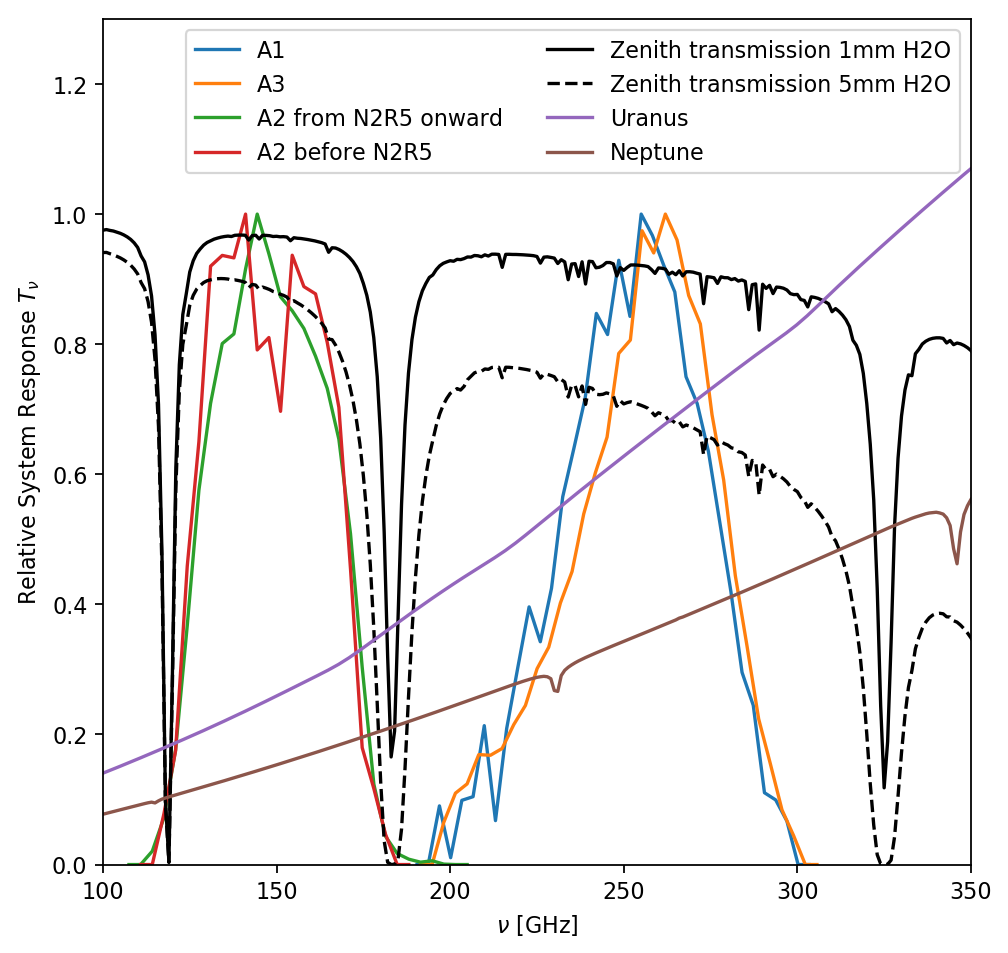
\includegraphics[width=0.75\textwidth]{Figures/SpectralBands/bandpasses_nika2.png}
\caption[NIKA2 transmission]{Relative system response of the three NIKA2 arrays as a
  function of frequency. For illustration we also plot atmospheric transmission obtained with the ATM model 
 \cite{ATM} for different values of precipitable water vapor. The spectra of ESA4 model of Uranus and ESA5 model of Neptune \cite{ESAmodel} in the frequency range are overplotted with arbitrary normalization.} 
 \label{spectralband1}
\end{center}
\end{figure}

 

The NIKA2 spectral bands were measured in the laboratory using a
Martin-Puplett interferometer built in-house \cite{durand}.  Both
arrays and filter bands were considered in the measurements. These
were obtained from the difference of two black bodies, hence they
include a $\nu^2$ Rayleigh-Jeans (RJ) spectral term.
Figure~\ref{spectralband1} shows the relative spectral response for
the three arrays (corrected of the RJ term).  Notice that array A2 was
replaced by a new one in N2R5 and that the spectral transmissions are
not the same (green and red lines in the figure).

The two arrays operating at 260 GHz, mapping different polarisations,
exhibit a slightly different spectral behaviour probably as can be
seen on figure \ref{spectralband1}. This may be explained by a tiny
difference in the silicon wafer and/or Aluminium film thicknesses. For
instance, the observed shift of the peak frequency, 265 GHz for the V
(A1) array versus 258 GHz for the H one (A3), can be explained by
about 5 microns change in the substrate thickness. Hereafter, the peak
frequencies are referred to as reference frequencies (150 and 260 GHz)
to which correspond the reference wavelengths (2.0 and 1.15 mm), see
tab.~\ref{tab:nika2summary}.


\begin{table}[th]
\begin{center}
\begin{tabular}{|l|l|r|r|r|r|r|r|}
\hline 
\multirow{3}{*}{Water vapor} & \multirow{3}{*}{Elevation} & \multicolumn{2}{|c|}{1 mm (H)} & \multicolumn{2}{|c|}{1 mm (V)} &
\multicolumn{2}{|c|}{2 mm} \\
 & & $\nu_eff$ & $\Delta \nu$  & $\nu_eff$ & $\Delta \nu$  & $\nu_eff$ & $\Delta \nu$ \\
 & & (GHz) & (GHz)  & (GHz)  & (GHz)   & (GHz)  & (GHz)  \\
\hline
\multicolumn{2}{|c|}{No atmosphere} & 254.71 & 49.21 & 257.39 & 48.05 & 150.93 & 40.72 \\
\hline
\multirow{4}{*}{1 mm $\rm H_2O$ $\rightarrow \tau_{225}=$0.067} & 90 deg &  254.46 & 48.72 & 257.12 & 47.95 & 150.93 & 39.71 \\
 & 60 deg & 254.42 & 48.68 & 257.08 & 47.93 & 150.92 & 39.60 \\
 & 40 deg & 254.33 & 48.57 & 256.98 & 47.89 & 150.88 & 39.32 \\
 & 20 deg & 254.00 & 48.21 & 256.62 & 47.77 & 150.75 & 38.45 \\
\hline
\multirow{4}{*}{2 mm $\rm H_2O$ $\rightarrow \tau_{225}=$0.120} & 90 deg &  254.26 & 48.74 & 256.91 & 48.06 & 150.64 & 39.34 \\
 & 60 deg & 254.20 & 48.70 & 256.84 & 48.07 & 150.60 & 39.19 \\
 & 40 deg & 254.02 & 48.60 & 256.65 & 48.08 & 150.48 & 38.80 \\
 & 20 deg & 253.43 & 48.30 & 256.01 & 47.93 & 150.13 & 37.62 \\
\hline
\multirow{4}{*}{3 mm $\rm H_2O$ $\rightarrow \tau_{225}=$0.173} & 90 deg &  254.06 & 48.76 & 256.70 & 48.19 & 150.39 & 39.03 \\
 & 60 deg & 253.97 & 48.73 & 256.60 & 48.21 & 150.32 & 38.84 \\
 & 40 deg & 253.71 & 48.65 & 256.33 & 48.28 & 150.14 & 38.35 \\
 & 20 deg & 252.86 & 48.41 & 255.40 & 47.86 & 149.60 & 36.94 \\
\hline
\multirow{4}{*}{5 mm $\rm H_2O$ $\rightarrow \tau_{225}=$0.278} & 90 deg &  253.67 & 48.82 & 256.28 & 48.45 & 149.96 & 38.47 \\
 & 60 deg & 253.51 & 48.81 & 256.11 & 48.44 & 149.84 & 38.22 \\
 & 40 deg & 253.10 & 48.77 & 255.68 & 48.26 & 149.54 & 37.58 \\
 & 20 deg & 251.74 & 48.67 & 254.20 & 47.75 & 148.68 & 35.82 \\
\hline
\multirow{4}{*}{8 mm $\rm H_2O$ $\rightarrow \tau_{225}=$0.437} & 90 deg &  253.08 & 48.94 & 255.66 & 48.42 & 149.38 & 37.76 \\
 & 60 deg & 252.84 & 48.93 & 255.39 & 48.35 & 149.20 & 37.42 \\
 & 40 deg & 252.21 & 48.94 & 254.71 & 48.16 & 148.77 & 36.64 \\
 & 20 deg & 250.12 & 49.38 & 252.43 & 47.91 & 147.52 & 34.57 \\
\hline
\multirow{4}{*}{10 mm $\rm H_2O$ $\rightarrow \tau_{225}=$0.542} & 90 deg &  252.70 & 49.00 & 255.24 & 48.38 & 149.04 & 37.34 \\
 & 60 deg & 252.39 & 49.01 & 254.92 & 48.29 & 148.82 & 36.97 \\
 & 40 deg & 251.62 & 49.11 & 254.08 & 48.13 & 148.31 & 36.12 \\
 & 20 deg & 249.07 & 49.75 & 251.28 & 48.24 & 146.85 & 33.93 \\
\hline
\end{tabular}
\caption[Effective frequencies and bandwidthes]{Effective frequencies (for Uranus) and bandwidth of the NIKA2 bands for
  various atmospheric conditions and elevation.}
\label{tab:bandwidths}
\end{center}
\end{table}

%What actually matters more than the ``central frequency'' that depends on many
%assumptions and definitions are the bandpasses. We should make available in a
%.fits file, clearly, our bandpasses to avoid future misunderstanding and propagation of
%false numbers. Official values should be 150 and 260~GHz. We should also clearly
%state that these measured bandpasses were done with the difference of two
%black-bodies, hence they include a $\nu^2$ RJ term.\\

{\color{red} LP: to be moved to Section Calibration ? Opacity ? }


The total system response is the multiplication of the atmospheric
transmission with the relative system response. To derive the
atmospheric transmission, we use GILDAS ATM 2009 model \cite{ATM}, computed for
the IRAM 30-m telescope, with so called {\it midlatwinter} conditions. We select in the model
grid an atmosphere with $T=268.3 \ {\rm K}$ and a pressure of $703.5 \ {\rm hPa}$. The
effective frequency of the passband is defined by:
\begin{equation}
\nu_{eff}( \sec \delta, mm_{H_{2}O}) = \frac{ \int_{0}^{+\infty} S_{\nu}
  T_{\nu}(\sec \delta, mm_{H_{2}O}) \nu d\nu } { \int_{0}^{+\infty} S_{\nu} T_{\nu} d\nu}
\label{eq:nueff0}
\end{equation}

{\color{blue} FXD: we should integrate over SOmega (nu-2). For
  MartinPuplett measurements, the source spectrum was RJ (nu2) so that
  cancels out to find Tnu. Snu is for an extended source. Deltanu
  should be with respect to a spectrum, for example RJ. I think the
  table 2.1 is not very useful. It could be a figure (nueff as a
  function of tauLOS (elevation is not relevant)? or just few numbers:
  we should at the end state what is nueff and deltanu for average
  conditions. Nomenclature: 1mm(H) is not the usual denomination... }


where $T_{\nu}$ is the total system response, normalized between
0. and 1. (i.e. a relative response as a function of the frequency),
hereafter referred to as RSR (Relative System Response), $S_{\nu}$ is
the source spectrum. Table~\ref{tab:bandwidths} lists this effective frequency,
computed for Uranus spectrum (ESA4 model, \cite{ESAmodel}), for different atmospheric
water vapor contents and different elevations. 
Table~\ref{tab:bandwidths} also list the bandwidth, defined as:
\begin{equation}
\Delta\nu = \int_{0}^{+\infty} \frac{T_{\nu}}{Max(T_{\nu})}
d\nu
\end{equation}
where the $Max(T_{\nu})$ ensure the RSR span the whole 0.0 to 1.0 range.

From Table~\ref{tab:bandwidths}, we see that the 2 mm band is somewhat
sensitive to the atmospheric conditions, especially at low
elevation. Note that these effective frequencies are {\em not} the
reference frequencies for the band, respectively 150 GHz and 260 GHz
for the A2 and A1, A3 arrays. These reference frequencies are chosen
as round numbers in the middle of the bands to define NIKA2
photometric system as will be discussed in section~\ref{se:cal_HA}.

%
% LP: the paragraph below rather belongs to the Opacity section
%
%Using the NIKA2 bandpasses for N2R9, we can integrate the ATM
%atmospheric model to compute the expected ratio between the
%atmospheric opacity of the two NIKA2 channels. 
%Figure~\ref{thopacities} shows the atmospheric opacity
%ratio of the 2 and 1 mm channels as a function of the opacity for the
%1 mm one.

%\begin{figure}[ht] % Inline image example
%\begin{center}
%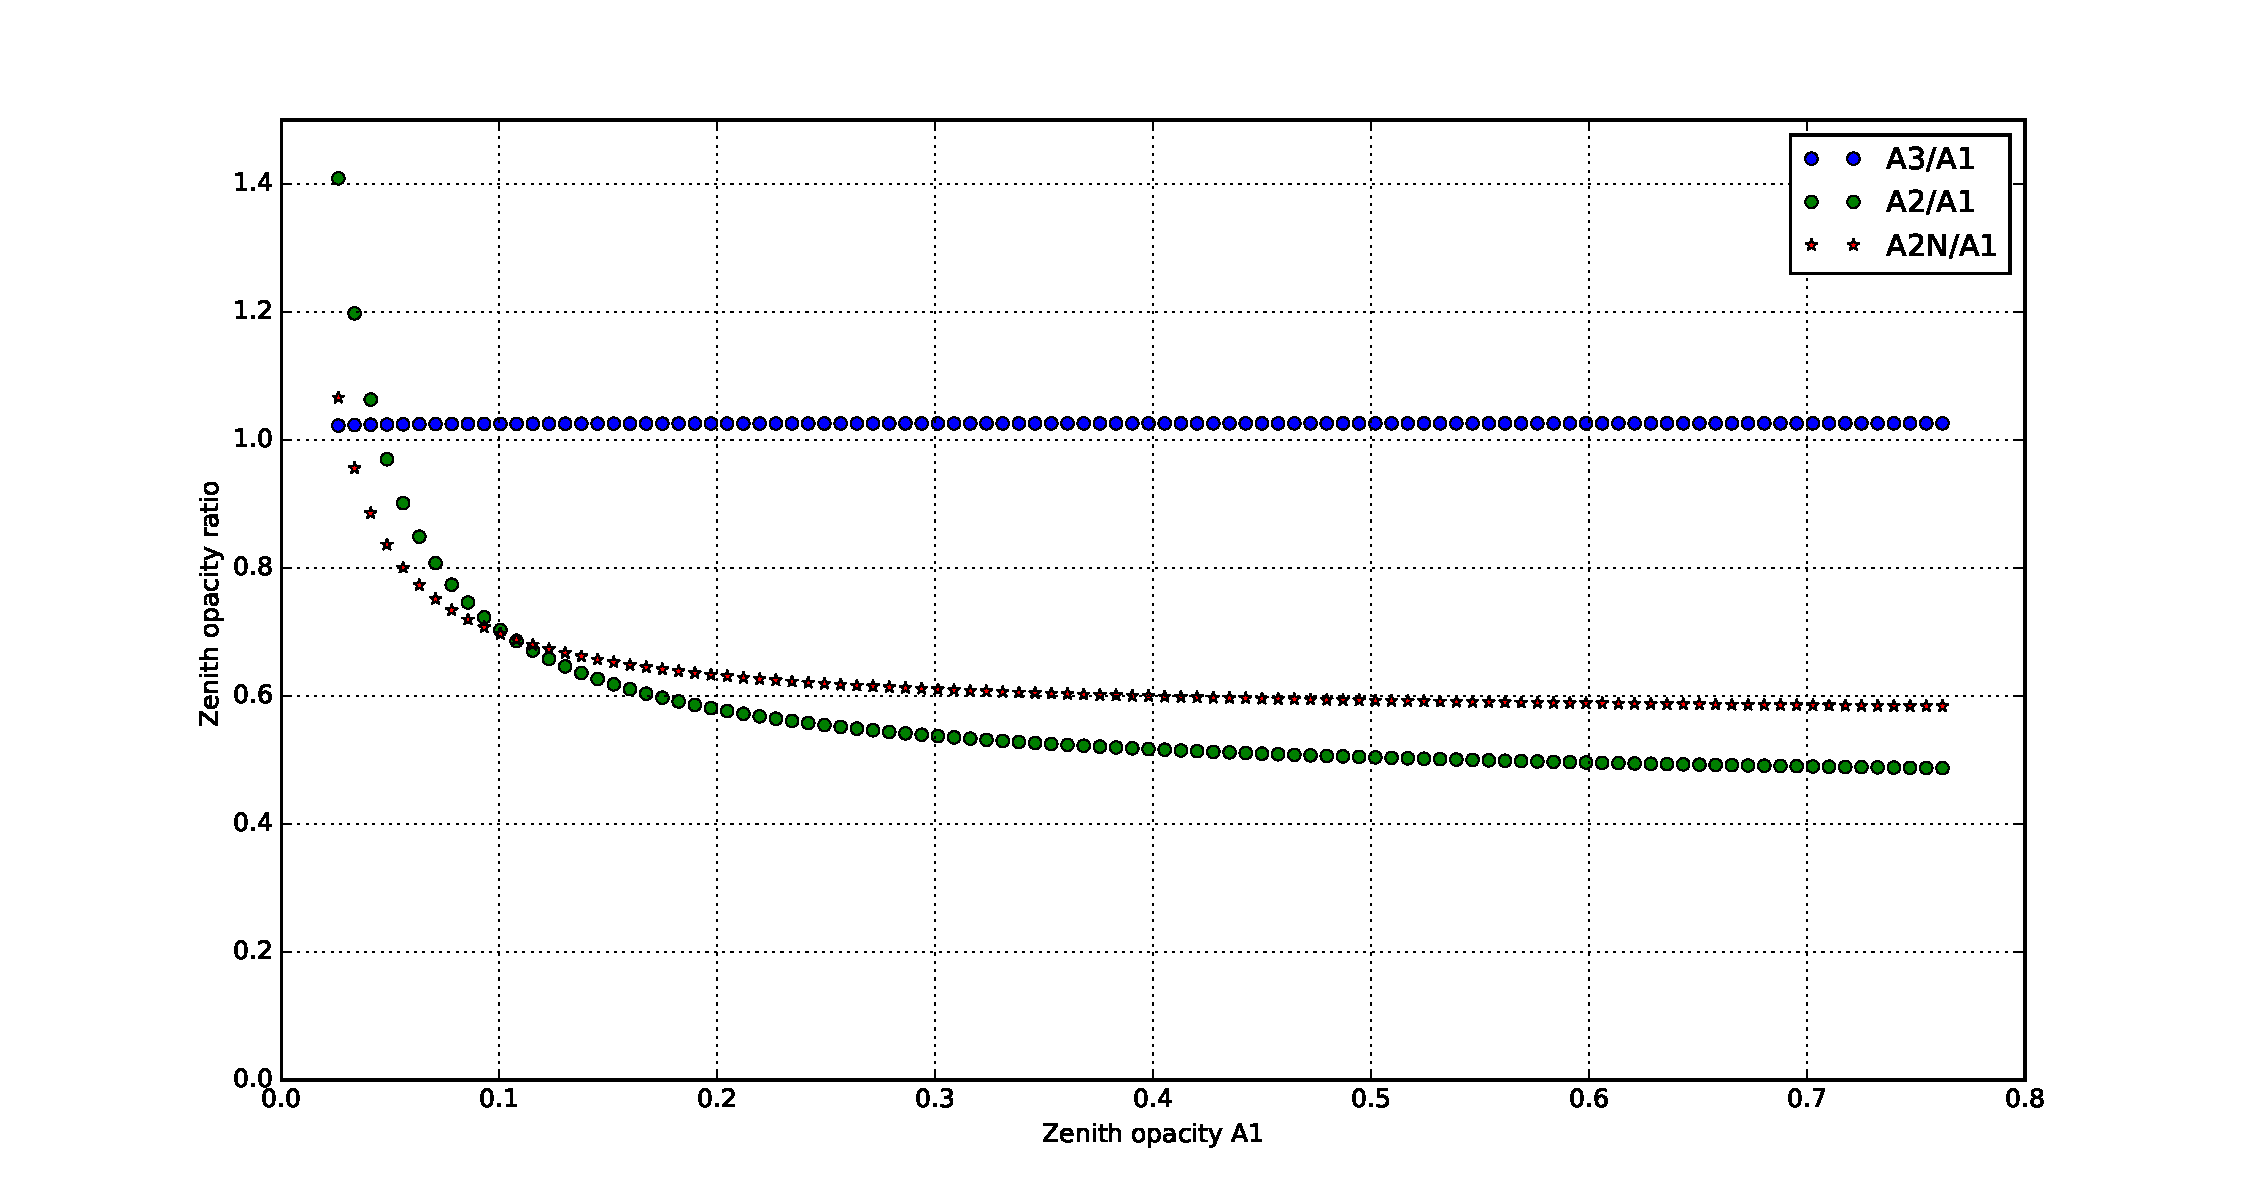
\includegraphics[width=\textwidth]{Figures/SpectralBands/opacity_ratio_vs_tau1.pdf}
%\caption{Expected atmospheric opacity ratio of the 2 and 1 mm channels as function 
%of the opacity at 1 mm. {\bf FM: what is A2N/A1 ?} {\bf FM: why is A3/A1=1 ?}}
%\label{thopacities}
%\end{center}
%\end{figure}





%-------------------------

\subsection{Cryogenics}

The optimal operation of the detectors is achieved at a temperature of around
150\,mK, well below the Aluminium superconducting transition. For this reason,
NIKA2 employs a custom dilution fridge to cool down the focal plane, and the
refractive portion of the optics, for a total mass around 100 kg, deeply in the
sub-Kelvin regime. Despite the complexity and size of the system, the operation
of NIKA2 does not require external cryogenic liquids and is fully remotely
controllable.

\subsection{KIDs and electronics}
\label{se:array}

The 150\,GHz channel is equipped with A2 that is an array of
616\,pixels, arranged to cover a 78\,mm diameter circle. Each pixel has a size of
$2.8\times2.8\textrm{\,mm}^2$. The array A2 is connected over four different
readout lines. In the case of the 260\,GHz band detectors, the pixel size is
$2\times 2\mathrm{\,mm}^2$, to ensure a comparable sampling of the focal
plane. In order to fill the two 260\,GHz arrays A1 and A3, a total of 1,140 pixels are
needed in each of them. The focal planes are all based on thin Aluminium films
deposited by e-beam evaporation under ultra-high vacuum conditions over a
Silicon substrate.

The key advantage of the KID technology is the simplicity of the cold
electronics and the multiplexing scheme. In NIKA2, each block of around 150
detectors is connected to single coaxial line providing the excitation and the
readout at the two ends. Each of the readout lines is linked to the input of a
cryogenic (4 K) low-noise amplifier. The warm electronics required to digitize
and process the pixels signals is composed of twenty custom readout cards (one
per feed-line).

%In this document, the 2\,mm array is called A2, while the two 1\,mm arrays are
%called A1 and A3.


\subsection{KID photometry and tuning}

\begin{figure}[!b]
\begin{center}
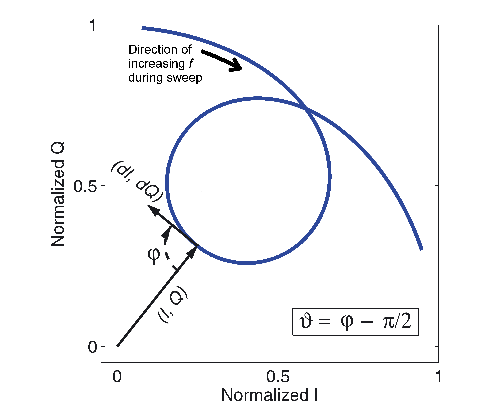
\includegraphics[width = 0.7\textwidth]{Figures/resoCircle-eps-converted-to.pdf}
\caption[KID resonance circle]{Sample resonance circle in the IQ plane. Both the
  tuning procedures are based on the measurement of the angle $\vartheta$
  between the two vectors ($I, Q$) and ($dI, dQ$)}
\label{figResoCircle}
\end{center}
\end{figure}

Kinetic Inductance Detectors are superconducting resonators whose resonance
frequency shifts linearly depending on the incoming optical power. The measure of such
frequency shift $\Delta f$ is what allows us to use KID as mm-wave detectors.

For the KID readout, an excitation signal is sent into the cryostat on the
feedline coupled to the KID. The transmitted signal can be described by its
amplitude and phase, or, as is common practice for KID, by its components that
are In-phase ($I$) and in Quadrature $Q$ with respect to the excitation
signal. When a frequency sweep is carried around a KID resonance, the
transmitted signal makes a sort of circle in the $I-Q$ plane, as shown
in Fig.~\ref{figResoCircle}.
The goal is now to relate the variations $(\Delta I, \Delta
Q)$ along this circle induced by incident light to the $\Delta f$. For this, the
electronics modulates the excitation frequency at about 1\,kHz with a known
$\delta f$ frequency variation and the read out gives the induced $(dI,
dQ)$. Projecting linearly $(\Delta I, \Delta Q)$ on $(dI, dQ)$ therefore
provides $\Delta f$. This value, in Hz, is the raw input timeline to the
pipeline and will be futher calibrated into astronomical units
(sect.~\ref{se:calibration}). For historical reasons, this way of deriving KID
signals has been nicknamed \emph{RfdIdQ}. More details on this process are given
in \cite{Calvo13}.\\

Not only incident astronomical light reaches the KIDs and contributes to Cooper
pair breaking. Any change in the background optical load (due, for example, to changes in
the atmospheric transmission or in the elevation) contributes as well to the
shift of the resonances. In order to maximize the sensitivity of a KID, the
excitation signal used to read it out must always be near its resonance
frequency. We therefore have developped a tuning algorithm that takes care of
this optimization. Tunings are performed during the first subscan of each
observation in order to be optimally tuned at the same elevation and sky
conditions as the source. It takes only a few seconds when the $f_{tones}$ are
close to the current functionning point. In order to always be in these
conditions, continuous tunings are done between two scans when NIKA2 is not observing.

A specific case is when we do {\tt skydips}. In this case, we tune all the KIDS
at the beginning of each subscan/elevation step on purpose to monitor the
induced variation of $f_{tone}$ by the sky load.



\clearpage
%----------------------------------------------------------------------------------------
%	OBSERVATION MODES
%----------------------------------------------------------------------------------------
\section{Observations at the 30 meter telescope}
\label{se:observation}

\section{Calibration and commissioning observations at the 30\,m telescope}% {\color{YellowGreen} Nico}}

This section presents the different observation modes that have been used with
\nika\ for both commissioning and scientific purposes. Some of them are common
to usual IRAM observing modes (e.g.~''on the fly'' raster scans), some of them
have been designed specifically for \nika\ (e.g.~the focus sequence). We start
by a short overview of a typical set up sequence at the beginning of
an observational run. This
will put each observation mode in perspective. Then we go into more details
about the performances of the system.

\subsection{Overview of different types of scans}

Once the KIDs are tuned and \nika\ is ready for observations, before actually
observing a scientific target, one needs to adjust the focus and pointing of the
telescope. In the case of EMIR typically, these two parameters are adjusted iteratively by
alterning ``pointing'' (\aka\ ``cross'') and ``focus'' scans to optimize the
centering of a bright point source on a reference detector and to maximize the
incoming flux on it. With \nika\ , mostly due to absence of horns, this
procedure is not optimal. Indeed, it was noticed that the position of the source
moved by several arcsec with the displacement of M2
\vu{during the focus procedure} and this would alter the flux
measurement on a fixed reference position too much to enable focus
optimization.

To solve this issue we have designed a specific focus procedure that takes
advantage of the dense sampling of the FOV that allows to map a source with only
a few subscans. We perform a series of five successive short raster scans of a
bright point source at five M2 position offsets along the optical axis.%, typically
%$\{-0.8, -0.4, 0, 0.4, 0.8\}$\,mm w.r.t.~the current $z$-focus (which
%is usually the previous optimal $z$-focus value).
We then analyse each map to optimize the $z$ position of M2. More details are given in
Sect.~\ref{se:axial_focus}.
Once the focus is correctly determined, the pointing
corrections are derived from an EMIR like pointing calibration scan
(Sect.~\ref{se:pointing}). The instrument is then ready to observe scientific
targets.

\subsection{Axial focus}
\label{se:axial_focus}

\begin{figure}[ht!]
\begin{center}
  %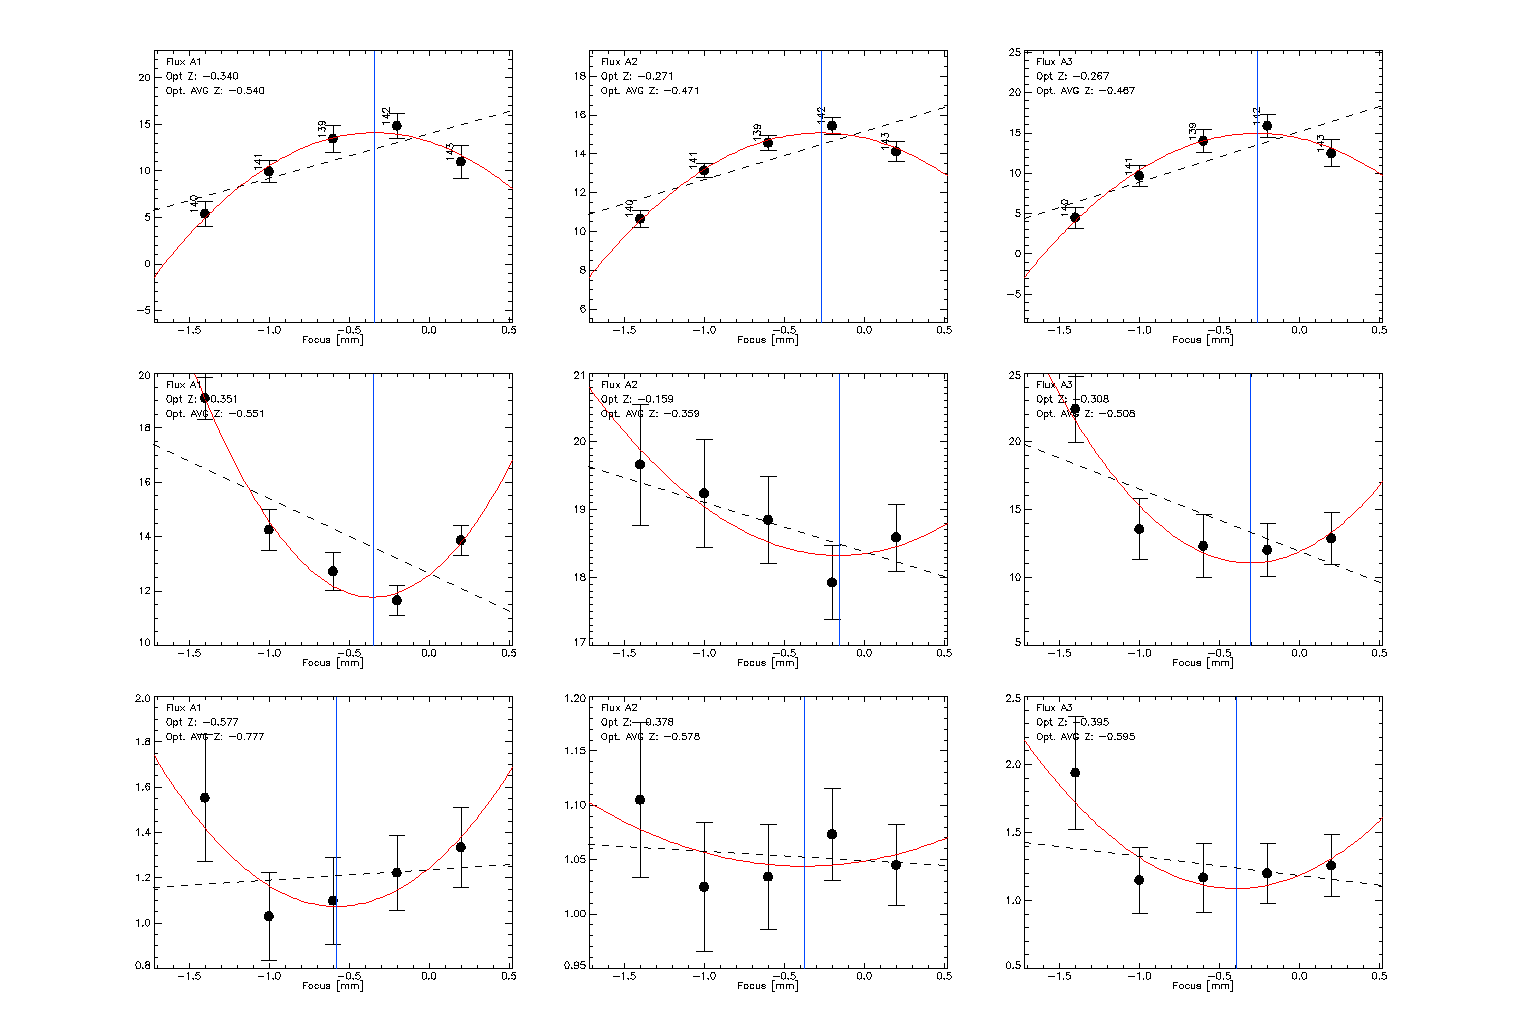
\includegraphics[clip, angle=0, trim={1.5cm, 1cm, 1.5cm, 1cm},
  %width=\textwidth]{Figures/plot_20170419s143.png}
  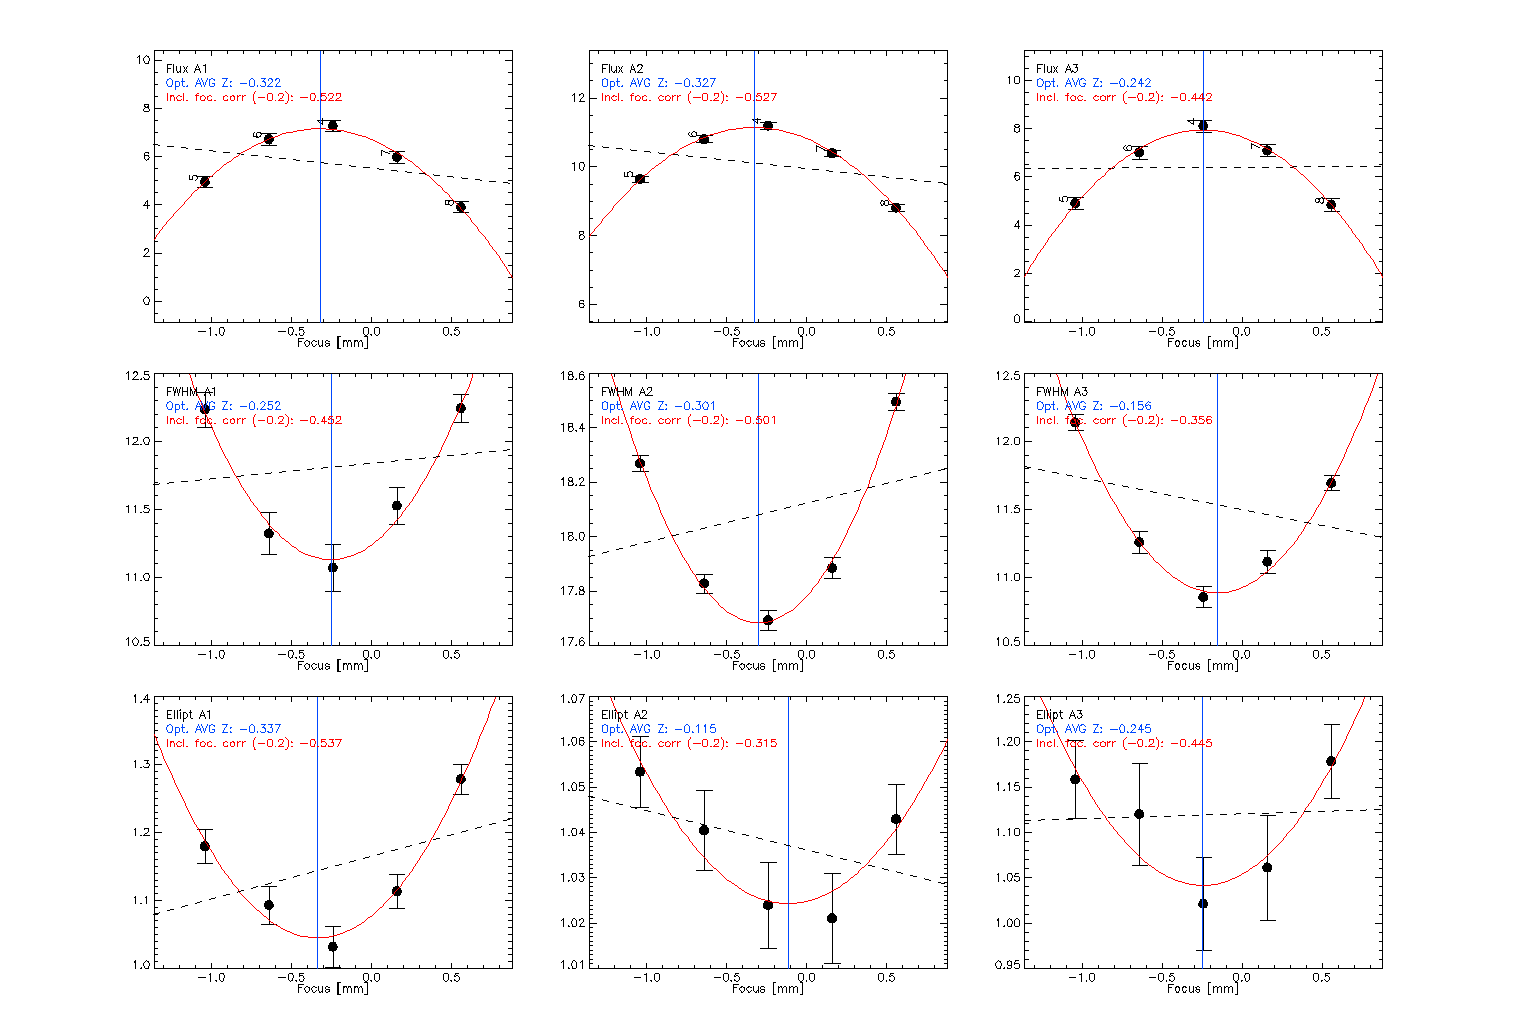
\includegraphics[clip, angle=0, trim={3cm, 0.5cm, 3cm, 1.5cm}, width=\textwidth]{Figures/plot_20180120s8_zfocus.png}
\caption[Axial focus measurement]{Example of axial focus measurement using a
  \emph{focus$\_$OTF} observation of the bright quasar 3C84 (\aka\ 0316+413) during N2R14 in good observing conditions (scans ID: from '20180120s4' to '20180120s8'). \vu{Flux (first
  row), FWHM (second row) and ellipticity (third row) measurements are
  shown as a function of the axial focus offsets for Array 1 (first
  column), Array 2 (second column) and Array 3 (third column). The
  best-fitting parabola is shown in red. To help the observer
  assessing the parabolic fit quality, the best-fit linear model is also drawn
  with dashed black lines.} 
  The blue vertical line locates the best-fitting $z$-focus value of
  each fit. The optimal focus values derived from flux
  maximization and FWHM minimization agree to better than 0.1\,mm in these
  conditions of observation. While ellipticity may be often regarded as a confirmation
  more than a decisive criterion (due to larger uncertainty on its measure), the
  associated minimum is also in good agreement with the values derived from flux
  and FWHM measurements in this example taken in stable atmospheric conditions.}
\label{fig:focus-example}
\end{center}
\end{figure}

The best axial focus in the central region of the arrays is estimated using the
so-called \emph{focus$\_$OTF} PAKO script, which produces a series of five $1'
\times 5'$ OTF scans at various values of the focus in $0.4~\rm{mm}$ steps
around an \emph{a priori} value $z_0$, namely
$z \in \{-0.8, -0.4, 0, 0.4, 0.8\} + z_0$.
Elliptical Gaussian fits on the reconstructed maps provide estimates of
the flux and FWHM along minor - and major - axes for each focus. Parabolic fits are
then used to determine the best focus. We consider three estimates: i) $\hat
z_{\rm{peak}}$ the focus that maximizes the estimated flux, which is the
amplitude of the 2D Gaussian, ii) $\hat z_{\rm{fwhm}}$ the focus that minimizes
the geometrical FWHM, defined as the quadratic mean of $\rm{FWHM}_{\rm{major}}$
and $\rm{FWHM}_{\rm{minor}}$, and iii) $\hat z_{\rm{ellipt}}$ the focus that
minimizes the beam ellipticity, defined as
$\rm{FWHM}_{\rm{major}}/\rm{FWHM}_{\rm{minor}}$. Fig.~\ref{fig:focus-example}
shows an example of such a sequence. When deciding on the focus to apply, we
give priority to the optimal flux, taking an average between values on A1 and
A3: there is little difference between the two and the 2\,mm channel is
less sensitive to the focus change than the 1\,mm.

As presented in more details in Sect.~\ref{sec:focus_surfaces}, the focus
surface is not strictly flat across the FOV. The way sources are scanned in
this \emph{focus\_OTF} sequence is designed to save time but it gives more weight
to the central KIDs. Hence, the optimal focus derived from the fits is
biased. To account for the curvature of the focus surfaces and optimize the
average focus across the FOV, we add -0.2\,mm to the best-fit focus value as derived
in the previous paragraph. \vu{This focus offset is derived using ZEMAX
simulation and it is verified on data as discussed in
Sect.~\ref{sec:focus_surfaces}.}

\subsection{Lateral focus}
\label{sec:focus_X_Y}

Like in the $z$ (optical axis) direction, it is possible to control the position
of M2 along the $x$ and $y$ directions. We have tried to determine if there was
an optimal position in the $(x,y)$ plane that would improve further measurements
with \nika. We have applied the same procedure as the one described in
Sect~\ref{se:axial_focus}, this time varying the position of M2 along $x$ or $y$
rather than along $z$. Examples of such observations are presented on
Figs.~\ref{fig:X_focus} and \ref{fig:Y_focus}. While the forced parabola fit
guides the eye towards optimization, one should note the size of the error bars
and the relatively low variations compared to M2 displacements along the $z$
axis. This is expected from optical simulations and experience on
EMIR. Figs.~\ref{fig:X_focus} and \ref{fig:Y_focus} also show as complement,
images of the residuals of the intensity maps at each M2 position after the
subtraction of an elliptical gaussian fitted only on a disk of 6 and 15\,arcsec
(1 and 2\,mm resp.) around the maximum location and outside a ring of 100\,arcsec
away from the maximum (to fix the background while not being affected by the
side lobes). These maps of residuals are meant to help to decide on a minimization
criterion and $x$ or $y$-focus value.

While we have performed ``many'' of such observations and explored the entire
parameter space of the $(x,y,z)$~triplet position in a reasonable range of
several millimeters around a fixed position, it has not been possible to
demonstrate that any $(x,y)$ positions would improve significantly the
focusing of the whole system compared to the nominal $(0,0)$ reference
position. \vu{This confirms the experience of the IRAM staff with EMIR and
HERA who only act on this $(x,y)$ position about once a year after
specific, dedicated and delicate measures. This effort is necessary
to find an optimum lateral focus position which is stable with
elevation. For \nika\, the adopted strategy has been not to change the
lateral focus parameters and only rely on $z$-focus optimization for
observations. However, lateral focus measurements with NIKA2 have to be
scheduled in the future.} 
%We have therefore concluded that we should not change these
%parameters for \nika\ and only rely on $z$-focus optimization for observations.

\begin{figure*}[h!]
\centering
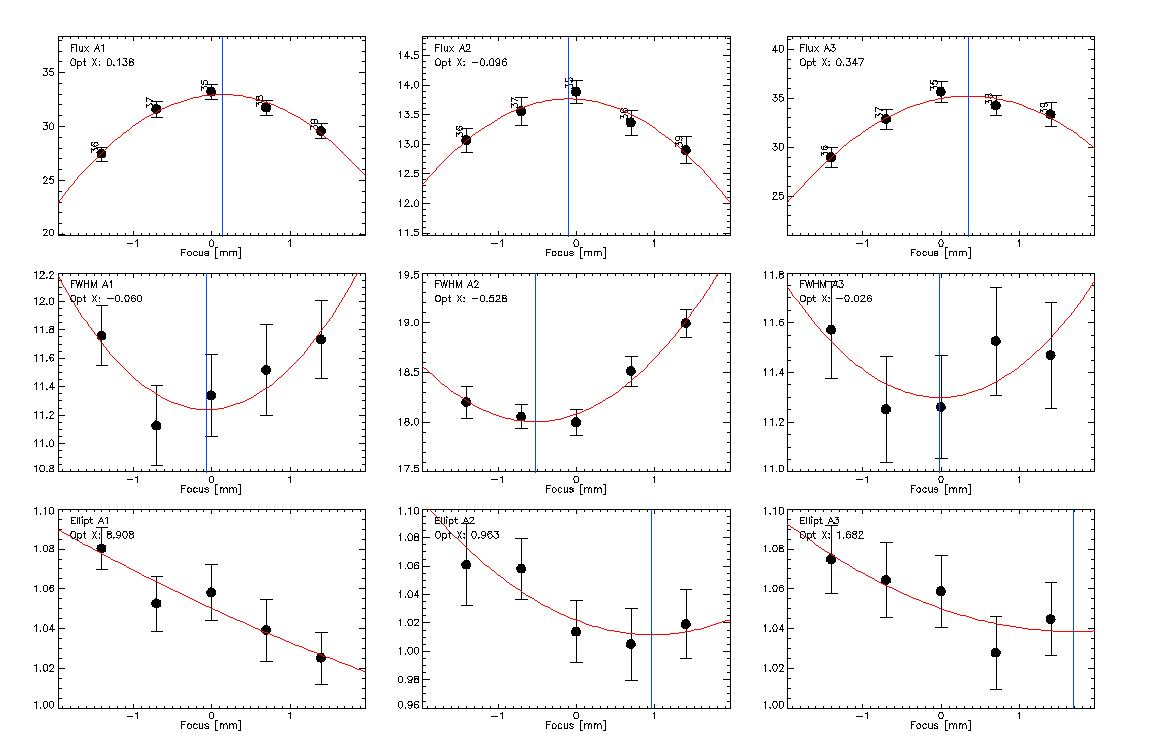
\includegraphics[height=8cm]{Figures/plot_20170223s39.png}
\hspace{0.5cm}
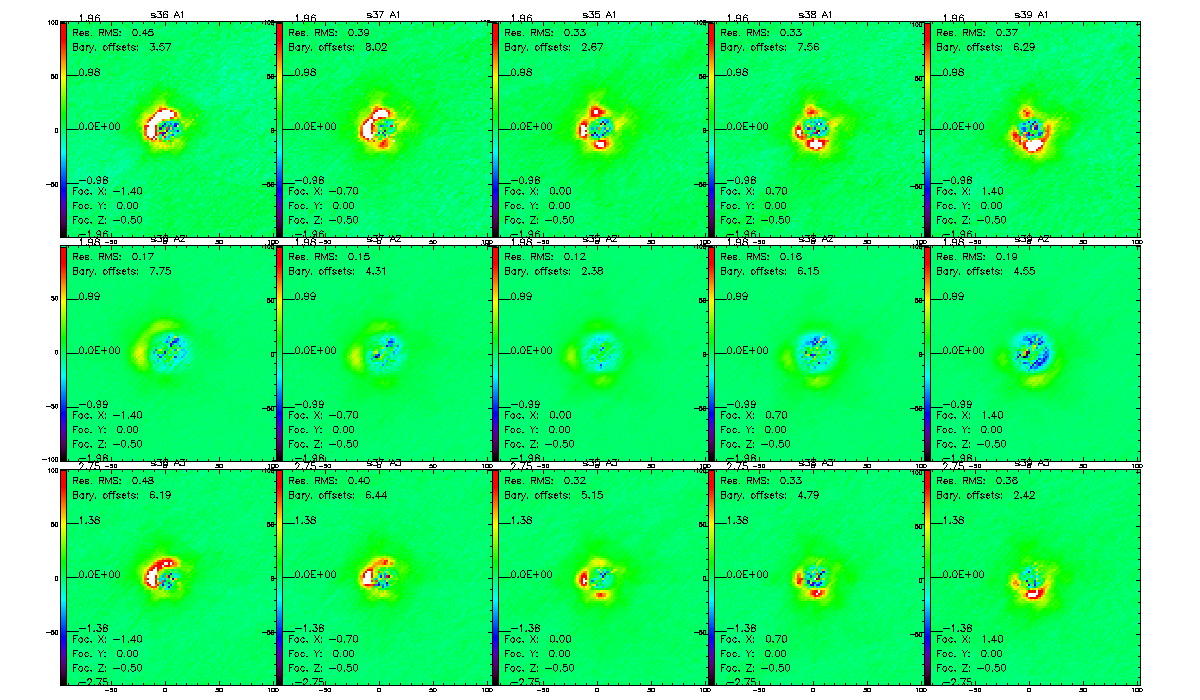
\includegraphics[height=8cm]{Figures/residuals_focus_otf_20170223s39.png}
\caption[Lateral X focus measurements]{\emph{top panel: }X-focus measurement using a
    parabolic fit of the flux, beam FWHM and ellipticity on a sequence
    of five OTF scans on Uranus (20170223s39-43) \emph{bottom panel: }Beam residuals
    after subtracting a model of the main beam for each OTF-scan of the X-focus
    session. (N2R9)}
\label{fig:X_focus}
\end{figure*}

\begin{figure*}[h!]
\centering
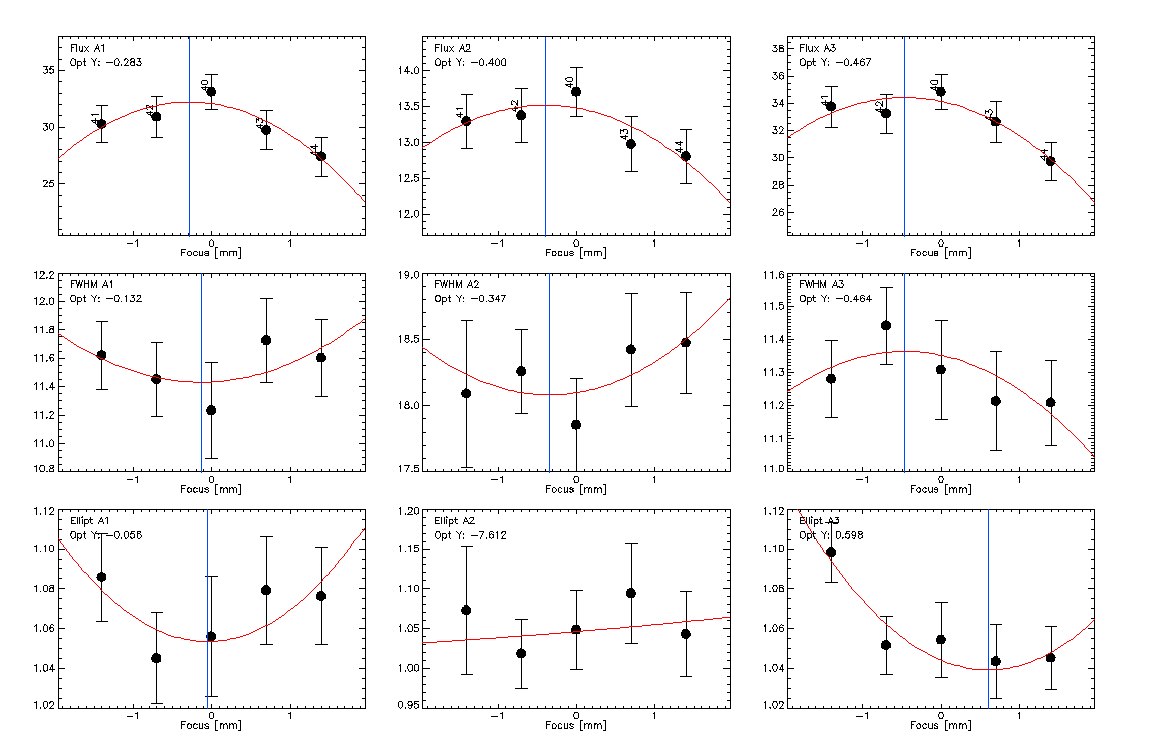
\includegraphics[height=8cm]{Figures/plot_20170223s44.png}
\hspace{0.5cm}
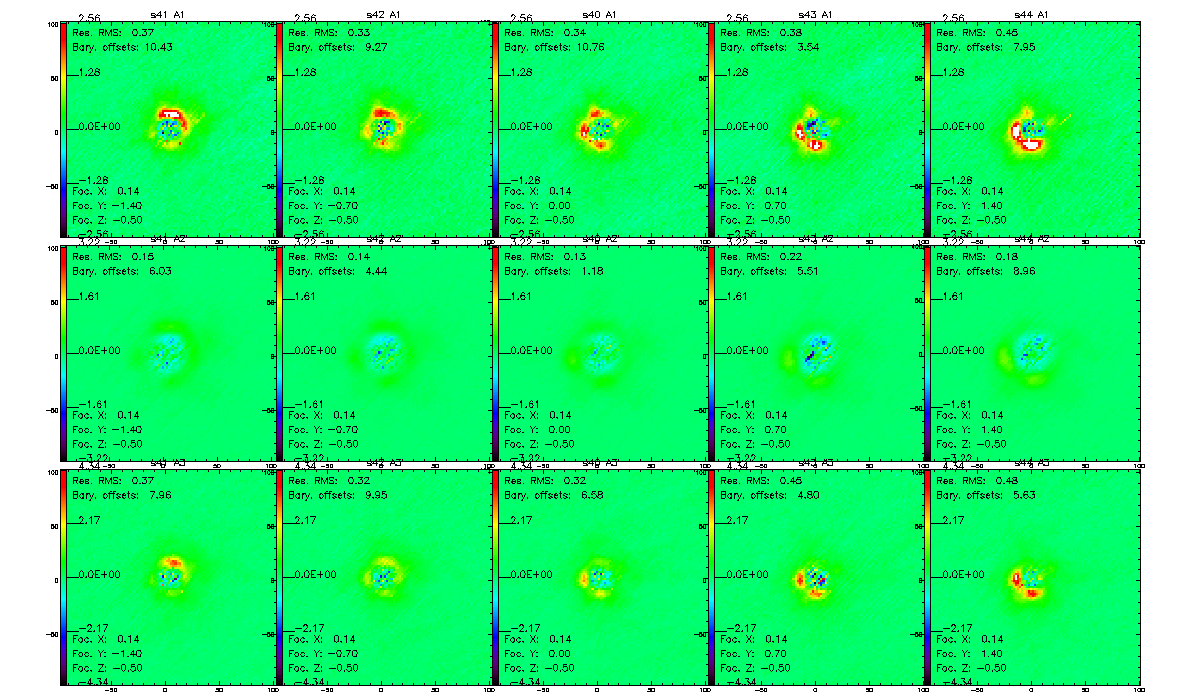
\includegraphics[height=8cm]{Figures/residuals_focus_otf_20170223s44.png}
\caption[Lateral Y focus measures]{\emph{top panel: }Y-focus measurement using a
    parabolic fit of the flux, beam FWHM and ellipticity on a sequence
    of OTF scans on Uranus (20170223s44-48). \emph{bottom panel: }Beam residuals
    after subtracting a model of the main beam for each OTF-scan of the Y-focus
    session. (N2R9)}
\label{fig:Y_focus}
\end{figure*}


\subsection{Pointing}
\label{se:pointing}
% + RTA pointing estimate method
% + pointing model
% + pointing error (scan-to-scan scattering)

Once the instrument is correctly focused, we can estimate pointing corrections
before scientific observations.
%The procedure that is used is very similar to
%that used for EMIR and is described in the next subsection.
\vu{Even though EMIR only has a single pixel on the sky, the pointing procedure
used for NIKA2 is very similar and is described in the next subsections.}
%It was used
%repeatedly during pointing sessions to derive the pointing model of.

\paragraph{Pointing monitoring}

\begin{figure}[ht!]
\begin{center}
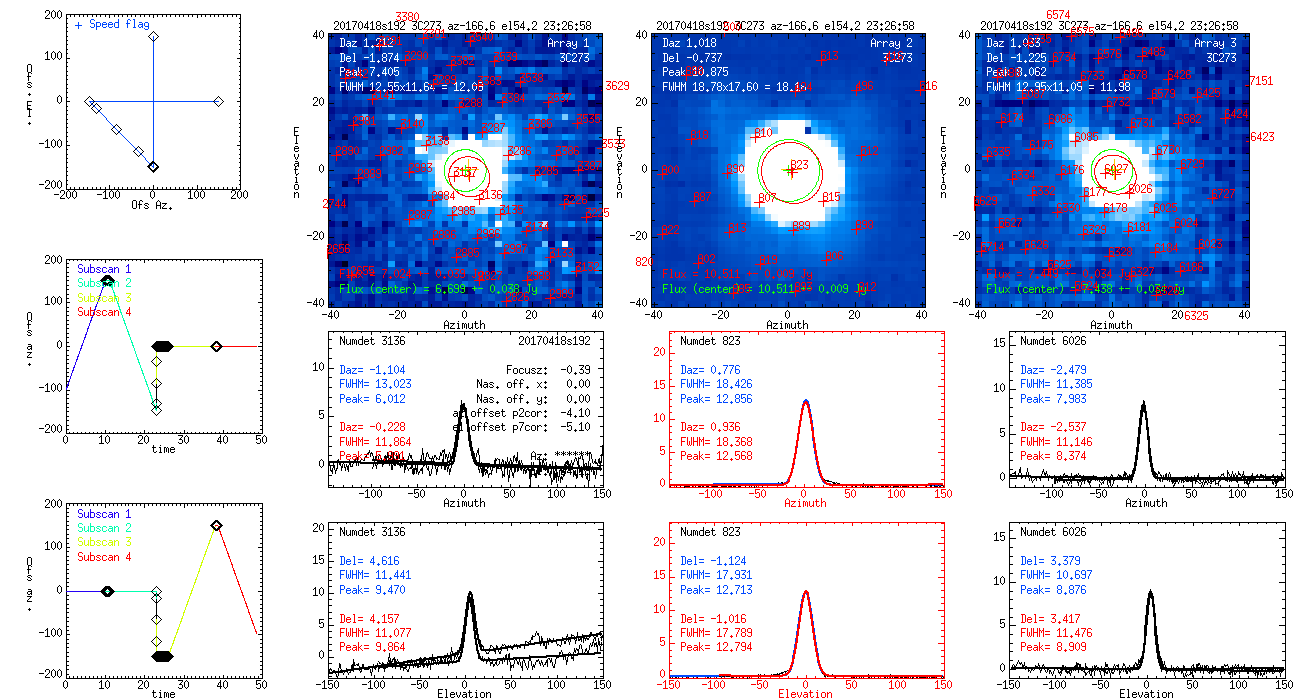
\includegraphics[clip, angle=0, scale = 0.30]{Figures/plot_20170418s192.png}
\caption[Summary plots of the reduction of pointing scan.]{Top plots
  show the combined map for array 1, 2 and 3, which enable a check of
  the overall quality of the scan, while bottom plots show the set of azimuth
  and elevation profiles for one reference detector per array. The
  reference detector per array is highlighed with a red cross in the
  centre of the map. The pointing reference detector of
  \nika\ is the 2\,mm reference detector, the azimuth
  and elevation profiles of which are shown in the central bottom
  plot. The location of the peak in azimuth and elevation, as observed by the
  reference detector gives the pointing offsets of the current scan.
}
\label{fig:ptg}
\end{center}
\end{figure}

\begin{figure}[ht!]
\begin{center}
\includegraphics[clip, angle=0, trim={0, 0, 3cm, 0}, width=0.65\textwidth]{Figures/pointing_stats_N2R9.eps}
\caption[Pointing session results]{Pointing offsets during Run9 observations,
  before (blue to green) and after (yellow to red) the
  derivation of Nasmyth offsets with a pointing session on Feb.~26th, 2017.}
\label{fig:pointing_stats_n2r9}
\end{center}
\end{figure}

Based on general operating experience at the 30\,m telescope, we use the so-called
{\em pointing} or {\em cross} scans to monitor the pointing during observations. The
telescope executes a back and forth scan in azimuth and a back and forth scan in
elevation, centered on the observed source. Looking at the timeline profiles of
the reference detector, we fit gaussian profiles and derive the current pointing
offsets of the system in azimuth and elevation. These offsets can then be passed
to PAKO to recenter the next scan (Fig.~\ref{fig:ptg}).

\paragraph{Pointing session}
\label{se:pointing_session}

Such scans and their analyses are also used to improve the pointing model of
\nika. A pointing session consists in observing about 30 sources on a wide range
of elevations \new{and azimuth angles} while monitoring the pointing offsets
that are measured for each observation. These offsets are then passed to the
IRAM staff who finds the pointing model parameters that minimize and symmetrize
the scattering of these offsets. Based on these results, the Nasmyth offsets
parameters that enter the IRAM pointing model are
adjusted. Fig.~\ref{fig:pointing_stats_n2r9} shows the pointing corrections that
had to be applied during Run9, before and after the modification of the Nasmyth
offsets. The dispersion of the offsets is the figure of merit of the pointing
corrections. Their distribution after the corrections (in yellow to red) is
clearly more symmetric and narrower than before. During N2R9 run, \vu{the rms of
  the residual scatter after the
  correction} was 1.62\,arcsec rms in azimuth and 1.37\,arcsec rms in elevation.

\subsection{Skydip}
\label{se:skydip}

A {\tt skydip} scan \new{with NIKA2} consists in a step-by-step span
of a large range of elevations. This is used in order to calibrate the
KIDs response to the atmosphere for opacity derivation, as discussed in
Sect.~\ref{se:opacities}.
\new{Whereas with the heterodyne receivers, skydips can be
  conducted continuously slewing the telescope in elevation, this
  option is not feasible with NIKA2, as the KIDs need to be retuned
  for a given airmass.}
For that purpose, a NIKA2 skydip comprizes eleven steps in
the elevation range from 19 to 65 degrees, regularly spaced in
airmass. For each step, we acquire about twenty seconds of time traces
to ensure a precise monitoring of each KIDs. KIDs are tuned at the beginning of
each subscan (hence once per airmass). The variation of their resonance
frequency reads

\begin{equation}
  %\ftone^k  = C_0^k - C_1^k T_{atm}[1-e^{-\tau/\sin\delta}]
  f_{\rm{reso}}^k  = C_0^k - C_1^k T_{atm}[1-e^{-\tau/\sin\delta}]
\label{eq:skydip_1}
\end{equation}

An illustration is presented on Fig.~\ref{fig:ftone_vs_elev}. More details on
the analysis of these {\tt skydip} scans are given in Sect.~\ref{se:opacities}.

\begin{figure}[ht!]
\begin{center}
  \includegraphics[clip, angle=0, scale=0.75]{Figures/skydip_report.eps}
\caption[skydip]{Variation of the resonance frequency of a KID
  \new{$f_{\rm{reso}} = \ftone + \delta \ftone$},  as a function of the
  elevation during a {\tt skydip} scan.}
\label{fig:ftone_vs_elev}
\end{center}
\end{figure}

\subsection{\bms}
\label{se:beammaps}

A \bm\ is \vu{a scan procedure to map} a bright and compact
source, most of the time a planet, with
an elevation step small enough to meet Nyquist sampling of the 1\,mm beam,
namely 4.8~arcsec. We observe the planet with a raster scan in (az,el)
coordinates of $13\times7.8$~arcmin$^2$, either with fixed elevation subscans or
fixed azimuth subscans. The former has the advantage of low air mass variation
across a subscan, the latter offers an orthogonal scan direction to the former:
the combination of both gives a more accurate determination of the far side
lobes. The scan size ensures that the entire FOV is observed with good margins
for beam mapping even on the edges and good margins for baseline derivation and
subtraction in the scanning direction. During subscans, the telescope travels at
65\,arcsec/s. This value results of a tradeoff between the need to scan as
fast as possible to minimize atmospheric contamination and the
necessity to keep subscans no shorter than 10\,s (telescope
constraint). The need to have Nyquist sampling of
the beams along the scan direction translates into a maximum speed of 110\,arcsec/s
for our nominal acquisition rate of 23.8\,Hz and is thus largely met. Subscans
last 12\,s, the entire scan lasts about 25\,min, which is short enough to prevent
%too much variation of KID tuning under stable weather conditions on
%this timescale.
\sam{losing the signal due to atmosphere-induced (1/f) background variations that would
  move the resonance away from the tone probing it.}


More details on these observations are given in Sect.~\ref{se:fp_reconstruction}
where we describe how to actually exploit them to derive individual KID
properties.


\clearpage
%----------------------------------------------------------------------------------------
%	CALIBRATION PIPELINE
%----------------------------------------------------------------------------------------
\section{Calibration and Data reduction overviews}
\label{se:calib_pipeline}

%hi

\subsection{Overview of the calibration pipeline}

The steps to go from raw timeline data in Hertz to calibrated data in Jansky per beam comprize:
\begin{itemize}
\item[] Opacity correction
\item[] Field-of-view geometry and KIDs selection
\item[] KID-to-KID intercalibration (flat fielding)
\item[] Absolute calibration  
\end{itemize}


\subsection{Data reduction summary {\color{blue} Nico}}

The performance assessment relies on a data reduction pipeline that consists of the following steps:
\begin{itemize}
\item[] reading of the raw timeline 
\item[] implementation of the calibration
\item[] substraction of the correlated part of the noise 
\item[] projection of the timeline onto maps
\end{itemize}


\subsection{Data selection {\color{blue} Laurence}}
\label{se:data_selection}

For calibration and performance assessment, we select scans in average
observing conditions by performing mild selection cuts. These scan
cuts rely on zenith opacity estimates in NIKA2 bands $\tau$, as
described in Sect.~\ref{se:opacities}, and on the observation date:
%
\begin{itemize}
\item[i)] $\tau_{3} < 0.5$, where $\tau_{3}$ is $\tau$ estimate for
  Array 3, corresponding to a decrease of the signal by a factor of
  two at $45^{o}$ of elevation;
\item[ii)] $x\, \tau_{3} < 0.7$ and $\elev > 20^{o}$, where $\elev$ is the
  elevation of the telescope and $x$ the
  air mass, which depends on the elevation as $x=\sec \elev$. This
  threshold corresponds to a decrease of the signal by a factor of two;
\item[iii)] observation date from 22:00 to 9:00 UT and from 10:00 to
  15:00, that is excluding the sunrise period and the late afternoon.
\end{itemize}
%
As discussed in Sect.~\ref{se:obsdate_variations}, the late afternoon
observation are impacted by telescope-driven beam broadening. Around
sunrise, the focus shifts continuously due to the ambiant temperature
change until the temperature stabilizes, so that the scans taken from
9:00 to 10:00 UT are likely not to be optimally focused.
After the focus stabilisation, morning period 
from 10:00 to 15:00 UT offers stable observing conditions
provided the telescope is not heated due to observations in a
direction close to the Sun.  Otherwise, further scan selection based on the
observation exact historic might be needed before using these
observations for performance assessment.

   
In addition to the above scan selection cuts, we use a Gaussian beam
size criterion for the absolute calibration on Planets
(e.g. Uranus). Namely, the FWHM estimated from the Planet observation
map is asked to be lower than $13''$ at 1mm and lower than $18.3''$ at
2mm, which correspond to a beam about $15\%$ larger than the average
beam (see Sect.~\ref{se:beams}). The rational of this extra cut is
mitigating the flux scatter due to beam broadening, and thus
preserving the absolute calibration accuracy, as discussed in
Sect.~\ref{se:calibration}.






\clearpage
%----------------------------------------------------------------------------------------
%	OPACITY
%----------------------------------------------------------------------------------------
\section{Opacity derivation}
\label{se:opacities}
%----------------------------------------------------------------------------------------
%	OPACITY
%----------------------------------------------------------------------------------------
%\section{Opacity derivation}
%\label{se:opacities}
%
% LP: copie de l'intro de Xavier
In NIKA2, the opacity is measured via a total-power technique, which was successfully tested with NIKA. The details of this technique and its agreement with the Atmospheric Transmission at Microwaves (ATM) model (\cite{2001IEEE....49.1683C}) are described in \cite{Catalano2014}. The underlying idea is to replace the opacity, usually delivered by the resident IRAM tau-meter that performs elevation scans at a fixed azimuth and is operating at 225\,GHz, by a measurement that uses the NIKA2 instrument itself as a tau-meter. Using this procedure we can directly derive an opacity integrated in the NIKA2 very bandpasses and in the same line-of-sight of the source in the considered map. First, we have to calibrate the relationship between total power and opacity.
% fin copie

\subsection{Methodology}
For each kid $k$, the absolute value of the resonance frequency
$f_{tone}^k$ moves with the atmospheric load according to

\begin{equation}
f_{tone}^k = C_0^k + C_1^k T_{atm}[1-e^{-\tau/\sin\delta}]
\end{equation}

{\bf LP: pourquoi signe plus alors qu'on utilise un signe moins dans
  Eq. 2 du papier instru ?}

where $C_0^k$ is a constant equal to the resonance
frequency at zero opacity, $C_1^k$ is the calibration conversion
factor in kHz$/$K, $T_{atm}$ is the equivalent temperature
of the atmosphere (taken as a constant at 270K), $\tau$ the zenith
opacity and $\delta$ the average elevation of the telescope.
By assuming a homogeneous plane-parallel atmosphere, the airmass $x$ is defined from the
elevation as $x = \sin\delta$. 

The coefficients $C_0^k$ and $C_1^k$ are expected to be constant in time
within at least a cooldown cycle, and are determined using a {\tt
  skydip} procedure. This consists in moving
the telescope in elevation step by step and to monitor, for each kid, the
evolution of $f_{tone}^k$ vs the air mass and to fit the zenith opacity $\tau$ and
$C_0^k$ and $C_1^k$. Namely, during a {\tt skydip}, the telescope performs
eleven elevation steps in the elevation range from 19 to 65 degrees, regularly
spaced in airmass. For each step, we acquire about twenty seconds of
time traces to reduce the error in the determination of $f_{tone}^k$.

All the skydips (that were obtained under various opacity
conditions) are analysed together to break the degeneracies between
the opacity and the responsivity. The procedure has two steps.
First, all the skydips are analysed individually to simply measure
$f_{tone}^k$ for each stable elevation and fit simultaneously all the
parameters ($\tau$, $C_0^k$ and $C_1^k$.)
Error bars on $\tau$ are estimated by doing
this procedure on blocks of 40 kids only and getting a dispersion on the
resulting $\tau$ from the different blocks. Usually the dispersion comes out as
$4\times 10^{-3}$ at 1mm and $1\times 10^{-3}$ at 2mm. Once the $\tau$ values
are estimated for each skydip (as the average over the blocks), we compute
(while fixing $\tau$) the $C_0$ and $C_1$ final values for each KID. We thus
retrieve the coefficients of all the KIDs even though some of them could not
contribute to the tau determination.

%% \begin{figure}
%% \begin{center}
%% 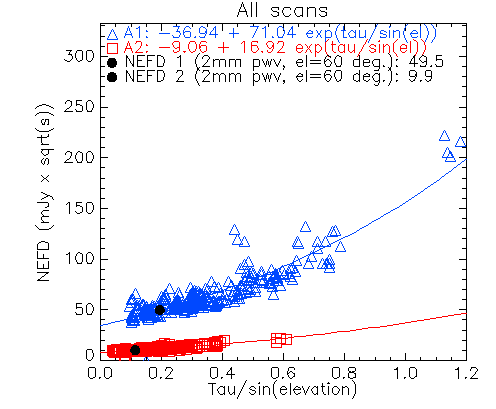
\includegraphics[clip, angle=0, scale =
%%   0.5]{Figures/NEFD_vs_tau_20170226s415_FXDC0C1_Jy_common_mode_kids_out.png}
%% 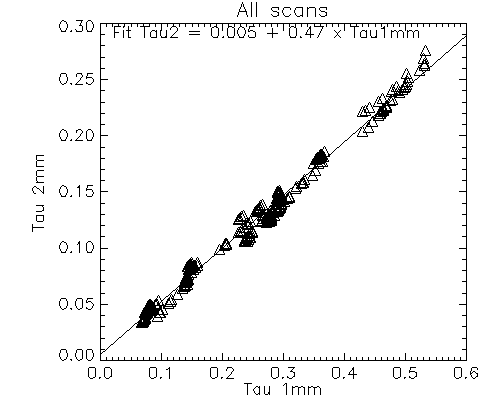
\includegraphics[clip, angle=0, scale =
%%   0.5]{Figures/tau1_tau2_20170226s415_FXDC0C1_GaussPhot_common_mode_kids_out.png}
%% \caption{}
%% \label{fig:fov}
%% \end{center}
%% \end{figure}

%  figure deplacee dans Opacity_checks.tex
%\begin{figure}
%\begin{center}
%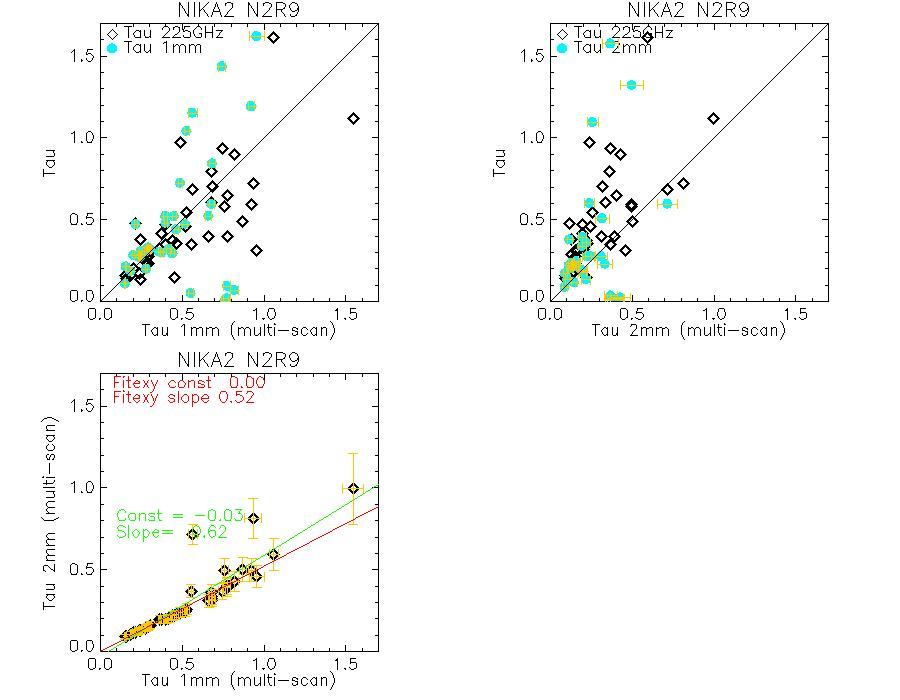
\includegraphics[clip, angle=0, scale = 0.5]{Figures/test_allskd_N2R9.jpg}
%\caption{{\bf Fix me : improve plot quality and plot only the 3rd one.}}
%\label{fig:test_allskd_N2R9}
%\end{center}
%\end{figure}

%\subsection{Opacity measurement consistency tests}

%{\bf copy from the 'Instru' paper}

\begin{figure}[ht]
\begin{center}
\includegraphics[scale=0.8]{Figures/test_allskd_N2R10v2commiss2.pdf}
\caption{Atmospheric opacity as measured from the NIKA2 data 
at 260 (top) and 150\,GHz (bottom) during N2R10
commissioning campaign. Each block of 40 KIDs gives an independent estimate of
the opacity value for each skydip scan (the integer abscissae). The block
number is the decimal value of the abscissae.
\label{fig:taumeas_paper}}
\end{center}
\end{figure}

\begin{figure}[ht]
\begin{center}
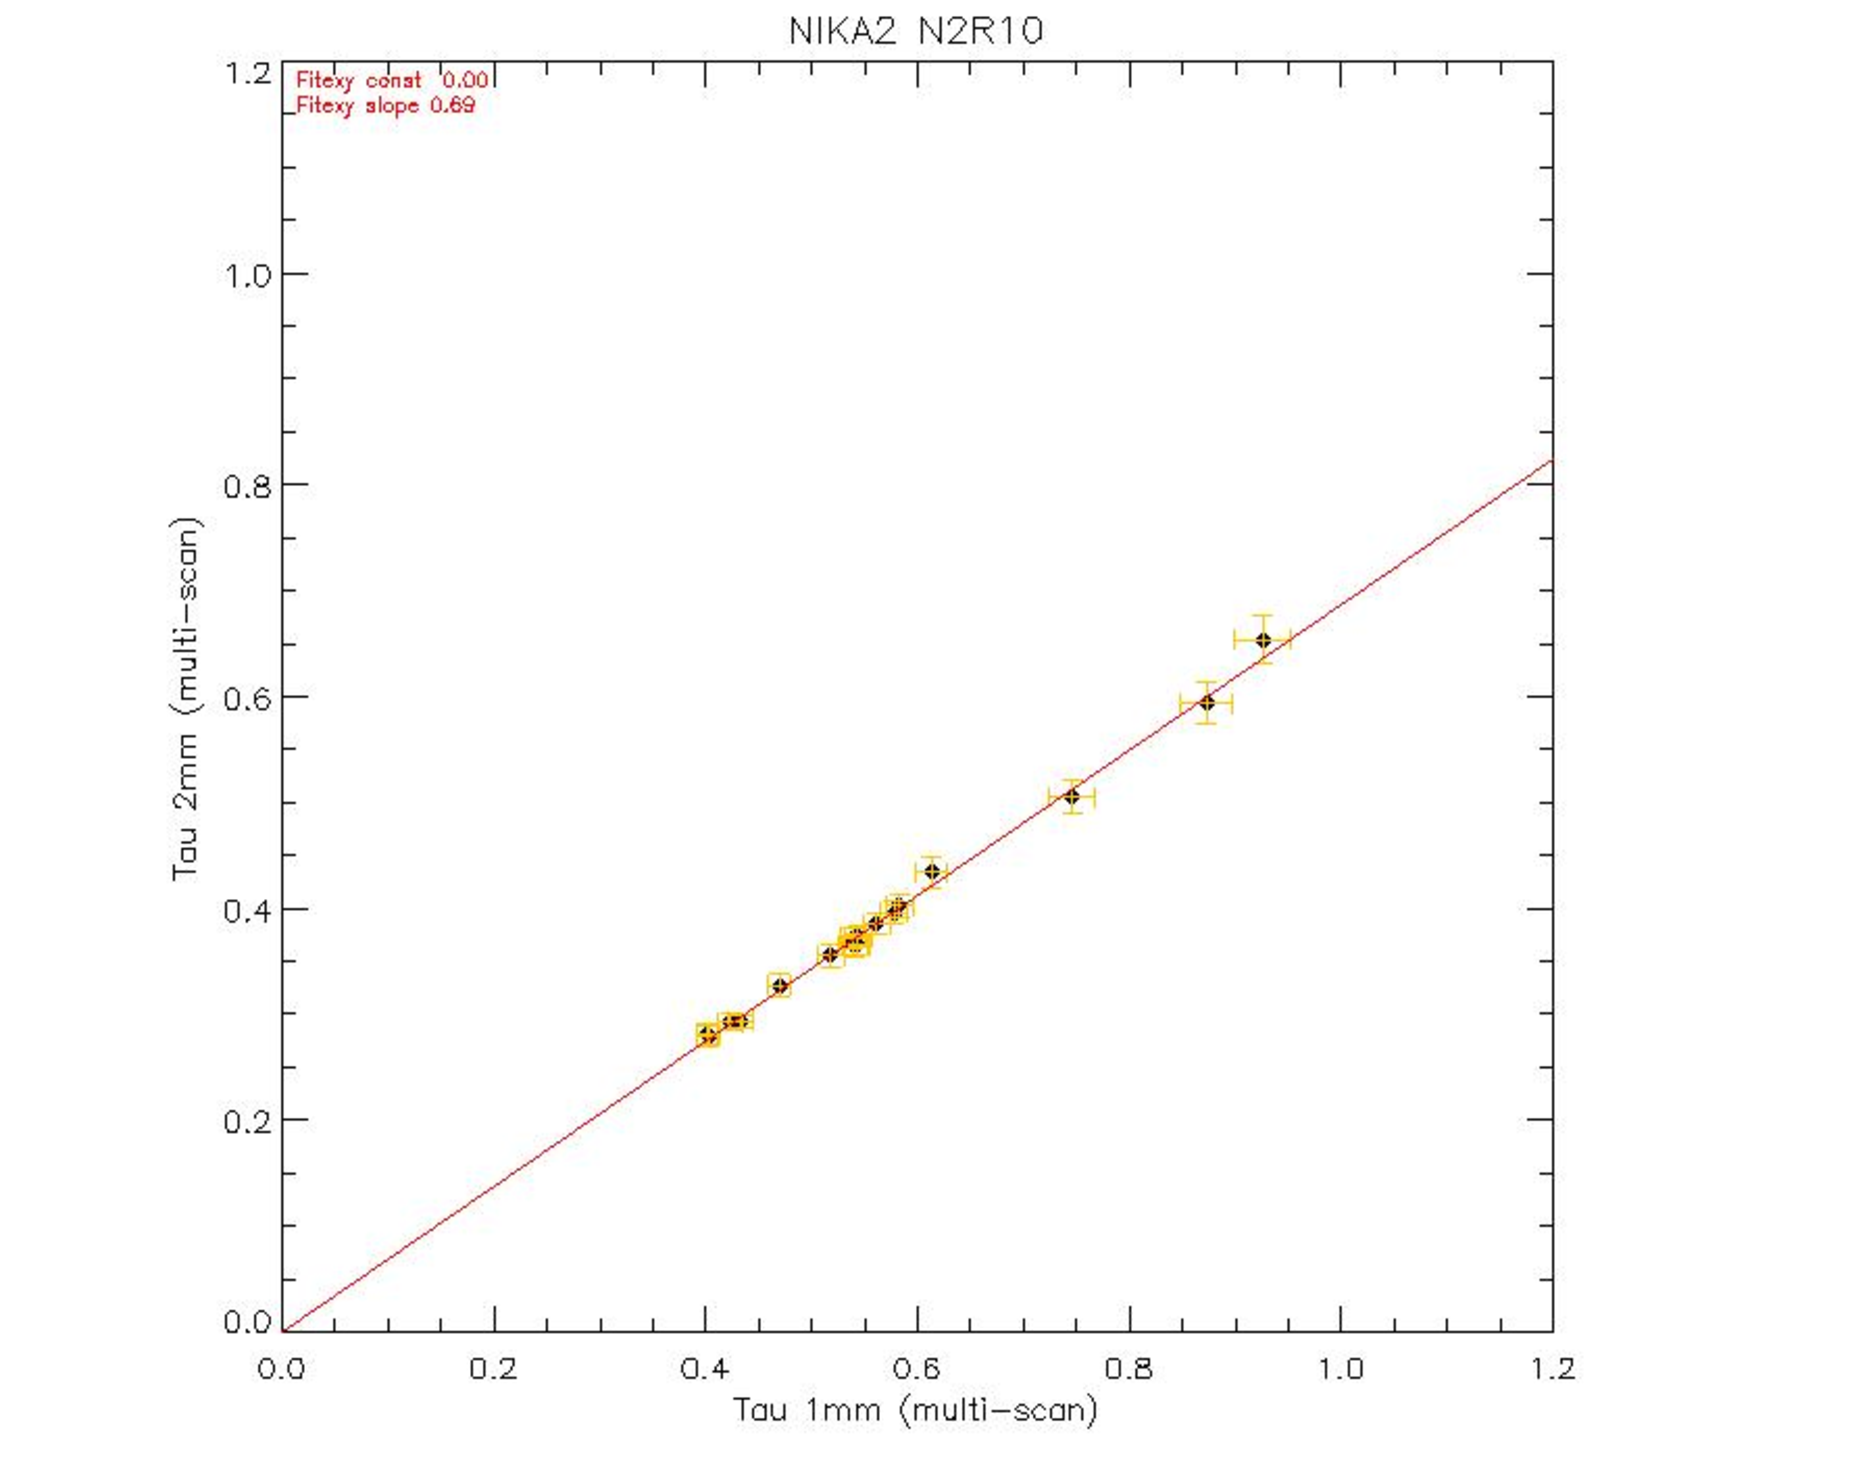
\includegraphics[scale=0.8]{Figures/test_allskd_N2R10v2commiss1.pdf}
\caption{Atmospheric opacity as measured from the NIKA2 data 
at 260 and 150\,GHz during N2R10
commissioning campaign. The error bars are in fact dispersion of the deduced
opacities between blocks of 40 KIDs.
\label{fig:taumeas_paper}}
\end{center}
\end{figure}

We observe that the skydip-fitted $\tau$ values are, as expected, common
between different detectors of the same array (the two 1mm arrays show
slightly different values). By comparing the results of different skydips, we
have verified experimentally that the coefficients $C_0$, $C_1$ are stable,
within the fit errors, on very long time scales within a cooldown cycle. The
coefficients can thus be applied to the whole observing campaign in order to
recover the opacity of each scan.


% \noindent {\bf FM : a figure would help to convince the reader that it is stable on lng time
% scale, which is a key point.}\\ FXD: I will do that figure


\begin{figure}[ht]
\begin{center}
\includegraphics[scale=0.8]{../../Paper_NIKA2_Technical/opacity_evol_run22.pdf}
\caption{Atmospheric opacity as measured from the IRAM 225\,GHz taumeter
(cyan), and from the NIKA2 data at 150 (red) and 260\,GHz (blue) during N2R9
commissioning campaign (Feb. 2017). We stress the fact that the IRAM 225\,GHz
taumeter data is not used for the atmospheric correction and is plotted here
just for comparison.
  \label{fig:taumeas_paper}}
\end{center}
\end{figure}


\begin{figure}[ht]
\begin{center}
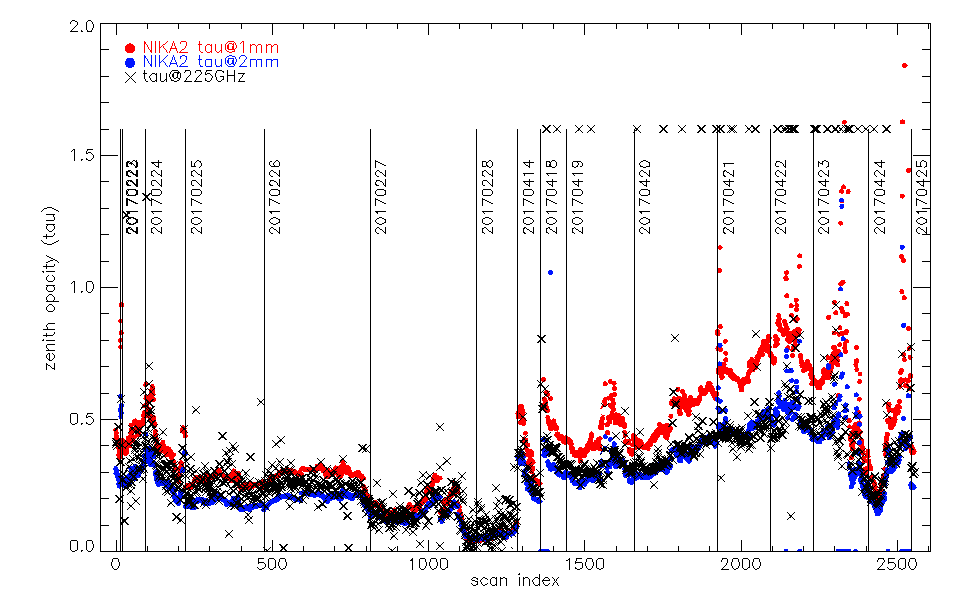
\includegraphics[width=\linewidth]{Figures/opacity_vs_index_N2R9_N2R10.png}
\caption{Atmospheric opacity as measured from the IRAM 225\,GHz
  taumeter (black crosses), and from the NIKA2 data at 150 (red) and 260\,GHz (blue) during 
  N2R9 and N2R10 commissioning campaigns.  We stress the fact that the IRAM 225\,GHz taumeter data is not used for the atmospheric correction and is plotted here just for comparison.
  \label{fig:taumeas}}
\end{center}
\end{figure}


In Fig.~\ref{fig:taumeas} {\bf(and Fig.~\ref{fig:taumeas_paper} of
  \ref{NIKA2-Tech}) } we present the evolution of the NIKA2 in-band
opacities for all the 'OTF' scans (about 1300 scans per runs) of the
N2R9 run held in February and the N2R10 run in April 2017. These are
compared to the IRAM tau-meter values. We observe an agreement on the global trend between the IRAM tau-meter opacity
(225 GHz) and the NIKA2 values. These latter show, however,
a smaller dispersion (less than one percent).
% {\bf FM : how small ?}.


We find an average ratio between the 150 GHz and the 260 GHz NIKA2 values of
about 0.6, a bit higher than ATM model expectations. We notice however that
the 150 GHz-to-260 GHz opacity ratio varies significantly for opacities (at
150 GHz) below 0.2. This effect is likely to be linked to an $O_2$ atmospheric
line which becomes saturated or to some spillover at 2mm. This point is,
however, still under investigation.''


% \noindent {\bf FM : a figure of the ratio of taus would be useful. It should be compared with  
% Fig. \ref{thopacities}, which should appear in this section ...}
% FXD: figure above gives the measured ratio. 


\begin{figure}[ht]
\begin{center}
  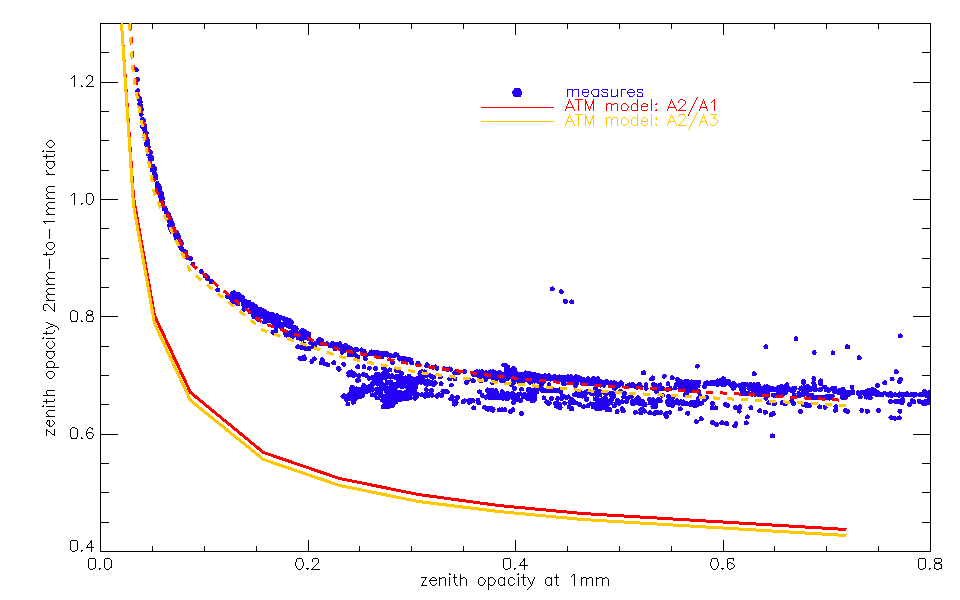
\includegraphics[width=0.65\textwidth]{Figures/opacity_tau1_tau2_ratio_N2R9_N2R10.png}
  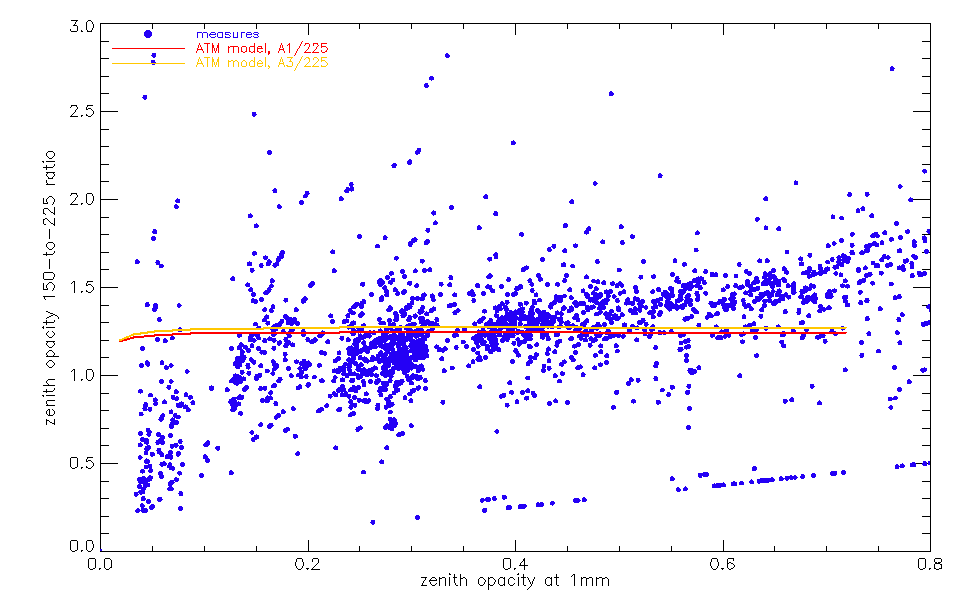
\includegraphics[width=0.65\textwidth]{Figures/opacity_tau1_tau225_ratio_N2R9_N2R10.png}
  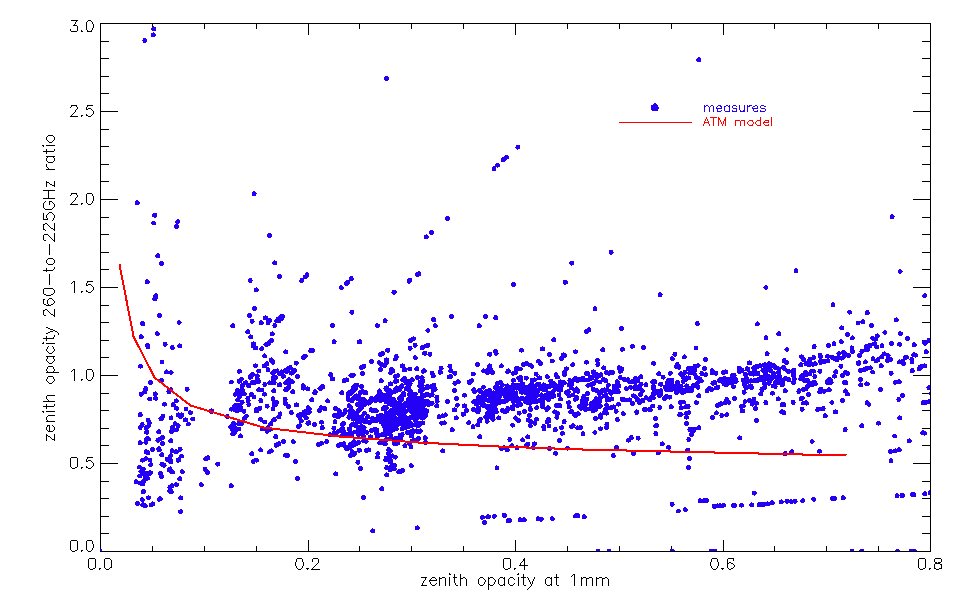
\includegraphics[width=0.65\textwidth]{Figures/opacity_tau2_tau225_ratio_N2R9_N2R10.png}
\caption{Ratios between the 150 GHz and the 260 GHz NIKA2 zenith opacity
estimates and between the NIKA2 $\tau$ and the IRAM taumeter
values. The expectation values derived for NIKA2 bands
using the ATM model described in \ref{Pardo2002} are shown for
comparison (red and orange curves).}
  \label{fig:opacity_ratios}
\end{center}
\end{figure}

\begin{figure}[ht]
\begin{center}
  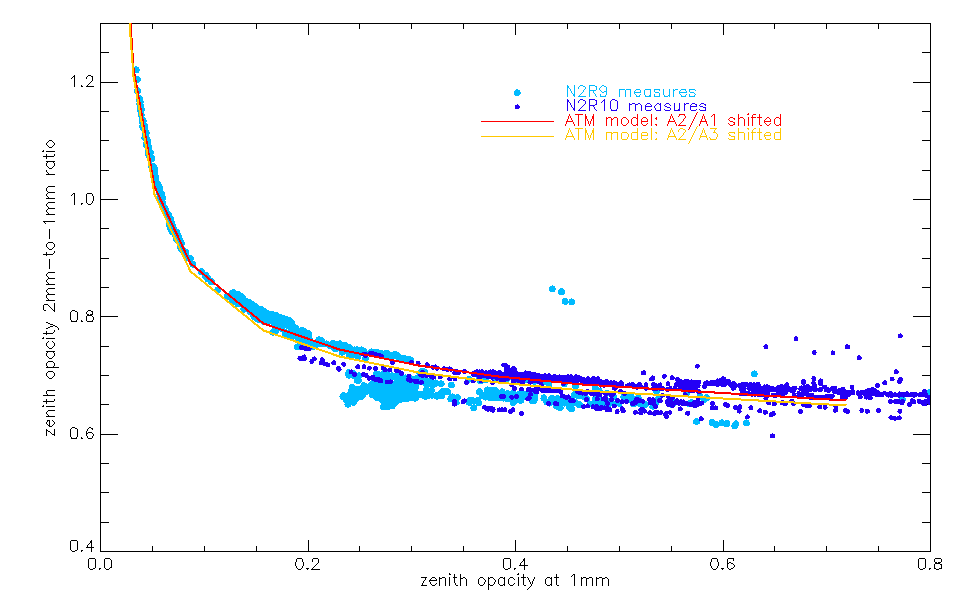
\includegraphics[width=0.8\textwidth]{Figures/opacity_tau1_tau2_byrun_ratio_N2R9_N2R10.png}
  \caption{Ratio between the 150 GHz and the 260 GHz NIKA2 zenith opacity
estimates. The expectation values derived for NIKA2 bands
using the ATM model described in \ref{Pardo2002} are shown for
comparison (red and orange curves). The observed NIKA2 opacity ratio
has a smooth, consistent behaviour over the overall probed opacity range,
and very few outlier estimates are seen although no scan selection has
been performed (out from discarding the dark tests). Also remarkable
is the consistency between estimates obtained during two campaigns
held two months apart in different weather conditions (good to average
during N2R9 and poor and often hightly unstable conditions during
N2R10). Some sub-structures are seen in the opacity ratio, which are
under investigations. They can have several origins (telescope cabin
temperature variation, variation of the $0_2$ fraction, atmospheric
temperature variation, internal temperature variations, etc).  
  }
  \label{fig:opacity_ratio_perrun}
\end{center}
\end{figure}


\begin{figure}[ht]
\begin{center}
  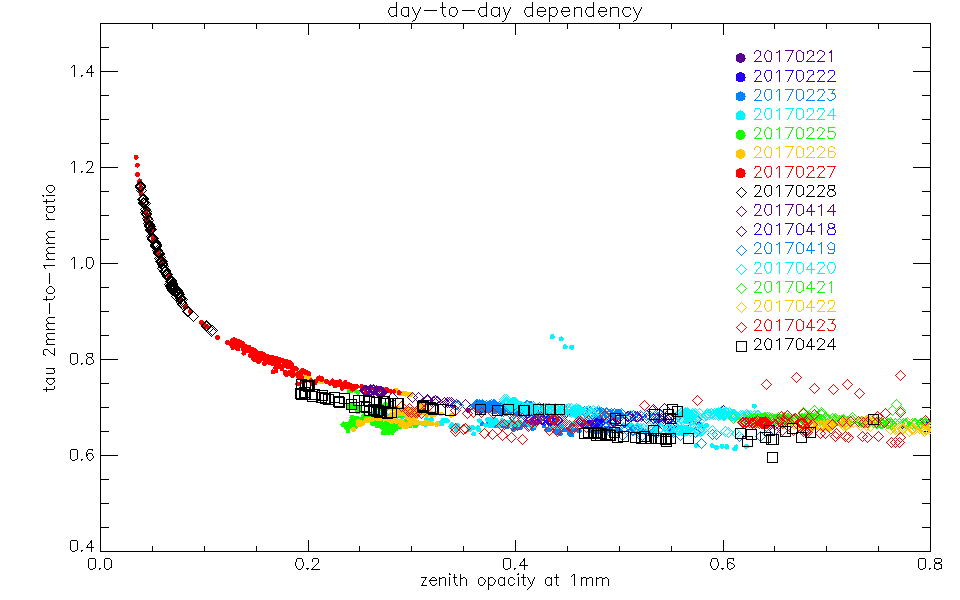
\includegraphics[width=0.8\textwidth]{Figures/opacity_tau1_tau2_ratio_perday_N2R9_N2R10.png}
  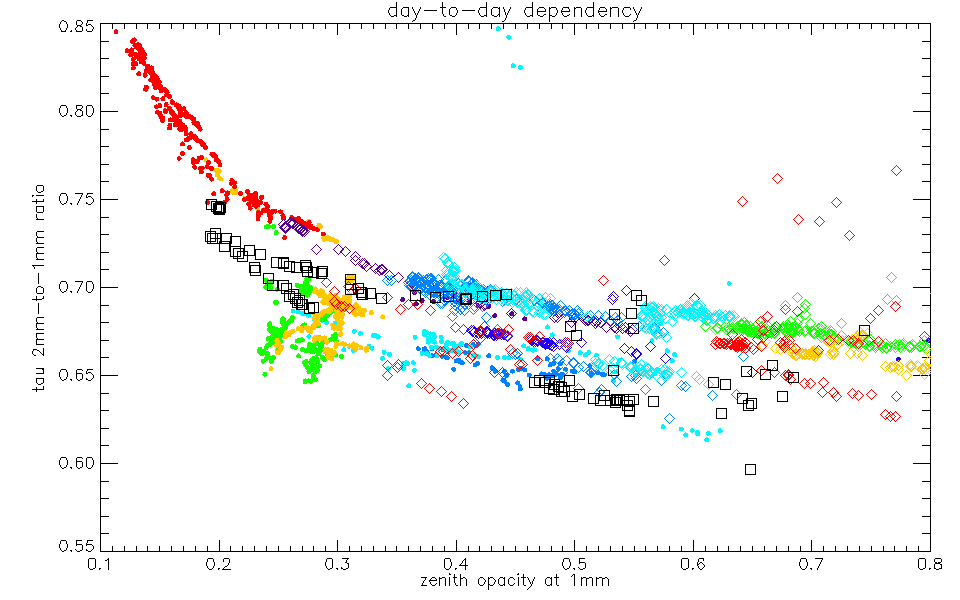
\includegraphics[width=0.8\textwidth]{Figures/opacity_tau1_tau2_ratio_perday_zoom_N2R9_N2R10.png}
  \caption{Ratio between the 150 GHz and the 260 GHz NIKA2 zenith
    opacity estimates. The 4 outlier estimates on February, 24 (in
    cyan) correspond to a test using the external
    calibrator. Different regimes are seen on the 25th and 26th of
    February, while the weather conditions were too unstable to allow
    the astronomer team to focus.
  }
  \label{fig:opacity_ratio_perday}
\end{center}
\end{figure}


\begin{figure}[ht]
\begin{center}
  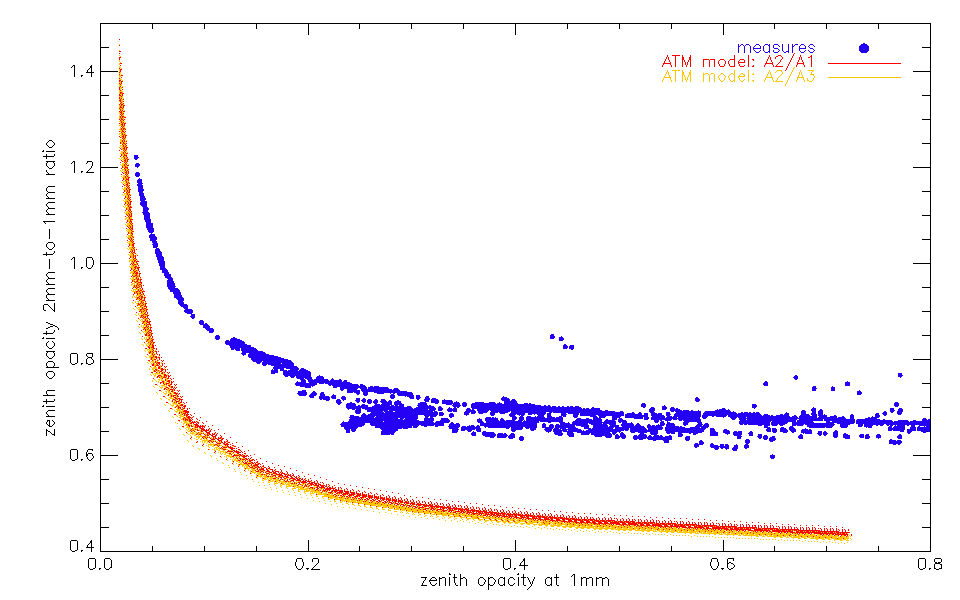
\includegraphics[width=0.8\textwidth]{Figures/opacity_tau1_tau2_ratio_bperror10pc_N2R9_N2R10.png}
  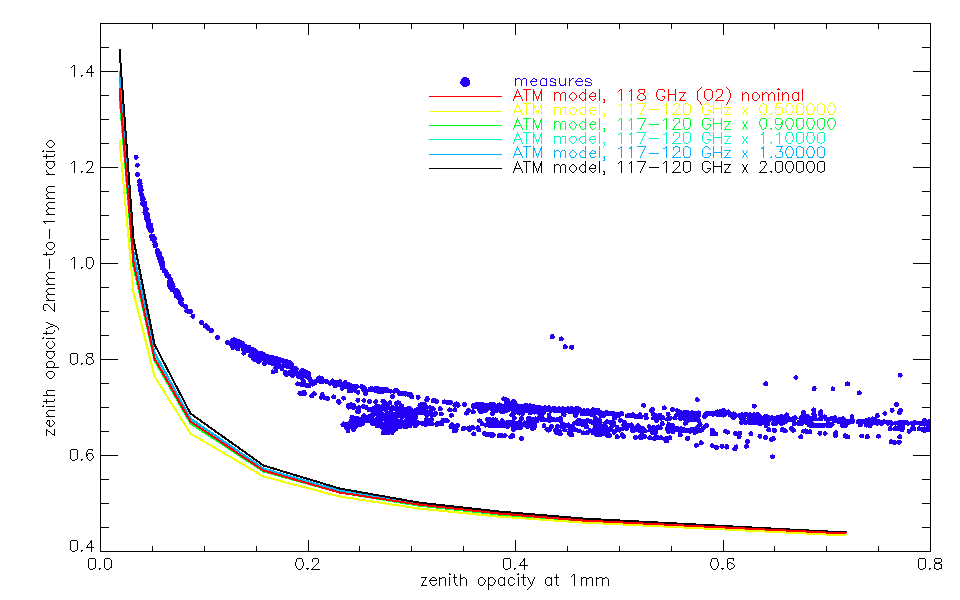
\includegraphics[width=0.8\textwidth]{Figures/opacity_tau1_tau2_ratio_o2fraction_N2R9_N2R10.png}
\caption{Uncertainty of NIKA2 $\tau$ values. Upper panel: The impact
  of the NIKA2 transmission measurement uncertainties is illustrated
  using a very pessimistic relative uncertainty of $10\%$ (instead of
  the more realistic $1\%$ errors). Lower panel: The impact of the
uncertainty on the atmospheric absorption around $118\, \rm{GHz}$, due
to the lack of precise knowledge of the fraction of oxygene in the
atmosphere. The nominal absorption predicted by the ATM model is
modified by a factor from 0.5 to 2 in the $117-120\, \rm{GHz}$
frequency band, where the $0_2$ contributions largely dominates the
water vapor ones. }
  \label{fig:opacity_errors}
\end{center}
\end{figure}

\begin{figure}[ht]
\begin{center}
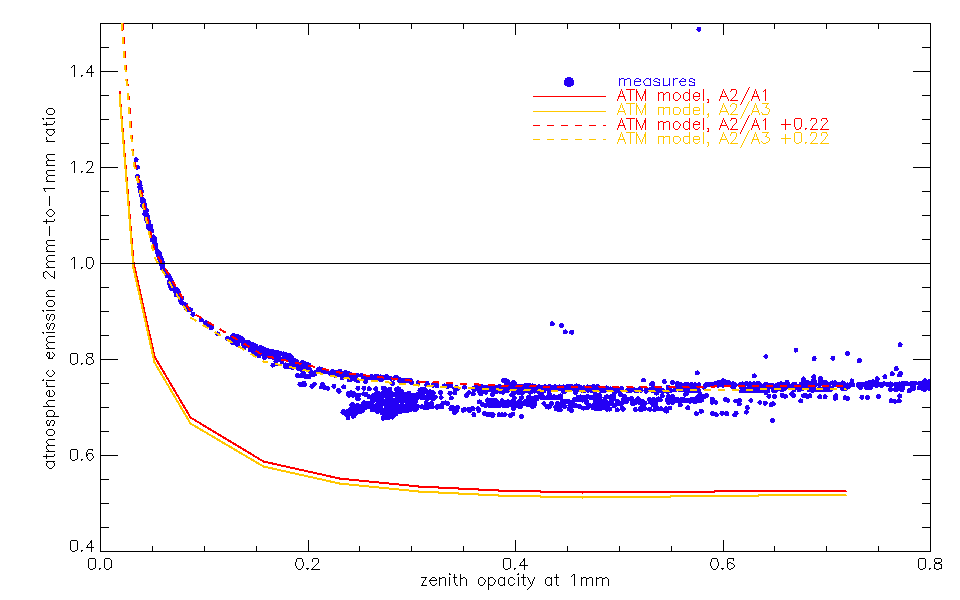
\includegraphics[width=0.9\textwidth]{Figures/opacity_tau1_tau2_emissionratio_N2R9_N2R10.png}
\caption{Ratio of the atmospheric emission in NIKA2 bands defined as
  in Eq.~\ref{eq:opacity_emission_ratio}, compared with the ATM-model
  predicted ratio calculated as in Eq.~\ref{eq:opacity_emission_ratio_model}}
  \label{fig:opacity_emission}
\end{center}
\end{figure}

The ratios between the 150 GHz and the 260 GHz NIKA2 zenith opacity
estimates, quoted $\tau_{2mm}$ and $\tau_{1mm}$ , and
between the NIKA2 $\tau$ and the IRAM taumeter values are presented in
Fig.~\ref{opacity_ratios}, along with the expectation values derived for NIKA2 bands
using the ATM model described in \ref{Pardo2002}. Namely, these
predicted values $\tau^{th}$ are calculated from the ATM-model
atmospheric zenith opacity $\tau^{ATM}$ using:  
\begin{equation}
  \tau^{th}_{A_i} = - \ln{\frac{\int e^{-\tau^{ATM}(\nu)}
      T_{A_i}(\nu) d\nu}{ \int T_{A_i}(\nu) d\nu}},
\end{equation}

where the NIKA2 bandpasses $T_{A_i}$ for arrays $A_i$, $i=1, 2, 3$, are the Martin-Pupplet reference transmissions
corrected by a Rayleigh-Jeans term  $T'_{A_i}(\nu) /
\left( \frac{\nu}{\nu_0}\right)^2$. 

In Fig.~\ref{fig:opacity_emission}, we
show the ratio of the atmospheric emission in NIKA2 bands defined as:
\begin{equation}
  R_{\rm{atm}} = \frac{1-e^{-\tau_{2mm}}}{1-e^{-\tau_{1mm}}}.
    \label{eq:opacity_emission_ratio}
\end{equation}

It is compared with the ATM-model predicted ratio
\begin{equation}
  R_{\rm{atm}}^{th} = \frac{\int (1 - e^{-\tau^{\rm{ATM}}}) T_{A_2}(\nu) d\nu }{\int T_{A_2}(\nu) d\nu} / \frac{\int (1 -
      e^{-\tau^{\rm{ATM}}}) T_{A_{1}}(\nu) d\nu }{\int T_{A_1}(\nu)
        d\nu} .
      \label{eq:opacity_emission_ratio_model}
\end{equation}

In Fig.~\ref{fig:opacity_errors}, we investigate different effects that can impact the precision with
which the zenith opacities are determined: the upper panel shows the
expected dispersion in the NIKA2 $\tau$ values coming from the transmission
measurement uncertainties: to higlight this effect, we consider a very
pessimistic relative uncertainty of $10\%$ (whereas $1\%$ would have
been a more realistic value), and the lower panel shows the impact of the
uncertainty on the fraction of oxygene in the atmosphere, which mainly 
translates in an uncertainty on the atmospheric absorption around
$118\, \rm{GHz}$: the nominal absorption predicted by the ATM model is
modified by a factor from 0.5 to 2 in the $117-120\, \rm{GHz}$
frequency band, where the $0_2$ contributions largely dominates the
water vapor ones. 



We have compared $C_0$ values, the resonance frequency at zero atmosphere,
between different runs. It appears to vary in a systematic manner. For example
we have compared N2R6 and N2R7. The change of frequencies when converted to
temperature (with $c_1$) is of about $25$ and $86$~K at 1 and $2$~mm. This
cannot be a real change of the background. Translated back by a median value
of $c_1$ ($=2500$ and $1500$~Hz/K at 1 and 2 mm), we obtain a 62.5 and 128 kHz
median downward shift of all resonant frequencies between N2R6 (October 2016)
and N2R7 (December 2016). The likely explanation is that of a slight ageing of
the KIDs. A single monolayer of oxyde could be enough to produce the downward
shift.



% LP: copie de l'intro de Xavier
In NIKA2, the opacity is measured via a total-power technique, which was
successfully tested with NIKA. The details of this technique and its agreement
with the Atmospheric Transmission at Microwaves (ATM) model
(\cite{2001IEEE....49.1683C}) are described in \cite{Catalano:2014nml}. The
underlying idea is to replace the opacity, usually delivered by the resident
IRAM tau-meter that performs elevation scans at a fixed azimuth and is
operating at 225\,GHz, by a measurement that uses the NIKA2 instrument itself
as a tau-meter. Using this procedure we can directly derive an opacity
integrated in the NIKA2 very bandpasses and in the same line-of-sight of the
source in the considered map. For that purpose, we assume that the resonance
frequency of each KID varies linearly with the total power. First, we have to
calibrate the relationship between total power and opacity. Then we can use
that calibration to measure the opacity during a given scan.
% fin copie


%----------------------------------------------------------------------------------------
%	skydip-based Method
%----------------------------------------------------------------------------------------
\subsection{Skydip-based method}
\label{se:skydip-method}

For each KID $k$, the absolute value of the resonance frequency
$f_{tone}^k$ moves with the atmospheric load according to

\begin{equation}
\ftone^k  = C_0^k - C_1^k T_{atm}[1-e^{-\tau/\sin\delta}]
\label{eq:skydip}
\end{equation}

%FXD corrected 
%{\bf LP: pourquoi signe plus alors qu'on utilise un signe moins dans
%  Eq. 2 du papier instru ?}

where $C_0^k$ is a constant equal to the resonance
frequency at zero opacity, $C_1^k$ is the calibration conversion
factor in kHz$/$K, $T_{atm}$ is the equivalent temperature
of the atmosphere (taken as a constant at 270~K), $\tau$ the zenith
opacity and $\delta$ the average elevation of the telescope.
By assuming a homogeneous plane-parallel atmosphere, the airmass $x$ is defined from the
elevation as $x = \left(\sin\delta\right)^{-1}$. 

The coefficients $C_0^k$ and $C_1^k$ are expected to be constant in
time within at least a cooldown cycle, and are determined using a {\tt
skydip} procedure. This consists in moving the telescope in elevation
step by step and monitoring, for each kid, the evolution of $\ftone^k$
versus the air mass and to fit the zenith opacity $\tau$ and $C_0^k$
and $C_1^k$. This process is realised by performing a skydip scan, as
defined in~Sect.~\ref{se:skydip}. The acquisition time spend on each
elevation step, wich is of about twenty seconds, is chosen to reduce
the error in the determination of $\ftone^k$.

All skydips, obtained under various opacity
conditions, are analysed together to break the degeneracies between
the opacity and the responsivity ($C_1^k$). The procedure has two steps.
First, all the skydips are analysed individually to simply extract
$\ftone^k$ for each stable elevation. Secondly, a simultaneous fit is done
for all 
parameters ($\tau$, $C_0^k$ and $C_1^k$.)
Error bars on $\tau$ are estimated by doing
this procedure on blocks of 40 kids only and getting a dispersion on the
resulting $\tau$ from the different blocks. Usually the dispersion comes out as
$4\times 10^{-3}$ at 1 mm and $1\times 10^{-3}$ at 2 mm. Once the $\tau$ values
are estimated for each skydip (as the average over the blocks), we compute
(while fixing $\tau$) the $C_0$ and $C_1$ final values for each KID. We thus
retrieve the coefficients of all the KIDs even though some of them could not
contribute to the $\tau$ determination.

This procedure consists thus in fitting a couple of paramaters ($C_0$,
$C_1$) for each of the several thousand valid KIDs. This requires to
have on hands a sizable amount of skydip scans -- typically ten to
twenty -- that i) span the whole opacity range and ii) avoid hightly
perturbated atmosphere to met the plane-parallel atmosphere
assumption. To that aim, we recommand to perform a skydip scan twice a
day during a scientific campagn. Then during the ($C_0$, $C_1$)
determination process, the skydip scan are thoroughtly selected.

   
\subsection{Skydip selection}


\begin{figure}[p]
\begin{center}
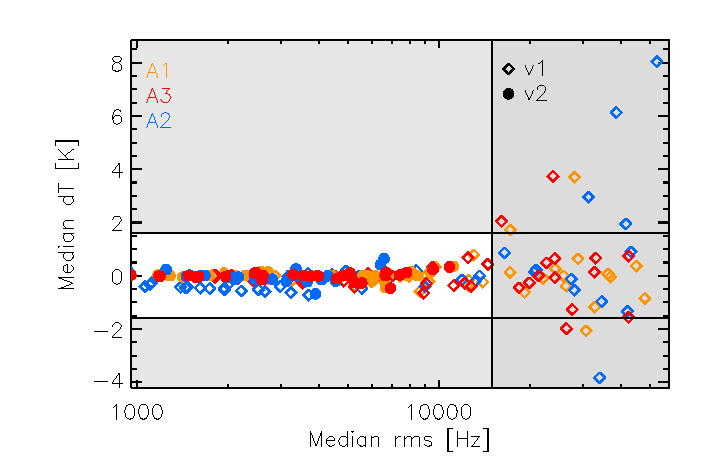
\includegraphics[clip=true,width=0.9\linewidth]{Figures/Opacity/plot_skydip_selection_two_crit.pdf}
\label{fig:skydip_selection}
\caption{N2R9 skydip scan selection. Median dT quality-fit criterion is plotted in fonction of Median rms criterion for each skydip scans of the N2R9 campaign and for the three arrays. Both criteria are nicely correlated. Empty diamonds show the results of the first iteration of the skydip coefficient estimation, whereas filled circled show the second iteration, for which only the skydips that met both fit-quality criteria are included. After the second iteration, all the remaining skydips met the criteria.}
\end{center}
\end{figure}

For each skydip scan and for each bunch of 40 KIDs, we compute the
difference between the measured KID resonance frequency and the model
given in Eq.~\ref{eq:skydip} taken at the best-fit values of the
($C_0$, $C_1$) parameters. Then we determine two indicators
of the fit quality per skydip. First, the standard deviation of the
measure-to-model difference is calculated over all the KIDs in a
bunch. For each skydip, we evaluate the median rms, which is the
median over the KID bunches of the standard deviation per bunch, given
in Hz. Secondly, for each scan, we compute the average
measure-to-model difference of each KID $k$, labelled $dT_k$, which is
then converted from Hertz to Kelvin using the $C_1$ parameter of the
KID $k$. Median $dT$ is the median of $dT_k$ over all the KID of an
array. With these two indicators in hands, we discard the skydip scans
that are noisy or that yield a poor fit by applying the selection
criteria

\begin{itemize}
\item Median $\rm{rms} < 1.5 \times 10^{4}~\rm{Hz}$
\item Median $dT < 1.6~\rm{K}$
\end{itemize}

The threshold values have been determined using the set of 44 skydip
scans of N2R9. The Median rms cut corresponds to twice the median of
this quantity per skydip scan, whereas the Median $dT$ cut is twice
the standard deviation of Median $dT$ over the skydips. N2R9 skydip
scan selection is illustrated in Fig.~\ref{fig:skydip_selection}, in
which the agreement between the two fit-quality criteria is clearly
seen. The ($C_0$, $C_1$) estimation proceeds in two steps: first the
parameters are estimated using all the available skydip scan for a
given campaign, then the estimation is re-iterated using the only
skydip scans that met the fit-quality criteria. After the second
iteration, we check that no extra skydip outlier are left, as shown by
the 'v2' label data points in Fig.~\ref{fig:skydip_selection}.


We test the stability of the ($C_0$, $C_1$) parameters against the exact choice of the selection criteria.  

\addparag{stability against the skydip scan selection + FIG}

At 1mm, we find about {\color{red} $[$TBC$]$  $10\%$} opacity variation from very inclusive to very aggressive selections. However, at 2mm, this scatter reachs about {\color{red} $[$TBC$]$  $30\%$} relative uncertainties.


We conclude that opacities at 1mm can be reliably estimated from a series of skydip scans using the (C0, C1) model. By contrast, for the 2mm opacities, a skydip-based method is not stable enough against the skydip selection. Thus, we adopt an hybrid approach. 

\subsection{The hybrid method}

The hybrid method comprizes two-steps: i) first the 1mm opacities,
that are $\tau_{A1}$ and $\tau_{A3}$, are determined using the skydip
method described in Sect.~\ref{se:skydip-method}, ii) then the 2mm
opacity $\tau_{A2}$ is extrapolated from the 1mm ones using a modified
ATM model. Namely, for the second step, we perform:

\begin{equation}
\tau_{A2} = \left( \left.\frac{\tau_{A2}^{\rm{ATM}}}{\tau_{A3}^{\rm{ATM}}}\right\vert_{\tau_{A3}} + \alpha \right) \tau_{A3},
\end{equation}

 where $\alpha$ is an offset, which are estimated from the observations themselves, and the ratio is the predicted zenith opacity ratio for A2 and A3 frequency bands using the ATM model described in \ref{Pardo2002} and taken at the measured A3 zenith opacity. The zenith opacity expectations for the array $A_i$ is
\begin{equation}
  \tau^{\rm{ATM}}_{A_i} = - \ln{\frac{\int e^{-\tau^{ATM}(\nu)} T_{A_i}(\nu) d\nu}{ \int T_{A_i}(\nu) d\nu}},
\end{equation}
where the bandpasses $T_{A_i}$ for arrays $A_i$, $i=1, 2, 3$, are the Martin-Pupplet reference transmissions
corrected by a Rayleigh-Jeans term  $T'_{A_i}(\nu) / \left( \frac{\nu}{\nu_0}\right)^2$. 

We observe that the measured \emph{shape} of the measured opacity ratio is well described by the ATM expectations whereas its \emph{amplitude} is too low by an offset $\alpha$, which we dertermine using a data-driven approach. We estimate $\alpha$ as the offset that ensures a stability of the A2 flux over the whole opacity span.  

\addparag{$\alpha$ fit + FIG}





%----------------------------------------------------------------------------------------
%	Tests
%----------------------------------------------------------------------------------------
\subsection{Baseline opacity measurements}

%{\bf copy from the 'Instru' paper}

%\begin{figure}[ht]
%\begin{center}
%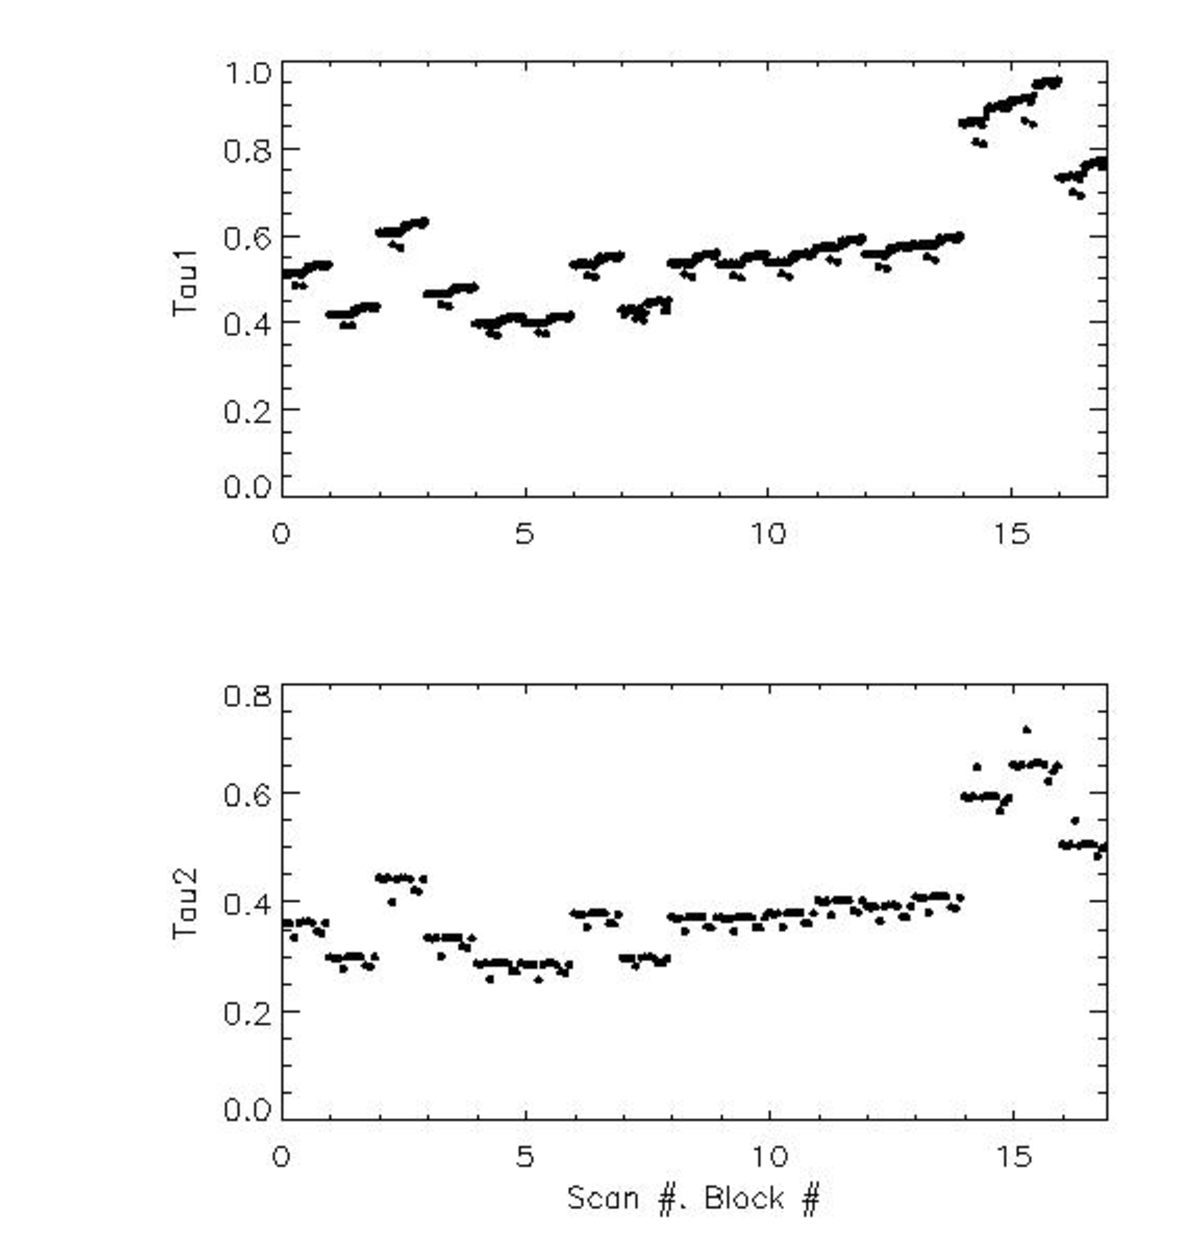
\includegraphics[scale=0.8]{Figures/test_allskd_N2R10v3commiss2.pdf}
%\caption{Atmospheric opacity as measured from the NIKA2 data 
%at 260 (top) and 150\,GHz (bottom) during N2R10
%commissioning campaign. Each block of 40 KIDs gives an independent estimate of
%the opacity value for each skydip scan (the integer abscissae). The block
%number is the decimal value of the abscissae.
%\label{fig:taumeas_paper}}
%\end{center}
%\end{figure}

%\begin{figure}[ht]
%\begin{center}
%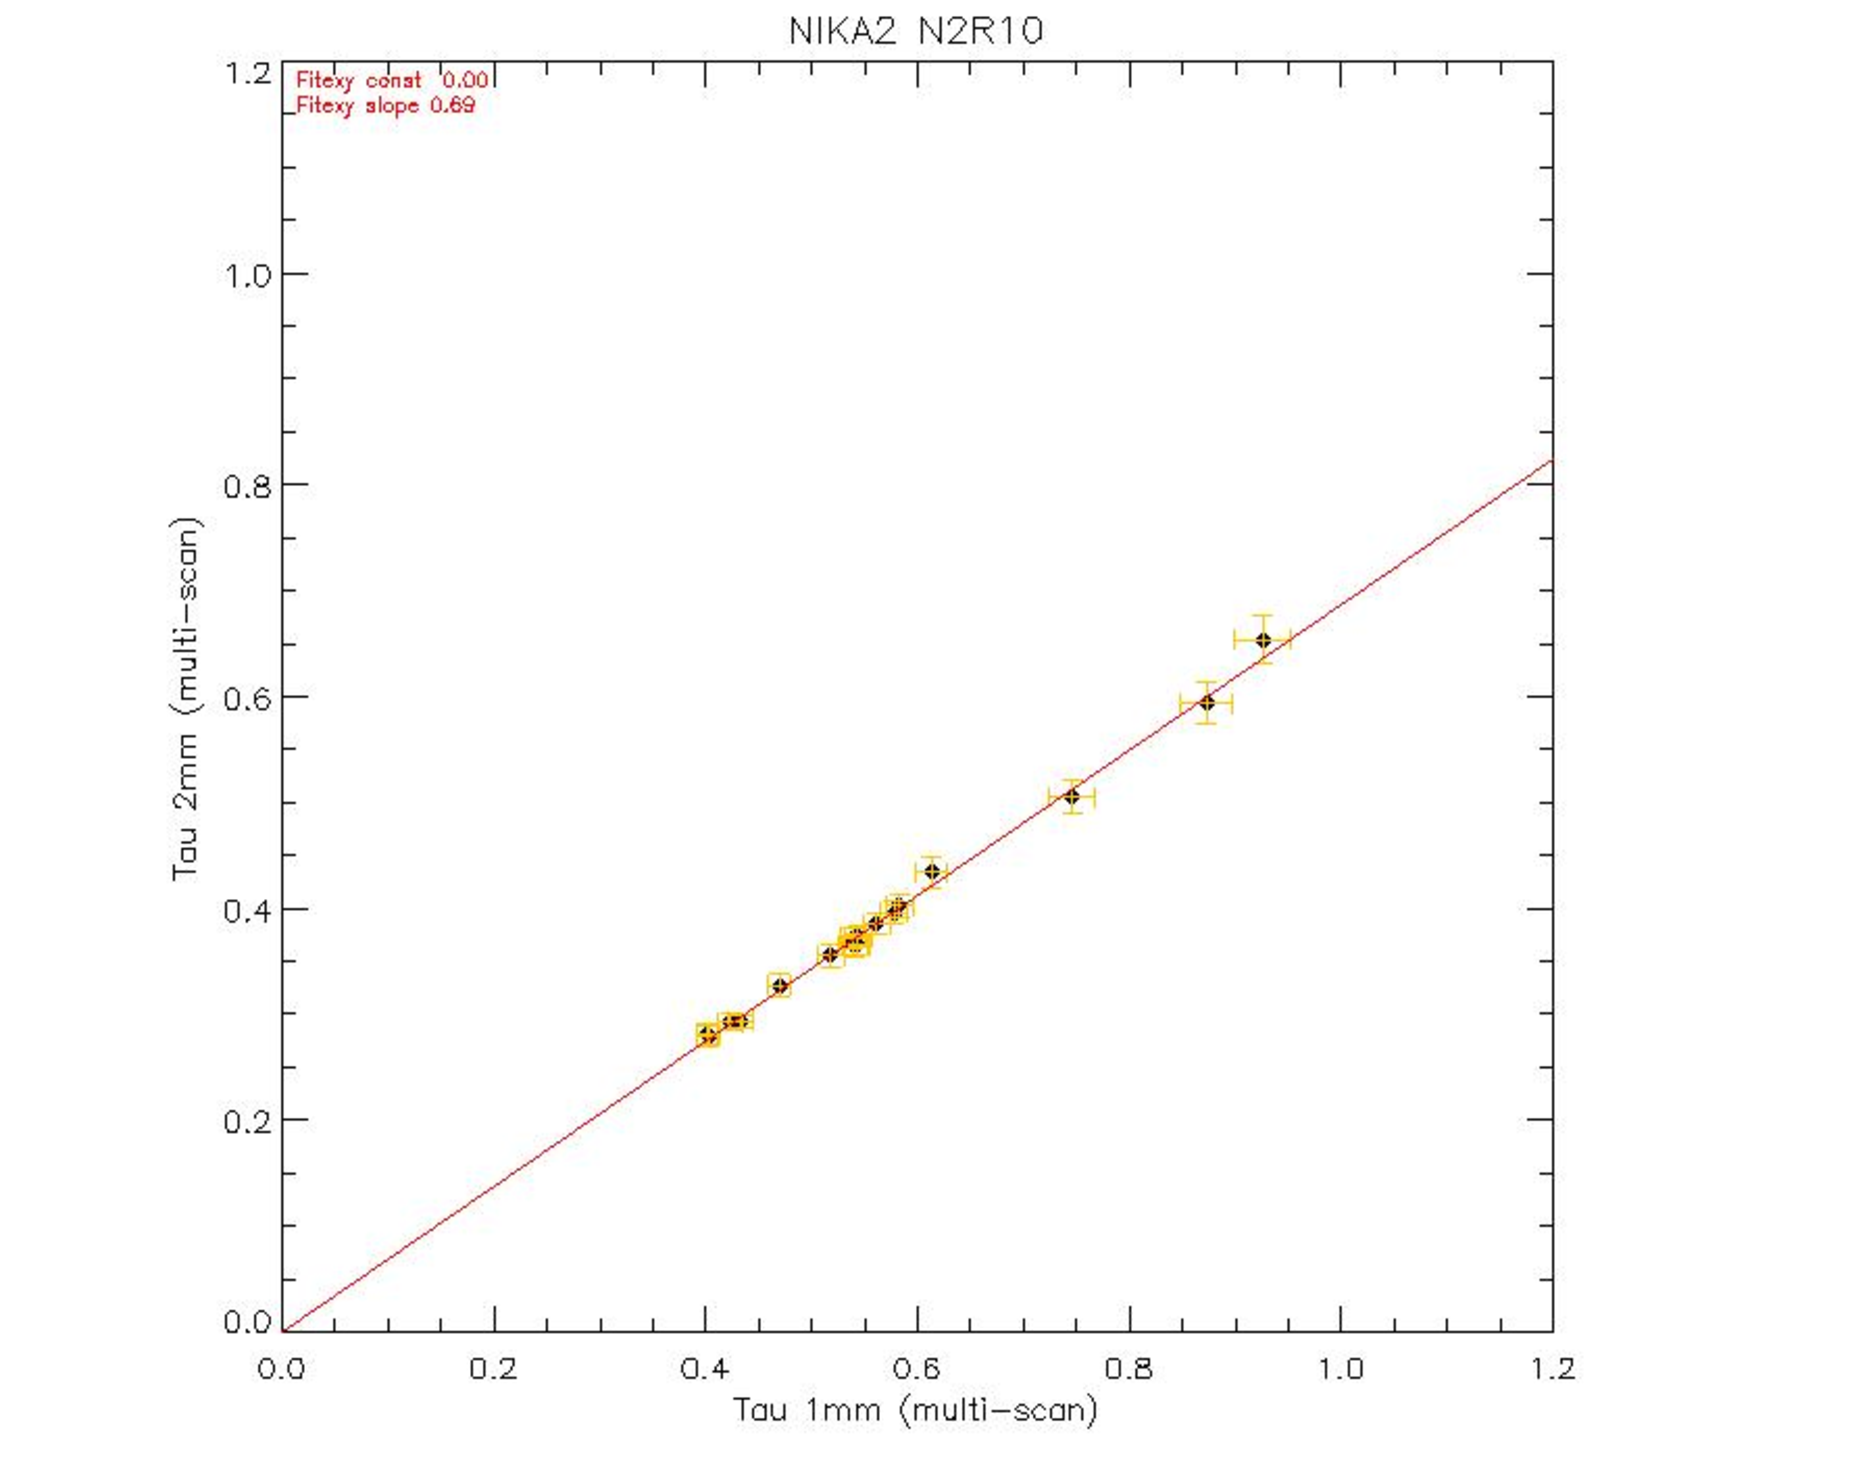
\includegraphics[scale=0.8]{Figures/test_allskd_N2R10v2commiss1.pdf}
%\caption{Atmospheric opacity as measured from the NIKA2 data 
%at 260 and 150\,GHz during N2R10
%commissioning campaign. The error bars are in fact dispersion of the deduced
%opacities between blocks of 40 KIDs.
%\label{fig:taumeas_paper}}
%\end{center}
%\end{figure}

We observe that the skydip-fitted $\tau$ values are, as expected, common
between different detectors of the same array. By comparing the results of different skydips, we
have verified experimentally that the coefficients $C_0$, $C_1$ are stable,
within the fit errors, on very long time scales within a cooldown cycle. The
coefficients can thus be applied to the whole observing campaign in order to
recover the opacity of each scan.


% \noindent {\bf FM : a figure would help to convince the reader that it is stable on lng time
% scale, which is a key point.}\\ FXD: I will do that figure


\begin{figure}[ht]
\begin{center}
\includegraphics[scale=0.8]{../../../Paper_NIKA2_Technical/opacity_evol_run22.pdf}
\caption{Atmospheric opacity as measured from the IRAM 225\,GHz taumeter
(cyan), and from the NIKA2 data at 150 (red) and 260\,GHz (blue) during N2R9
commissioning campaign (Feb. 2017). We stress the fact that the IRAM 225\,GHz
taumeter data is not used for the atmospheric correction and is plotted here
just for comparison.
  \label{fig:taumeas_paper}}
\end{center}
\end{figure}


\begin{figure}[ht]
\begin{center}
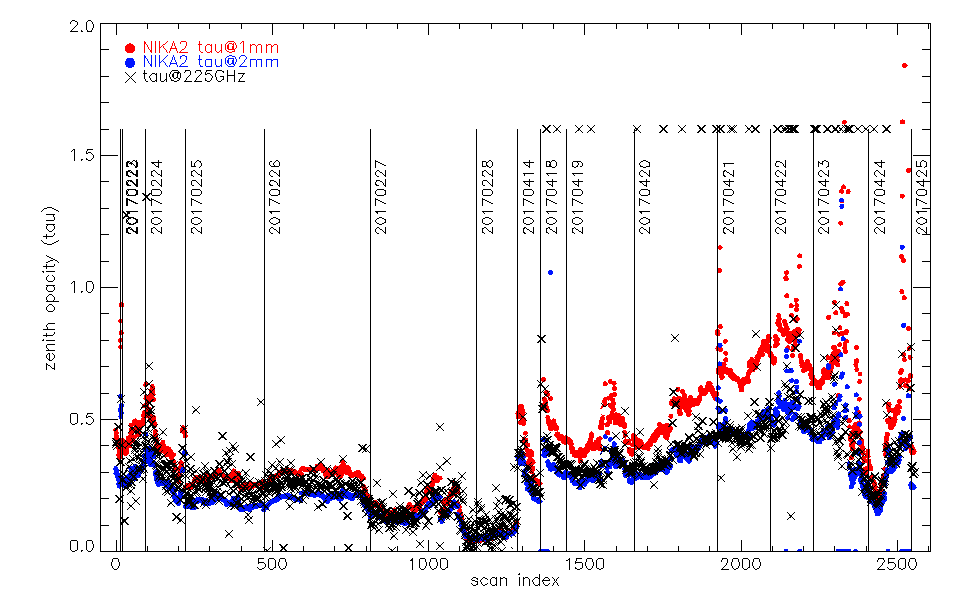
\includegraphics[width=\linewidth]{Figures/opacity_vs_index_N2R9_N2R10.png}
\caption{Atmospheric opacity as measured from the IRAM 225\,GHz
  taumeter (black crosses), and from the NIKA2 data at 150 (red) and 260\,GHz (blue) during 
  N2R9 and N2R10 commissioning campaigns.  We stress the fact that the IRAM 225\,GHz taumeter data is not used for the atmospheric correction and is plotted here just for comparison.
  \label{fig:taumeas}}
\end{center}
\end{figure}


In Fig.~\ref{fig:taumeas} {\bf(and Fig.~\ref{fig:taumeas_paper} of
  \ref{NIKA2-Tech}) } we present the evolution of the NIKA2 in-band
opacities for all the 'OTF' scans (about 1300 scans per runs) of the
N2R9 run held in February and the N2R10 run in April 2017. These are
compared to the IRAM tau-meter values. We observe an agreement on the global trend between the IRAM tau-meter opacity (225 GHz) and the NIKA2 values. These latter show, however,
a smaller dispersion (less than one percent).





\clearpage
%----------------------------------------------------------------------------------------
%	FOCAL PLANE RECONSTRUCTION
%----------------------------------------------------------------------------------------
\section{Focal Plane Reconstruction}
\label{se:fp_reconstruction}
%----------------------------------------------------------------------------------------
%	FOCAL PLANE RECONSTRUCTION
%----------------------------------------------------------------------------------------
%\subsection{Methodology}
\label{se:fov}

\begin{figure}[ht]
\begin{center}
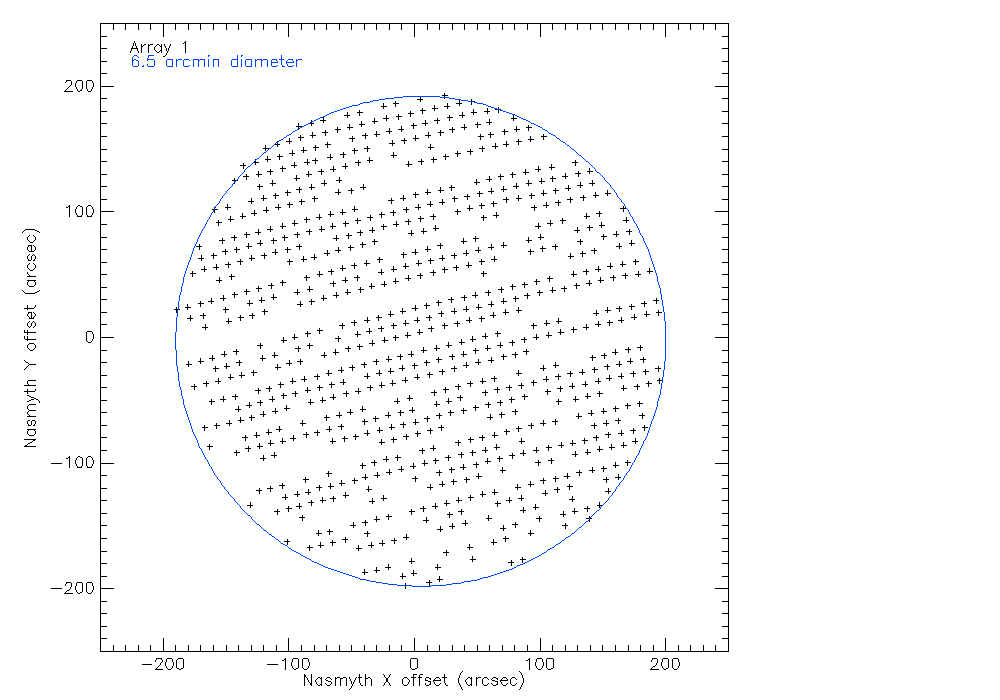
\includegraphics[clip, angle=0, scale = 0.15]{Figures/FOV_A1.png}
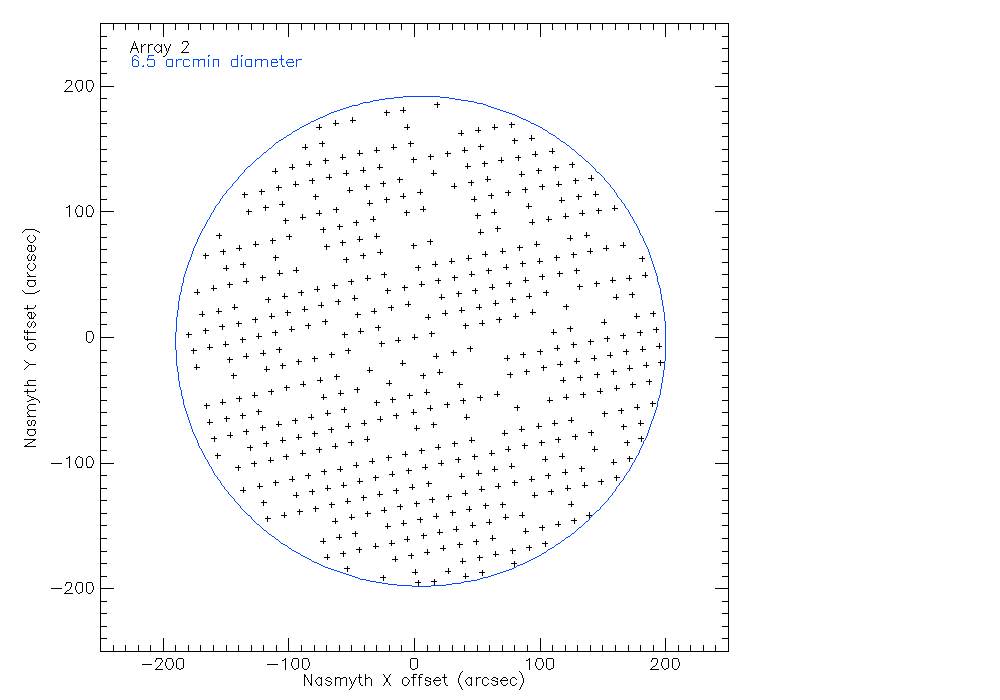
\includegraphics[clip, angle=0, scale = 0.15]{Figures/FOV_A2.png}
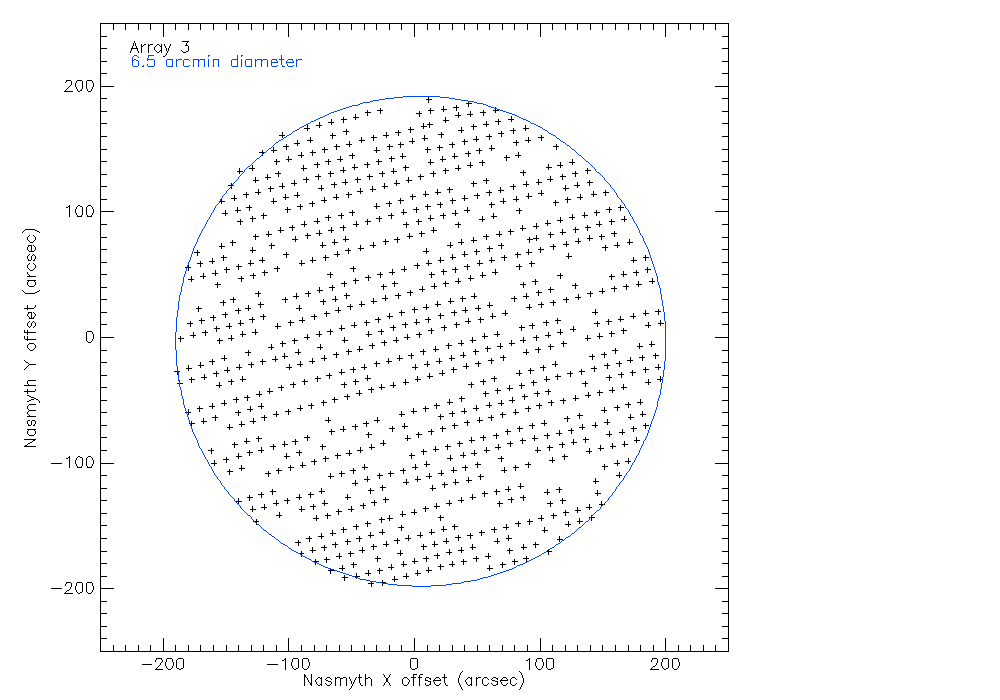
\includegraphics[clip, angle=0, scale = 0.15]{Figures/FOV_A3.png}
\caption{Nasmyth offsets of each array, from beammap 20170226s415 on
  3C84 (N2R9).}
\label{fig:fov_ex}
\end{center}
\end{figure}

% moved to the average FOV section
%\begin{table}
%\begin{tabular}{|l|l|l|}
%\hline
%Array & Number of valid kids & Fraction of all kids\\
%\hline
%A1 & 793 & 0.75\\
%A2 & 481 & 0.83\\
%A3 & 872 & 0.83\\
%\hline
%\end{tabular}
%\end{table}

In order to determine the pointing offsets of each KID w.r.t. the reference sky
coordinates as commanded by the telescope tracking system, we perform a
``beammap'', that is to say we map a bright and compact source, most of the time
a planet, with a elevation step small enough to meet Nyquist sampling at the 1mm
beam scale, namely 4.8~arcsec. We observe this planet with a raster scan in
(az,el) coordinates, either with fixed elevation subscans or fixed azimuth
subscans. The former has the advantage of low air mass variation across a
subscan, the latter offers an orthogonal scan direction to the former: the
combination of both gives a more accurage determination of the far side
lobes. The data reduction proceeds in two steps.

\paragraph{Step 1.} We apply a median filter per
KID timeline whose width is 4~FWHM and we project one map per KID in Nasmyth
coordinates. This median filter removes most of atmospheric and low frequency
electronic noise efficiently, albeit a slight ringing and flux loss on the
source. However, at this stage, we are only interested in the location of the
observed planet. To derive the Nasmyth coordinates from the provided (az,el)
coordinates, we build the following quantities at each time $t$

\begin{eqnarray}
dx_t &=& \cos el_t\, daz_t - \sin el_t\, del_t \nonumber \\
dy_t &=& \sin el_t\, daz_t + \cos el_t\, del_t \nonumber
\end{eqnarray}

where $el_t$ is the elevation of the reference pointing direction and $daz$ and
$del$ are the pointing offsets w.r.t to the source in azimuth and elevation as
provided by the tracking system. Note that $daz$ is already corrected by the
$\cos el_t$ factor to have orthonormal coordinates in the tangent plane of the sky
and be immune to the geodesic convergence at the poles. We then fit a 2D
elliptical gaussian on each kid map. The centroid of this gaussian is a first
estimate of the KID offsets, FWHM's, ellipticity and sensitivity. We apply a
first KID selection by removing outliers to the statistics on these
parameters. We also discard manually KIDs that show a cross-talk counter part on
their map. At the end of this first step, we are ready to move to a second
stage.

\paragraph{Step 2.} With the Nasmyth offsets derived in step 1, we are now able to
mask out the planet in each KID timeline. This mask is centered on the planet
location as seen by each kid, it is circular and has a radius of 60~arcsec. We
now build a template timeline (a.k.a. ``common mode'') in two steps. First, we
take the median of all samples of all KIDs that are outside this mask at a given
time $t$. This gives a first estimate of the common mode. Second, we
cross-calibrate each KID on this common mode when the KID is outside the mask
and we coadd all these KID cross-calibrated timelines when they are outside the
mask to have the final common mode. In this sum, each KID TOI is weighted by the
inverse of its variance outside the mask. Once we have this common mode in hand,
we cross-calibrate each TOI on it outside the mask and we subtract it to the
entire KID TOI. When then resume to the projection of each KID TOI in Nasmyth
coordinates like in step 1, and the 2D elliptical gaussian fit on the each kid
map. The centroid coordinates and the FWHM are now the final parameters that can
be derived on the current scan.

This analysis is repeated on all the beam maps, which provides statistics and
precision on each KID parameter, together with estimates on KID performance stability.

{\bf show a screen capture of Katana.}\\

% LP: j'ajoute une phrase pour referencer la Figure \ref{fig:fov}
We present an example of the FOV reconstruction in Fig.~\ref{fig:fov_ex}.

\begin{equation}
FOV diameter = \sqrt{4 N_{tot. kids} * gridstep^2/\pi}
\end{equation}

{\bf give the values of gridstep (pitch) both in mm and arcsec on the sky}\\

The same definition applies to ``Effective FOV'' to avoid extra multiplication
by the fraction of valid pixels

\begin{equation}
F\lambda = gridstep\times D(30m)/\lambda
\end{equation}

%\subsection{Average Focal Plane Reconstruction}
\label{avg_kidpar}

\begin{figure}
\begin{center}
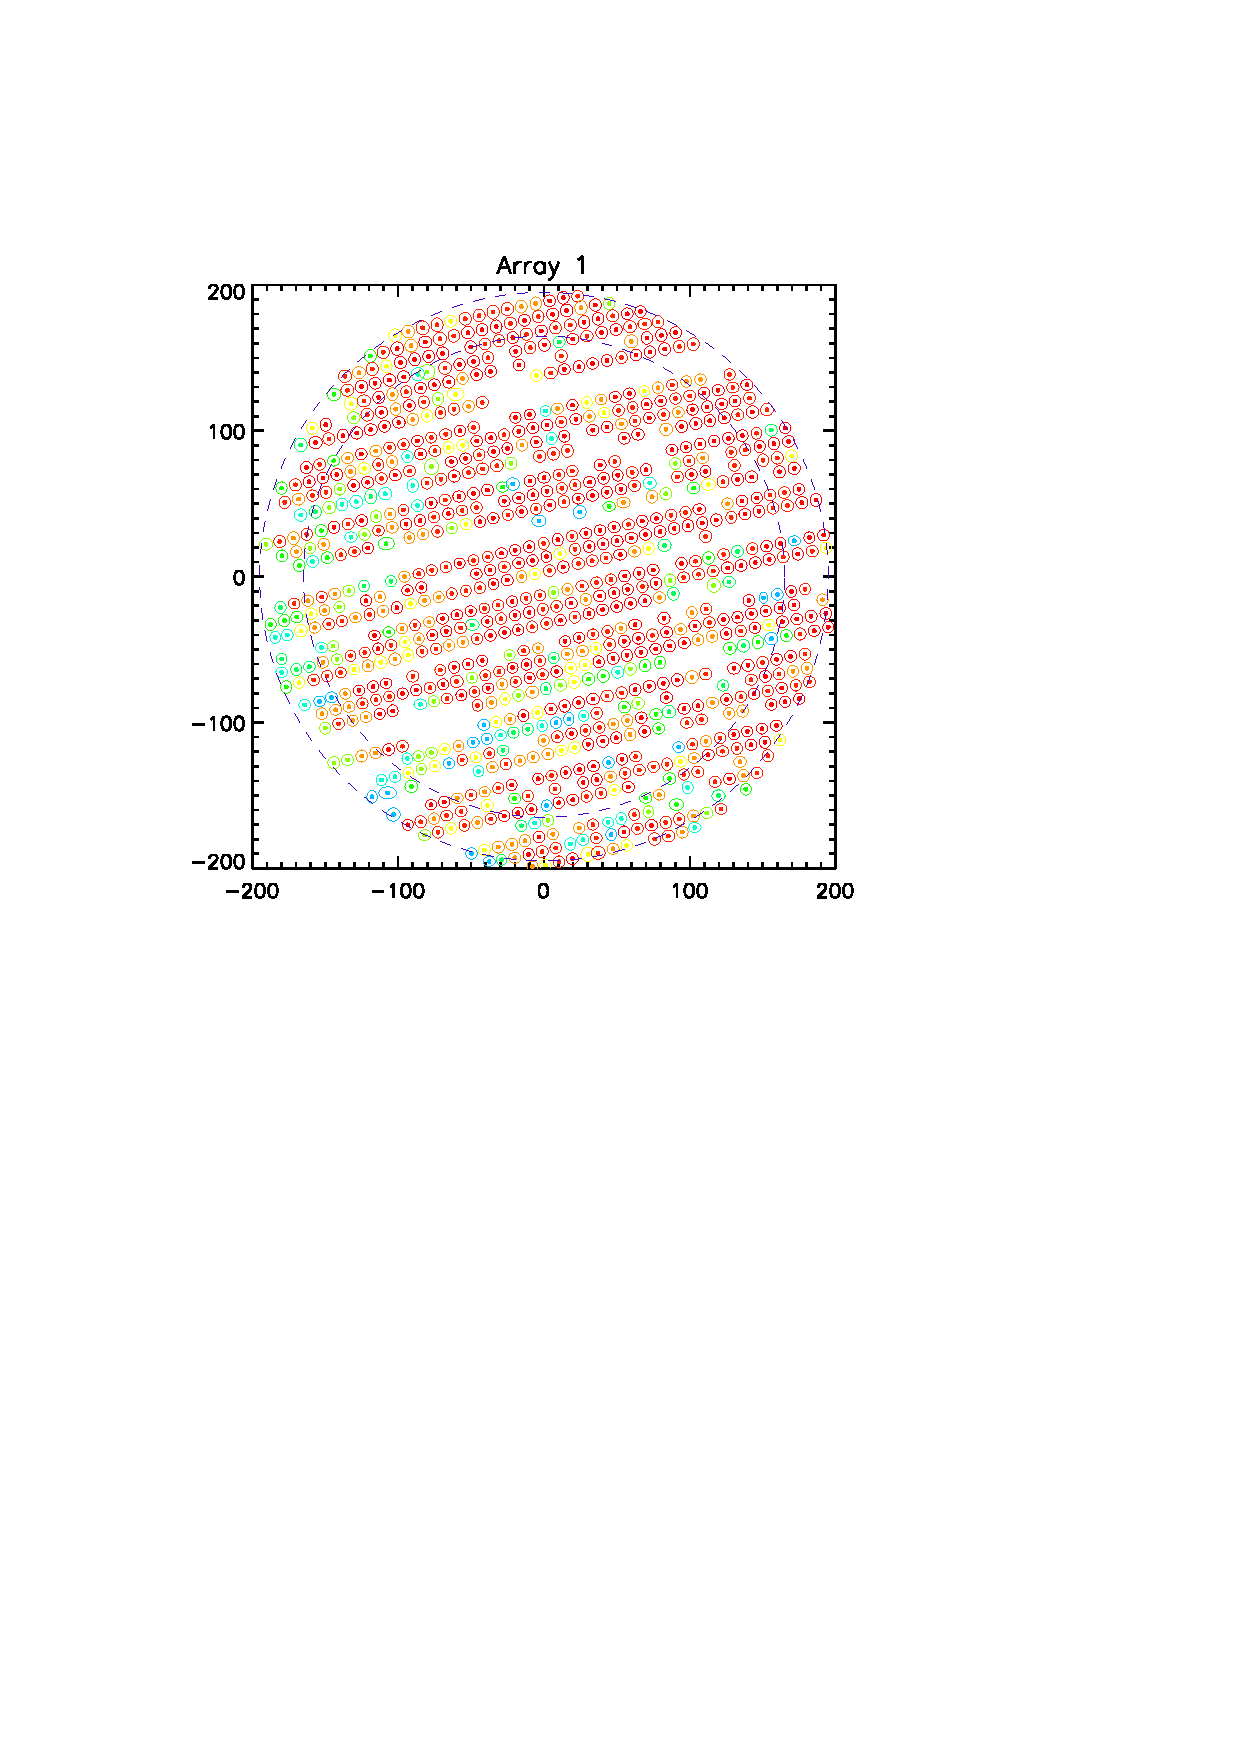
\includegraphics[trim=2cm 14cm 5cm 4cm, clip=true,width=0.6\linewidth]{Figures/A1_fwhm_color_count.pdf}
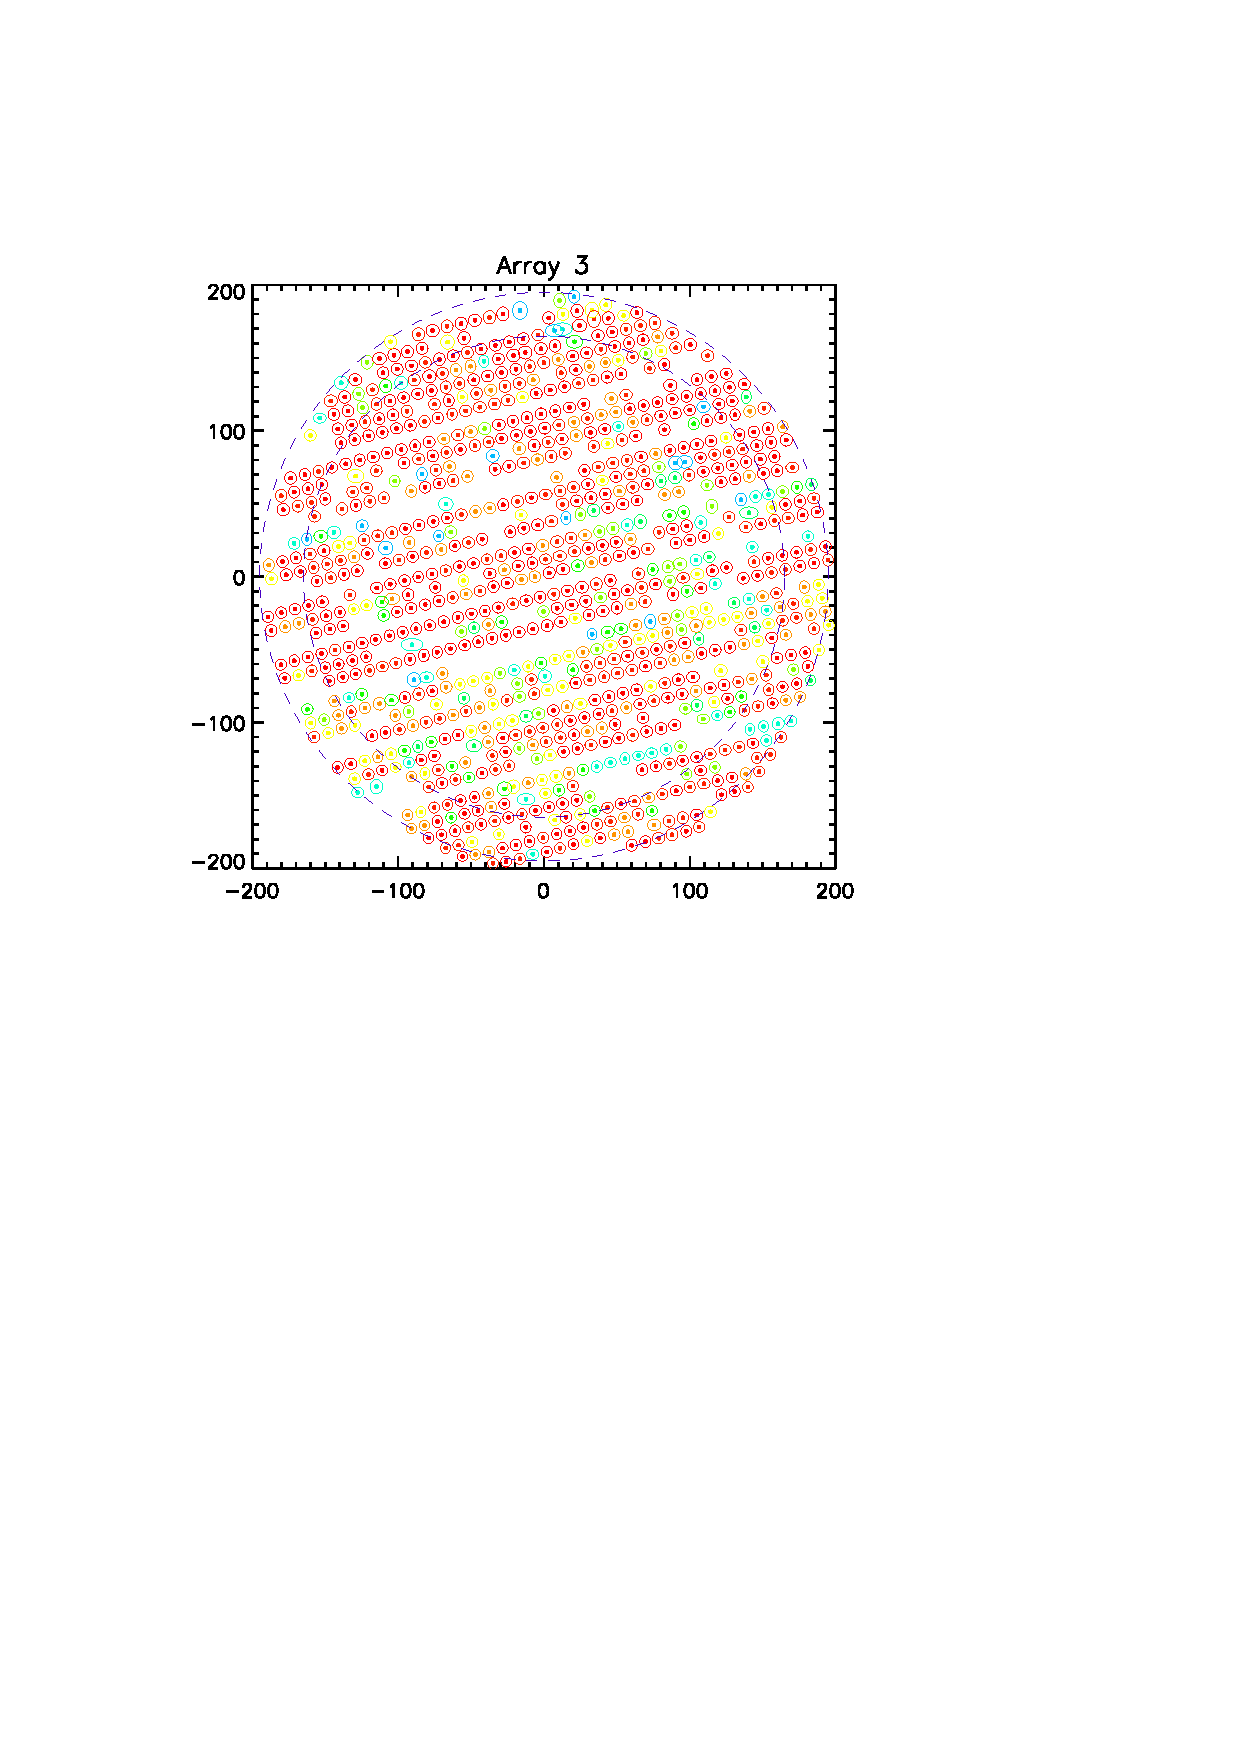
\includegraphics[trim=2cm 14cm 5cm 4cm, clip=true,width=0.6\linewidth]{Figures/A3_fwhm_color_count.pdf}
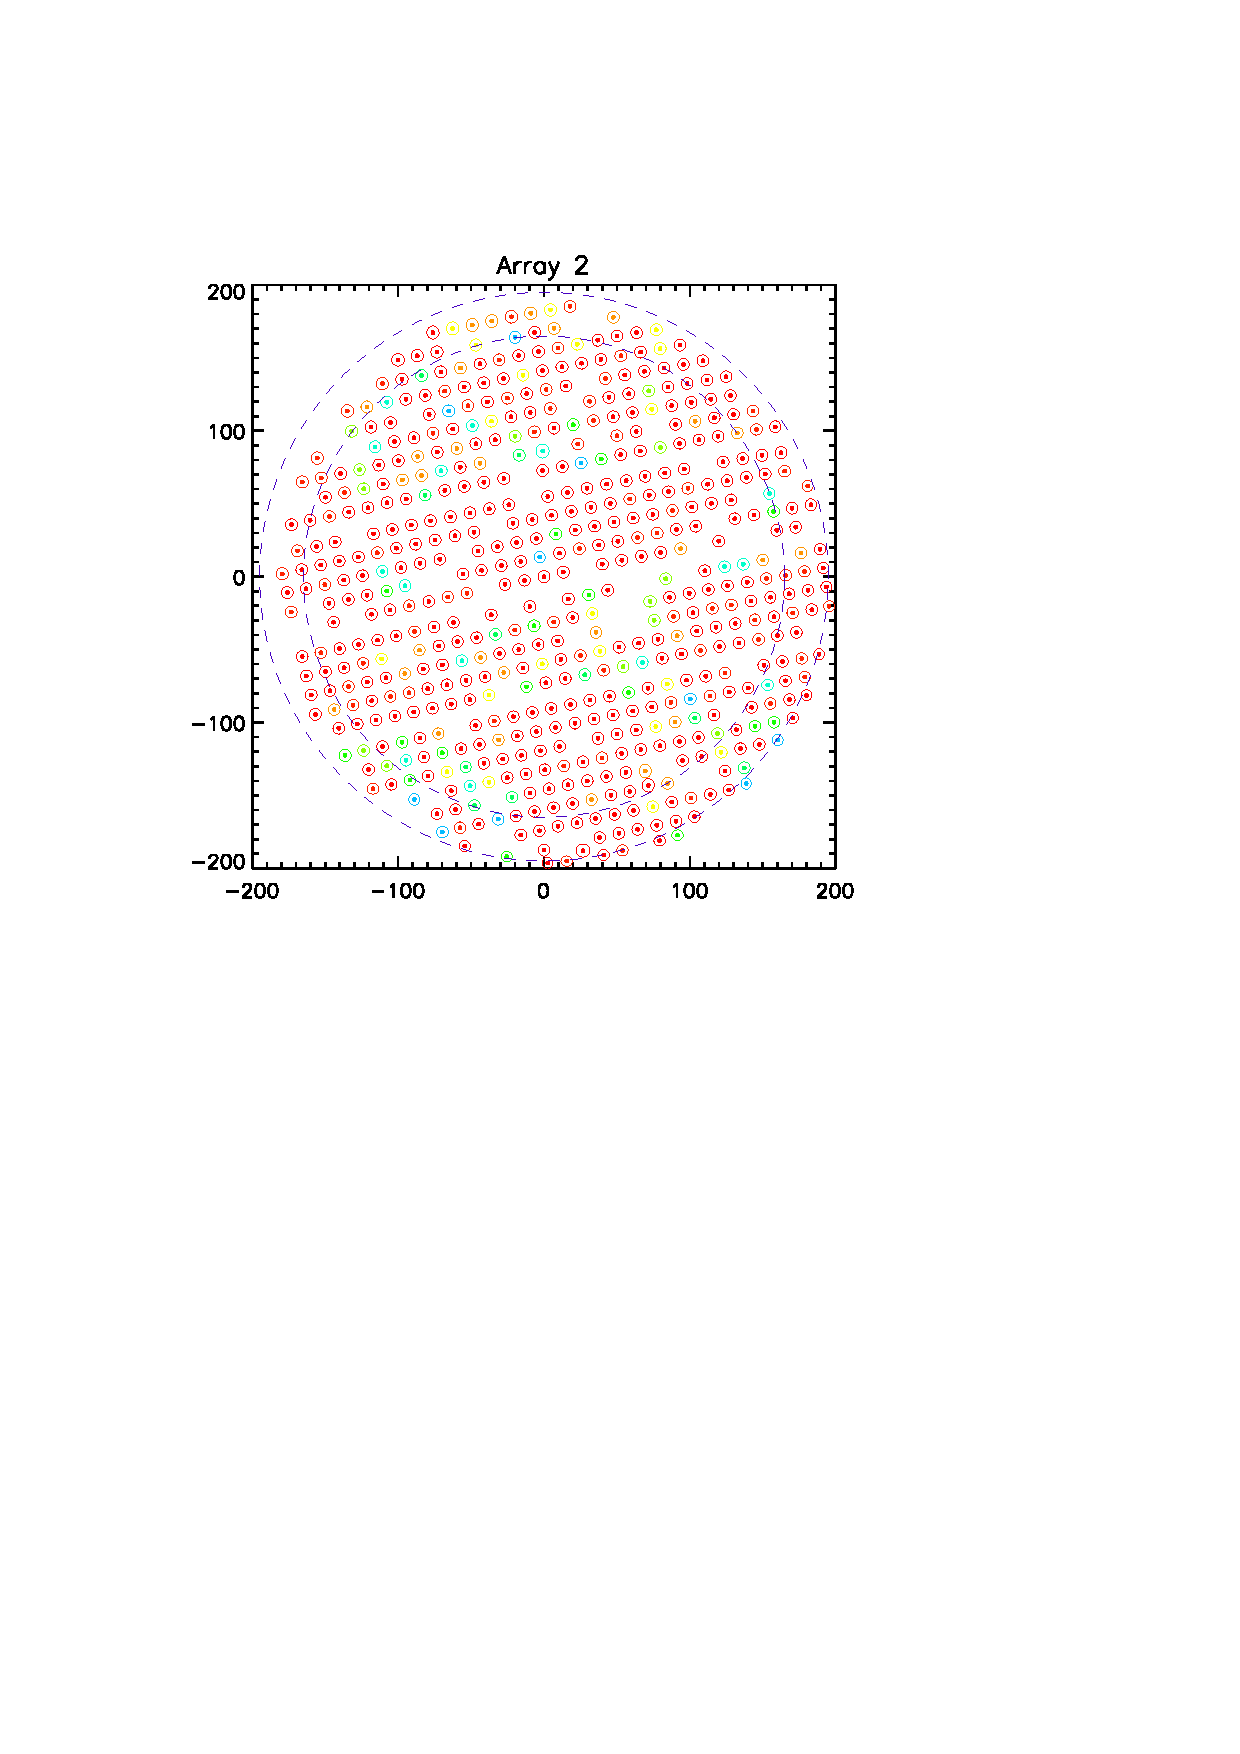
\includegraphics[trim=2cm 14cm 5cm 4cm, clip=true,width=0.6\linewidth]{Figures/A2_fwhm_color_count.pdf}
\caption{Average detectors positions for arrays A1, A3, and A2 (from
  green to red as a function of the number of times that a given pixel
  has been considered as valid). The three plots show the detectors
  that have seen the sky and passed the quality criteria for at least
  two beam maps during Run10, 9 and 8: 952, 961, and 553
  %925, 944, and 543
  for A1, A3 and A2, respectively. The inner and outer dash-line circles correspond to a FOV of 5.5$\prime$ and 6.5$\prime$, respectively. Units are arcseconds. The color (from green to red)  shows the number of times that a given pixel has been considered as valid.}
\label{fig:avg_fov_color}
\end{center}
\end{figure}

In order to identify the most stable pixels, we compare the KIDs parameter obtained with several beam maps. 
In the following we will show results as obtained using seven beam maps from Run10, two from Run9 and one from Run8.
For each pixel we compute the average position on the focal plane and the average FWHM, counting the times that it has been considered as valid.

In Fig. \ref{fig:avg_fov_color} we show the average focal plane
reconstruction, from green to red depending on the number of times
that the pixel has been considered as valid. For A1, A3 and A2,
respectively, we have 952, 961, and 553 pixels that have been
considered as valid at least twice (840, 508, 868 valid at least five
times).
% LP: add a sentence to reference Table ``\ref{tab:number_of_kids}"
Using this criterion, we deduce the fraction of valid
detectors over the designed ones, as given in Table~\ref{tab:number_of_kids}. 
As a second step, we also flag pixels that move across the focal plane from a beam map to another (Fig. \ref{fig:jumping_kids} , jumping KIDs) and those who share the same position (twin KIDs). To identify the former we look at the difference of the mean and median position of each KID (the red crosses and black squares in Fig. \ref{fig:mean_vs_median}). For the latter a criteria on the position is applied in order to find the pixels that are closer than the grid step.

\begin{figure}
\begin{center}
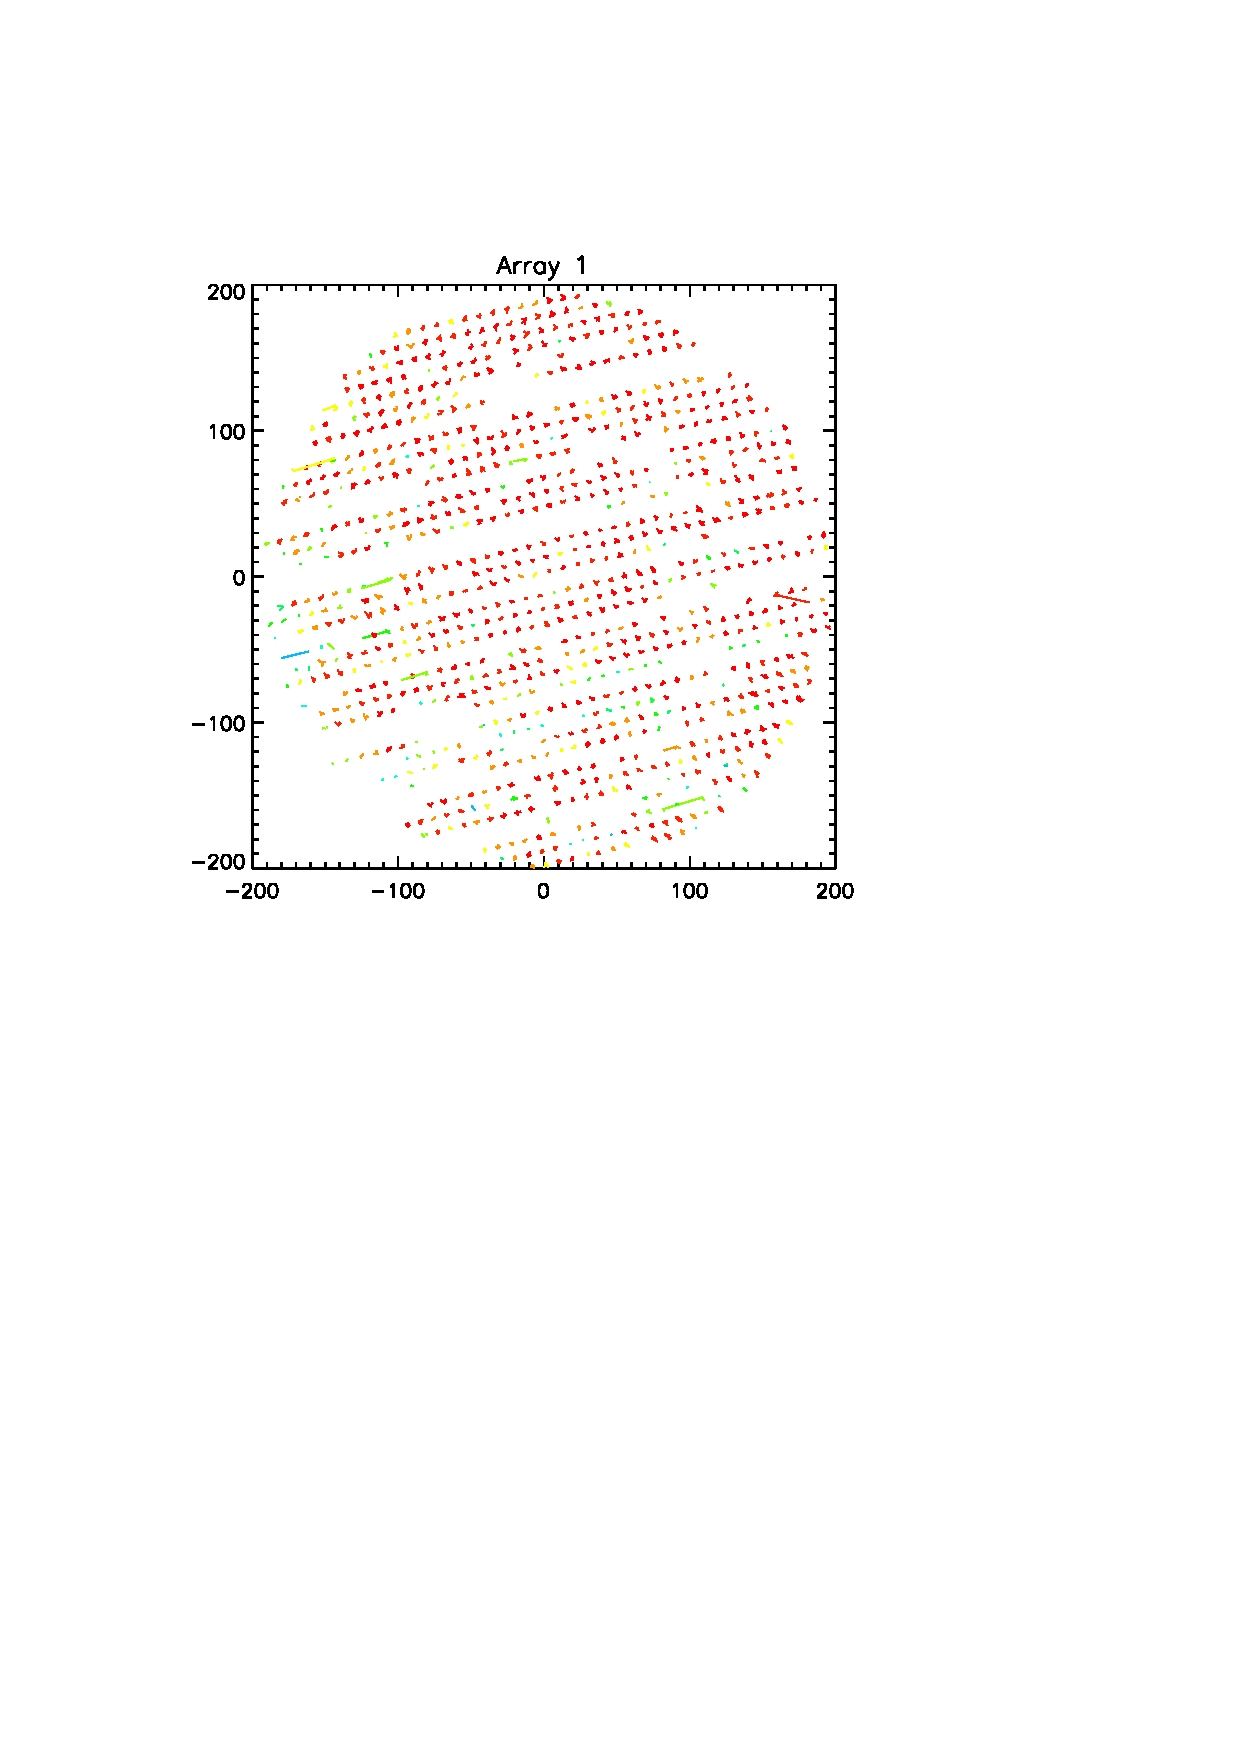
\includegraphics[trim=2cm 14cm 5cm 4cm, clip=true,width=0.6\linewidth]{Figures/A1_positions.pdf}
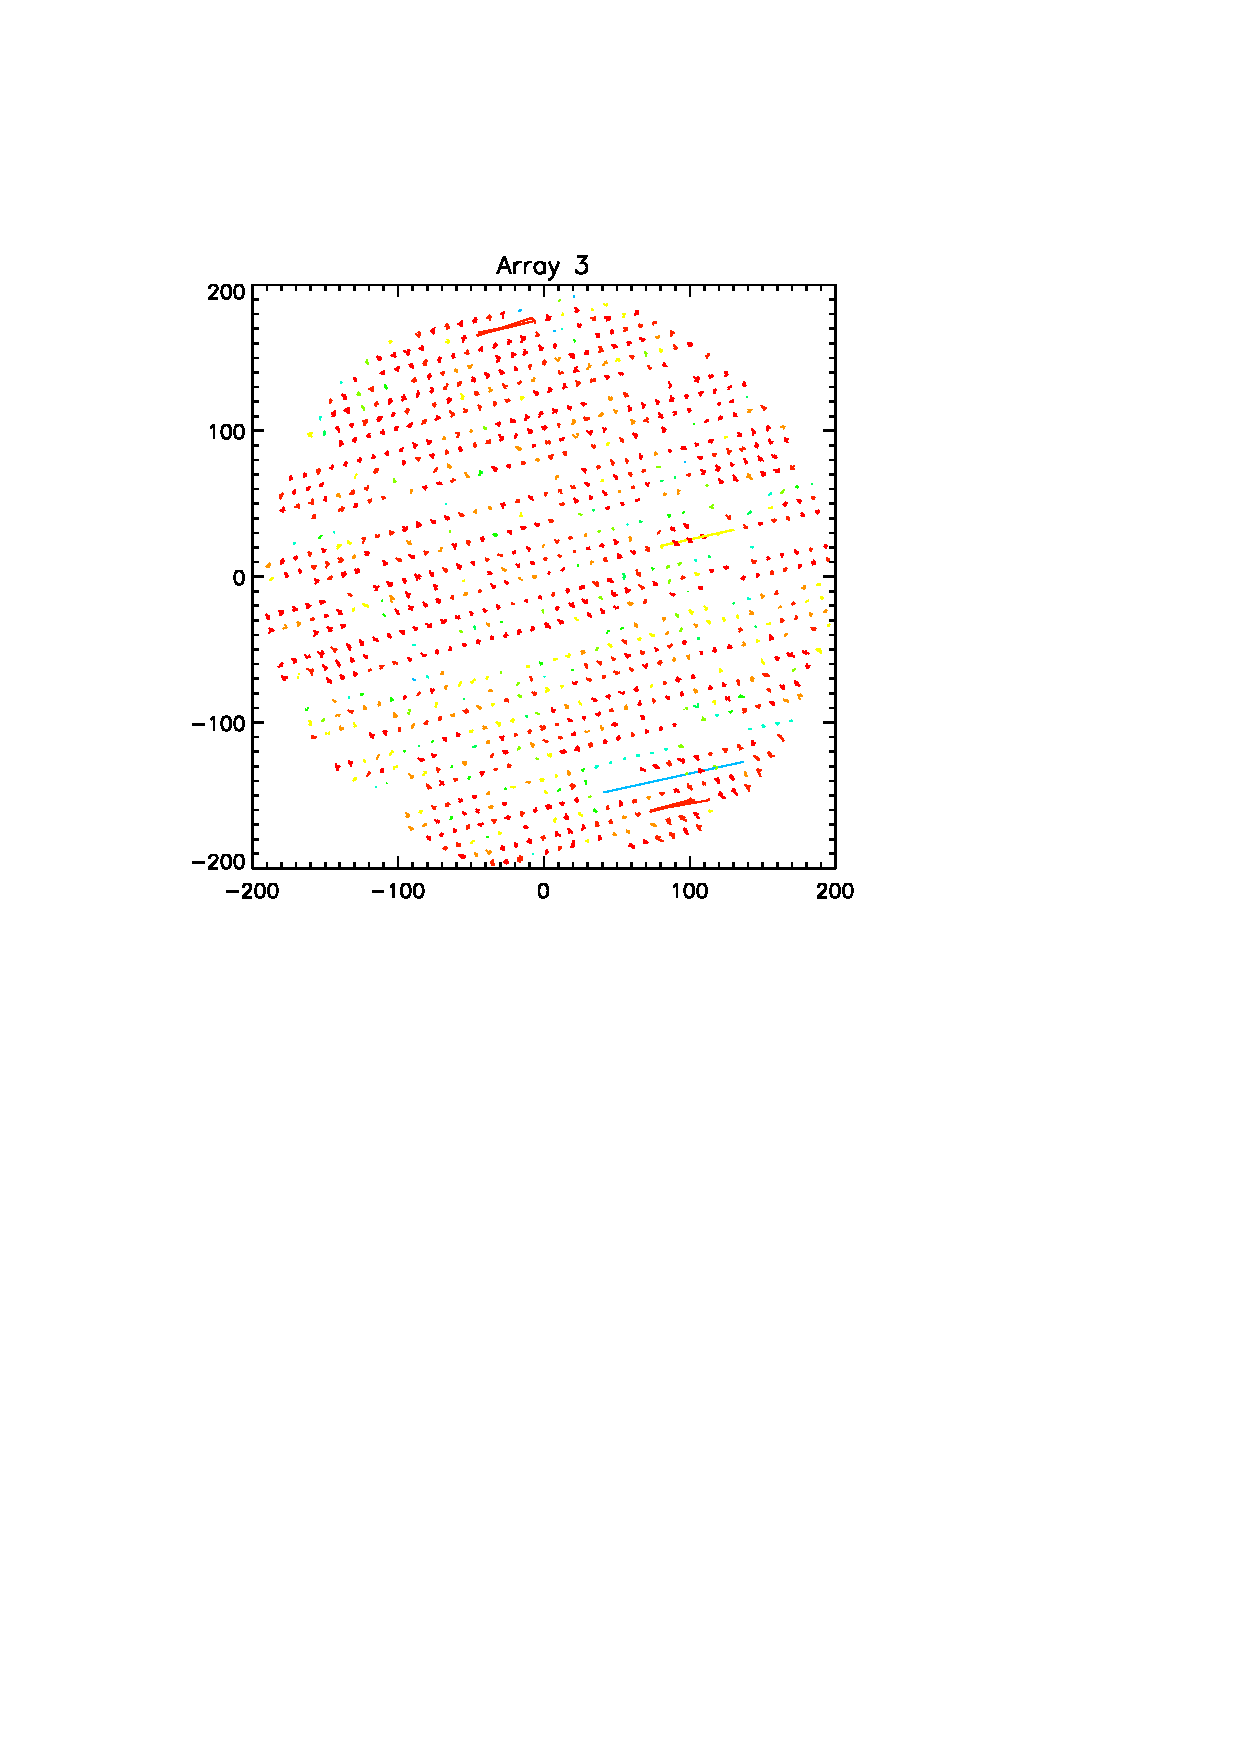
\includegraphics[trim=2cm 14cm 5cm 4cm, clip=true,width=0.6\linewidth]{Figures/A3_positions.pdf}
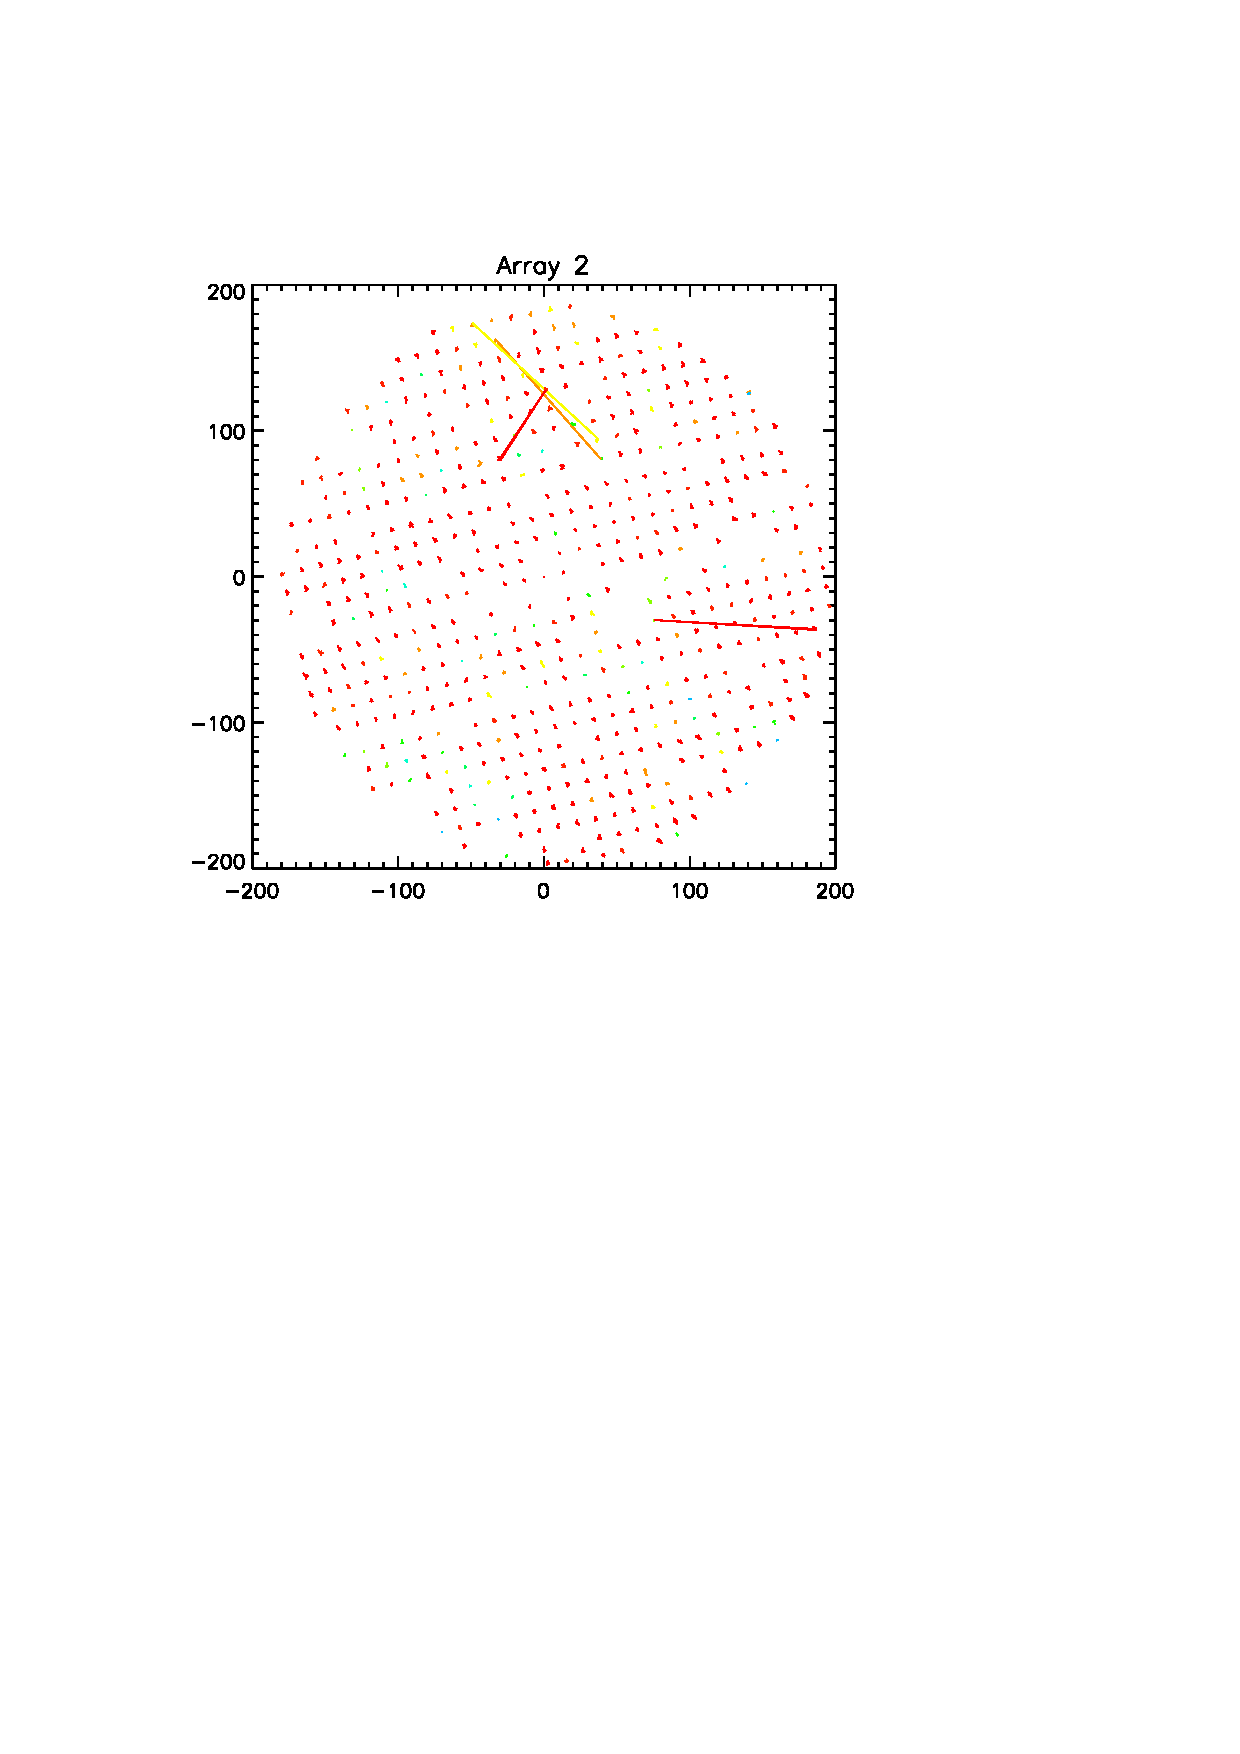
\includegraphics[trim=2cm 14cm 5cm 4cm, clip=true,width=0.6\linewidth]{Figures/A2_positions.pdf}
\caption{For the 952, 961, and 553 pixels that have passed the quality criteria at least twice for A1, A3 and A2, we show the positions of each pixel, as obtained from each beam map. We can see that some of them are not found at the same position for all the beam maps. Units are arcseconds.}
\label{fig:jumping_kids}
\end{center}
\end{figure}

\begin{figure}
\begin{center}
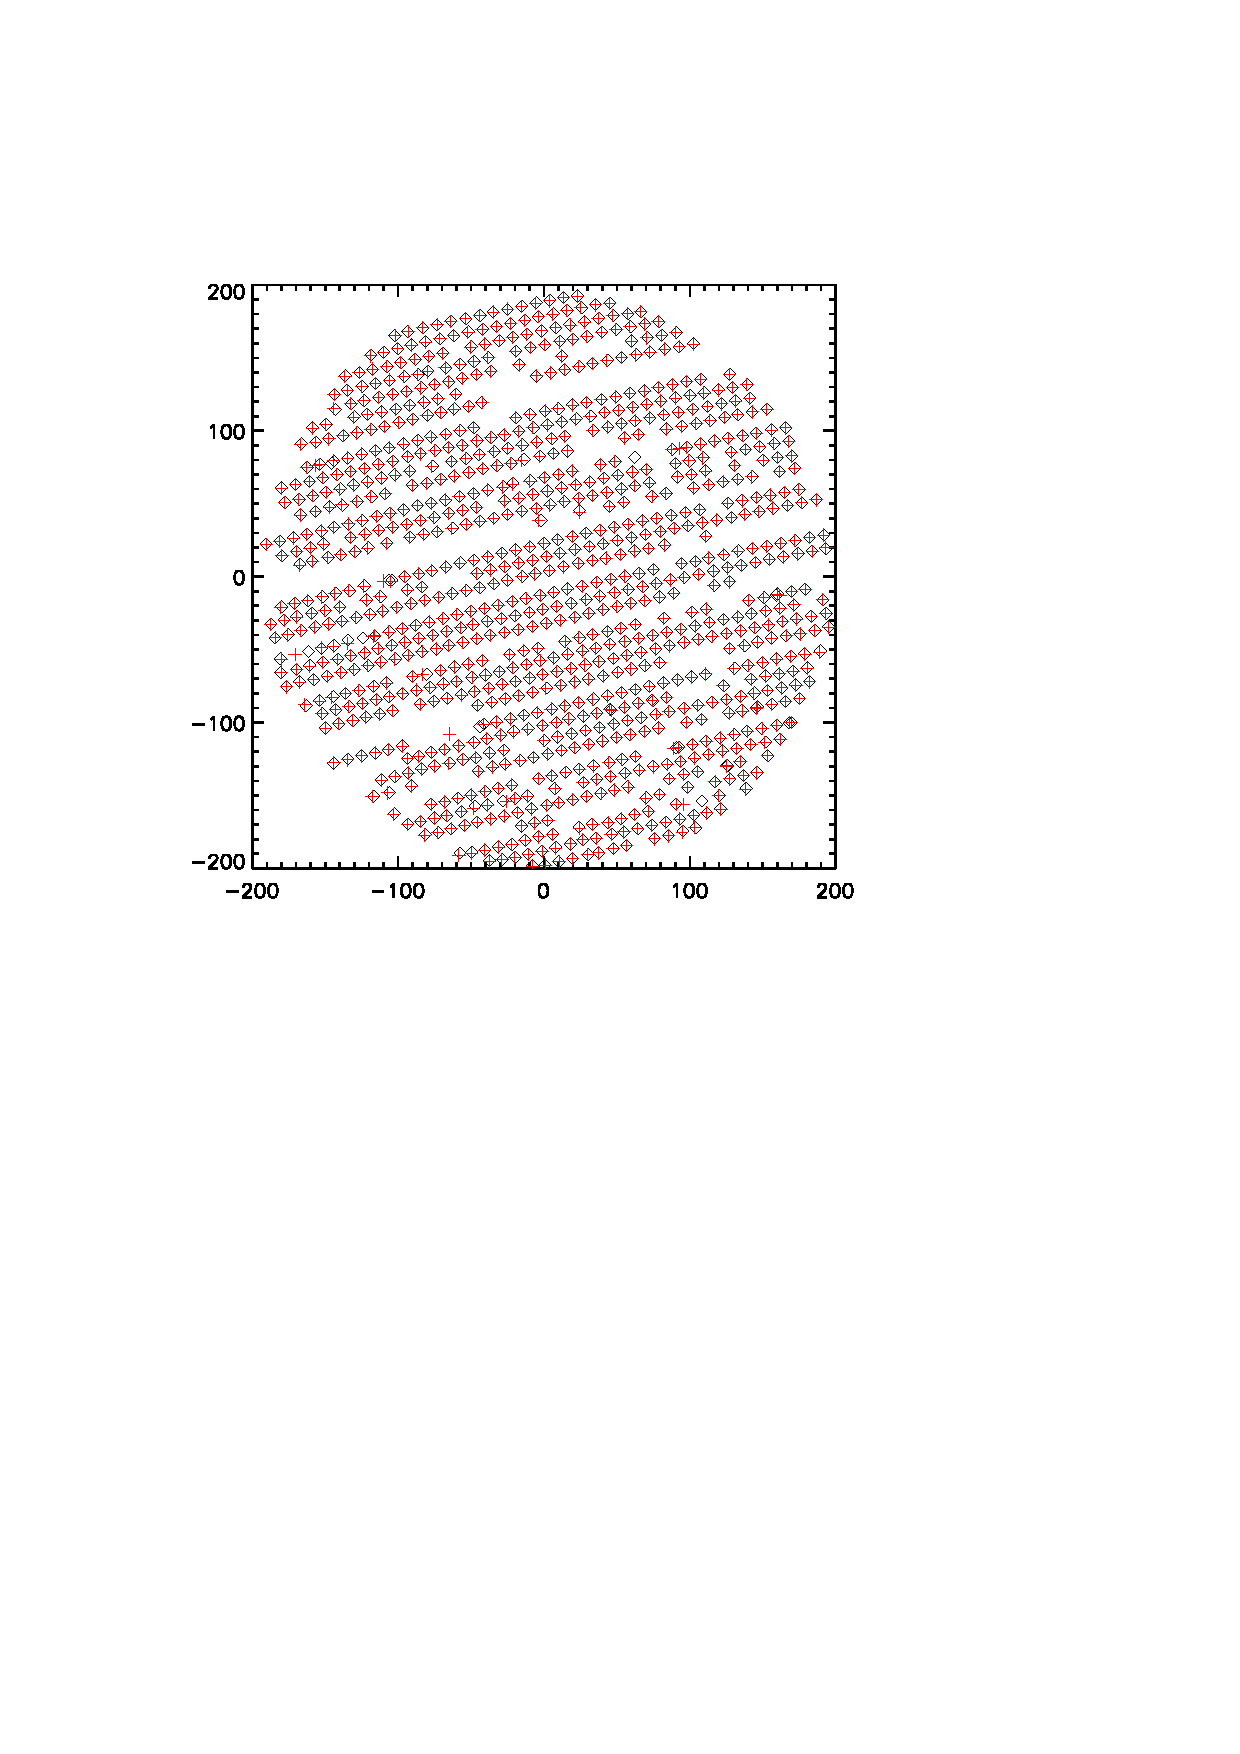
\includegraphics[trim=2cm 14cm 5cm 4cm, clip=true,width=0.6\linewidth]{Figures/A1_test_positions.pdf}
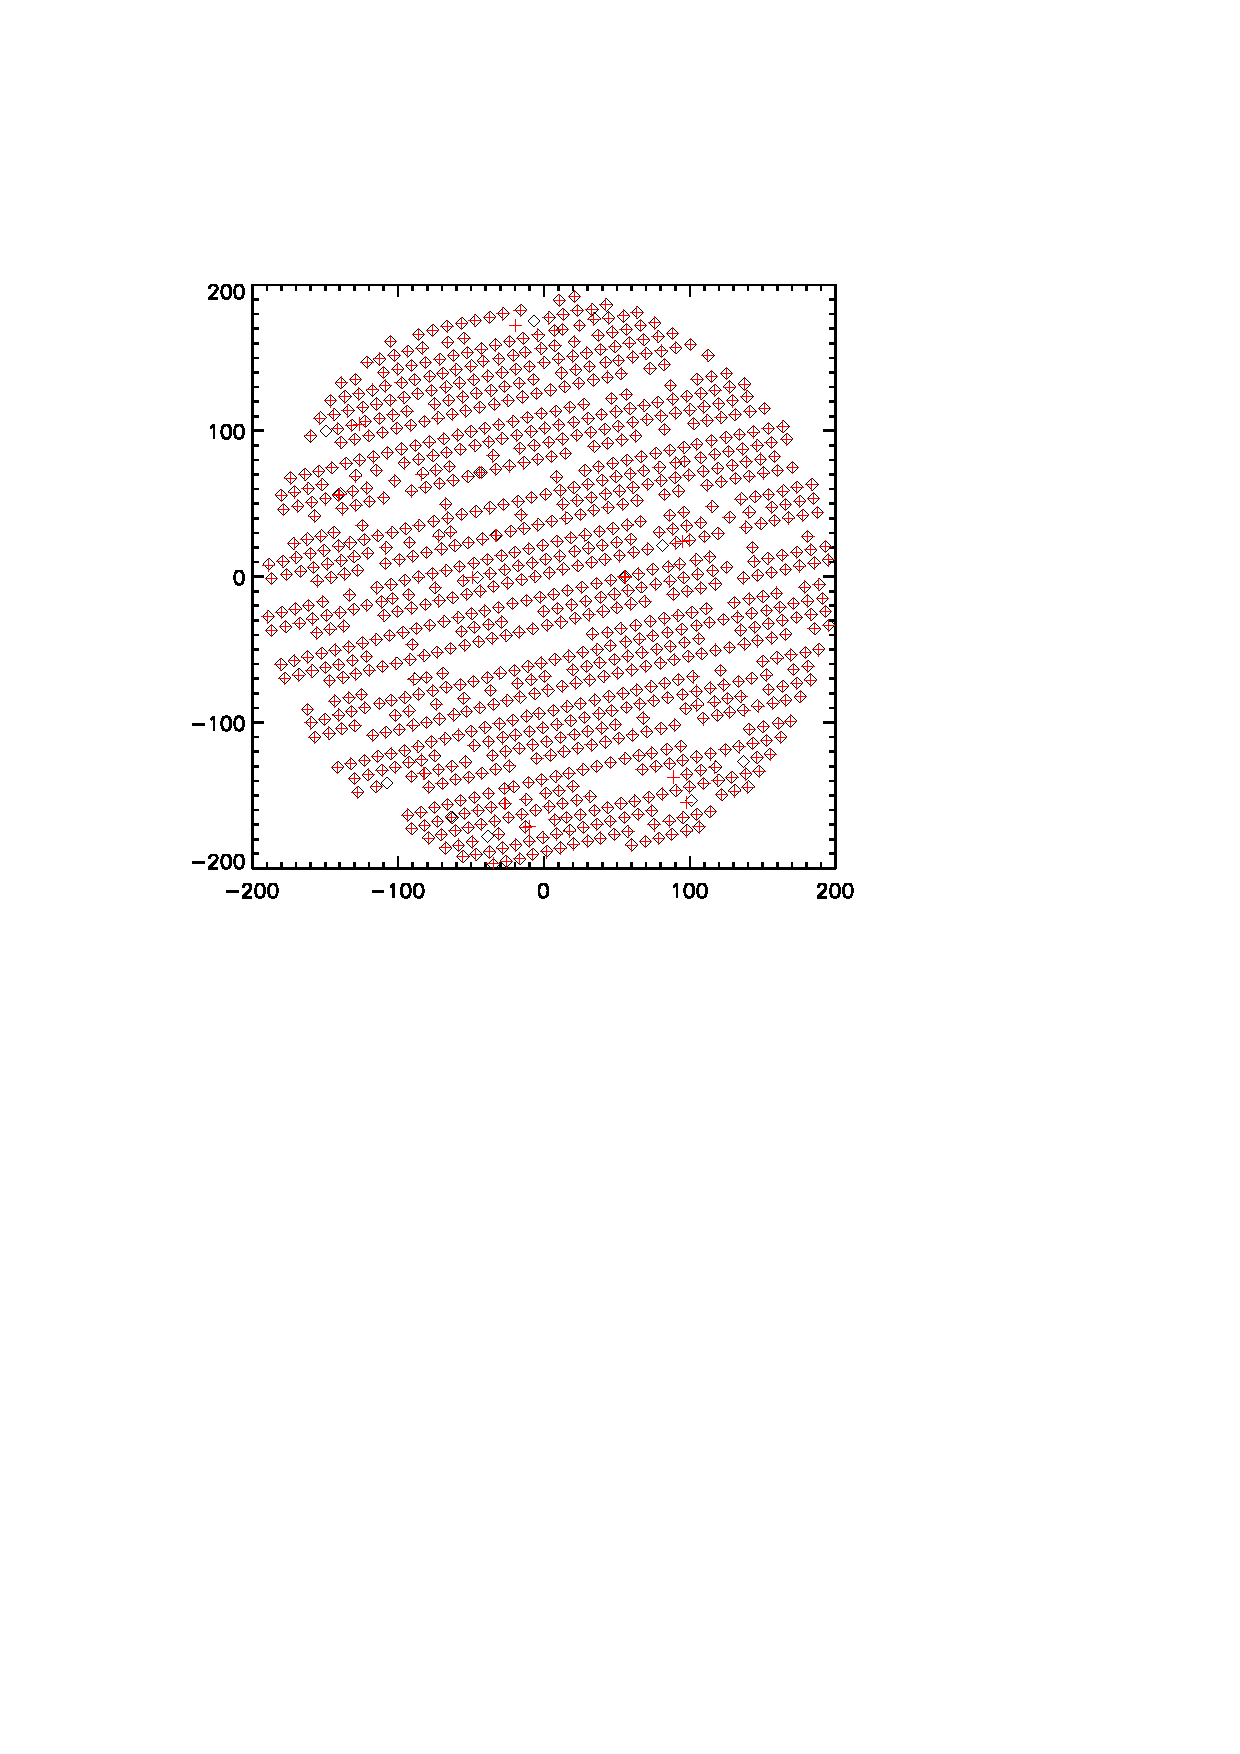
\includegraphics[trim=2cm 14cm 5cm 4cm, clip=true,width=0.6\linewidth]{Figures/A3_test_positions.pdf}
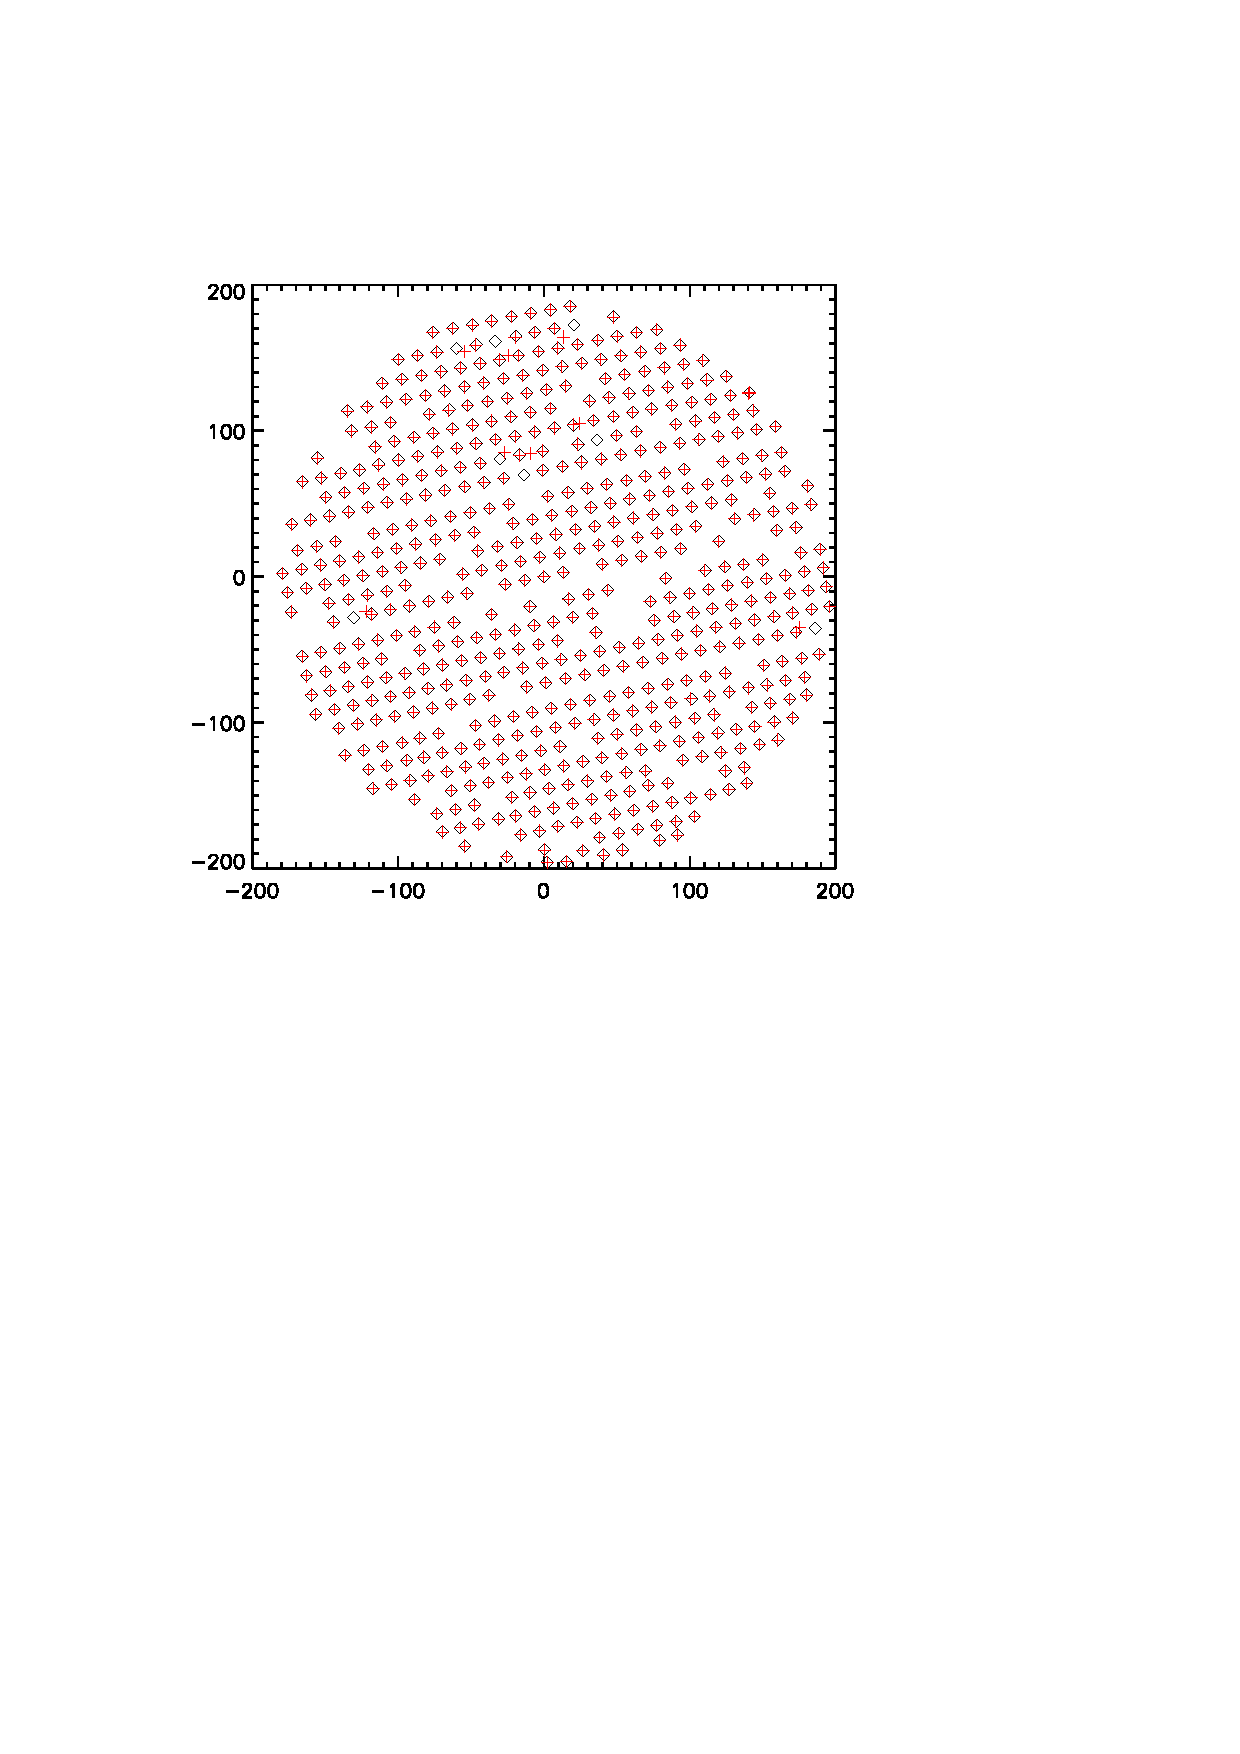
\includegraphics[trim=2cm 14cm 5cm 4cm, clip=true,width=0.6\linewidth]{Figures/A2_test_positions.pdf}
\caption{For the 952, 961, and 553 pixels that
  have passed the quality criteria at least twice for A1, A3 and A2,
  we show the mean (red crosses) and the median (black squares)
  positions of each pixel, as obtained from each beam map.
  Units are arcseconds. }
\label{fig:mean_vs_median}
\end{center}
\end{figure}


% LP: copy from fov.tex + modif according to Samuel's comment
\begin{table}
  \label{tab:number_of_kids}
  \begin{tabular}{|r|r|r|r|}
    \hline
    Array & Number of designed detectors &  Number of valid detectors & Fraction of all detectors\\
    \hline
    A1 & 1140 & 952 &  0.84\\
    A3 & 1140 & 961 &  0.84\\
    A2 & 616  & 553 &  0.90\\
    \hline
  \end{tabular}
\end{table}

%\subsection{FOV grid distortion}
\label{se:grid_distortion}

{\bf LP edit using Samuel's comments, [TBC]}

We studied the matching of the KIDs position on the sky to the
\emph{design} position, as decribed in Xavier's wiki post\footnote{see
  {\tt http$://$www.iram.fr$/$wiki$/$nika2$/$index.php$/$}
  
  {\tt April$\_$19,$\_$2017,$\_$FXD,$\_$KID$\_$position$\_$mapping$\_$and$\_$Field$\_$distortion$\_$for$\_$Run9}
}

This has been compared to expectations obtained using ZEMAX
simulation. The grid diagram generated using ZEMAX provides us with
the maximum dispersion in the field defined by

\begin{equation}
P = \frac{\sqrt{(x_p - x_r)^2 + (y_p - y_r)^2}}{\sqrt{x_p^2 + y_p^2}},
\end{equation}

where $(x_p, y_p)$ and $(x_r, y_r)$ are respectivelly the predicted
and real coordinates on the image surface relative to the reference
field position image location (see page 170 of the ZEMAX manual, 2007).
The predicted coordinates for the whole field are obtained using a
linear interpolation of a small area in the field central part,
whereas the real coordinates are calculated by ray tracing through the
optical system.

\begin{figure}[ht] 
\begin{center}
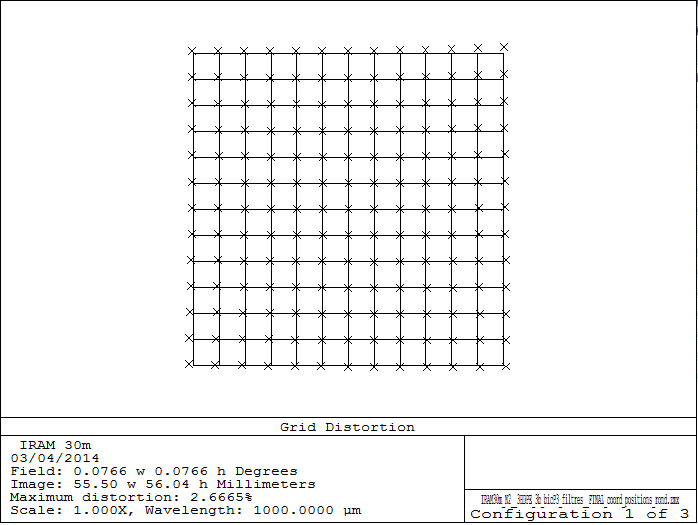
\includegraphics[width=0.9\textwidth]{Figures/NIKA2_Final_grid.png}
\caption{NIKA2 grid diagram simulated using ZEMAX. Crosses indicate
  the real coordinates on the Nasmyth image plan. {\bf question a
    Samuel: pourquoi les dimensions indiquees sont environs 4.5 arcmin
  de cote (et pas 6.5)?}}
 \label{fig:fov_grid_distortion_zemax}
\end{center}
\end{figure}

Figure \ref{fig:fov_grid_distortion_zemax} show the ZEMAX grid diagram for
NIKA2 simulated optic system. The maximum grid distortion is expected
to be of $2.7\%$ in NIKA2 $6.5'$ FOV. The distortion is the most
noticeable in the upper right corner of the Nasmyth plan, which is
also the area of the largest defocus w.r.t. to the center. 




%   Geometry
%----------------------------------------------------------------------------------------
\subsection{Focal Plane Geometry}

In order to determine the pointing offsets of each KID with respect to the reference sky
coordinates as commanded by the telescope tracking system, we use beam-maps. 
The data reduction proceeds in two steps.

\paragraph{Step 1.} We apply a median filter per
KID timeline whose width is 4~FWHM and we project one map per KID in Nasmyth
coordinates. This median filter removes efficiently most of the atmospheric and low frequency
electronic noise, albeit a slight ringing and flux loss on the
source. However, at this stage, we are only interested in the location of the
observed planet. To derive the Nasmyth coordinates from the provided (az,el)
coordinates, we build the following quantities at time~$t$ :

\begin{eqnarray}
dx_t &=& \cos el_t\, daz_t - \sin el_t\, del_t \nonumber \\
dy_t &=& \sin el_t\, daz_t + \cos el_t\, del_t \nonumber
\end{eqnarray}

\noindent {\bf FM: why not using $\delta$ as in the previous section ?}\\
\noindent {\bf FM: i don't think the $_t$ is useful}\\


where $el_t$ is the elevation of the reference pointing direction and $daz$ and
$del$ are the pointing offsets with respect to the source in azimuth and elevation as
provided by the tracking system. Note that $daz$ is already corrected by the
$\cos el_t$ factor to have orthonormal coordinates in the tangent plane of the sky
and be immune to the geodesic convergence at the poles. We then fit a 2D
elliptical gaussian on each kid map. The centroid of this gaussian is a first
estimate of the KID offsets, FWHM's, ellipticity and sensitivity. We apply a
first KID selection by removing outliers to the statistics on these
parameters. We also discard manually KIDs that show a cross-talk counter part on
their map. 
%At the end of this first step, we are ready to move to a second stage.

\paragraph{Step 2.} With the Nasmyth offsets derived in step 1, we are now able to
mask out the planet in each KID timeline. This mask is centered on the planet
location as seen by each kid, it is circular and has a radius of 60~arcsec. We
now build a template timeline (a.k.a. ``common mode'') in two steps. First, we
take the median of all samples of all KIDs that are outside this mask at a given
time $t$. This gives a first estimate of the common mode. Second, we
cross-calibrate each KID on this common mode when the KID is outside the mask
and we coadd all these KID cross-calibrated timelines when they are outside the
mask to have the final common mode. In this sum, each KID TOI is weighted by the
inverse of its variance outside the mask. Once we have this common mode in hand,
we cross-calibrate each TOI on it outside the mask and we subtract it to the
entire KID TOI. We then resume to the projection of each KID TOI in Nasmyth
coordinates like in step 1, and the 2D elliptical gaussian fit on the each kid
map. The centroid coordinates and the FWHM are now the final parameters that can
be derived on the current scan.

This analysis is repeated on all beam maps, which provides statistics and
precision on each KID parameter, together with estimates on KID performance stability.



{\bf FM : {\it precision} ? }\\
{\bf show a screen capture of Katana.}\\

% LP: j'ajoute une phrase pour referencer la Figure \ref{fig:fov}
We present an example of the FOV reconstruction in Fig.~\ref{fig:fov_ex}.

The FOV diameter is defined as 
\begin{equation}
FOV diameter = \sqrt{4 N_{tot. kids} \times gridstep^2/\pi}
\end{equation}

{\bf give the values of gridstep (pitch) both in mm and arcsec on the sky}\\

The same definition applies to ``Effective FOV'' to avoid extra multiplication
by the fraction of valid pixels

\begin{equation}
F\lambda = gridstep\times D(30m)/\lambda
\end{equation}




%   KID selection
%----------------------------------------------------------------------------------------
\subsection{KID selection and average geometry}
\label{avg_kidpar}


\begin{figure}[p]
\begin{center}
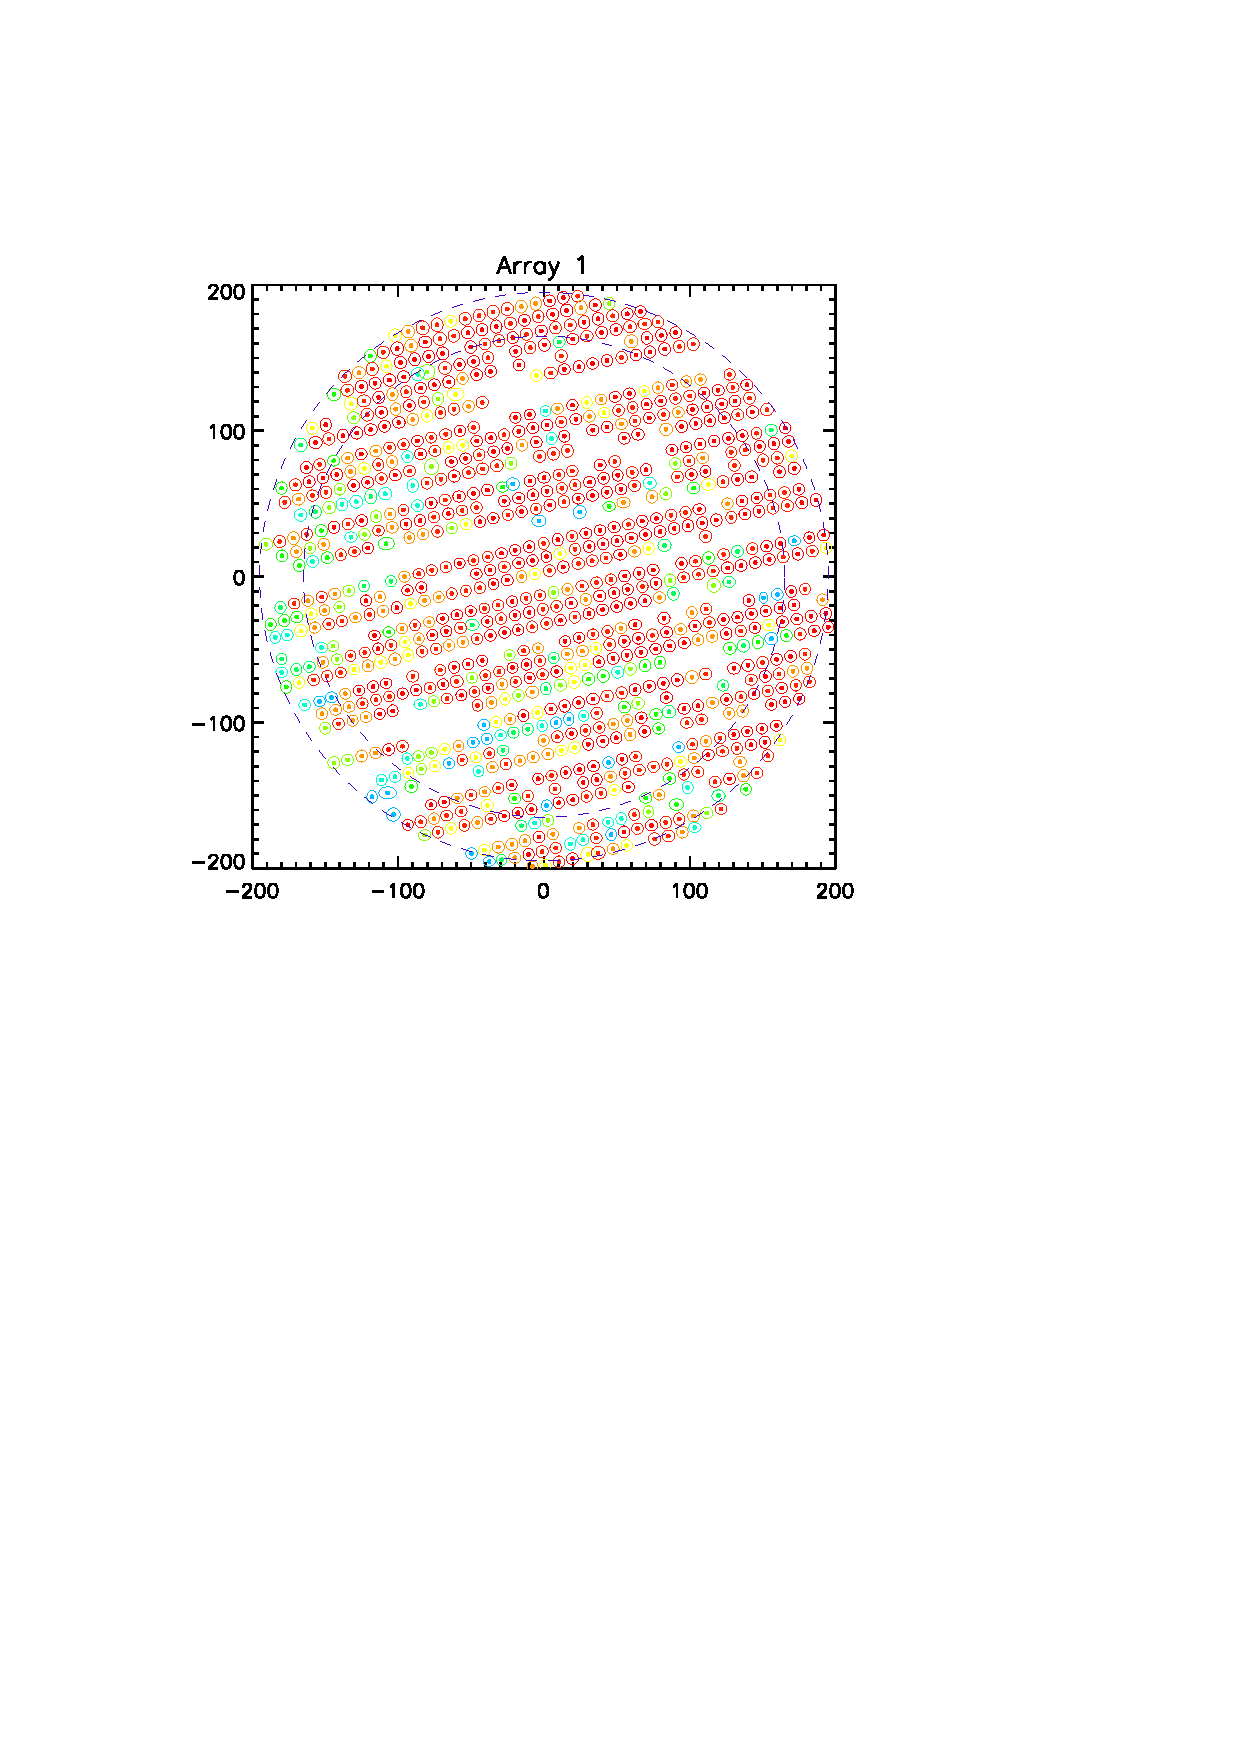
\includegraphics[trim=2cm 14cm 4cm 4cm, clip=true,width=0.55\linewidth]{Figures/A1_fwhm_color_count.pdf}
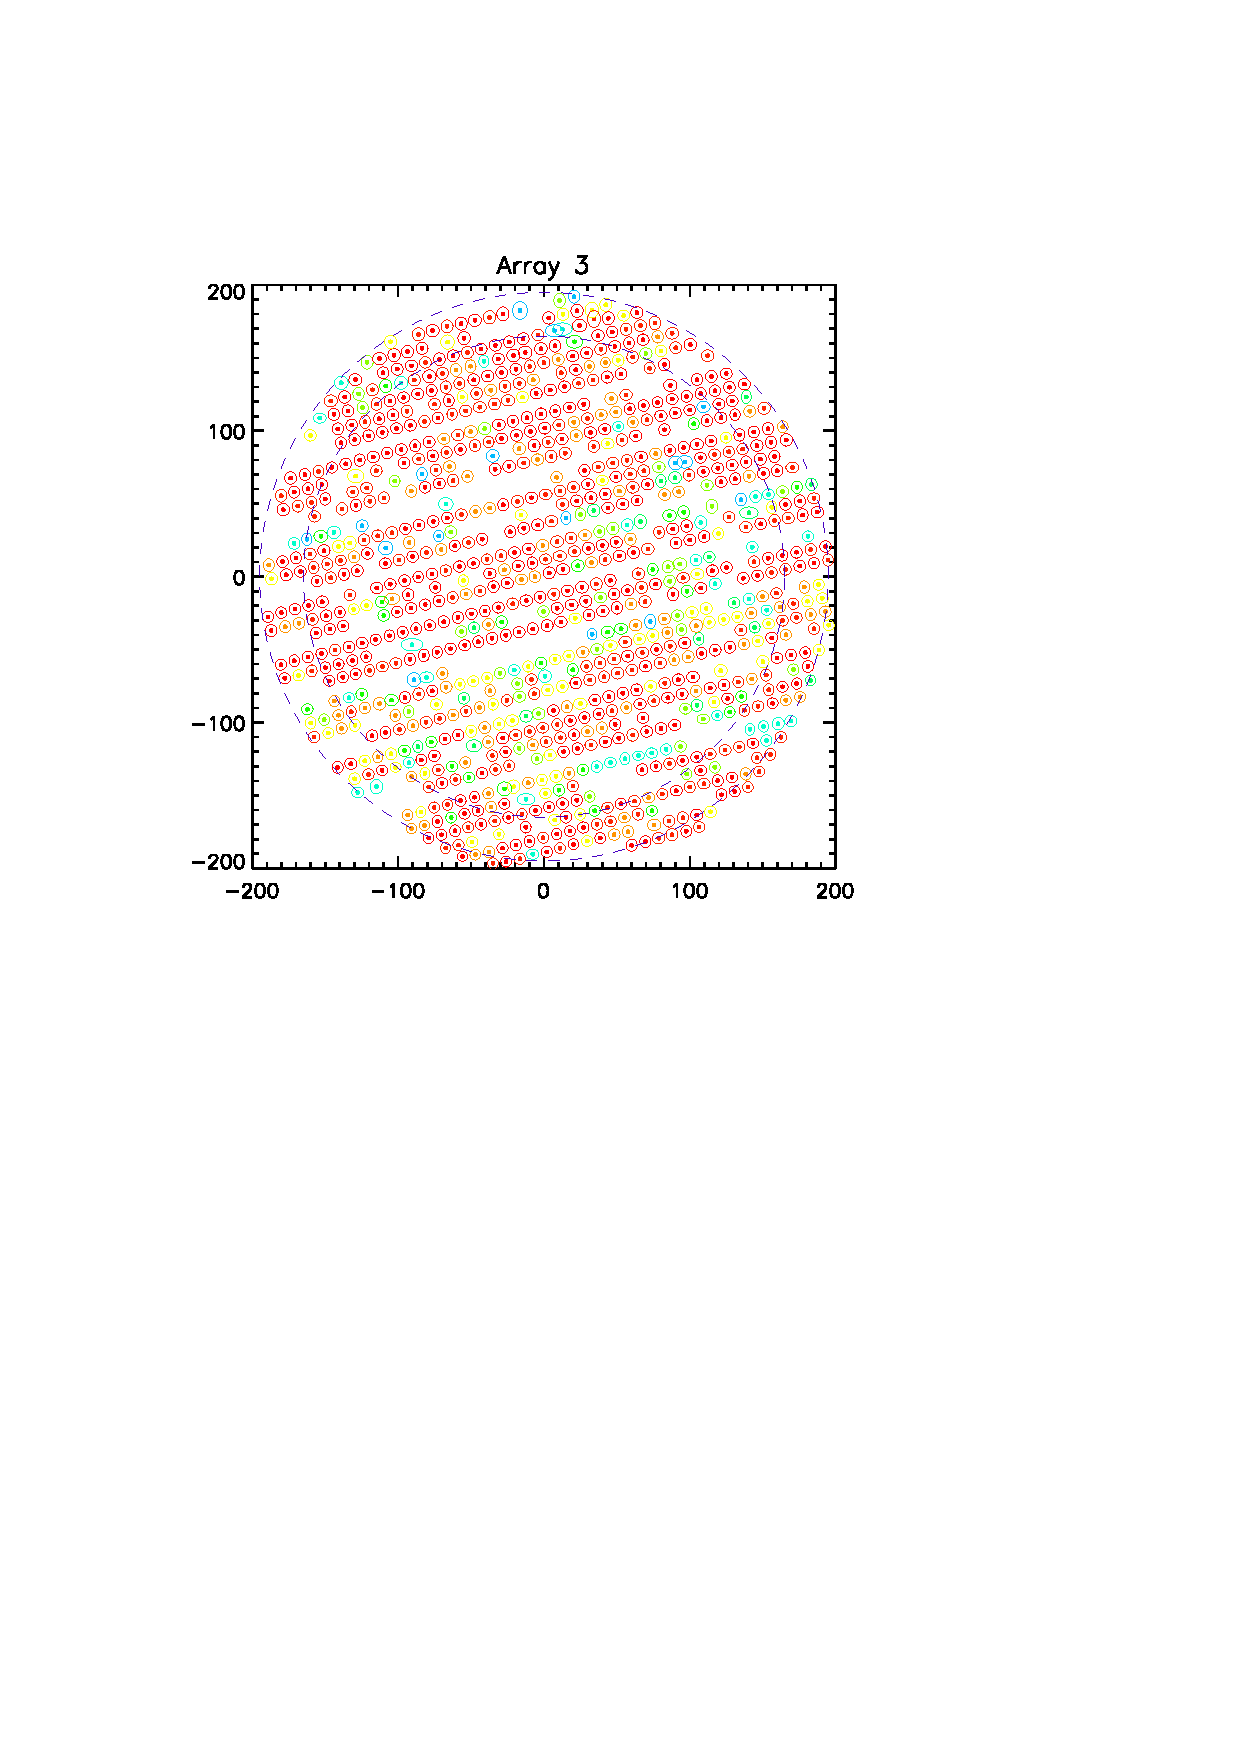
\includegraphics[trim=2cm 14cm 4cm 4cm, clip=true,width=0.55\linewidth]{Figures/A3_fwhm_color_count.pdf}
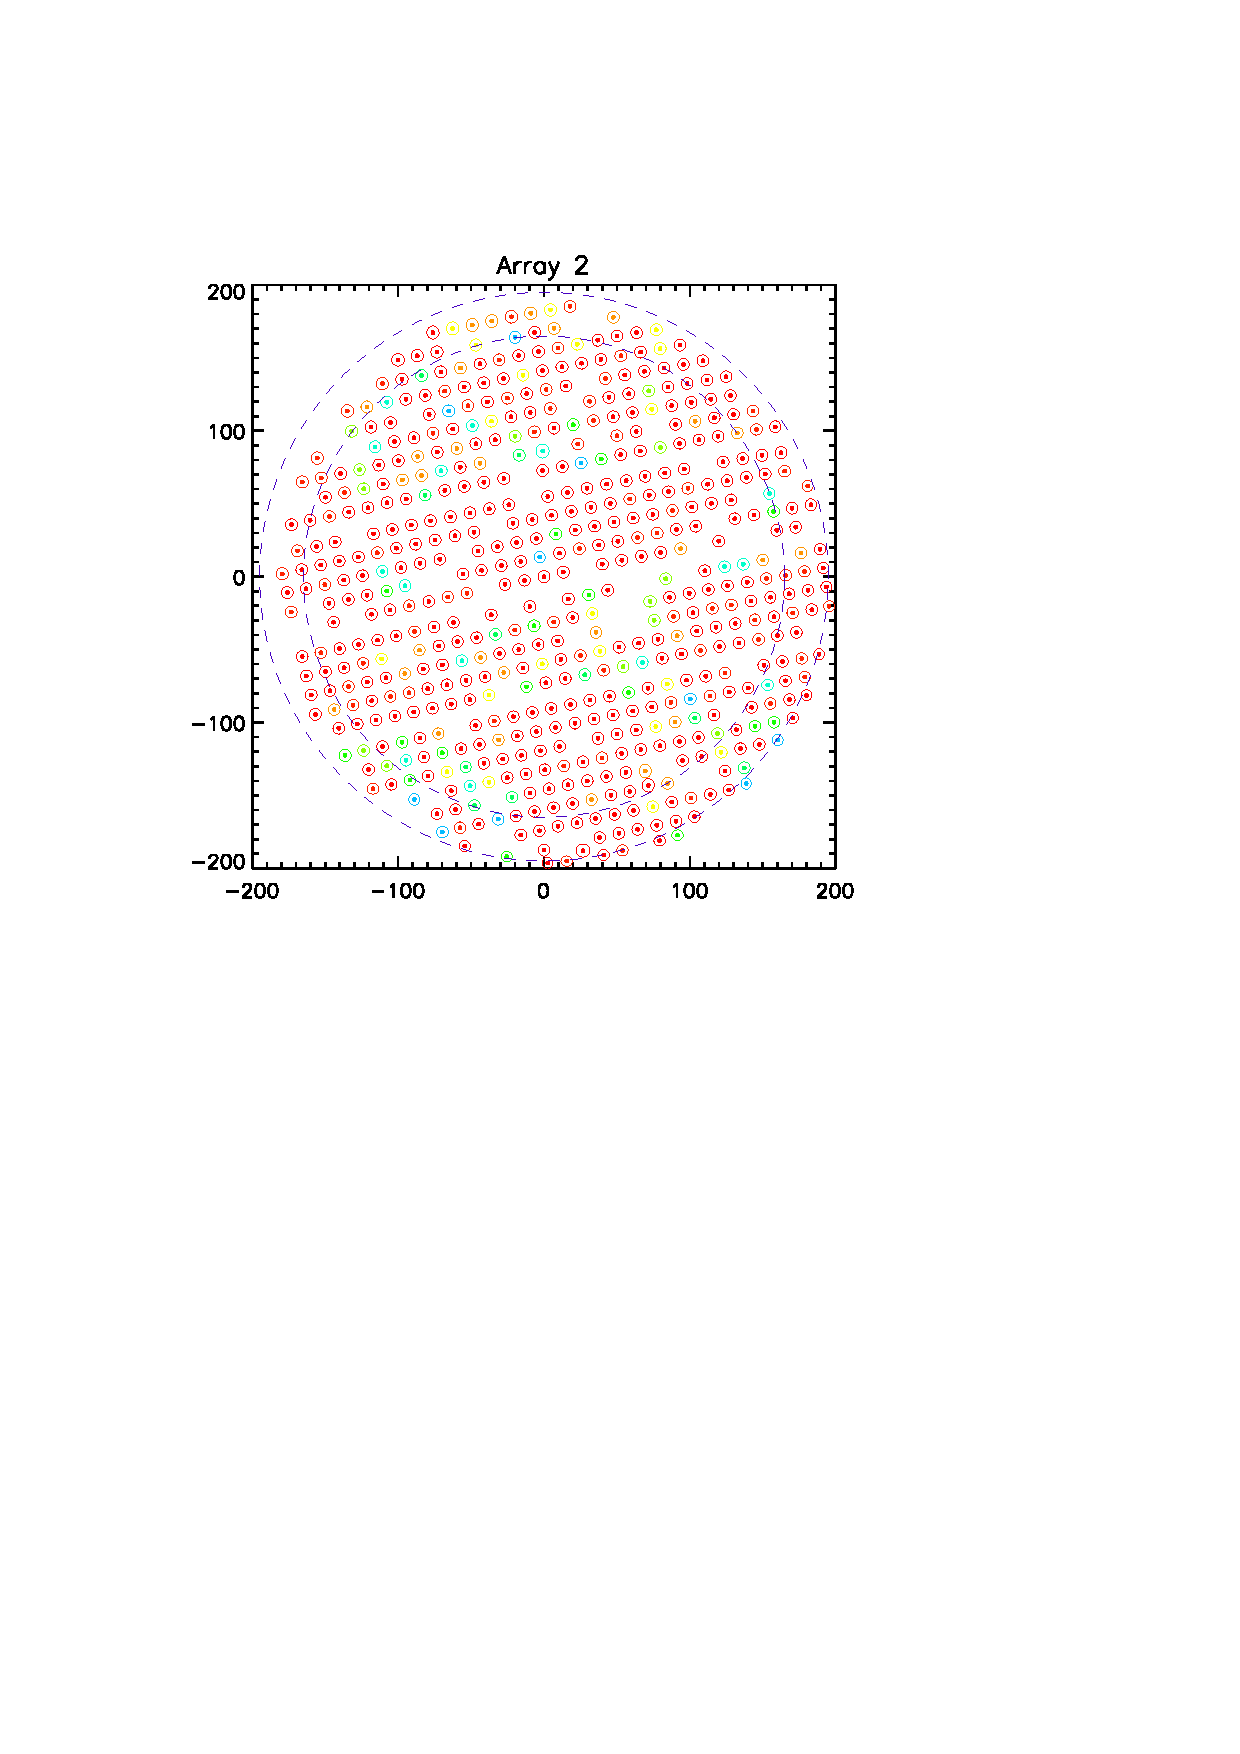
\includegraphics[trim=2cm 14cm 4cm 4cm, clip=true,width=0.55\linewidth]{Figures/A2_fwhm_color_count.pdf}
\caption{Average detectors positions for arrays A1, A3, and A2 (from
  green to red as a function of the number of times that a given pixel
  has been considered as valid). The three plots show the detectors
  that have seen the sky and passed the quality criteria for at least
  two beam maps during Run10, 9 and 8: 952, 961, and 553
  %925, 944, and 543
  for A1, A3 and A2, respectively. The inner and outer dash-line circles correspond to a 
  FOV of 5.5$\prime$ and 6.5$\prime$, respectively. Units are arcseconds. 
  The color (from green to red)  shows the number of times that a given pixel has been considered as valid.}
\label{fig:avg_fov_color}
\end{center}
\end{figure}

In order to identify the most stable pixels, we compare the KIDs parameter obtained with several beam maps. 
In the following, we   show results as obtained using seven beam maps from Run10, two from Run9 and one from Run8.
For each pixel we compute the average position on the focal plane and the average FWHM, counting the times that it has been considered as valid.

In Fig. \ref{fig:avg_fov_color} we show the average focal plane
reconstruction, from green to red depending on the number of times
that the pixel has been considered as valid. For A1, A3 and A2,
respectively, we have 952, 961, and 553 pixels that have been
considered as valid at least twice (840, 508, 868 valid at least five
times).
% LP: add a sentence to reference Table ``\ref{tab:number_of_kids}"
Using this criterion, we deduce the fraction of valid
detectors over the designed ones, as given in Table~\ref{tab:number_of_kids}. 
As a second step, we also flag pixels that move across the focal plane from a 
beam map to another (Fig. \ref{fig:jumping_kids} , jumping KIDs) and those 
who share the same position (twin KIDs). To identify the former, we look at the difference 
of the mean and median position of each KID (the red crosses and black squares in 
Fig. \ref{fig:mean_vs_median}). For the latter a criterion on the position is applied in 
order to find the pixels that are closer than the grid step.



\noindent {\bf FM: how many twins ? how many jumping kids ?}\\


\begin{figure}[htp]
\begin{center}
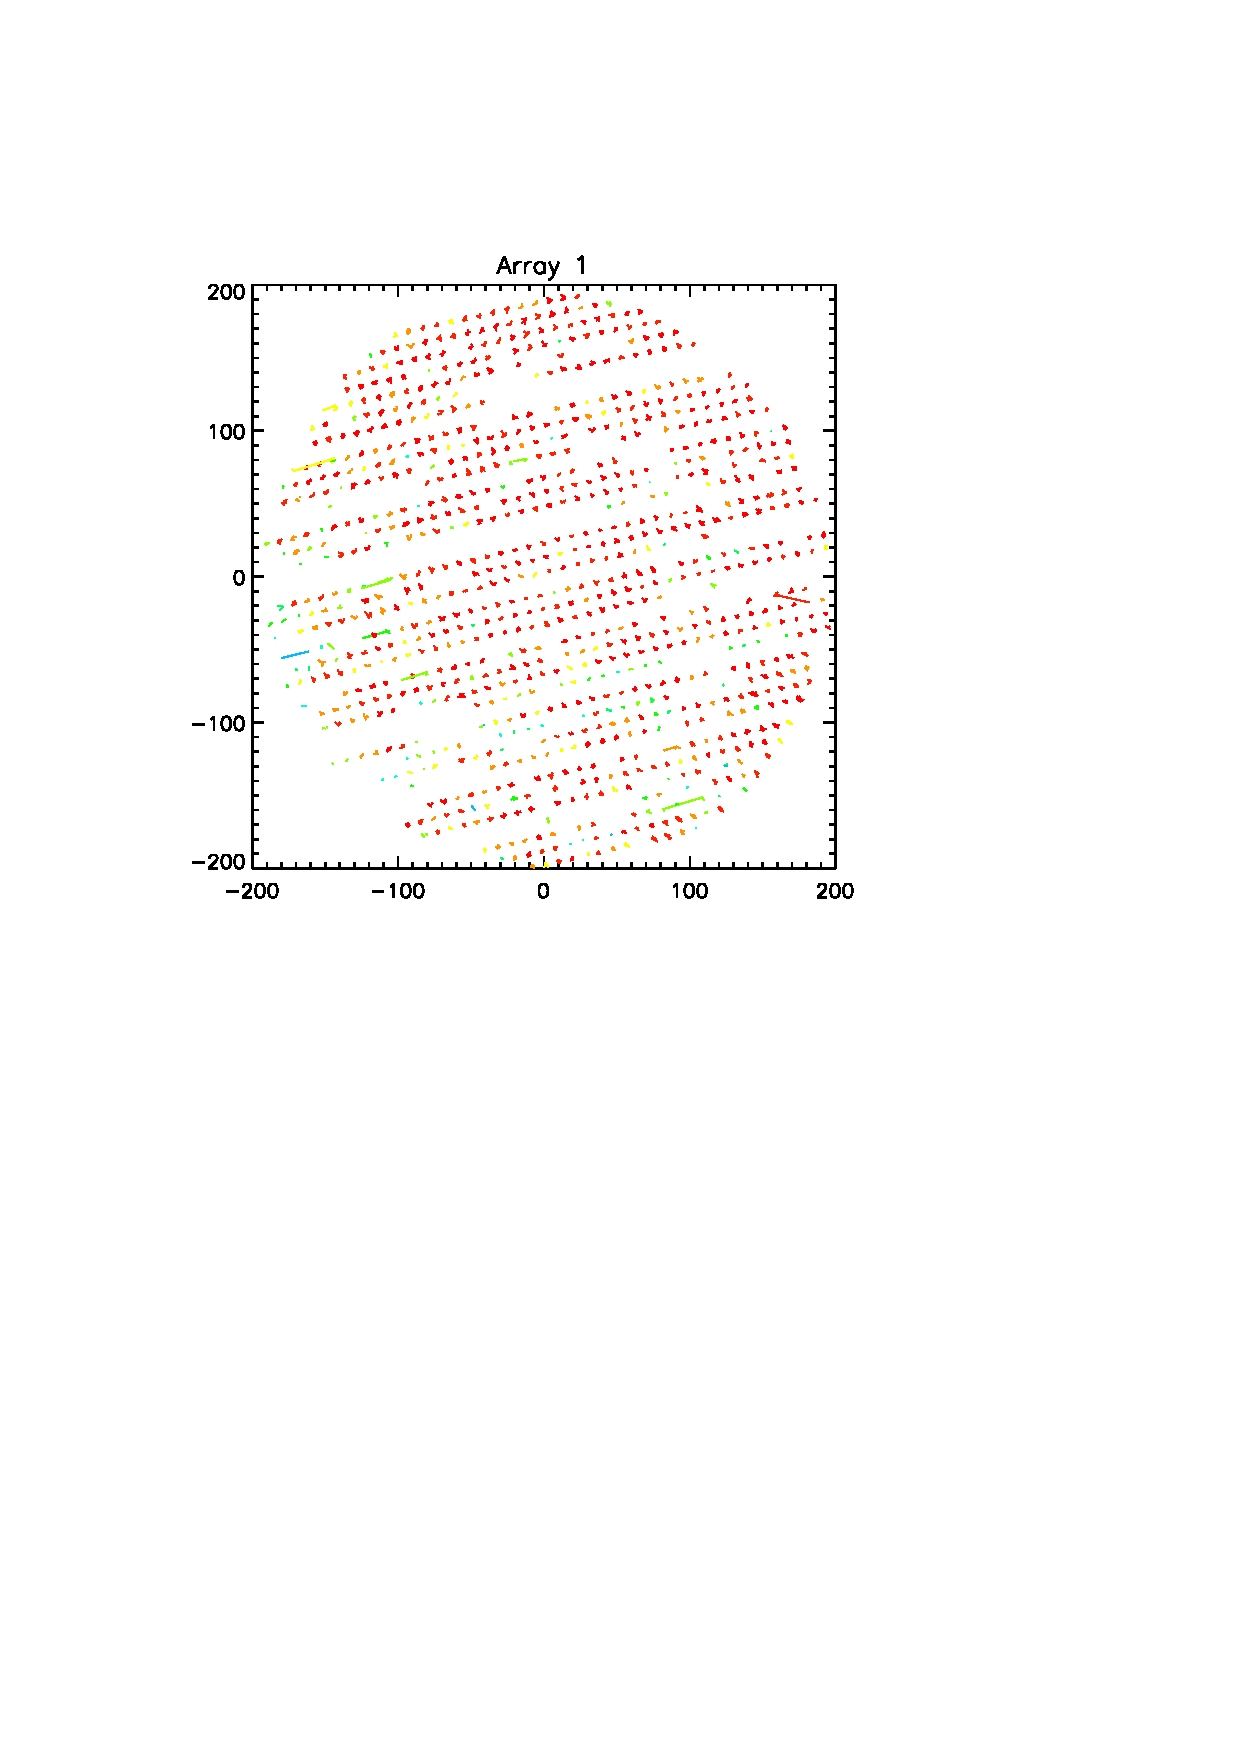
\includegraphics[trim=2cm 14cm 5cm 4cm, clip=true,width=0.55\linewidth]{Figures/A1_positions.pdf}
\includegraphics[trim=2cm 14cm 5cm 4cm, clip=true,width=0.55\linewidth]{Figures/A3_positions.pdf}
\includegraphics[trim=2cm 14cm 5cm 4cm, clip=true,width=0.55\linewidth]{Figures/A2_positions.pdf}
\caption{For the valid detectors, we show the positions of each pixel, as obtained from 
each beam map. Some of them are not found at the 
same position for all the beam maps. Units are arcseconds. {\bf FM : color code ?}}
\label{fig:jumping_kids}
\end{center}
\end{figure}

\begin{figure}[htp]
\begin{center}
\includegraphics[trim=2cm 14cm 5cm 4cm, clip=true,width=0.55\linewidth]{Figures/A1_test_positions.pdf}
\includegraphics[trim=2cm 14cm 5cm 4cm, clip=true,width=0.55\linewidth]{Figures/A3_test_positions.pdf}
\includegraphics[trim=2cm 14cm 5cm 4cm, clip=true,width=0.55\linewidth]{Figures/A2_test_positions.pdf}
\caption{For the valid detectors,
  we show the mean (red crosses) and the median (black squares)
  positions of each pixel, as obtained from each beam map.
  Units are arcseconds. {\bf FM : color code ?}}
\label{fig:mean_vs_median}
\end{center}
\end{figure}


% LP: copy from fov.tex + modif according to Samuel's comment
\begin{table}[ht]
\begin{center}  
  \begin{tabular}{|c|c|c|c|}
    \hline
    Array & Designed detectors &  Valid detectors & Fraction\\
    \hline\hline
    A1 & 1140 & 952 &  84\%\\
    A3 & 1140 & 961 &  84\%\\
    A2 & 616  & 553 &  90\%\\
    \hline
  \end{tabular}
  \caption{ CAPTION}
  \label{tab:number_of_kids}
\end{center}    
\end{table}




%   Distortion from the grid
%----------------------------------------------------------------------------------------
\subsection{FOV grid distortion}
\label{se:grid_distortion}

We studied the matching of the KIDs position on the sky to the
\emph{design} position, as decribed in detail in this wiki post\footnote{see
  {\tt http$://$www.iram.fr$/$wiki$/$nika2$/$index.php$/$}
  
  {\tt April$\_$19,$\_$2017,$\_$FXD,$\_$KID$\_$position$\_$mapping$\_$and$\_$Field$\_$distortion$\_$for$\_$Run9}
}
The global result is scaling, rotation, and shift parameters for each
array. They are described in Table~\ref{ta:gridmatch}.

\begin{table}[ht]
\label{ta:gridmatch}
\begin{center}
\begin{tabular}{|c|c|c|c|}
\hline
Array 1  &	Array 3   &	Array 2   &	Comment \\
\hline
1 mm      &       1 mm     &        2 mm  & \\
1140 	 &      1140 	   &        616  &	Total of designed Kids \\
736/673  &	758/734  &	444/437  &	Found/Well-placed Kids \\
91/59 	 &    96/64 	 &      98/71 	 & Fraction [\%] of WPK/FoundKids and WPK/Total \\
0.87 	 &     0.84 	  & 0.66     &	Median deviation (arcsec) for pixels with a deviation smaller than 5 arcsec. \\
0.52 	 &     0.69 	 &        0.68 	 & Mean distortion across the FoV in arcsec \\
2.3 -4.5  &	2.0 -5.8  &	9.3 -7.5  &	Array center in Nasmyth coordinates (arcsec) \\
4.90  &	4.88  &	4.88  &	Plate scaling (arcsec/mm) in the Design x and y (averaged) \\
77.3  &	76.4  &	78.2  &	Plate rotation angle (degree) from the Design to Nasmyth coordinates \\
6.6  &	6.6  &	6.6  &	FOV (Total kids) \\
9.8/2.00  &	9.7/2.00  &	13.3/2.75  &	Distance between near detectors [arcsec, mm] \\
1.24  &	1.22  &	0.97  &	Distance between near detectors [in lambda/D] \\
\end{tabular}
\end{center}
\caption{Linear 2D fit of the observed position of the detectors in the sky
  against their mechanical designed position for N2R9. }
\end{table}

It shows that on average the position of each detector is known to better than
an arcsecond. The 1mm arrays have almost the same center but this center
differs by 7 and 2 arseconds from the 2mm array center. The sampling is above
$\lambda/D$ at 1 mm. Note that the plate rotation angle was designed as
76.2\,degrees, less than 2 degrees from what is observed. We find that array 1
has the most deviant detectors (above 4 arcseconds from their expected
position). These detectors should be excluded from further analysis. We call
distortion (in the table) the $x.y$ term in the polynomial fitting between the
design grid and the observed position (the fitting is done with the $x$ and
$y$ linear terms and $x.y$ term). 



This has been compared to expectations obtained using ZEMAX
simulation. The grid diagram generated using ZEMAX provides us with
the maximum dispersion in the field defined by

\begin{equation}
P = \frac{\sqrt{(x_p - x_r)^2 + (y_p - y_r)^2}}{\sqrt{x_p^2 + y_p^2}},
\end{equation}

where $(x_p, y_p)$ and $(x_r, y_r)$ are respectivelly the predicted
and real coordinates on the image surface relative to the reference
field position image location (see page 170 of the ZEMAX manual, 2007).
The predicted coordinates for the whole field are obtained using a
linear interpolation of a small area in the field central part,
whereas the real coordinates are calculated by ray tracing through the
optical system.

\begin{figure}[ht] 
\begin{center}
\includegraphics[width=0.9\textwidth]{Figures/NIKA2_Final_grid.png}
\caption{NIKA2 grid diagram simulated using ZEMAX. Crosses indicate
  the real coordinates on the Nasmyth image plan. {\bf question a
    Samuel: pourquoi les dimensions indiquees sont environs 4.5 arcmin
  de cote (et pas 6.5)?}}
 \label{fig:fov_grid_distortion_zemax}
\end{center}
\end{figure}

Figure \ref{fig:fov_grid_distortion_zemax} show the ZEMAX grid diagram for
NIKA2 simulated optic system. The maximum grid distortion is expected
to be of $2.7\%$ in NIKA2 $6.5'$ FOV. The distortion is the most
noticeable in the upper right corner of the Nasmyth plan, which is
also the area of the largest defocus w.r.t. to the center. 

An expected distortion of $2.7\%$ is at most a 5 arcsecond shift from the
center to the outside of the array.  The quoted measured distortions are not
too dissimilar once the different fitting methods have been taken into
account.

% FXD: this would need to be more ascertained. Lack of time to go further.


%% [Optimal Focus]
%%________________________________________________________
\subsection{Reconstruction of the focus surfaces}
\label{sec:focus}

Owing to the NIKA2 $6.5~\rm{arcmin}$ FOV, the focus is expected to
slightly changes across the FOV, defining curved focal surfaces at the
location of the three arrays. Therefore, beam patterns are expected to
show some scatter across the FOV accordingly to the focal
surfaces. Although all the detectors cannot be individually focalised,
an optimal axial focus of the telescope can be found to maximize the
number of detectors at the best focus and hence, maximize the
resolution of the NIKA2 maps.
This optimal z-focus setting is obtained
in measuring the focus at the center of the arrays as described
Sect.~\ref{sec:focus-meas} and apply a focus shift, which is primary
predicted using Zemax simulation, and ultimately verified by measuring
the focus surfaces as decribed here.

\begin{figure}
\begin{center}
  \includegraphics[trim={0, 1cm, 0, 1cm}, clip, angle=0, scale=0.5]{Figures/fov_focus_mv_5.png}
\caption{Focus surface of A1, A3 and A2 arrays from left to
  right. From top to bottom, the focus estimates rely on
  FWHM-minimization, amplitude-maximization of an elliptical
  Gaussian of fixed FWHMs and amplitude-maximization of an elliptical
  Gaussian.}
\label{fig:focus-surfaces}
\end{center}
\end{figure}

\emph{Method. } We measure NIKA2 focal surfaces by means of a sequence of five 'beam-map'
scan observations of bright point-like sources, typically Planets or
bright quasars,
for various settings of the telescope axial focus around the
optimal focus $z_{\rm{opt}}$. A beam-map scan consists of a deep-integrated
$13.5' \times 7.8'$ OTF-scan observation comprizing $99$ sub-scans and
with a scanning speed of either $65''/s$ whenever the mean integration
elevation is $< 60$ degree or $39"/s$ at higher elevation. The z-focus is changed in step of
$0.6~\rm{mm}$ to probe a large focus range for measuring even the
extreme variation of the focus surfaces,
namely $z \in \{-1.2, -0.6, 0, 0.6, 1.2 \} + z_{\rm{opt}}$.
Each beam-map scans allow for $4''$-resolution individual maps per kid to
be projected. Before the projection, the correlated noise is mitigated
from each KID timeline in subtrating out a common mode, which is obtained
using, amongst the other detectors, those that correlates the most
with this KID and that are located outside a radius of $90''$
around the source centroid.
Therefore, a series of five cleaned maps at various focus is
available for each detector, from which the best focus is estimated as
described in Sect.~\ref{sec:focus-meas}. The ensemble of the relative
focus estimate per KIDs with respect to the best focus at the center
of the array constitutes the focus surface. An accurate estimate of
the center focus is obtained as the
weighted average focus estimate of the KIDs lying in a $30''$ radius
around the geometrical center of the array. This average does not
induce any sizeable bias thanks to the flatness of the focus surface
in the innermost regions. For robustness test, we consider three focus
estimates: the two first ones are the same as discussed in
Sect.~\ref{sec:focus-meas} -- namely i) $\hat z_{\rm{fwhm}}$ the focus that
minimizes the geometrical FWHM and ii) $\hat z_{\rm{peak}}$ the focus
that maximizes the amplitude of the best-fitting ellitical Gaussian --
whereas the third one is $\hat z_{\rm{flux}}$ the focus that maximizes
the amplitude of the best-fitting elliptical Gaussian of fixed FWHM
(at $12''$ at $260~\rm{GHz}$ and $18''$ at $150~\rm{GHz}$). The 
comparison between the two amplitude-based estimators
($\hat z_{\rm{peak}}$ and $\hat z_{\rm{flux}}$), will test the
stability of the focus results against the exact choice of the beam fitting
function. Since the ellipticity-based estimator $\hat z_{\rm{ellip}}$ is
less sensitive to focus changes and yields larger uncertainties than the
others, we do not use it for the focus surface reconstruction.     


\emph{Data selection. }
During the three commissioning campaigns that occured after the change of A1
lens and the improvement of internal optics alignment (hence in the
final NIKA2 optic configuration),
nine out-of-focus
beam-map scan sequences have been acquired, including incomplete
sequences and sequences hindered by poor atmospheric conditions. We
select sequences that i) comprises at least four scans, ii) have been
observed at zenith opacity at $225~\rm{GHz}$ (as indicated by
the IRAM taumeter) below 0.5 and iii) have a maximal central focus
drift between the starting time and the end of the sequence of
$0.5~\rm{mm}$. These criteria preserve five sequences from which focus
surfaces can be reconstructed. Namely, we consider the sequences
$20170226s415\mbox{--}419$, $20170419s133\mbox{--}137$, $20170420s113\mbox{--}117$,
$20170421s160\mbox{--}164$ and $20170424s123\mbox{--}127$, which consist of observations
of the bright quasar '3C84' and Neptune.

\emph{Results. }
For each detector $k$ and each beam-map sequence $s$, we obtain for
the array $a$, a focus measurement $z_k^{a, s} \pm \sigma_k^{a, s}$,
where $\sigma_k^{a, s}$ is the $1\mbox{--}\sigma$ error of the least-square
polynomial fit. The focus surface measurements per array obtained from the five
beam-map sequences are combined using an inverse-variance weighting
scheme to obtain the focus surface estimates 
\begin{equation}
\label{eq:mv_focus_surf}
z_k^{(a)} = \left( \sigma_k^{(a)} \right)^2 \,  \sum_s \frac{z_k^{a,s}}{\left(\sigma_k^{a,s}\right)^2}\, \,  ,
\end{equation}
with uncertainties 
\begin{equation}
\label{eq:error_mv_focus_surf}
\sigma_k^{(a)} = \left[ \sum_s \frac{1}{\left(\sigma_k^{a,s}\right)^2}\right]^{-1/2}\, .
\end{equation}


We present NIKA2 focus surfaces per arrays obtained as in
Eq.~\ref{eq:mv_focus_surf} 
%from the inverse-variance weighted combination of the five
%reconstructed focus surfaces per arrays
in Fig.~\ref{fig:focus-surfaces}.
The three flavours of focus-estimators provide us with focus surfaces
per arrays that are in good agreement with each others and that have a
non-axisymetrical flatten bowl shape consistent with expectations from
simulation {\bf [TBA, as discussed further below]}.
The median defocus (that is the relative focus w.r.t. the center)
across the detectors is about
$-0.1~\rm{mm}$ for the three arrays. Maximal defocus values of about
$-0.6~\rm{mm}$ are found for detectors located in the outer top and
left regions of the FOV. Finally, a fraction comprised between $20$
and $30\%$ of the KIDs has a relative $z\le -0.2~\rm{mm}$.  

We primarily estimate the uncertainty of the focus
surface measurements using the standard deviation between the three
estimators $z_k^{(a)}|_{\rm{fwhm}}$, $z_k^{(a)}|_{\rm{peak}}$ and
$z_k^{(a)}|_{\rm{flux}}$. We found approximatively homogeneous
standard deviation surfaces per arrays, which have median values across
the FOV of about $0.03~\rm{mm}$.
However, we cross-check this error estimate by forming the quadratic mean of
the three inverse-variance error surfaces per arrays, which are defined in
Eq.~\ref{eq:error_mv_focus_surf} and quoted
$\sigma_k^{(a)}|_{\rm{fwhm}}$, $\sigma_k^{(a)}|_{\rm{peak}}$ and
$\sigma_k^{(a)}|_{\rm{flux}}$. This provides us with more optimistic
error surfaces per array, which do not show any clear pattern across
the FOV and which have a median value across the detectors of about
$0.015~\rm{mm}$.  

%[EXPAND THE DISCUSSION ON COMPARISON WITH SIMULATION]

\emph{Stability across sequences. }
By comparing the focus surface obtained from the five individual focus
sequences, we test the stability of the NIKA2 focus surfaces across
the time and the atmospheric conditions. In
Figs.~\ref{fig:focus-stability-H}-\ref{fig:focus-stability-V}, we compare
the defocus along two perpendicular diameters across the
FOV. Although any direction would have been equivalent for this test, we choose to
position the diameters along-with and perpendicular-to the KID geometrical
grid to avoid the scatter due to KID non-alignement in any other
direction. The scatter is further mitigated by considering
four-detector-wide diameters as shown in upper the left corner of
Figs.~\ref{fig:focus-stability-H}-\ref{fig:focus-stability-V}.

{\bf add a sentence to conclude on the stability}


\begin{figure}
  %\begin{center}
  \includegraphics[trim={-2cm, 2cm, 0, 2cm}, clip, angle=0, scale=0.1]{Figures/fov_focus_stability_check_D1.png}
  \begin{center}
  \includegraphics[trim={0, 2cm, 0, 2cm}, clip, angle=0, scale=0.45]{Figures/fov_focus_1D_Vband_5.png}
  \end{center}
  \caption{Stability of the focus surface across the sequences. This
    series of plot show the relative focus with respect to the center
    (defocus) along the 'vertical diameter', that is a band of
    four-detector width across the FOV, which is vertical with respect to
    the detector geometrical grid, as illustrated by the plot in the
    upper left corner. The datapoints show the defocus along the
    'vertical diameter' estimated from the five focus sequences,
    namely $20170226s415\mbox{--}419$ (sky blue),
    $20170419s133\mbox{--}137$ (dark blue), $20170420s113\mbox{--}117$ (red),
    $20170421s160\mbox{--}164$ (yellow) and $20170424s123\mbox{--}127$
    (green), using the $z^{(a)}|_{\rm{fwhm}}$, $z^{(a)}|_{\rm{flux}}$ and
    $z^{(a)}|_{\rm{peak}}$ estimators from top to bottom, and for A1, A3 and
    A2 arrays from left to right. The black datapoints are the five-sequence combined defocus, as
    presented in Fig.~\ref{fig:focus-surfaces}, taken along the
    'vertical diameter', and the errorbars, the
    five-sequence combined defocus errors along the 'vertical
    diameter'.}
\label{fig:focus-stability-H}
\end{figure}


\begin{figure}  
  \begin{center}
  \includegraphics[trim={0, 2cm, 0, 2cm},clip, angle=0, scale=0.45]{Figures/fov_focus_1D_Hband_5.png}
  \caption{Stability of the focus surface across the sequences. Same
    legend as in Fig.~\ref{fig:focus-stability-H}, but for the
    detectors located in an 'horizontal diameter', i.e. a band of
    four-detector width across the FOV, which is horizontal with respect to
    the detector geometrical grid, as illustrated by the plot in the
    upper left corner. }
\label{fig:focus-stability-V}
\end{center}
\end{figure}



% + Focal Plane Geometry
% + KID selection and average geometry
% + FOV grid distortion
% + Reconstruction of the focus surfaces


\clearpage
%----------------------------------------------------------------------------------------
%	BEAM PATTERN
%----------------------------------------------------------------------------------------
\section{Beam pattern}
\label{se:beams}
%%
%%
%%      SECTION: BEAM PATTERN 
%%

%% [intro]
%%________________________________________________________

The NIKA2 beam pattern mainly depends on the IRAM 30m telescope and NIKA2 internal optical system characteristics, whereas the detectors themselve might have an impact at sub-dominant level (through e.g. time constants or correlated noises). In this section, first we reconstruct the focus surfaces and present the optimal focus, then we characterize both the main beam, which is modeled as an elliptical Gaussian, and the full beam pattern including error beams up to angular scales of 10 arcmin. 

%% [Optimal Focus]
%%________________________________________________________
\subsection{Optimal focus}

\subsubsection{Focus estimation}

[DESCRIPTION NK-OTF-FOCUS + 1 FIG. D'EXEMPLE]

\subsubsection{Reconstruction of the focus surfaces}

[DESCRIPTION BEAMMAP SEQUENCE + FIGS]


%% [Main beam]
%%________________________________________________________
\subsection{Main beam}

For NIKA2 main beam characterization, we use \emph{Run9} OTF scans of bright point sources, including primary and secondary calibrators. Namely, we consider scans of Uranus, Neptune, 3C273, 3C84, 0316+413, Vesta and MWC349, whereas we avoid CRL2688 and NGC7027, which are slighltly extended. We perform a conservative data selection from the observing conditions by demanding average elevations $\rm{el} \ge 20°$, zenith opacities as estimated by NIKA2 in the 1mm band $\tau_{1\rm{mm}} \le 0.4$, reasonable lateral focus settings $x, y \le 0.5$mm. After selection cuts, our data set includes 130 OTF scans, which consists of a representative sub-sample of a typical NIKA2 observation campaign.    

  
We consider different methods for the main beam characterization: i) Gaussian fits of the beam profile to benefit from the signal-over-noise increase after azimuthally averaging the signal, ii) Elliptical Gaussian fits of the beam map for a better 2D modeling. Cross-checking the outputs from these complementary methods is an important robustess test of our results.   


\subsubsection{profile-based analysis}

[JEAN-FRANCOIS]

\subsubsection{map-based analysis}

NIKA2 main beam two-dimensionnal distribution is modeled using an elliptical Gaussian. We characterize NIKA2 resolution by giving the \emph{FWHM}, defined as
\begin{equation}
  FWHM = 2 \sqrt{2\ln {2}} \sqrt{\sigma_x\sigma_y},
\end{equation}
where $\sigma_x$ and $\sigma_y$ are the Gaussian standard deviation along minor- and major-axis. To avoid the side lobes contamination, we use masked versions of the beam map, in which an annulus of inner radius $r_{\rm{in}}$ and outter radius $r_{\rm{out}}$ is cut out. Whereas $r_{\rm{out}}$ is conservately set to be $100 arcsec$, $r_{\rm{in}}$ can vary to provide the best 2D Gaussian fit. We checked a posteriori that $r_{\rm{in}}$ distributes as $7 \pm 1.5$ arcsec at 1mm and $13 \pm 4$ arcsec at 2mm, in agreement with settings defined in the profile-based analysis.   

Figure~\ref{fig:fwhm_map} shows FWHM distributions obtained from the elliptical Gaussian fit method.


\begin{figure}
\begin{center}
  \includegraphics[clip, angle=0, scale=0.4]{Figures/plot_histo_fwhm_run9_calibII_all_nocut.pdf}
\caption{Distribution of the FWHM estimates using 2D Gaussian fits on \emph{N2R9} OTF scans of brigth point sources}
\label{fig:fwhm_map}
\end{center}
\end{figure}


The FWHM estimates using the profile-based and map-based methods are gathered in Tab.~\ref{tab:fwhm}. 
\begin{table}
  \caption[]{FWHM of the NIKA2 main beam in arcsec.}
  \centering
  \begin{tabular}{|l|l|l|l|l|}
    \hline
    Array & profile-based method & map-based method \\
    \hline
    A1       & [TBC] & $11.0 \pm 0.3$ \\
    A3       & [TBC] & $10.9 \pm 0.3$ \\
    A1 \& A3 & [TBC] & $11.0 \pm 0.2$ \\
    A2       & [TBC] & $17.8 \pm 0.2$ \\
    \hline
  \end{tabular}
  \label{tab:fwhm}
\end{table}



%% [Full beam pattern]
%%________________________________________________________
\subsection{Full beam pattern}

\subsubsection{Deep beam maps}
We present the two-dimensional distribution of the beam in Fig.~\ref{fig:beam}. We primary use a map obtained from a combination of deep observations of strong point sources collected during \emph{NIKA2-run8} and \emph{run9}. Namely, we use 'beammap' OTF scans of Uranus (scan id '20170125s223' and '20170125s243'),  Neptune ('20170224s177') and the bright quasar 3C84 ('20170226s415'). However, we checked the stability of our results on single scan maps, combinations of scans for a single source, and combinations of shallower scans but spanning a large range of scanning direction. The data processing includes a mitigation of the correlated noise, which mainly originates from the atmosphere.  We primarly use a subtraction of a common mode estimated from the most correlated detectors (the so-called 'cm one block' method). However, other methods are tested for assessing the immunity of our results to noise residuals.

\begin{figure}
\begin{center}
  \includegraphics[clip, angle=0, scale=0.4]{Figures/Lobe_map_Combo_v2_dB.pdf}
 \caption{Beam pattern. From upper left to lower right, beam maps of array 1 (labeled 'A1'), array 3 ('A3'), the combination of the 1.15mm arrays ('A1$\&$3') and the 2mm array ('A2') are shown in decibel. These maps, which consist of normalized combination of four long OTF scans of bright point sources, are in celestial coordinates and cover a sky area which extend over 10 arcmin.}
\label{fig:beam}
\end{center}
\end{figure}


The deep NIKA2 beam maps reveal some noticeable features, which are shown in Fig.~\ref{fig:features}. 

\begin{figure}
\begin{center}
  \includegraphics[clip, angle=0, scale=0.4]{Figures/Beams_features.pdf}
\caption{Noticeable features of NIKA2 beam pattern. Red circle: diffraction ring seen in 1-mm maps (the spokes are presumably caused by radial and azimuthal panel buckling (cf. Fig.4 in Greve et al. 2010)); Perpendicular green lines: diffraction pattern caused by quadrupod secondary support structure (prominently seen in 2mm maps); Yellow arrows in the upper right pannel: pattern of 3 spikes seen in 1mm maps of unknown origin; Yellow arrows in the lower right pannel: four symmetrical spokes of the first errorbeam; Pink ellipses: 4 spikes seen in 2mm maps.}
\label{fig:features}
\end{center}
\end{figure}

We further quantify the relative level of the main beam, the first error beam and other features seen in the 2D beam pattern using radial cuts.

[FIGURE JEAN-FRANCOIS]

\begin{figure}
\begin{center}
\includegraphics[clip, angle=-90, scale =0.3]{Figures/Array_A1_dB.pdf}
\includegraphics[clip, angle=-90, scale = 0.3]{Figures/Array_A2_dB.pdf}
\includegraphics[clip, angle=-90, scale = 0.3]{Figures/Array_A3_dB.pdf}
\caption{Two orthogonal cuts through the beam are shown in red and green and a best fit model made
of three Gaussians is superimposed in black. These cuts were obtained from the high quality map of Uranus on 2017 January 25th.
The main beam starts to depart from the first Gaussian at -12dB. }
\label{fig:beam_dB3}
\end{center}
\end{figure}

The Iram 30-m beam as seen with NIKA2 is shown in
Fig. \ref{fig:beam_db} by means of two orthogonal cuts through Uranus
from a high quality map obtained on 2017 January 25th in excellent conditions
(low opacity $\tau_{225}=0.08$ and elevation $46^{\circ}$).
A model made of three Gaussians centered on the source peak was best
fit {\it by hand} to these cuts and the parameters are reported in
Table \ref{tab:3gauss} [PEUT-ETRE AVANTAGEUSEMENT REPLACED PAR VALEURS DE FLORIAN].
The main beam starts to depart from the first
Gaussian at the level of about -12dB for the three arrays.
We note that for the instrument EMIR on the radiotelescope,
this departure is about -20dB (Kramer, Penalver and Greve 2013).
From parameters in Table \ref{tab:3gauss}, one can estimate that
the source incident power is split about equally between the main beam
and the error beam at 1mm, and these fractions are 70\% and 30\% at 2mm, respectively.
This modelling uses the central
region   $180'' \times 180''$ in size with a uniform noise rms from
a larger area of 8' x 5' on the sky scanned with the arrays. It is expected
that the error beam extend beyond these limits.


\begin{table}
\centering 
\caption[]{Model parameters of the three Gaussian beam.}
\begin{tabular}{|l|l|l|l|l|l|l|}
\hline
               & \multicolumn{3}{c|}{A1 and A3} & \multicolumn{3}{c|}{A2}  \\
\hline
fwhm      & $11.25''$ & $45''$  & $250''$ & $17.75''$ & $56''$  & $420''$ \\
amplitude & 0.984     & 0.015   & 0.0005   &  0.9875   & 0.011   &  0.0005\\
\hline
\end{tabular}
\label{tab:3gauss}
\end{table}


\subsubsection{Beam profile}

\begin{figure*}[h!]
\centering
\includegraphics[height=6cm]{Figures/Beam_profiles_A1_FR.pdf}
\hspace{0.5cm}
\includegraphics[height=6cm]{Figures/Beam_profiles_A2_FR.pdf}
\hspace{0.5cm}
\includegraphics[height=6cm]{Figures/Beam_profiles_A3_FR.pdf}
\caption{{\footnotesize Beam profiles for array 1, 2, and 3.}}
\label{fig:beam_profiles_3G}
\end{figure*}


\subsubsection{Beam efficiency}


%% [STABILITY]
%%________________________________________________________
\subsection{Stability of the beam pattern}

[A FAIRE:

  AJOUTER LES PLOTS DE STABILITE EN FONCTION DE ELEVATION, TAU

]




% Full Beam Pattern
% Main Beam
% Stability of the Beam Pattern


\clearpage
%----------------------------------------------------------------------------------------
%	INTER-CALIBRATION
%----------------------------------------------------------------------------------------
\section{Flat-fielding}
\label{se:flat_field}

\subsection{Inter-calibration {\color{blue} Nico}}
\label{se:intercalibration}

{\color{blue} More details on the intercalibration as described in Sect.~\ref{se:fp_reconstruction}} \\

{\color{blue} NB: Main beam flat field = calib $\_$ fwhm $\_$ fix}


\subsection{Flat field stability {\color{blue} Laurence} }
\label{se:flatfields}

The dispersion of the detector responsivity across the field of view has been characterized by estimating flat fields using the nominally focused \emph{beammap} scans described in Sect.~\ref{se:fp_reconstruction}. We have considered different kinds of flat field:
\begin{itemize}
\item Main beam flat field: the flat field for the main beam, which is the far field of the telescope estimated for the sources, is determined using the relative calibration factors obtained for the calibration in FWHM$_{0}$ beam discussed in Sect.~\ref{se:cal_HA}. These are defined as
  \begin{equation}
    G_k = \frac{S_{th}(\nu_0)\, e^{-\tau/sin(\delta)}}{A_k}, 
  \end{equation}
  where $S_{th}(\nu_0)$ is the expected flux of the source integrated in the NIKA2 bandpasses and derived at the reference frequency $\nu_0$, $\tau/sin(\delta)$ is the line-of-sight opacity measured using the \emph{skydip} method described in Sect.~\ref{se:opacities} and $A_k$ is the amplitude of a Gaussian of fixed FWHM fitted from the detector $k$ map (as $A_{c}$ in Eq.~\ref{eq:calib_fix_fwhm}).
\item Forward beam flat field: the flat field for forward beam, which is the near field of the telescope determined for the sky noise, is estimated using the correlation factor of each detector to a median common mode estimated off-source.
\end{itemize}

Figures \ref{fig:avg_mbff} and \ref{fig:avg_fbff} show the average main beam and forward beam flat fields for the three arrays. These have been constructed by combining the normalised flat fields of five \emph{beammap} scans, which were selected by thresholding the line-of-sight opacity measured in the 1-mm band, such as $\tau/sin(\delta) \leq 0.85$. The distribution for the average flat fields are shown in the bottom panel of Fig.~\ref{fig:avg_mbff} $\&$ \ref{fig:avg_fbff}.

We observe a sizable variation of the flat fields for Array 1 from the left-most side to the right-most side of the FOV: this reveals a significant change of Array 1 detector responsivities depending on their position in the FOV. Namely, this effect, the origin of which is under investigation, mainly impacts the left-most third of the array, which is referred to as the "shadow-zone''. This variation of the flat field tanslates into a broadening of the distribution. However, we verified that A1 flat field dispersions are in line with the ones of Array 3 after the detectors within the shadow-zone were flagged out using a crescent-shaped mask. The masked flat field distributions are shown in green in Fig.~\ref{fig:avg_mbff} $\&$ \ref{fig:avg_fbff}, whereas shadow-zone distributions are in red. In addition to the average flat fields, we further characterize the flat fields for individual \emph{beammap} scans. Fig.~\ref{fig:stddev_ff} shows the dispersion of the flat fields for nine \emph{beammap} scans using either the whole FOV or masking the shadow-zone. The dispersion estimates for this two cases are gathered in Table~\ref{tab:flatfields}.      

\begin{table}[h]
\begin{center}
\begin{tabular}{|l|l|c|c|c|}
\hline
 Dispersion ($\%$)    & KID selection  &  A1 & A3  & A2 \\
\hline
Main beam flat field  & all the FOV           & $34.4 \pm 3.4$    & $15.5 \pm 1.4$  &  $13.2 \pm 1.7$  \\
                      & shadow-zone excluded  & $17.0 \pm 1.1$    & $14.2 \pm 1.2$  &  $12.8 \pm 1.3$\\
\hline
Forward beam flat field  & all the FOV           & $21.6 \pm 1.4$  & $10.1 \pm 1.7$  & $5.2 \pm 0.9$   \\
                         & shadow zone excluded  & $12.2 \pm 1.6$  & $10.1 \pm 2.1$  & $4.9 \pm 1.2$ \\
\hline
\end{tabular}
\caption[Flat field dispersions]{Average flat field dispersions in percent for nine \emph{beammap} scans over all the FOV and after masking out the shadow-zone}
\end{center}
\label{tab:flatfields}
\end{table}


\begin{figure}[ht] 
\begin{center}
  \includegraphics[width=0.95\textwidth]{Figures/FlatFields/Average_main_beam_flat_field_N2R9_10.png}
  \includegraphics[width=0.8\textwidth]{Figures/FlatFields/Histo_average_main_beam_flat_field_N2R9_10.png}
\caption{Average main beam flat field for array 1, 3 and 2}
 \label{fig:avg_mbff}
\end{center}
\end{figure}

\begin{figure}[ht] 
\begin{center}
  \includegraphics[width=0.95\textwidth]{Figures/FlatFields/Average_near_beam_flat_field_N2R9_10.png}
  \includegraphics[width=0.8\textwidth]{Figures/FlatFields/Histo_average_near_beam_flat_field_N2R9_10.png}
\caption{Average forward efficiency flat field for array 1, 3 and 2}
 \label{fig:avg_fbff}
\end{center}
\end{figure}

\begin{figure}[ht] 
\begin{center}
  \includegraphics[width=0.6\textwidth]{Figures/FlatFields/Dispersion_main_beam_flat_field_N2R9_10_.png}
  \includegraphics[width=0.6\textwidth]{Figures/FlatFields/Dispersion_forward_beam_flat_field_N2R9_10_.png}
\caption[Dispersion of the flat field for nine \emph{beammap} scans.]{The RMS dispersion of the main beam flat field (upper panel) and forward beam flat field (lower panel) are shown using all valid KIDs of Array 1 (red circles), Array 3 (orange circles) and Array 2 (blue circles), and using the KIDs located outside the Array 1 "shadow area'', which was discarded using a left crescent-shaped mask (red crosses).}
 \label{fig:stddev_ff}
\end{center}
\end{figure}




\clearpage
%----------------------------------------------------------------------------------------
%	ABSOLUTE CALIBRATION
%----------------------------------------------------------------------------------------
\section{Absolute calibration}
\label{se:calibration}

% Paragraphe Intro
% NIKA2 Photometric System
%
%%
%%
%%

%% [intro]

The calibration of the NIKA2 instrument in its final configuration
of January 24th 2017  is studied in this section  in using the 
 primary calibrators, Uranus and Neptune, and secondary calibrators ; the two largest asteroids Ceres and Vesta, and the three
planetary nebulae NGC7027, CRL2688, and MWC349.


% HA 
\subsection{NIKA2 Photometric System}
\label{se:cal_HA}

\begin{table}[h]
\begin{center}
\begin{tabular}{|c|c|c|}
\hline
     & 1 mm & 2 mm \\
\hline
Reference frequency $\nu_{0}$ & 260 GHz & 150 GHz \\
\hline
Reference FWHM                      & 12.5  '' & 18.5 '' \\
\hline
\end{tabular}
\caption{NIKA2 reference frequencies and FWHM}
\end{center}
\label{tab:definitions}
\end{table}

\subsubsection{Response of a detector to astronomical source}

\noindent {\bf FM: airmass was $x$ in previous section, and elevation was $\delta$. we have to choose among these various notations}\\

Let us consider a source observed at airmass $\sec z$ under
$mm_{H_{2}O}$ of precipitable water, with specific intensity $I_{\nu}$ (in units
of  ${\rm W/m^{2}/sr/Hz}$) in the direction $\theta, \phi$, where $\theta$
is the off-axis distance and $\phi$ the position angle, illuminating a KID
of the NIKA2 array. 

A KID response located at position $\theta, \phi$
on the focal plane to this signal will be:
\begin{equation}
R(\theta, \phi, \sec z, mm_{H_{2}O}) = G_{k} \int_{0}^{+\infty} I(\nu)
\frac{T'(\nu)}{\left(\frac{\nu}{\nu_{0}}\right)^{2}} e^{\left(-\sec z
  . \tau(\nu,  mm_{H_{2}O})\right)}A\Omega (\nu)  d\nu 
\label{eq:basicphot}
\end{equation}

\noindent {\bf FM: if $k$ is the kid number, then it should be $R_k$}

where the different factors in the integral are:
\begin{itemize}
\item $\frac{T'(\nu)}{\left(\frac{\nu}{\nu_{0}}\right)^{2}}$:  the
  system transmission. $T'(\nu)$ is the transmission as measured in
  section~\ref{se:bandpasses} with a Rayleigh-Jeans source. It is
  divided by $\left(\frac{\nu}{\nu_{0}}\right)^{2}$ to correct for the
  incident spectrum.
   
   \noindent {\bf FM: in section 2, we define $T$ note $T^\prime$}\\

\item $e^{\left(-\sec z . \tau(\nu,  mm_{H_{2}O} )\right)}$: the
  atmospheric transmission at airmass  $\sec z$ for an amount of
  precipitable water vapor $mm_{H_{2}O}$ generating an opacity $\tau(\nu)$.
\item $A\Omega (\nu) $: the KID etendue   {\bf FM: extent ? etendue is not english as far as i know}, {\it i. e.} the product of
  its light collecting area by the solid angle it intercepts on the
  sky. While the step between  pixels is well known and is measured (see sec~\ref{se:fov}), the
  actual solid angle is not known precisely and is {\em probably} a function of the
  frequency  because the pixels sizes are close to the wavelength of
  operation (2.75 mm at 2mm for example). The collecting $A$ area is the
  projection of the IRAM primary on the cold pupil and is also not
  known very accurately.
\end{itemize}
The integral in eq~\ref{eq:basicphot} gives the total power (units of $\rm W$)
falling on a pixel. The factor $G_{k}$ (units of  $\rm W^{-1}$) converts this
power to ADU. {\bf FM:  ADU ?}

By virtue of the conservation of specific intensity in a telescope,
equation~\ref{eq:basicphot} can be rewritten as:
\begin{equation}
R(\theta, \phi, \sec z, mm_{H_{2}O}) = G_{k} A_{p}\Omega_{s}\int_{0}^{+\infty} I(\nu)
\frac{T'(\nu)}{\left(\frac{\nu}{\nu_{0}}\right)^{2}} e^{\left(-\sec z
  . \tau(\nu,  mm_{H_{2}O})\right)} \Omega_{b} (\theta, \phi, \nu)  d\nu 
\label{eq:basicphot2}
\end{equation}
where:
\begin{itemize}
\item $A_{p}$ is the area of the entrance pupil ({\it i.e.} the
  dish collecting area).
\item $\Omega_{s}$ is the solid angle of the source seen from the
  entrance pupil.
\item $\Omega_{b}(\theta, \phi, \nu)$ is the fraction of source signal
  illuminating the KID. It is thus normalized so that:
\begin{equation}
\int\int_{4\pi} \Omega_{b}(\theta, \phi, \nu) \sin \theta d\theta
d\phi = 1 
\label{eq:omegabdef}
\end{equation}
\end{itemize}

Equation~\ref{eq:basicphot2} describe the response of a KID, and it
is quite complex. We will in the following simplify it by making a few
assumptions. Let us first turn ourselves toward the effect of the
atmosphere. 


\subsubsection{Effect of the atmosphere}

In order to study the effects of the atmosphere, let us define the
effective frequency of a source as the weighted frequency of the
passband, taking into account the system and atmospheric transmission,
as well as the shape of the incident spectrum:
\begin{equation}
\nu_{eff}( \sec z, mm_{H_{2}O}) = \frac{ \int_{0}^{+\infty} I(\nu) \frac{T'(\nu)}{\left(\frac{\nu}{\nu_{0}}\right)^{2}} e^{\left(-\sec z
  . \tau(\nu,  mm_{H_{2}O})\right)} \nu d\nu } { \int_{0}^{+\infty} I(\nu) \frac{T'(\nu)}{\left(\frac{\nu}{\nu_{0}}\right)^{2}} e^{\left(-\sec z
  . \tau(\nu,  mm_{H_{2}O})\right)}  d\nu}
\label{eq:nueff}
\end{equation}
In order to compute the atmospheric tramission, we have used
the IRAM atmosphere 2009 models provided in GILDAS, computed for
'midlatwinter' conditions, a temperature of 268 K  and a pressure of 703.5
hPa. $\nu_{eff}$ allows to characterise the impact of the variation of
the atmospheric transmission on the full system transmisison.  Note
that the instrument transmission $T'(\nu)$ is the one measured in
sec~\ref{se:bandpasses}. 

Figure~\ref{fig:nueff} shows the variations of
$\nu_{eff}$ as a function of the water content of the atmosphere for
two elevations (zenith and 20 degree) and two spectral shape (RJ and
flat spectrum), in the two 1mm passbands and in the 2mm passband. 

Typical variations of $\nu_{eff}$ with the spectral shape of the
source range between 1\% and 3\%, and are relatively stable between good
($\tau_{225GHz} \simeq 0.1$) and
poor  ($\tau_{225GHz} \simeq 1.0$) atmospheric conditions for both the
1mm and 2mm bands. 


Let us now examine the effect of elevation.
Under good atmospheric conditions ($\tau_{225GHz} \simeq 0.1$), $\nu_{eff}$ change by
less than 0.3\% betwen zenith and 20 degree elevation. Under poor
conditions ($\tau_{225GHz} \simeq 1.0$), this rises to almost 3\% for
a Rayleigh-Jeans spectrum in the 2mm band, {\it i.e.} larger than the
  variations due to the spectral shape of the source.



\begin{figure}[h]
\begin{tabular}{cc}
\includegraphics[width=0.5\textwidth]{Figures/atm_nueff_1mm.pdf}
  & \includegraphics[width=0.5\textwidth]{Figures/atm_nueff_2mm.pdf}
  \\
a) 1mm & b) 2mm \\
\end{tabular}
\caption{Effective frequency as a function of the sky opacity. The
  effective frequency (see text) have been computed for two source
  spectra (RJ and constant), and for two elevations.}
\label{fig:nueff}
\end{figure}

Nevertheless, to a first approximation, we consider the shape of the atmospheric
transmission independent of the elevation and water content, so that  an
effective zenith opacity $\tau_{eff}$
used. 
Equation~\ref{eq:basicphot2} becomes under this assumption: 
\begin{equation}
R(\theta, \phi, \sec z, mm_{H_{2}O}) \simeq G_{k}  A_{p}\Omega_{s} e^{\left(-\sec z
  . \tau_{eff}(mm_{H_{2}O})\right)} \int_{0}^{+\infty} I(\nu)
\frac{T'(\nu)}{\left(\frac{\nu}{\nu_{0}}\right)^{2}} T_{atm}(\nu)
\Omega_{b} (\theta, \phi, \nu) d\nu 
\label{eq:basicphot3}
\end{equation}
where $T_{atm}(\nu)$ is the transmission of the atmosphere at zenith,
and is a function of the frequency only. From the computations made to
plot figure~\ref{fig:nueff}, we derive that this approximation 
is valid below the percent level for $\tau_{225GHz} < 0.35$

The dependance on elevation and opacity can be corrected as shown in
section~\ref{se:opacities}, so that a response outside of atmosphere (in
terms of airmass, but not in terms of transmission) can be derived:
\begin{equation}
R(\theta, \phi) \simeq G_{k}  A_{p}\Omega_{s} \int_{0}^{+\infty} I(\nu)
\frac{T'(\nu)}{\left(\frac{\nu}{\nu_{0}}\right)^{2}} T_{atm}(\nu) \Omega_{b} (\theta, \phi, \nu)  d\nu 
\label{eq:basicphot4}
\end{equation}
Equation~\ref{eq:basicphot4} is the main photometric equation.

Because both $A_{p}$ and $ \Omega_{b} $ are not known with good
accuracy, it is not possible to compute all the terms of
eq.~\ref{eq:basicphot4} from first principles, and a practical way of
calibrating the system must be used: it is done by observing a primary
calibrator.

\subsubsection{Beammap of a calibrator}

A primary calibrator is a source whose spectral irradiance is
known. For NIKA2, we use two planets as primary calibrators, Uranus
and Neptune.



The specific intensity $I_{c}(\nu)$ of the
calibrator is:
\begin{equation}
I_{c}(\nu) =  \frac{S_{c}(\nu)}{\Omega_{s}} =\frac{ S_{c}
(\nu_{0})}{\Omega_{S}} f(\frac{\nu}{\nu_{0}})  
\end{equation}
Where $S_{c}(\nu)$ is the spectral irradiance of the calibrator (units
of $W/m^{2}/Hz$) or Jy. We parametrize the source spectral irradiance
as a function of a reference frequency $\nu_{0}$ that we choose
arbitrarily to be: $\nu_{0} = 150$~GHz for the 2mm array and $\nu_{0}
= 260$~GHz for both 1mm arrays. 


Equation~\ref{eq:basicphot4} becomes:
\begin{equation}
R(\theta, \phi) \simeq G_{k}  A_{p}  S_{c} (\nu_{0}) \int_{0}^{+\infty} f(\frac{\nu}{\nu_{0}})  
\frac{T'(\nu)}{\left(\frac{\nu}{\nu_{0}}\right)^{2}} T_{atm}(\nu) \Omega_{b} (\theta, \phi, \nu)  d\nu 
\label{eq:basicphot5}
\end{equation}

Let further parametrize the beam as a function
of the effective frequency as defined in eq~\ref{eq:nueff},
considering that its frequency dependency is only due to the diffrection law,
hence a variation as $1/\nu$.

With this in hand, we can write the equation of a beammap using a
single KID with eq~\ref{eq:basicphot3}. At each position ($\theta,
\phi$) on the beam map we have:
\begin{equation}
R_{c}(\theta, \phi) =  G_{k} A_{p} S_{c} (\nu_{0})  \int_{0}^{+\infty}
f(\frac{\nu}{\nu_{0}}) \Omega_{b}(\nu_{0}, \theta \times \frac{\nu}{\nu_{0}},
\phi) \frac{T'(\nu)}{\left(\frac{\nu}{\nu_{0}}\right)^{2}}
T_{atm}(\nu) d\nu
\label{eq:beammap}
\end{equation}

\subsubsection{Calibration in FWHM$_{0}$ beam}

This map is fitted with au gaussian of fixed width: FWHM$_{0}$ (we
recall that $2 \sqrt{2\ln{2}} \sigma_{0} =  FWHM_{0}$).
\begin{equation} 
R_{c}(\theta, \phi) = \frac{A_{c}}{2 \pi \sigma_{o}^{2}}
e^{-\frac{\theta^{2}}{2\sigma_{0}^{2}}}  + \epsilon(\theta, \phi)
\end{equation}
where $\epsilon(\theta, \phi)$ are the residuals of the fit.

Assuming that the fit is not biased, we have:
\begin{equation} 
\int\int R_{c}(\theta, \phi) \sin \theta d\theta d\phi = A_{c}
\end{equation}
because errors average out so that:
\begin{equation} 
\int\int \epsilon (\theta, \phi) \sin \theta d\theta d\phi = 0
\end{equation}
But we also know that integral of the beammap should give the power
emitted by the source. Therefore we form the map:
\begin{equation}
M_{c}(\theta, \phi) = R_{c}(\theta, \phi)   S_{c} (\nu_{0}) / A_{c}
\end{equation}
Where  $S_{c} (\nu_{0})$ is the spectral irradiance of the calibrator
at a reference frequency $\nu_{0}$ given in
table~\ref{tab:definitions}. This map has units of $W/m^{2}/Hz$. Note
that the choice of the reference frequency is arbitrary, it is a
convention. By construction, integrating over the map we have:

\begin{equation}
\int\int M_{c}(\theta, \phi) \sin \theta d\theta d\phi = S_{c}(\nu_{0})
\end{equation}



Similarly, a point source with spectral irradiance $S_{s}(\nu)$ will
generate a response at position $(\theta, \phi)$
\begin{equation}
R_{s}(\theta, \phi) =  G_{k} A_{p}  \int_{0}^{+\infty}
S_{s}(\nu) \Omega_{b}(\nu_{0}, \theta \times \frac{\nu}{\nu_{0}},
\phi) \frac{T'(\nu)}{\left(\frac{\nu}{\nu_{0}}\right)^{2}}
T_{atm}(\nu) d\nu
\end{equation}
Note here that the effective frequency for the beam is not necessarily
the same as the one for the primary calibrator, as it depends on the
source spectrum.


This beammap will be fitted with a gaussian of fixed width:
\begin{equation} 
R_{s}(\theta, \phi)  = \frac{A_{s}}{2 \pi \sigma_{o}^{2}}
e^{-\frac{\theta^{2}}{2\sigma_{0}^{2}}}  + \epsilon(\theta, \phi)
\end{equation}

The quoted flux for the source is then:
\begin{equation}
S_{q}(\nu_{0}) =  S_{c} (\nu_{0})  \times \frac{A_{s}}{A_{c}}
\end{equation}

In other words, the quoted flux is the flux that should have the
calibrator in order to generate a response that would be fitted with a
gaussian of fixed width and the same amplitude as the source.
Let us form the map:

\begin{equation}
M_{s}(\theta, \phi) = R_{s}(\theta, \phi)   S_{c} (\nu_{0}) / A_{c}
\end{equation}

 {\em The map $M_{\theta, \phi}$ is said to be calibrated in Jy / FWHM$_{0}$ beam.}

If we have a single point source in M, we have when we fit a gaussian
of fixed width:
\begin{equation}
\int \int M_{s}(\theta, \phi) \sin \theta d\theta d\phi = A_{s}  S_{c} (\nu_{0}) /
A_{c} = S_{q}(\nu_{0})
\end{equation}


Note that the quoted flux {\em is not} the flux of the source at the
reference frequency. In order to find the flux of the source at the
reference frequency, a color correction has to be applied
\begin{equation}
S_{s}(\nu_{0}) = S_{q}(\nu_{0})  C_{s}
\end{equation}

\subsubsection{Color correction for point sources measured with fixed
  gaussian fit}


When a source is measured 
\begin{equation} 
C_{s} = S_{s} (\nu_{0}) / S_{q}(\nu_{0}) = S_{s}(\nu_0) / S_{c} (\nu_{0})  \times \frac{A_{c}}{A_{s}}
\end{equation}


\begin{equation} 
C_{s} = S_{s}(\nu_{0}) / S_{c} (\nu_{0})  \times \frac{\int \int
R_{c}(\theta, \phi) \sin \theta d\theta d\phi }{\int \int
R_{s}(\theta, \phi) \sin \theta d\theta d\phi }
\end{equation}

\begin{equation}
C_{s} = S_{s}(\nu_{0}) / S_{c} (\nu_{0})  \times \frac{
  \int\int G_{k} A_{p} S_{c}(\nu_{0})\int_{0}^{+\infty} f(\frac{\nu}{\nu_{0}}) \Omega_{b}(\nu_{0}, \theta \times \frac{\nu}{\nu_{0}},
\phi) \frac{T'(\nu)}{\left(\frac{\nu}{\nu_{0}}\right)^{2}} 
T_{atm}(\nu) d\nu \sin \theta d\theta d\phi}
{\int \int G_{k}
A_{p} \int_{0}^{+\infty} S_{s}(\nu) \Omega_{b}(\nu_{0}, \theta \times \frac{\nu}{\nu_{0}},
\phi) \frac{T'(\nu)}{\left(\frac{\nu}{\nu_{0}}\right)^{2}} 
T_{atm}(\nu) d\nu \sin \theta d\theta d\phi
}
\end{equation}

which simplifies into:
\begin{equation}
C_{s} = S_{s}(\nu_{0})  \times \frac{
  \int_{0}^{+\infty} f(\frac{\nu}{\nu_{0}}) \int\int \Omega_{b}(\nu_{0}, \theta \times \frac{\nu}{\nu_{0}},
\phi)  \sin \theta d\theta d\phi \frac{T'(\nu)}{\left(\frac{\nu}{\nu_{0}}\right)^{2}} 
T_{atm}(\nu) d\nu}
{
\int_{0}^{+\infty} S_{s}(\nu) \int \int \Omega_{b}(\nu_{0} \theta \times \frac{\nu}{\nu_{0}},
\phi) \sin \theta  d\theta d\phi \frac{T'(\nu)}{\left(\frac{\nu}{\nu_{0}}\right)^{2}} 
T_{atm}(\nu) d\nu 
}
\end{equation}

We have:
\begin{equation}
\int\int \Omega_{b}(\nu_{0}, \theta \times \frac{\nu}{\nu_{0}},
\phi)  \sin \theta  d\theta d\phi = 1
\end{equation}

So that:
\begin{equation}
C_{s} = S_{s}(\nu_{0})  \times \frac{
  \int_{0}^{+\infty} f(\frac{\nu}{\nu_{0}}) \frac{T'(\nu)}{\left(\frac{\nu}{\nu_{0}}\right)^{2}} 
T_{atm}(\nu) d\nu}
{
\int_{0}^{+\infty} S_{s}(\nu)  \frac{T'(\nu)}{\left(\frac{\nu}{\nu_{0}}\right)^{2}} 
T_{atm}(\nu) d\nu 
}
\end{equation}


\subsubsection{Calibration for aperture photometry}

For aperture photometry, the map calibrated in Jy / $FWHM_{0}$ must be
converted in a map in Jy / pixel. 

\subsubsection{Calibration in surface brightness}




% LP: The commented text below has been moved to 'reference_flux.tex'

 

%
%\subsection{Reference flux densities of the calibrators}
%
%% HA text
%The two main calibrators of NIKA2 are the giant planets Uranus and
%Neptune. Mars can also be used as primary calibrator, but care must be
%taken to use a flux correspoding to the date of the
%observations. Secondary calibrators were also observed during the
%commissioning campaign. 
%
%\subsubsection{Uranus and Neptune}
%For the flux densities of Neptune we use the ESA model Version 5 from
%available  \url{https://www.cosmos.esa.int/web/herschel/calibrator-models}. For
%Uranus, we use the ESA model Version 4 available from the same
%source.  Both models provide the planet brightness temperature in the
%Rayleigh-Jeans approximation as a function of the frequency. The
%resulting flux is therefore: 
%\begin{equation}
%S_{\nu} = \Omega \times \frac{2 \nu^{2} k T_{RJ}}{c^2}
%\end{equation}
%where $\Omega$ is the solid angle of the planet on the sky. Following
%Bendo et al. (2013) and correcting their equation 12 we have:
%\begin{equation}
%\Omega = \pi \frac{r_{e} r_{p-a}}{D^{2}} 
%\label{eq:omega}
%\end{equation}
%where $r_{e}$ is the equatorial radius of the planet and $r_{p-a}$ is
%its apparent polar radius, and $D$ the distance to the
%planet. $r_{p-a}$ can be computed from the sub-observer latitude $\phi$
%(e.g. the latitude of the observed as seen from the planet in the
%planet equatorial reference frame) and $r_{p}$ the polar radius of the
%planet as:
%\begin{equation}
%r_{p-a} = \sqrt{r_{p}^2 \cos^{2}\phi + r_{e}^2 \sin^{2} \phi}
%\end{equation}
%All quantities to compute the planet flux are obtained from the NASA
%Horizons web site \url{https://ssd.jpl.nasa.gov/horizons.cgi}, and are
%listed in table~\ref{tab:planetphysparam}
%
%\begin{table}
%\begin{center}
%\begin{tabular}{|c|c|c|}
%\hline
%     & Uranus & Neptune \\
%\hline
%$r_{e}$ [km]  & 25559 & 24764 \\ 
%\hline
%$r_{p}$ [km]  & 24973 & 24341  \\
%\hline
%$\phi$         & Ob-lat & Ob-lat \\
%\hline
%$D$   [AU]    & delta   & delta \\
%\hline
%\end{tabular}
%\end{center}
%\caption{Physical quatities used for the Uranus and Neptune fluxes
%  computation (equation~\ref{eq:omega}. Ob-lat and delta are quatities tabulated by NASA
%  Horizons system as a function of the date}
%\label{tab:planetphysparam}
%\end{table}
%
%To compute the planet fluxes for a given date, we use the python
%photometry package available at
%\url{https://github.com/haussel/photometry}.
% 
%The model spectra are linarly interpolated in log space at the
%reference frequencies of the NIKA2 bandpasses. Fluxes for all NIKA2
%calibration runs are listed in table~\ref{tab:fluxPred}, together with
%the expected variation between the start and end of a run. 
%
%The Uranus and Neptune models have been compared to Planck
%observations of these planets (Planck intermediate results LII, Planck
%Collaboration in press). For Uranus, the model used in the comparison
%is the ESA V2, and it is found to overpredict by 4K (about 4\%) the
%observed RJ temperature at 143~GHz and to agree at 217 GHz, and
%underpredict at 353 GHz. We use for NIKA2 calibration ESA model V4,
%that predict a flux respectively -3.3\%, 0.3\% and 4.7\% higher in the
%the 143, 217 and 353 GHz, that would lead to a percent
%accuracy with respect to Planck observations. 
%
%For Neptune, the same study compared Planck observation with the ESA V5
%model, {\it i. e.} the same one used for NIKA2 calibration. For this
%planet, temperatures are found to disagree at most by 5K, i.e 4.1\%,
%with the same trend with frequency as observed for Uranus. All thing
%considered, this study confirm that Uranus ESA V4 and Neptune ESA V5
%models are accurate to 5\% for predicting planet fluxes. Calibration
%values tabulated in table~\ref{tab:flucPred} show that the variations
%of Uranus and Neptune over the duration of a typical NIKA2 run are
%negligible compared to the model accuracy. On the other hand, not
%taking into account the planet shape and orientation with respect to
%the observer in the computations of its solid angle can lead to errors
%between 1 and 2\% as illustrated in the Python notebook
%\url{https://github.com/haussel/photometry/blob/master/notebooks/planet_fluxes.ipynb}
%distributed with the software. 
%
%
%
%\begin{table}
%\centering
%\begin{tabular}{|l|r|r|r|r|r|r|}
%\hline
%NR$^{a}$  & JD$^{b}$ & $\Delta t$ $^{c}$ & $S_{\nu}$(260 GHz)  $^{d}$& $S_{\nu}$(150  GHz)$^{e}$  & $\Delta S_{\nu}/  S_{\nu} ^{f}$ \\
%\hline
%         & d  &  d        & Jy               & Jy                 &                                                                    \%  \\
%\hline
%         &    &            & \multicolumn{3}{|c|}{Uranus}\\
%\hline
%13 & 2457330.5 &  12 & 45.59 & 17.65 & -0.89\\
%14 & 2457354.5 &  8 & 44.44 & 17.21 & -1.07\\
%15 & 2457409.5 &  20 & 40.62 & 15.73 & -3.22\\
%16 & 2457455.5 &  14 & 38.27 & 14.82 & -1.16\\
%18 & 2457660.0 &  25 & 46.06 & 17.83 & +1.25\\
%19 & 2457690.0 &  7 & 46.09 & 17.85 & -0.32\\
%20 & 2457732.0 &  7 & 44.14 & 17.09 & -1.04\\
%21 & 2457764.5 &  4 & 41.82 & 16.19 & -0.69\\
%22 & 2457809.0 &  7 & 39.08 & 15.13 & -0.83\\
%23 & 2457865.0 &  7 & 37.96 & 14.70 & +0.14\\
%24 & 2457915.4 &  5 &  39.49 & 15.29 & +0.66 \\
%\hline
%         &    &            & \multicolumn{3}{|c|}{Neptune}\\
%\hline
%13 & 2457330.5 &  12 & 17.09 & 7.18 & -1.26\\
%14 & 2457354.5 &  8 & 16.64 & 6.99 & -0.92\\
%15 & 2457409.5 &  20 & 15.76 & 6.62 & -1.35\\
%16 & 2457455.5 &  14 & 15.55 & 6.53 & +0.19\\
%18 & 2457660.0 &  25 & 17.65 & 7.41 & -1.30\\
%19 & 2457690.0 &  7 & 17.24 & 7.24 & -0.68\\
%20 & 2457732.0 &  7 & 16.46 & 6.91 & -0.79\\
%21 & 2457764.5 &  4 & 15.92 & 6.68 & -0.34\\
%22 & 2457809.0 &  7 & 15.56 & 6.53 & -0.08\\
%23 & 2457865.0 &  7 & 15.89 & 6.67 & +0.57\\
%24 & 2457915.4 &  5 & 16.73 & 7.02 & +0.56 \\
%\hline
%         &    &            & \multicolumn{3}{|c|}{Mars}\\
%\hline
%13 & 2457330.5 &  12 & 146.19 & 48.30 & +7.75\\
%14 & 2457354.5 &  8 & 175.88 & 58.14 & +8.70\\
%15 & 2457409.5 &  20 & 319.71 & 105.62 & +27.68\\
%16 & 2457455.5 &  14 & 666.46 & 218.49 & +30.37\\
%18 & 2457660.0 &  25 & 597.17 & 199.44 & -21.61\\
%19 & 2457690.0 &  7 & 439.23 & 146.24 & -4.82\\
%20 & 2457732.0 &  7 & 311.78 & 103.98 & -4.89\\
%21 & 2457764.5 &  4 & 239.37 & 79.54 & -2.12\\
%22 & 2457809.0 &  7 & 174.99 & 57.94 & -4.94\\
%23 & 2457865.0 &  7 & 123.61 & 40.61 & -5.44\\
%24 & 2457915.4 &  5 & 102.08 & 33.68 & +0.59 \\
%\hline
%\end{tabular}
%\caption{NIKA2 Planet fluxes. a: Nika Run, b: Julian Date when the
%  model are computed, c: Run duration, d, e: total fluxes at 260 and
%  150 GHz, f: varition of the 150 GHz flux density over the duration
%  of the run}
%\label{tab:fluxPred}
%\end{table}


%\subsubsection{Mars}
%For Mars, we use the model of Belloche \&  Amri (2006) available at
%\url{http://www.lesia.obspm.fr/perso/emmanuel-lellouch/mars/index.php},
%with default parameters. Model output is computed at the two reference
%frequencies of NIKA2, 150 and 260~GHz.
%
%Fluxes of Mars are tabulated in table~\ref{tab:fluxPred}. In many
%cases, the variations of Mars flux during the course of a run are
%larger than the model uncertainty (5\%), and should be recomputed at
%more frequent times. 
%
%% End HA edit
%
%\subsubsection{Secondary calibrators: asteroids}
%
%The asteroids Ceres and Vesta have been modeled by Muller et al (2014) in accounting for 
%size, shape, spin-properties, albedo, and thermal properties and in adjusting to PACS, SPIRE and HIFI observations
%of Herschel with an accuracy of 5\%. 
%Thomas Mueller has tabulated flux densities at different wavelengths, in particular at 1300$\mu$m, every five days
%until 2020 \footnote{http://www.iram.es/IRAMES/mainWiki/Continuum/Calibrators}.
%We have used the prediction at  1300$\mu$m made for  23rd february 2017
%and extrapolated it  to the central frequencies of the arrays in using a Rayleigh-Jeans
%spectrum expected for Ceres and Vesta. Their flux densities in
%Table~\ref{tab:fluxPred} are for this date. Over the five days of  run 9 (february 23 - 28), the
%flux densities  at 1300$\mu$m  have decreased by  3\% 
%for Ceres and  by 6\%  for Vesta in Muller's tables but we have not corrected for this effect in our analysis below.  
%
%The secondary calibrator MWC349A is a young Be star, part of a stellar binary system, surrounded by a disk. Its radio
%continuum emission originates in an ionized bipolar outflow (Tafoya et al 2004).
%MWC349 has been monitored with the  Plateau de Bure interferometer
%and shown to be only slightly angularly resolved, making it a point source for the 30-metre telescope. We have adopted
%its flux densities from this monitoring \footnote{http://www.iram.fr/IRAMFR/IS/IS2012/presentations/krips-fluxcalibration.pdf}.
%The secondary calibrator CRL2688 is an Asympotic Giant Branch
%star. Its radio continuum emission is mostly from circumstellar
%dust and
%is somewhat extended  (Knapp et al 1994).
%Its flux densities at $850\mu$m  and $450\mu$m  have been stable at the 5\% level as monitored by SCUBA2 (Dempsey et al 2013).
%We have extrapolated their flux densities to the central frequencies
%of the arrays with a power law of index $\alpha=-2.47$ derived from these SCUBA2 measurements.
%The secondary calibrator NGC7027 is a young, dusty, carbon rich Planetary Nebula with an ionized core.
%It is extended in the continuum and molecular lines (Bieging et al 1991) and  is not a point source for the telescope.
%Its  most recent flux densities are reported at $1100\mu$m  and $2000\mu$m by Hoare et al (1992). It has been reported
%to decrease by $\sim$ 0.145 percent/yr in the optically thin part of its spectrum above  $6$ GHz from VLA
%observations (Zijlstra, van Hoof \& Perley 2008, and Hafez et al, 2008) that makes these flux densities uncertain by 3.6\%
%at present. Its SED from cm wavelengths to optical is also presented in Hafez, Y.A. et al (2008).
%The flux densities adopted at the central frequencies of the arrays for these three calibrators are in Table~\ref{tab:fluxPred}.





%\begin{table}
%%\centering
%\label{tab:fluxPred}
%\caption[]{Flux densities of calibrators at the reference frequencies
 % of arrays for Run9 (computed for 2017-02-24T00:00) and Run10
  %(computed for 2017-04-21T00:00)}
%\begin{tabular}{|l|r|r|}
%\hline
%\multicolumn{1}{|c}{}  & \multicolumn{2}{|c|}{flux densities (Jy)}  \\
%\hline
%         &    A1, A3      &  A2   \\
 %       &  260 GHz    & 150 GHz \\
%\hline
%\multicolumn{1}{|c}{}  & \multicolumn{2}{|c|}{Run9}  \\
%
%\hline
%Uranus   &  39.10 & 15.14 \\
%Neptune  & 15.56 & 6.53 \\
%\hline
%\multicolumn{1}{|c}{}  & \multicolumn{2}{|c|}{Run10}  \\
%Uranus   &  37.95 & 14.69 \\%
%Neptune  & 15.56 & 6.67  \\
%\end{tabular}
%\label{tab:fluxPred}
%\end{table}

%Vesta    &   0.99   &  0.35 &   1.01  \\
%Ceres    &   0.89   &  0.31 &   0.91   \\
%MWC349   &   2.2    &  1.6  &   2.2   \\
%NGC7027  &   3.61   &  4.42 &   3.61  \\
%CRL2688  &   3.03   &  0.83 &   3.03  \\
%\hline
%\end{tabular}
%\label{tab:fluxPred}
%\end{table}




%\begin{table}
%\centering
%\label{tab:fluxPred}
%\caption[]{Reference flux densities of calibrators at central frequencies of arrays.}
%\begin{tabular}{|l|c|c|c|}
%\hline
%\multicolumn{1}{|c}{}  & \multicolumn{3}{|c|}{flux densities (Jy)}  \\
%\hline
%         &    A1      &  A2   &   A3    \\
 %        &  255GHz    & 152GHz  &  258GHz \\
%\hline
%Uranus   &  37.12   & 16.35 &  37.810 \\
%Neptune  &  15.28   &  6.84 &  15.58  \\
%Vesta    &   0.99   &  0.35 &   1.01  \\
%Ceres    &   0.89   &  0.31 &   0.91   \\
%MWC349   &   2.2    &  1.6  &   2.2   \\
%NGC7027  &   3.61   &  4.42 &   3.61  \\
%CRL2688  &   3.03   &  0.83 &   3.03  \\
%\hline
%\end{tabular}
%\label{tab:fluxPred}
%\end{table}

\label{se:cal_HA}

% Reference flux densities of the calibrators
%
%  Created by LP from a copy a photometry_HA.tex and a merge of cal_JFL.tex
%


\subsection{Reference flux densities of the calibrators}

% HA text
The two main calibrators of NIKA2 are the giant planets Uranus and
Neptune. Mars can also be used as primary calibrator, but care must be
taken to use a flux correspoding to the date of the
observations. Secondary calibrators were also observed during the
commissioning campaign. 

\subsubsection{Uranus and Neptune}
For the flux densities of Neptune we use the ESA model Version 5 from
available  \url{https://www.cosmos.esa.int/web/herschel/calibrator-models}. For
Uranus, we use the ESA model Version 4 available from the same
source.  Both models provide the planet brightness temperature in the
Rayleigh-Jeans approximation as a function of the frequency. The
resulting flux is therefore: 
\begin{equation}
S_{\nu} = \Omega \times \frac{2 \nu^{2} k T_{RJ}}{c^2}
\end{equation}
where $\Omega$ is the solid angle of the planet on the sky. Following
Bendo et al. (2013) and correcting their equation 12 we have:
\begin{equation}
\Omega = \pi \frac{r_{e} r_{p-a}}{D^{2}} 
\label{eq:omega}
\end{equation}
where $r_{e}$ is the equatorial radius of the planet and $r_{p-a}$ is
its apparent polar radius, and $D$ the distance to the
planet. $r_{p-a}$ can be computed from the sub-observer latitude $\phi$
(e.g. the latitude of the observed as seen from the planet in the
planet equatorial reference frame) and $r_{p}$ the polar radius of the
planet as:
\begin{equation}
r_{p-a} = \sqrt{r_{p}^2 \cos^{2}\phi + r_{e}^2 \sin^{2} \phi}
\end{equation}
All quantities to compute the planet flux are obtained from the NASA
Horizons web site \url{https://ssd.jpl.nasa.gov/horizons.cgi}, and are
listed in table~\ref{tab:planetphysparam}

\begin{table}
\begin{center}
\begin{tabular}{|c|c|c|}
\hline
     & Uranus & Neptune \\
\hline
$r_{e}$ [km]  & 25559 & 24764 \\ 
\hline
$r_{p}$ [km]  & 24973 & 24341  \\
\hline
$\phi$         & Ob-lat & Ob-lat \\
\hline
$D$   [AU]    & delta   & delta \\
\hline
\end{tabular}
\end{center}
\caption{Physical quatities used for the Uranus and Neptune fluxes
  computation (equation~\ref{eq:omega}. Ob-lat and delta are quatities tabulated by NASA
  Horizons system as a function of the date}
\label{tab:planetphysparam}
\end{table}

To compute the planet fluxes for a given date, we use the python
photometry package available at
\url{https://github.com/haussel/photometry}.
 
The model spectra are linarly interpolated in log space at the
reference frequencies of the NIKA2 bandpasses. Fluxes for all NIKA2
calibration runs are listed in table~\ref{tab:fluxPred}, together with
the expected variation between the start and end of a run. 

The Uranus and Neptune models have been compared to Planck
observations of these planets (Planck intermediate results LII, Planck
Collaboration in press). For Uranus, the model used in the comparison
is the ESA V2, and it is found to overpredict by 4K (about 4\%) the
observed RJ temperature at 143~GHz and to agree at 217 GHz, and
underpredict at 353 GHz. We use for NIKA2 calibration ESA model V4,
that predict a flux respectively -3.3\%, 0.3\% and 4.7\% higher in the
the 143, 217 and 353 GHz, that would lead to a percent
accuracy with respect to Planck observations. 

For Neptune, the same study compared Planck observation with the ESA V5
model, {\it i. e.} the same one used for NIKA2 calibration. For this
planet, temperatures are found to disagree at most by 5K, i.e 4.1\%,
with the same trend with frequency as observed for Uranus. All thing
considered, this study confirm that Uranus ESA V4 and Neptune ESA V5
models are accurate to 5\% for predicting planet fluxes. Calibration
values tabulated in table~\ref{tab:flucPred} show that the variations
of Uranus and Neptune over the duration of a typical NIKA2 run are
negligible compared to the model accuracy. On the other hand, not
taking into account the planet shape and orientation with respect to
the observer in the computations of its solid angle can lead to errors
between 1 and 2\% as illustrated in the Python notebook
\url{https://github.com/haussel/photometry/blob/master/notebooks/planet_fluxes.ipynb}
distributed with the software. 



\begin{table}
\centering
\begin{tabular}{|l|r|r|r|r|r|r|}
\hline
NR$^{a}$  & JD$^{b}$ & $\Delta t$ $^{c}$ & $S_{\nu}$(260 GHz)  $^{d}$& $S_{\nu}$(150  GHz)$^{e}$  & $\Delta S_{\nu}/  S_{\nu} ^{f}$  \\
\hline
         & d  &  d        & Jy               & Jy                 &                                                                    \%  \\
\hline
         &    &            & \multicolumn{3}{|c|}{Uranus}\\
\hline
13 & 2457330.5 &  12 & 45.59 & 17.65 & -0.89\\
14 & 2457354.5 &  8 & 44.44 & 17.21 & -1.07\\
15 & 2457409.5 &  20 & 40.62 & 15.73 & -3.22\\
16 & 2457455.5 &  14 & 38.27 & 14.82 & -1.16\\
18 & 2457660.0 &  25 & 46.06 & 17.83 & +1.25\\
19 & 2457690.0 &  7 & 46.09 & 17.85 & -0.32\\
20 & 2457732.0 &  7 & 44.14 & 17.09 & -1.04\\
21 & 2457764.5 &  4 & 41.82 & 16.19 & -0.69\\
22 & 2457809.0 &  7 & 39.08 & 15.13 & -0.83\\
23 & 2457865.0 &  7 & 37.96 & 14.70 & +0.14\\
24 & 2457915.4 &  5 &  39.49 & 15.29 & +0.66 \\
\hline
         &    &            & \multicolumn{3}{|c|}{Neptune}\\
\hline
13 & 2457330.5 &  12 & 17.09 & 7.18 & -1.26\\
14 & 2457354.5 &  8 & 16.64 & 6.99 & -0.92\\
15 & 2457409.5 &  20 & 15.76 & 6.62 & -1.35\\
16 & 2457455.5 &  14 & 15.55 & 6.53 & +0.19\\
18 & 2457660.0 &  25 & 17.65 & 7.41 & -1.30\\
19 & 2457690.0 &  7 & 17.24 & 7.24 & -0.68\\
20 & 2457732.0 &  7 & 16.46 & 6.91 & -0.79\\
21 & 2457764.5 &  4 & 15.92 & 6.68 & -0.34\\
22 & 2457809.0 &  7 & 15.56 & 6.53 & -0.08\\
23 & 2457865.0 &  7 & 15.89 & 6.67 & +0.57\\
24 & 2457915.4 &  5 & 16.73 & 7.02 & +0.56 \\
\hline
         &    &            & \multicolumn{3}{|c|}{Mars}\\
\hline
13 & 2457330.5 &  12 & 146.19 & 48.30 & +7.75\\
14 & 2457354.5 &  8 & 175.88 & 58.14 & +8.70\\
15 & 2457409.5 &  20 & 319.71 & 105.62 & +27.68\\
16 & 2457455.5 &  14 & 666.46 & 218.49 & +30.37\\
18 & 2457660.0 &  25 & 597.17 & 199.44 & -21.61\\
19 & 2457690.0 &  7 & 439.23 & 146.24 & -4.82\\
20 & 2457732.0 &  7 & 311.78 & 103.98 & -4.89\\
21 & 2457764.5 &  4 & 239.37 & 79.54 & -2.12\\
22 & 2457809.0 &  7 & 174.99 & 57.94 & -4.94\\
23 & 2457865.0 &  7 & 123.61 & 40.61 & -5.44\\
24 & 2457915.4 &  5 & 102.08 & 33.68 & +0.59 \\
\hline
\end{tabular}
\caption{NIKA2 Planet fluxes. a: Nika Run, b: Julian Date when the
  model are computed, c: Run duration, d, e: total fluxes at 260 and
  150 GHz, f: varition of the 150 GHz flux density over the duration
  of the run}
\label{tab:fluxPred}
\end{table}


\subsubsection{Mars}
For Mars, we use the model of Belloche \&  Amri (2006) available at
\url{http://www.lesia.obspm.fr/perso/emmanuel-lellouch/mars/index.php},
with default parameters. Model output is computed at the two reference
frequencies of NIKA2, 150 and 260~GHz.

Fluxes of Mars are tabulated in table~\ref{tab:fluxPred}. In many
cases, the variations of Mars flux during the course of a run are
larger than the model uncertainty (5\%), and should be recomputed at
more frequent times. 

% End HA edit

\subsubsection{Secondary calibrators: asteroids}

The asteroids Ceres and Vesta have been modeled by Muller et al (2014) in accounting for 
size, shape, spin-properties, albedo, and thermal properties and in adjusting to PACS, SPIRE and HIFI observations
of Herschel with an accuracy of 5\%. 
Thomas Mueller has tabulated flux densities at different wavelengths, in particular at 1300$\mu$m, every five days
until 2020 \footnote{http://www.iram.es/IRAMES/mainWiki/Continuum/Calibrators}.
We have used the prediction at  1300$\mu$m made for  23rd february 2017
and extrapolated it  to the central frequencies of the arrays in using a Rayleigh-Jeans
spectrum expected for Ceres and Vesta. Their flux densities in
Table~\ref{tab:fluxPred} are for this date. Over the five days of  run 9 (february 23 - 28), the
flux densities  at 1300$\mu$m  have decreased by  3\% 
for Ceres and  by 6\%  for Vesta in Muller's tables but we have not corrected for this effect in our analysis below.  

The secondary calibrator MWC349A is a young Be star, part of a stellar binary system, surrounded by a disk. Its radio
continuum emission originates in an ionized bipolar outflow (Tafoya et al 2004).
MWC349 has been monitored with the  Plateau de Bure interferometer
and shown to be only slightly angularly resolved, making it a point source for the 30-metre telescope. We have adopted
its flux densities from this monitoring \footnote{http://www.iram.fr/IRAMFR/IS/IS2012/presentations/krips-fluxcalibration.pdf}.
The secondary calibrator CRL2688 is an Asympotic Giant Branch star. Its radio continuum emission is mostly from circumstellar dust and
is somewhat extended  (Knapp et al 1994).
Its flux densities at $850\mu$m  and $450\mu$m  have been stable at the 5\% level as monitored by SCUBA2 (Dempsey et al 2013).
We have extrapolated their flux densities to the central frequencies
of the arrays with a power law of index $\alpha=-2.47$ derived from these SCUBA2 measurements.
The secondary calibrator NGC7027 is a young, dusty, carbon rich Planetary Nebula with an ionized core.
It is extended in the continuum and molecular lines (Bieging et al 1991) and  is not a point source for the telescope.
Its  most recent flux densities are reported at $1100\mu$m  and $2000\mu$m by Hoare et al (1992). It has been reported
to decrease by $\sim$ 0.145 percent/yr in the optically thin part of its spectrum above  $6$ GHz from VLA
observations (Zijlstra, van Hoof \& Perley 2008, and Hafez et al, 2008) that makes these flux densities uncertain by 3.6\%
at present. Its SED from cm wavelengths to optical is also presented in Hafez, Y.A. et al (2008).
The flux densities adopted at the central frequencies of the arrays for these three calibrators are in Table~\ref{tab:fluxPred}.





%\begin{table}
%%\centering
%\label{tab:fluxPred}
%\caption[]{Flux densities of calibrators at the reference frequencies
 % of arrays for Run9 (computed for 2017-02-24T00:00) and Run10
  %(computed for 2017-04-21T00:00)}
%\begin{tabular}{|l|r|r|}
%\hline
%\multicolumn{1}{|c}{}  & \multicolumn{2}{|c|}{flux densities (Jy)}  \\
%\hline
%         &    A1, A3      &  A2   \\
 %       &  260 GHz    & 150 GHz \\
%\hline
%\multicolumn{1}{|c}{}  & \multicolumn{2}{|c|}{Run9}  \\
%
%\hline
%Uranus   &  39.10 & 15.14 \\
%Neptune  & 15.56 & 6.53 \\
%\hline
%\multicolumn{1}{|c}{}  & \multicolumn{2}{|c|}{Run10}  \\
%Uranus   &  37.95 & 14.69 \\%
%Neptune  & 15.56 & 6.67  \\
%\end{tabular}
%\label{tab:fluxPred}
%\end{table}

%Vesta    &   0.99   &  0.35 &   1.01  \\
%Ceres    &   0.89   &  0.31 &   0.91   \\
%MWC349   &   2.2    &  1.6  &   2.2   \\
%NGC7027  &   3.61   &  4.42 &   3.61  \\
%CRL2688  &   3.03   &  0.83 &   3.03  \\
%\hline
%\end{tabular}
%\label{tab:fluxPred}
%\end{table}




%\begin{table}
%\centering
%\label{tab:fluxPred}
%\caption[]{Reference flux densities of calibrators at central frequencies of arrays.}
%\begin{tabular}{|l|c|c|c|}
%\hline
%\multicolumn{1}{|c}{}  & \multicolumn{3}{|c|}{flux densities (Jy)}  \\
%\hline
%         &    A1      &  A2   &   A3    \\
 %        &  255GHz    & 152GHz  &  258GHz \\
%\hline
%Uranus   &  37.12   & 16.35 &  37.810 \\
%Neptune  &  15.28   &  6.84 &  15.58  \\
%Vesta    &   0.99   &  0.35 &   1.01  \\
%Ceres    &   0.89   &  0.31 &   0.91   \\
%MWC349   &   2.2    &  1.6  &   2.2   \\
%NGC7027  &   3.61   &  4.42 &   3.61  \\
%CRL2688  &   3.03   &  0.83 &   3.03  \\
%\hline
%\end{tabular}
%\label{tab:fluxPred}
%\end{table}



%%%%%%%%%%%%%%%%%%%%%%%%%%%%%%%%%%%%%%%%%%%%%%%%%%%%%%%%%%%%%%%%%%%%%%%%%%
%
%   cp in cal_JFL.tex

\subsubsection{Reference flux densities of secondary calibrators}
\label{se:fluxSec}
(revised by JFL Aug 2017 - must remove the old version in photometry-HA.tex)


++ SPIRE refer.

The secondary calibrator MWC349A is a young Be star, part of a stellar binary system, surrounded by a disk. Its radio
continuum emission originates in an ionized bipolar outflow (Tafoya et al 2004).
MWC349 has been monitored with the  Plateau de Bure interferometer and VLA,
and shown to be stable in time and only slightly angularly resolved, making it a point source
for the 30-metre telescope. We have computed its flux densities at the NIKA2 reference frequencies 150 and 260 GHz with 
$S_\nu = 1.16\pm0.01 \times (\nu/100 \rm{GHz})^{0.60\pm0.01}$ provided by this monitoring
\footnote{http://www.iram.fr/IRAMFR/IS/IS2012/presentations/krips-fluxcalibration.pdf} and
 private communication by Krips (2017) (see SED in her Fig.~\ref{fig:Krips2017}).

The secondary calibrator CRL2688 is an Asympotic Giant Branch star. Its radio continuum emission is mostly
from circumstellar dust and is somewhat extended  (Knapp et al 1994).
Its flux densities at $850\mu$m  and $450\mu$m  have been stable at the 5\% level as monitored by SCUBA2 in 2011-2012
(Dempsey et al 2013). We have extrapolated their flux densities to  150 and 260 GHz
with the power law $S_{\nu} \propto \nu^{\alpha}$ and index $\alpha=2.44\pm0.18$ derived from their SCUBA2 measurements.

\begin{table}[h]
%\centering
\caption[]{Reference flux densities of secondary calibrators at the NIKA2 reference frequencies 150 and 260 GHz.}
\begin{tabular}{|l|c|c|c|l|}
\hline
\multicolumn{1}{|c}{}  & \multicolumn{3}{|c}{flux  densities (Jy)} & \multicolumn{1}{|c|}{}  \\
\hline
         &    A1 \& A3       &  A2             &          &   Ref. \\
         &  260GHz           &  150GHz         & $\alpha^1$ &      \\
\hline
MWC349   &   $2.06\pm0.04$  &  $1.48\pm0.02$ &  $+0.60\pm0.01$      &  PdB (priv. com., Krips 2017)    \\
NGC7027  &   $3.46\pm0.11$   &  $4.26\pm0.24$  &  $-0.34\pm0.10$     &  Hoare et al 1992       \\
CRL2688  &   $2.91\pm0.23$   &  $0.76\pm0.14$  &  $+2.44\pm0.18$     &  Dempsey et al 2013  \\
\hline
\end{tabular}
{\scriptsize $^1$ Spectral index is defined as $S_{\nu} \propto \nu^{\alpha}$. Uncertainties of flux densities extrapolated
at 150 and 260 GHz include contribution of the uncertainty on $\alpha$.}
\label{tab:flux_ref_sec}
\end{table}
% cahier I p. 128 et 129.

The secondary calibrator NGC7027 is a young, dusty, carbon rich Planetary Nebula with an ionized core.
It is extended in the continuum and molecular lines (Bieging et al 1991), and  is not a point source
for the 30-metre telescope.
Its  most recent flux densities are reported at $1100\mu$m  and $2000\mu$m by Hoare et al (1992). It has been reported
to decrease by $\sim$ 0.145 percent/yr in the optically thin part of its spectrum above  $6$ GHz from VLA
observations (Zijlstra, van Hoof \& Perley 2008, and Hafez et al, 2008) that makes these flux densities uncertain
by 3.6\% currently. Its SED from cm wavelengths to optical is also presented in Hafez, Y.A. et al (2008).
Its flux densities have been extrapolated to 150 and 260 GHz and the modelled decrease since 1992 included.

All these extrapolated flux densities are in Table~\ref{tab:flux_ref_sec}.

\begin{figure}[h]
\begin{center}
  \includegraphics[clip, angle=0, scale=0.4]{Figures/MWC_349_pap-flux.eps}
  \caption{SED of MWC349 from its flux density monitoring at PdB and VLA by Krips (2017) (private commubication).
  Symbols are for primary calibrators used (Uranus, Neptune and Mars).}
\label{fig:Krips2017}
\end{center}
\end{figure}

\label{se:ref_flux}

% Aperture photometry
% Stability of the flux density scale with the primary calibrators Uranus and Neptune
% Stability of the flux density scale with three secondary calibrators 

%  LP: la partie commentee ci-dessous a ete copié dans le fichier
%  ``reference_flux.tex'' (peut etre supprimee ici)

%\subsubsection{Reference flux densities of secondary calibrators}
%\label{se:fluxSec}
%(revised by JFL Aug 2017 - must remove the old version in photometry-HA.tex)
%

%++ SPIRE refer.

%The secondary calibrator MWC349A is a young Be star, part of a stellar binary system, surrounded by a disk. Its radio
%continuum emission originates in an ionized bipolar outflow (Tafoya et al 2004).
%MWC349 has been monitored with the  Plateau de Bure interferometer and VLA,
%and shown to be stable in time and only slightly angularly resolved, making it a point source
%for the 30-metre telescope. We have computed its flux densities at the NIKA2 reference frequencies 150 and 260 GHz with 
%$S_\nu = 1.16\pm0.01 \times (\nu/100 \rm{GHz})^{0.60\pm0.01}$ provided by this monitoring
%\footnote{http://www.iram.fr/IRAMFR/IS/IS2012/presentations/krips-fluxcalibration.pdf} and
% private communication by Krips (2017) (see SED in her Fig.~\ref{fig:Krips2017}).
%
%The secondary calibrator CRL2688 is an Asympotic Giant Branch star. Its radio continuum emission is mostly
%from circumstellar dust and is somewhat extended  (Knapp et al 1994).
%Its flux densities at $850\mu$m  and $450\mu$m  have been stable at the 5\% level as monitored by SCUBA2 in 2011-2012
%(Dempsey et al 2013). We have extrapolated their flux densities to  150 and 260 GHz
%with the power law $S_{\nu} \propto \nu^{\alpha}$ and index $\alpha=2.44\pm0.18$ derived from their SCUBA2 measurements.
%
%\begin{table}[h]
%%\centering
%\caption[]{Reference flux densities of secondary calibrators at the NIKA2 reference frequencies 150 and 260 GHz.}
%\begin{tabular}{|l|c|c|c|l|}
%\hline
%\multicolumn{1}{|c}{}  & \multicolumn{3}{|c}{flux  densities (Jy)} & \multicolumn{1}{|c|}{}  \\
%\hline
%         &    A1 \& A3       &  A2             &          &   Ref. \\
%         &  260GHz           &  150GHz         & $\alpha^1$ &      \\
%\hline
%MWC349   &   $2.06\pm0.04$  &  $1.48\pm0.02$ &  $+0.60\pm0.01$      &  PdB (priv. com., Krips 2017)    \\
%NGC7027  &   $3.46\pm0.11$   &  $4.26\pm0.24$  &  $-0.34\pm0.10$     &  Hoare et al 1992       \\
%CRL2688  &   $2.91\pm0.23$   &  $0.76\pm0.14$  &  $+2.44\pm0.18$     &  Dempsey et al 2013  \\
%\hline
%\end{tabular}
%{\scriptsize $^1$ Spectral index is defined as $S_{\nu} \propto \nu^{\alpha}$. Uncertainties of flux densities extrapolated
%at 150 and 260 GHz include contribution of the uncertainty on $\alpha$.}
%\label{tab:flux_ref_sec}
%\end{table}
%% cahier I p. 128 et 129.
%
%The secondary calibrator NGC7027 is a young, dusty, carbon rich Planetary Nebula with an ionized core.
%It is extended in the continuum and molecular lines (Bieging et al 1991), and  is not a point source
%for the 30-metre telescope.
%Its  most recent flux densities are reported at $1100\mu$m  and $2000\mu$m by Hoare et al (1992). It has been reported
%to decrease by $\sim$ 0.145 percent/yr in the optically thin part of its spectrum above  $6$ GHz from VLA
%observations (Zijlstra, van Hoof \& Perley 2008, and Hafez et al, 2008) that makes these flux densities uncertain
%by 3.6\% currently. Its SED from cm wavelengths to optical is also presented in Hafez, Y.A. et al (2008).
%Its flux densities have been extrapolated to 150 and 260 GHz and the modelled decrease since 1992 included.
%
%All these extrapolated flux densities are in Table~\ref{tab:flux_ref_sec}.
%
%\begin{figure}[h]
%\begin{center}
%  \includegraphics[clip, angle=0, scale=0.4]{Figures/MWC_349_pap-flux.eps}
%  \caption{SED of MWC349 from its flux density monitoring at PdB and VLA by Krips (2017) (private commubication).
%  Symbols are for primary calibrators used (Uranus, Neptune and Mars).}
%\label{fig:Krips2017}
%\end{center}
%\end{figure}
%

\subsection{Aperture photometry}
\label{S:ApPh}

Photometry is most advantageously done by PSF fitting in the map when the observed source is a point-source and the PSF profile 
well known. When any of these conditions are not met, aperture photometry is the most cautious way to proceed.
The 30-metre PSF depends on the alignment between the telescope optical axis and the instrument 
after its last installation in January 2017, and is not well known. Hence, we have used aperture photometry to
caracterize the stability of the Jy scale in monitoring the
primary and secondary calibrators observed during the commissioning runs 9 and 10.
We describe first how we have implemented aperture photometry.

First, all observations (beammaps and $8' \times 5'$ otf's) were processed 
with the pipeline set up with the parameters of Table~\ref{tab:Pipe} to produce the intensity map of each array.
We stress that the  gain-elevation curved of EMIR implemented in the pipeline has NOT been turned on for our processing.

\begin{table}[h]
\centering
\caption[]{Pipeline set-up.}
\begin{tabular}{|l|c|c|}
\hline
                      &    run 9                             &  run  10                   \\
\hline
kidpar                &  {\scriptsize kidpar-best3files-FXDC0C1-GaussPhot} &  {\scriptsize kidpar-n2r10-calib.fits}   \\
Decorrelation method  &  {\scriptsize COMMON-MODE-ONE-BLOCK} &    {\scriptsize COMMON-MODE-ONE-BLOCK}    \\
Opacity               &  {\scriptsize  l.o.s}                &  {\scriptsize l.o.s}     \\
Sky Projection        &  {\scriptsize RADEC}                  &  {\scriptsize RADEC}     \\
a priori mask         &  {\scriptsize   $50''$}              &  {\scriptsize $100''$}  \\
Iteration in mapping  &  {\scriptsize  None}                 &  {\scriptsize None}     \\
Elevation gain curve  &  {\scriptsize  None}                 &  {\scriptsize None}      \\
\hline
\end{tabular}
\label{tab:Pipe}
\end{table}

The total flux density of a source  measured over an aperture  is :

\begin{equation}
S_{\nu} = \sum_{m} \sum_{n}  I_{m,n} ({\rm Jy/beam}) \times {dx^2 \over {\Omega_{true}(\nu, r_{max})}}
\label{eq:ApPh}
\end{equation}

\noindent  $I_{m,n}$ is the brightness in Jy/beam in each pixel of the NIKA2 map, indices
$m,n$ are such that $dx \times \sqrt{(m-m_c)^2 + (n-n_c)^2} < 150''$ (aperture radius), $dx$ is the pixel size,
$m_c,n_c$ are at the map center, $\Omega_{true}(\nu, r_{max})$ is the solid angle of the total beam and named $true$ by usage.
Prior to summation of all intensities within the aperture, each $I_{m,n}$ 
must be converted from its natural unit Jy/beam to Jy/pixel. We stress that beam in unit Jy/beam
stands for the total beam including main beam and side lobes (sometimes called error beam).

The solid angle of the total beam is defined by :

\begin{equation}
 \Omega_{true} (\nu,r_{max}) = \int_0^{2\pi} \int_0^{r_{max}} B(\nu, r) 2 \pi r dr
\label{eq:Otrue}
\end{equation}

\noindent where $B(\nu,r)$ is the radial profile of the source obtained in azimuthally averaging brigthness over narrow annuli
$dr$ in width, and normalised so that B(0)=1 (R. Adam's thesis (2016) or J.D. Kraus (1980)).
This assumes that the PSF is azimuthally symmetric. 
We have used $r_{max}=250''$ which is the maximum extent allowed by the size of the maps acquired during observations.
We have estimated that only ????? \%  of the incident power resides in side lobes beyond $r_{max}$ is missed,
see Greve et al (1998) and Kramer et al (2013).

The excess of the total beam relative to the Gaussian beam is the ratio
$\Omega_{true} / 2 \pi (\sigma_{Gauss})^2$, with  $\sigma_{Gauss}$ derived from $FWHM$ which can be determined
from the NIKA2 map if the source is point-like.


\subsection{Solid angle of the total beam}
\label{S:solang}

Uranus and Neptune are the best sources to caracterize the intrument because
they are significantly stronger than the other calibrators.                                                               
The solid angle $\Omega_{true}$ of the total beam has been computed with  eq.~\ref{eq:Otrue}
and its excess relative to the Gaussian beam derived
for each  observation of Uranus or Neptune in  runs 9 and 10 under  a broad range of atmospheric conditions
($0.05 < \tau_{1mm} < 0.65$)  and their histogram are shown in Fig. ~\ref{fig:Otrue}.

\begin{figure}[h]
\begin{center}
  \includegraphics[clip, angle=0, scale=0.6]{Figures/Hist_omega_true_and_excess.pdf}
  \caption{Solid angle of the total beam ($\Omega_{true}$) and its excess relative to the Gaussian beam
   ($\Omega_{true} / 2 \pi (\sigma_{Gauss})^2$ for the 18 observations of Uranus and Neptune during runs 9 and 10.
   Histogramms, mean and rms for each array.}
\label{fig:Otrue}
\end{center}
\end{figure}

We have found that the solid angle of the total beam is slightly variable and its mean and rms are
$269\pm32$, $462\pm30$, and $256\pm32$ arcsec$^2$ for arrays 1, 2, and 3, respectively, and, hence,
that $\Omega_{true}$ is proportional to $\nu^{-1}$ as expected. Also, the excess of the total beam
relative to the Gaussian beam (ratio of solid angles) has means and rms
of $1.89\pm0.16$, $1.35\pm0.08$ and $1.84\pm0.17$, for arrays 1, 2 and 3, respectively.
We note these ratios provide
the beam efficiencies (ratio of powers between main beam  and total beam). They
are $\sim 55$ \% at 1mm ($1/1.87 \times 100$) and $\sim 70$ \% at 2mm ($1/1.35 \times 100$)
over the same extent $r_{max}=250''$ and are consistent with their direct determination in \S~\ref{se:beams}.
 We provide the  distributions of $\Omega_{true}$ and excesses for
 the 18 observations of Uranus and Neptune during runs 9 and 10 in Figure ~\ref{fig:Otrue}. 

We have searched for any systematics in these estimations of $\Omega_{true}$ with respect to elevation,
opacity,  and transmission ($exp(-\tau/sin(elev)$) in Fig.~\ref{fig:Osystematics}.
Over the limited range of elevations between  33$^{\circ}$ and 58$^{\circ}$ covered by the 18 observations,
there is no definitive correlation although
a 15\% increase of $\Omega_{true}$ at small opacity ($<0.15$) and, consequently,
at high transmission ($> 0.8$), is hinted by inspection of the plots.
This effect is not understood and under investigation. 

\begin{figure}[h]
\begin{center}
  \includegraphics[clip, angle=-90, scale=0.6]{Figures/Omega_True_vs_elev_tau_transmission.pdf}
  \caption{Search for systematics in the solid angle of the total beam $\Omega_{true}$
   with respect to elevation, opacity and transmission ($exp(-\tau/sin({\rm elev})$) of the 18 observations
   of Uranus and Neptune during runs 9 and 10. There is no definitive correlation although a 15\% increase
   of $\Omega_{true}$ at small opacity ($<~0.15$), and consequently
  at high transmission ($>~0.8$), is hinted.}
\label{fig:Osystematics}
\end{center}
\end{figure}


\begin{figure}[h]
\begin{center}
  \includegraphics[clip, angle=0, scale=0.4]{Figures/Uranus_s308.pdf}
  \caption{Aperture photometry of Uranus observation 20170227s308  on array 1, 2 and 3 from left to right.
    The photometric curve in red saturates at about the radial distance of  $150''$. (Green curve is the SNR in individual annulus}
\label{fig:PhAp}
\end{center}
\end{figure}

%\subsection{Attempt to determine elevation-gain curve with secondary calibrator ???}


\subsection{Stability of the flux density scale with the primary calibrators Uranus and Neptune }

The primary calibrators Uranus and Neptune are the best sources to caracterize the stability of the intrument
%because their flux densities can be accurately predicted at any date from Morenos's models (see \S~\ref{se:cal_HA})
because they are significantly stronger than the other calibrators.
We have caracterized the stability of NIKA2  in estimating the ratios between their measured 
and predicted flux densities. The measured flux densities are from aperture photometry of the
18 observations  of Uranus and Neptune of runs 9 and 10. These observations are   beammaps  (20min) and integrated sequences of 4 consecutive otf's 
(16min) providing comparable integration times. The aperture radius was as large $150''$ to reach saturation level
as illustrated in Fig.~\ref{fig:PhAp}. 

The stability of the flux density scale during these two runs 
is shown  in  Fig.~\ref{fig:U_N_ratio}  where all the flux density ratios of Uranus and Neptune are
plotted sequentially.
We found that the resulting mean ratios $\mu$ are close to unity,  1.005, 1.007, 1.034, for array 1, 2, 3, respectively,
indicating that the planet flux densities used to set the Jansky scale 
early in the data processing by the pipeline have been properly recovered. This fact is not obvious from basic principle and need to be better
understood. Additionnally, the scatter (rms) around these mean ratios are indicative of
the stability and are better than 4.5\%, 5.0\%, 6.6\% for array 1, 2, 3,
respectively. This stability is comparable to the level achieved by other modern instruments,
e.g. SCUBA2 (Dempsey, 2013).

It is noticeable that the two runs used for this caracterization  are
separated by two months and that the instrument underwent a warm up in between. It is also noticeable that the
atmospheric conditions significantly change ; it changed from fair weather during run 9 in february 2017
($0.05 < \tau_{1mm} < 0.35$) to mediocre weather during run 10 in April 2017 ($0.3 < \tau_{1mm} < 0.65$). 
A detailed analysis shows that scatters around means 
are about twice smaller in the first run (fair) than during the second run (mediocre) ;
precisely, stabilities for the first run
are 3.6\%, 2.5\% and 2.9\% for arrays 1, 2, 3, respectively,
and, correspondingly, for the second run, are  5.3\%, 6.7\% and 8.6\%.
It is thought, at the moment, that limitations in stability must be  caused by residual atmospheric fluctuations
in the astronomical signal and small uncertainty in opacity corrections.

Also, we have plotted these flux density ratios versus elevation, opacity and attenuation in  Fig.~\ref{fig:ratio_vs_att}.
No clear correlation is apparent. The possible correlations of $\Omega_{true}$ at small opacity seen in Fig.~\ref{fig:Otrue}
are not apparent here. This is an indication that changes in $\Omega_{true}$, possibly 
caused by telescope surface deformations and atmospheric conditions, have been modelled
to some degree of accuracy and  the effect removed. We stress again that no gain-elevation curve was applied
in processing the data but that  $\Omega_{true}$ was determined for each observation and must modelled its slight variability
through the runs.

In addition to these fluctuations, the other limitation of the Jy scale is absolute calibration that depends on the
accuracy of the Moreno's model used to  predict the reference flux density of Uranus and Neptune (see \S~\ref{se:cal_HA})    
which is estimated to be 5\% in the millimeter wavelength range.
Hence, in combining quadratically both limitations (stability and absolute flux density),
the total uncertainty of calibration of NIKA2 is $10\%$ in mediocre atmospheric
condition and better than $6\%$ in fair condition as characterized with runs 9 and 10.

Correlations between flux density ratios of the three arrays are shown in Fig.~\ref{fig:U_N_corr}, separately
for runs 9 and  10. Highest correlations are found between arrays 1 and 3.

Finally, as already mentioned, we have all integrated sequences of 4 consecutive otf's of Uranus
acquired during run 9 to make their integration time (16 min) comparable to beammaps (20min). The intention was
to have similar  statistical error for all observations.  For the sake of completness, we have redone the stability study
in keeping separate all individual 4 minute long otf's.
The resulting flux density ratios are shown in Fig.~\ref{fig:U_otf_indiv}
and their means and rms are found to be totally consistent with our previous estimates.
Slight systematics may be more apparent. Additional observations of the planets in the
future will be useful to discuss this effect.


\begin{figure}
\begin{center}
  \includegraphics[clip, angle=-90, scale=0.6]{Figures/Ura_Nept_r9_10.pdf}
  \caption{Stability of the flux density scale with the primary calibrators Uranus (red) and Neptune (blue) :
    ratios between their measured and reference flux densities during run 9 and 10.
    Mean ratio $\mu$ and scatter are provided for each array.
    Observation numbers are time ordered : 1 to 10 are 23-28 february 2017 and 11 to 18 are 19-25 april 2017.
    Neptune was hardly visible at the telescope during run 9, and Uranus was not visible during run 10.
    Observations are beammaps (22 minutes) or sequence of 4 consecutive 4 minute long otfs (16 miunutes) that are
    comparable in integration times.}
\label{fig:U_N_ratio}
\end{center}
\end{figure}

\begin{figure}
\begin{center}
  \includegraphics[clip, angle=-90, scale=0.6]{Figures/Ura_Nep_ratio_vs_elev_tau_attenuation_r9_r10.pdf}
  \caption{Flux density ratios versus elevation, opacity, and attenuation ($exp(-\tau/sin(elev)$) for Uranus and Neptune.
    No correlation is apparent with attenuation.}
\label{fig:ratio_vs_att}
\end{center}
\end{figure}


\begin{figure}
\begin{center}                                                                                                             \includegraphics[clip, angle=0, scale=0.55]{Figures/Corr_r9.png}
  \includegraphics[clip, angle=0, scale=0.55]{Figures/Corr_r10.png}  
  \caption{Correlation plots for the flux density ratios between  the three arrays
    shown separately for run 9 (fair atmospheric condition) and run 10 (mediocre condition).
    Correlation coefficients $\rho$ are given.}
\label{fig:U_N_corr}
\end{center}                                                                                                             \end{figure}


\begin{figure}
\begin{center}
  \includegraphics[clip, angle=-90, scale=0.6]{Figures/Flux_ratio_index_A1_A2_A3.pdf}
  \caption{Stability of the flux density scale with the primary calibrators Uranus (red) and Neptune (blue).
    Here, single 4 minute long otf's of Uranus acquired during run 9 are kept separate
    and displayed, while, in Fig.\ref{fig:U_N_ratio} above, 4 consecutive otf's were integrated together (16 min).
    Means and rms of flux density ratios are not significantly different though.}
\label{fig:U_otf_indiv}
\end{center}
\end{figure}

\subsection{Flux densities of secondary calibrators MWC349, NGC7027 and CRL2688 calibrated with Uranus and Neptune}

The sources  MWC349, NGC7027 and CRL2688 are standard secondary calibrators
and were observed during runs N2R9 and N2R10. Their flux densities at the NIKA2 reference frequencies 150 and 260 GHz
have been predicted  in using data from the literature
in Table~\ref{tab:flux_ref_sec} (see \S~\ref{se:fluxSec}).  Also, we stress that MWC349 is a flux-density calibrator at PdB and
the current measurements of its monitoring program have been used for its prediction \cite{krips}.
In runs 9 ab 10, there are 34 and 37 observations of these secondary calibrators, respectively, after nine observations were discarded because
aperture photometry failed.

As for the planets, the observations were processed with the pipeline set up with the parameters
of Table~\ref{tab:Pipe}. For this processing,
the two kidpars used ({\it kidpar-best3files-FXDC0C1-GaussPhot, kidpar-n2r10-calib})  include the conversion factors
from Hz to Jy that were calibrated with Uranus and Neptune flux densities predicted at the central frequencies
of the bandpasses, 255, 152 and 258~GHz for arrays 1, 2,
and 3,  respectively. It is only after this processing that it was decided to abandon central frequencies
and to choose the reference frequencies 260 and 150~GHz for the NIKA2 1 and 2 mm  bands (see \S~\ref{se:cal_HA}).


\noindent {\bf FM: I'm not sure this discussion is useful ({\it was decided to abandon...}). 
We could say : we use reference frequencies...}\\


The flux densities of these secondary calibrators measured with  aperture photometry are in Table~\ref{tab:flux_sec_Ap},
and those measured with  the pipeline are in Table~\ref{tab:flux_sec_NK}. For aperture photometry, the solid angle $\Omega_{true}$
was determined from the NIKA2 map of each observation.
In these tables, the flux densities are given at the NIKA2 reference frequency $\nu_{ref}$ (150, 260GHz). Namely, they 
have been corrected  from
the central frequency $\nu_c$ (255,152, 258GHz) to the NIKA2 reference frequency  $\nu_{ref}$ as   
$\Delta S_{\nu}  = \alpha S_{\nu} (\nu_{ref}-\nu_c)/\nu_c $) with the spectral index $\alpha$ defined
as $S_{\nu} \propto \nu^{\alpha}$ (see Table \ref{tab:flux_ref_sec}). These changes are less than 5\%.
Color-corrections have also been applied
with indices $\alpha=+0.6$, $-0.34$ and $+2.44$ for MWC349, NGC7027 and CRL2688, respectively, while Uranus and
Neptune have $\alpha=+1.6$. These corrections are smaller than 2.5\% (see Table in
\S~\ref{se:cal_HA}, CAUTION : this table is pending in  HA section).  
%Again, both of these corrections are included in Tables~\ref{tab:flux_sec_Ap} and \ref{tab:flux_sec_NK} 
%where the flux densities and uncertainties are the mean and rms of all observations of each source during each run. 
Note that in tables~\ref{tab:flux_sec_Ap} and \ref{tab:flux_sec_NK} 
he flux densities and uncertainties are  the mean and rms of all source observations during each run,   
each observation being the integration of 4 consecutive otf scans (total 16 minutes). 


\begin{table}[th]
\begin{center}
\begin{tabular}{|c|c|c|c|c|c|}
\hline
\multicolumn{3}{|c}{}  & \multicolumn{3}{|c|}{Flux densities (Jy)}   \\
\hline
         & run  & \#obs &  A1                    &  A2                   &    A3                    \\
         &      &      &  $S_{260 {\rm GHz}}$     &  $S_{150 {\rm GHz}}$  & $S_{260 {\rm GHz}}$    \\
\hline\hline
MWC349   &  9   & 10  &  $2.23\pm0.32$  ($+8.2\%$)  &  $1.49\pm0.11$ ($+0.6\%$) &  $2.15\pm0.35$ ($+4.6\%$)      \\
  $''$   & 10   & 14  &  $1.96\pm0.17$  ($-4.8\%$)  &  $1.48\pm0.08$ ($+0.2\%$) &  $2.10\pm0.19$ ($+1.8\%$)                  \\ 
  \hline
NGC7027  &  9   & 13  &  $3.22\pm0.39$  ($-6.9\%$)  &  $4.19\pm0.18$ ($-1.6\%$) & $3.05\pm0.54$  ($-11.9\%$)      \\
  $''$   & 10   & 15  &  $3.01\pm0.36$  ($-13.0\%$) &  $4.04\pm0.30$ ($-5.2\%$) & $3.31\pm0.19$  ($-4.2\%$)                   \\ 
  \hline
CRL2688  &  9   & 11  &  $2.91\pm0.48$  ($-0.1\%$)  &  $0.59\pm0.05$ ($-22.9\%$)  &  $2.68\pm0.51$ ($-7.9\%$)     \\
  $''$   & 10   &  8  &  $2.36\pm0.14$  ($-19.0\%$) &  $0.52\pm0.04$ ($-32.1\%$)  &  $2.49\pm0.18$ ($-14.5\%$)                   \\
\hline
\end{tabular}
\caption{Flux densities at the reference frequencies from {\bf aperture photometry} and relative differences   with respect to reference values.}
\end{center}
\label{tab:flux_sec_Ap}
\end{table}
%open(1,file='sequence_Ur_Nep_r_8_9_10.dat' (contient aussi cal sec du r 9 seulement)  ;  flux=flux
% open(1,file='run10_cal_sec.dat')    ! kidpar_n2r10_calib (mask=50") with F2D, bramax (seul fichier avec cela)    
% cahier II p. 46, 47 : corrections (255, 258GHz) --> 260GHz  (152GHz) --> 150GHz  and color-correction with Table p.37


\begin{table}[bh]
\begin{center}
\begin{tabular}{|c|c|c|c|c|c|}
\hline
\multicolumn{3}{|c}{}  & \multicolumn{3}{|c|}{Flux  densities (Jy)}   \\
\hline\hline
         & run  & \#obs &  A1                        &  A2                        &           A3                  \\
         &      &       &  $S_{260 {\rm GHz}}$       &  $S_{150 {\rm GHz}}$       & $S_{260 {\rm GHz}}$         \\
\hline  
MWC349   &  9   & 10    &  $1.98\pm0.16$ ($-4.1\%$)  &  $1.46\pm0.05$ ($-1.3\%$)  &  $2.02\pm0.17$ ($-2.0\%$)     \\
  $''$   & 10   & 14    &  $1.71\pm0.16$ ($-16.8\%$) & $1.44\pm0.05$ ($-2.5\%$)   &  $1.84\pm0.20$ ($-10.7\%$)      \\ 
  \hline
NGC7027  &  9   & 13    &  $3.53\pm0.33$ ($+2.1\%$)  &  $4.28\pm0.18$ ($+0.4\%$)  & $3.62\pm0.36$ ($+4.7\%$)      \\
  $''$   & 10   & 15    &  $3.27\pm0.19$ ($-5.5\%$)  & $4.28\pm0.14$ ($+0.6\%$)   &  $3.53\pm0.19$ ($+2.1\%$)        \\ 
  \hline
CRL2688  &  9   & 11    &  $2.53\pm0.23$ ($-17.0\%$) &  $0.55\pm0.02$ ($-27.5\%$) &  $2.49\pm0.24$ ($-14.2\%$)    \\
  $''$   & 10   &  8    &  $2.22\pm0.12$ ($-23.6\%$) &  $0.54\pm0.02$ ($-29.3\%$) &  $2.32\pm0.13$ ($-20.4\%$)     \\
\hline
\end{tabular}
\caption{Flux densities at the reference frequencies  from {\bf pipeline} and relative differences  with respect to reference values.}
\label{tab:flux_sec_NK}
\end{center}
\end{table}
%open(1,file='sequence_Ur_Nep_r_8_9_10.dat' (contient aussi cal sec du run 9 seulement) ;   flux=S_NK
% open(1,file='run10_cal_sec.dat')    ! kidpar_n2r10_calib (mask=50") with F2D, bramax (seul fichier avec cela) 



\noindent {\bf FM: i'm not sure that the relative differences with respect to reference values is an interesting parameters as in our case 
the bias, if any, is small than the error bars.}\\

\noindent {\bf FM: I think it would help the reader to have the values of these tables on a figure (or 2) to judge by eye is there is an
agreement. Moreover, the comparison requires to use a table given 10 pages before. The assessment of the photometry is a key point that would deserve an illustration. (but keep the tables as well}\\

From these two Tables, we conclude that  the 2 mm flux densities of MWC349 and NGC7027 measured with array 2 are consistent with predictions,
and consistent between runs (9 and 10) and methods (aperture photometry, pipeline Gaussian fit) at the few percent level
($(S_{meas}-S_{ref})/S_{ref} \times 100)$. But this is not the case for CRL2688.  Its NIKA2 2mm
flux density is $\sim$25\% lower than prediction, consistently between runs and methods. Hence, this may be due to an over estimation
in the prediction of the 2 mm flux density that was extrapolated from the SCUBA2 850 $\mu$m and 450 $\mu$m measurements
and because of the large lever arm in frequency. We note this
over estimation seems to be also true at 1mm for this source in the two Tables.
Future observations of CRL2688 will check wether or not its new NIKA2 flux densities are valid to populate usefully its SED
for science purpose. {\bf FM : so the conclusion is that it is not a reliable calibrator and we should not use it hereafter}

For the 1 mm flux densities of MWC349 and NGC7027 from these two tables, we conclude that their  measurements with arrays 1 and 3 are
at the 10\% level   ($(S_{meas}-S_{ref})/S_{ref} \times 100)$  and are consistent with statistical uncertainties estimated from
the rms of their fluctuations
during the two runs and shown in Fig.~\ref{fig:ratio_cal_sec}. 


{\bf FM: {\it at the 10\% level} was said to be {\it the few percent level} a few lines above.}\\

{\bf FM: i would suggest to remove CRL2688 from Fig.~\ref{fig:ratio_cal_sec}. From the discussion of the text we conclude that it can not be used for calibration as the
    flux at 1 and 2 mm my be biased due to the extrapolation. This way we can conclude from the figure that NIKA2 photometry is at the 10\%
    level.}\\
    
    {\bf FM: i would suggest to change the scale in Fig.~\ref{fig:ratio_cal_sec} as we want to show a 10\% effect...}\\
    
    {\bf FM: for Fig.~\ref{fig:ratio_cal_sec} histograms would be a better choice as we want to evaluate by eye, the rms, the agreement
    with one of this ratio of values. Moreover, effect of  weather conditions (tau) is shown on fig. \ref{fig:corr_cal_sec}}\\

For example, NGC7027, A1, run 10, aperture photometry in Table~\ref{tab:flux_sec_Ap}
yields  :

$$rms(S_{obs})/<S_{obs}>=0.36Jy/3.01Jy \times 100=11.9\%$$

\noindent which is statistically consistent with :

$$|(S_{meas}-S_{ref})/S_{ref}| \times 100=15.0\%~,$$

\noindent where $S_{meas} = <S_{obs}>$.

Finally, we have plotted the flux density ratios versus elevation, opacity and attenuation  for three
secondary calibrators in  Fig.~\ref{fig:corr_cal_sec}. No clear correlation is apparent.

\begin{figure}[p]
\begin{center}
  \includegraphics[clip, angle=-90, scale=0.6]{Figures/Ratio_vs_index_sec_r9_r10.pdf}
  \caption{Ratios between measured and reference flux densities of  the secondary calibrators  MWC349 (brown), NGC7027 (purple)  and CRL2688 (green)
  during runs 9 and 10. As discussed in text, CRL2688 (green) is about 25\% lower than the flux density predicted from SCUBA2 at other higher frequencies.
  If confirmed in further runs, the NIKA2 2mm flux density will usefully populate the SED of this source.  
    Scan numbers are time ordered (index 1 to 34 : run 9 (fair weather) and index 35 to 71 : run 10 (mediocre weather).
    Degradation with worst atmospheric conditions is not as apparent as for Uranus and Neptune.
    Each observation is a sequence of 4 consecutive 4 minute long otfs (total integration is 16 minutes).
    {\bf FM: i would suggest to remove CRL2688. From the discussion of the text we conclude that it can not be used for calibration as the
    flux at 1 and 2 mm my be biased due to the extrapolation}. 
    {\bf FM: i would suggest to change the scale as we want to show a 10\% effect...}}
\label{fig:ratio_cal_sec}
\end{center}
\end{figure}


\begin{figure}[p]
\begin{center}
  \includegraphics[clip, angle=-90, scale=0.6]{Figures/Ratio_vs_elev_op_sec_r9_r10.pdf}
  \caption{Flux density ratios versus elevation, opacity, and attenuation ($exp(-\tau/sin(elev)$) for the three secondary
    calibrators  MWC349 (brown), NGC7027 (purple)  and CRL2688 (green) during run 9 ($0.05  < \tau_{1mm} < 0.35$)
    and run 10 ($0.35  < \tau_{1mm} < 0.80$). No clear  correlation is apparent. 
    See comment on CRL2688 (green) in legend of Fig.\ref{fig:ratio_cal_sec} and text. {\bf FM : i think you should: change the scale
    (0.5-1.5) and remove CRL2688}}
\label{fig:corr_cal_sec}
\end{center}
\end{figure}


















\label{se:cal_JFL}


\clearpage
%----------------------------------------------------------------------------------------
%     PHOTOMETRY 
%----------------------------------------------------------------------------------------
\section{Photometry robustness tests}
\label{se:photometry}

% Fig Nico
\begin{figure}
\begin{center}
\includegraphics[clip, angle=0, scale = 0.4]{Figures/Calibrators_N2R9_20170226s415_FXDC0C1_GaussPhotFluxType_fixed_fwhm_gauss.png}
\caption{Decorrelation mask: 100 or 60 arcsec, KID cross-calib with fixed fwhm
  (12.5 and 18.5), then absolute photometry with the same fixed fwhm. Note:
  NGC7027 not point like and not corrected for here. Error bars from NIKA2
  measurements and abs. cal. uncertainties by JFL.}
\label{fig:fov}
\end{center}
\end{figure}

% Calibration stability across the run
\subsection{Calibration stability across the run}

\begin{figure}[ht]
\begin{center}
\includegraphics[clip, angle=0, scale = 0.7]{Figures/FluxIndScans/flux_ratio_run22.pdf}
\includegraphics[clip, angle=0, scale = 0.7]{Figures/FluxIndScans/flux_ap_ratio_run22.pdf}
\caption{Ratio between the measured flux per scan and the averaged flux for all sources observed in N2R9. We considered both fixed FWHM (top) and aperture photometry fluxes for the 1 (red) and 2 (cyan) mm channels. }
\label{fig:fluxvsscan}
\end{center}
\end{figure}

\begin{figure}[ht]
\begin{center}
\includegraphics[clip, angle=0, scale = 0.7]{Figures/FluxIndScans/flux_ratio_rz_run22.pdf}
\includegraphics[clip, angle=0, scale = 0.7]{Figures/FluxIndScans/flux_ap_ratio_rz_run22.pdf}
\caption{Ratio between the measured flux per scan and the averaged flux as a function atmospheric backgroud for all sources observed in N2R9. We considered both fixed FWHM (top) and aperture photometry fluxes for the 1 (red) and 2 (cyan) mm channels. }
\label{fig:fluxvsbackground}
\end{center}
\end{figure}


\clearpage
%----------------------------------------------------------------------------------------
%	NOISE 
%----------------------------------------------------------------------------------------
\section{Noise characteristics}
\label{se:noise}
%%%%%%%%%%%%%%%%%%%%%%%%%%%%%%%%%%%%%%%%%%%%%%%%%%%%%%%%%%%%%%%%%%%%%%%%%%%%%%%%%%%%%%%%%
%
%
%       SECTION: NOISE DESCRIPTION
%
%
%%%%%%%%%%%%%%%%%%%%%%%%%%%%%%%%%%%%%%%%%%%%%%%%%%%%%%%%%%%%%%%%%%%%%%%%%%%%%%%%%%%%%%%%%


%----------------------------------------------------------------------
%
%    
%
%---------------------------------------------------------------------
\section{Time domain noise properties {\color{YellowGreen} Juan}}

In this Section we describe the main properties of the time domain noise for each of the NIKA2 arrays considering
observations of faint sources in good atmospheric conditions. For this purpose we have used several decorrelation methods trying to identify possible multiple components in the noise:

\begin{enumerate}
\item[CM] {\bf Common mode decorrelation}. We search for a common mode template using all detectors of the same array. To avoid bias from bad detectors we consider the median common mode.

\item[PCA] {\bf Principal Component Analysis}. For each NIKA2 array independently we decompose the covariance matrix in principal components. From those we derive up to 10 independent templates corresponding to the largest eigenvalue values.

\item[MCP] {\bf Most correlated pixels}. For each detector in a given array we identify those detectors which are more correlated to it (a minimum of 14). Using those detectors we compute a common mode as in method CM. 

\end{enumerate}

Notice that in the following the atmospheric signal will be considered simply as correlated sky noise. Furthermore, we assume astrophysical signals are negligible in time domain and they do not dominate the observed correlation features and power spectra discussed below. Finally, in here the decorrelation methods are applied to the full data set for each NIKA2 scan and are not optimized to preserve astrophysical signals.
 
\subsection{Detector-Detector correlation matrix}


In Figure~\ref{corrmatrix} we show the noise correlation matrices for the N2R9 faint source scan {\bf 20170228s151} for the raw
data and for the decorrelated data obtained by using the methods described above. We also indicate in the figure
As expected the raw data noise correlation is dominated by atmospheric noise and we observe full correlation between detectors but for badly behaving detectors which are removed from the analysis. Significant residual correlation and anti-correlation is observed after CM decorrelation.
This is both due to spatial changes in the atmospheric emission (overall residuals) and to instrumental and electronic noise characteristics (correlation blocks that can be associated to electronic boxes).  
The PCA decorrelation leads to block-diagonal lookihg correlation matrices. These observed blocks in the correlation matrix can be associated to first order to the different sub-bands in each of the electronic boxes. In the case of the BCP decorrelation,
for which only those pixels highly correlated to the pixel of interest are used, we observe that the correlation matrix is more diagonal looking as one would expect.


\begin{figure}[ht] % Inline image example
\begin{center}
\includegraphics[width=0.3\textwidth]{Figures/NoiseTests/corrmat_TOI_array_1_20170228s151.pdf}
\includegraphics[width=0.3\textwidth]{Figures/NoiseTests/corrmat_TOI_array_2_20170228s151.pdf}
\includegraphics[width=0.3\textwidth]{Figures/NoiseTests/corrmat_TOI_array_3_20170228s151.pdf}
\includegraphics[width=0.3\textwidth]{Figures/NoiseTests/corrmat_TOI_CM_array_1_20170228s151.pdf}
\includegraphics[width=0.3\textwidth]{Figures/NoiseTests/corrmat_TOI_CM_array_2_20170228s151.pdf}
\includegraphics[width=0.3\textwidth]{Figures/NoiseTests/corrmat_TOI_CM_array_3_20170228s151.pdf}
\includegraphics[width=0.3\textwidth]{Figures/NoiseTests/corrmat_TOI_PCA_array_1_20170228s151.pdf}
\includegraphics[width=0.3\textwidth]{Figures/NoiseTests/corrmat_TOI_PCA_array_2_20170228s151.pdf}
\includegraphics[width=0.3\textwidth]{Figures/NoiseTests/corrmat_TOI_PCA_array_3_20170228s151.pdf}
\includegraphics[width=0.3\textwidth]{Figures/NoiseTests/corrmat_TOI_BCP_array_1_20170228s151.pdf}
\includegraphics[width=0.3\textwidth]{Figures/NoiseTests/corrmat_TOI_BCP_array_2_20170228s151.pdf}
\includegraphics[width=0.3\textwidth]{Figures/NoiseTests/corrmat_TOI_BCP_array_3_20170228s151.pdf}
\end{center}
\caption[KID-to-KID correlation matrices]{From left to right correlation matrices for the three NIKA2 arrays (A1, A2, and A3) for scan 20170228s150. From top to bottom we present the correlation of the raw data, after CM, PCA and BCP decorrelation methods. \label{corrmatrix}}
\end{figure}



\subsection{RMS noise and power spectra}

\begin{figure}[ht] % Inline image example
\begin{center}
\includegraphics[width=0.3\textwidth]{Figures/NoiseTests/rms_TOI_array_1_20170228s151.pdf}
\includegraphics[width=0.3\textwidth]{Figures/NoiseTests/rms_TOI_array_2_20170228s151.pdf}
\includegraphics[width=0.3\textwidth]{Figures/NoiseTests/rms_TOI_array_3_20170228s151.pdf}
\includegraphics[width=0.3\textwidth]{Figures/NoiseTests/pws_TOI_array_1_20170228s151.pdf}
\includegraphics[width=0.3\textwidth]{Figures/NoiseTests/pws_TOI_array_2_20170228s151.pdf}
\includegraphics[width=0.3\textwidth]{Figures/NoiseTests/pws_TOI_array_3_20170228s151.pdf}

\end{center}
\caption[Noise RMS and power spectra]{From top to bottom and from left to right, we show the data rms and power spectra for the three NIKA2 arrays (A1, A2, and A3) for scan 20170228s150. The rms and power spectra are given for the raw data (blue), and for the CM (green), PCA (red) and BCP (cyan) decorrelated data. The vertical lines in the rms noise figures separate detectors from different readout electronic boxes. Whithin each electronic box the pixels are ordered with increasing resonant frequency across the electronic band. \label{rmspws}}
\end{figure}

In Figure \ref{rmspws} we present the rms noise and power spectra for the raw data, and the CMB, PCA and BCP decorrelated data. 
We observe that after decorralation we reduce significantly the rms of the noise. Equivalently, in $1/f$-like noise in the power spectra (principally due to atmospheric emission) is significantly reduced leading to nearly flat spectra down to 0.05 Hz, with larger $1/f$-like residual noise for the CM decorrelation method at lower frequencies. This is translated into a larger rms noise for this method with respect to the others. For the three arrays we find increasing noise with increasing resonant frequency withing each electronic box. This is probably related to the difference of gains between subbands in the readout electronics. We also find for the three arrays some noise bursts that are not fully consistent from one decorrelation method to another. \\

A more detailed study of the noise properties for improve the signal reconstruction is taking place taking profits of the qualitative findings described here. Report on this work will be made available to IRAM when the methodology is fully stablished.



\clearpage
%----------------------------------------------------------------------------------------
%	SENSITIVITY 
%----------------------------------------------------------------------------------------
\section{Sensitivities}
\label{se:nefd}
%%
%%
%%      SECTION: SENSITIVITY
%%

\begin{figure}
\begin{center}
%\includegraphics[clip, angle=0, scale =
%  0.5]{Figures/NEFD_HLS091828_20170226s415_FXDC0C1_GaussPhot.png}
\includegraphics[clip, angle=0, scale = 0.5]{Figures/nefd_mpfit_HLS091828.eps}
\caption{Kids Xcalib with fixed fwhm 12.5 and 18.5, \hls.}
\label{fig:nefd_vs_t}
\end{center}
\end{figure}

{\bf The specs/goals ``NEFD on X \% of pixels'' should be understood as : we have
XX\% valid pixels, and with these pixels, we have an NEFD of YY. We should not
discard some fraction of our pixels and estimate an NEFD on this subset.}\\

\hls is moderately faint source, expected to be below 100~mJy at 1mm and
XX~mJy at 2mm {\bf check values in NIKA1 paper + use SED for predictions in
  NIKA2's bands}. This source was chosen for its flux and its availability during
Run9 for long integration. It has been observed for XX hours in total over three
nights.


\subsection{Observations}

As part of the NIKA2 Science Verification that took place in February 2017, we
observed an area of 185~arcmin$^2$, centered on \hls, (a lensed dusty galaxy at
z=5.24 \cite{combes2012}) during about 9~hours. The scans were 8x5~arcmin$^2$,
alternatively oriented in (ra,dec), (dec,ra), (az,el), (el,az). This leads to
the coverage presented on Fig.~\ref{fig:hls_cov} and effective integration times
on \hls\ of $\sim 2.4$\,hours at 2\,mm and $\sim 1.7$\,hours at 1.2\,mm (the
difference comes from the different density of detectors across the field of
view for the two bands). This allowed us to reach $1\sigma$ sensitivities of
about 0.3~mJy at 1.2\,mm and 0.1~mJy at 2\,mm on \hls. The integration time in a
map pixel $t_p$ of size $r\times r$~arcsec$^2$ is given by the number of hits in
this pixel $N_p$, divided by the sampling frequency $\nu$. This estimate is not
the time $t_{obs}$ that enters the definition of the NEFD and which is the time
spent by the matrix ``overall'' on the region where we give the
sensitivity. Indeed, we must account for the density of KIDs in the focal plane
compared to the map resolution : assume there are two KIDs per map pixel, then
$t_p = 2 t_{obs}$. A contrario, if the KIDs are sparsely distributed accross the
focal plane, some map pixels are empty while they are physically covered by the
FOV. Let's call $g$ the spacing between KIDs in arcsec in the FOV, we thus have:

\begin{eqnarray}
t_{obs} &=& \frac{t_p}{N_{kids\,per\,pix}} \nonumber\\
&=& \frac{t_p}{N_{kids}/N_{pix}} \nonumber\\
&=& \frac{t_p\pi R_{FOV}^2/r^2}{\pi R_{FOV}^2/g^2} \nonumber\\
&=&t_p g^2r^2
\end{eqnarray}

\begin{figure}[htbp]
\begin{center}
\includegraphics[clip, angle=0, scale = 0.30]{Figures/hls_sensit_1mm.eps}
\includegraphics[clip, angle=0, scale = 0.30]{Figures/hls_sensit_2mm.eps}
\caption{Sensitivity per beam in mJy at 1 and 2mm}
\label{fig:hls_cov}
\end{center}
\end{figure}


\subsection{Data processing}

The data were decorrelated using the {\tt common-monde-one-block} method
(cf.~\ref{se:cm1blck}), masking a disk of 60~arcsec radius centered \hls.  The
scans have been combined with standard inverse noise weighting. The noise in
each map pixel is derived from the rms of the background corrected by the square
root of the number of observations per pixel (N1). If the noise was perfectly
gaussian, the distribution of the map signal over this noise estimate (far from
the source) would be a normalized gaussian. In practice, this leads to gaussians
that 1.6 and 1.5 larger. We therefore increase our noise estimate (N1) by these
factors to derive our final estimates. Should the extra sources that pop up in
the field contribute to this estimate, they would only make our estimate more
conservative.

\subsection{NEFD Methods 1 and 2: deep integration}

These data can be used to derive the NEFD in several ways. One is to fit the
evolution of the uncertainty on the flux of the source $\sigma_\phi$ with the
integration time. Another one is to produce jackknife maps with the data and to
measure the uncertainty on the flux in the end, while estimating the time of
integration. Results are summarized in
Tab.~\ref{tab:nefd}. Fig.~\ref{fig:nefd_vs_t} shows the decrease of the
uncertainty on the measured flux at the center of the map as a function of
time. We either fit a power law or fix the power law to -0.5 and fit only the
amplitude. Uncertainties on these values have been estimated via a bootstrap
method: we randomize the scans and derive the standard deviation of the average
of $n$ scans for any $n$ between 1 and the total number of scans. This gives us
an estimate of the uncertainty on $\sigma_\phi$ for a time of integration
corresponding to $n$ scans. Strictly speaking, all the scans do not have the
exact same duration, but the difference is negligible here.

\begin{table}
\begin{tabular}{|l|l|l|l|l|}
\hline
Array & Free power law & Fixed power law $t^{-0.5}$ & Jackknife & Instrument \\
\hline
A1       & $47.9$ mJy.s$^{-0.54}$ & $37.9$ mJy.s$^{1/2}$ & 35.6 mJy.s$^{1/2}$ & $33.3$ (5) mJy.s$^{1/2}$\\
A2       & $5.2$  mJy.s$^{-0.51}$ & $4.8$  mJy.s$^{1/2}$ & 5.7  mJy.s$^{1/2}$ & $5.8$  (5) mJy.s$^{1/2}$\\
A3       & $38.9$ mJy.s$^{-0.54}$ & $30.6$ mJy.s$^{1/2}$ & 30.4 mJy.s$^{1/2}$ & $28.4$ (4) mJy.s$^{1/2}$\\
A1 \& A3 & $28.5$ mJy.s$^{-0.53}$ & $23.6$ mJy.s$^{1/2}$ & 22.4 mJy.s$^{1/2}$ & $21.1$ (3) mJy.s$^{1/2}$\\
\hline
\end{tabular}
\label{tab:nefd}
\caption{Noise integration with observation time and associated derivations of
  the NEFD. These values do not account for the extra {\color{red} \bf XXXX \%}
  uncertainty on absolute calibration.}
\end{table}
%       33.325263       5.2024647
%       28.397230       4.5723151
%       21.143376       4.1538804
%       5.7628233       3.3094792


\begin{figure}
\begin{center}
\includegraphics[clip, angle=0, scale =0.8]{Figures/NEFDIndScans/nefd_tau_run22.pdf}
\caption{Astronomer NEFD as a function of atmospheric background for the 1 (orange dots) and 2 (cyan dots) mm channels. We also show the expected NEFD evolution with atmospheric background (red and blue curves)}
\label{fig:nefdvsbackground}
\end{center}
\end{figure}

\subsection{NEFD Method 3: scan NEFD vs opacity and air mass}
\begin{figure}
\begin{center}
\includegraphics[clip, angle=0, scale =0.8]{Figures/NEFDIndScans/nefd_evol_run22.pdf}
\caption{Evolution of the measured instrument NEFD across scans for N2R9.}
\label{fig:nefdvsscans}
\end{center}
\end{figure}

\begin{figure}
\begin{center}
\includegraphics[clip, angle=0, scale =0.8]{Figures/NEFDIndScans/nefd_flux1mm_run22.pdf}
\caption{Measured instrument NEFD as a function of the flux of the source.}
\label{fig:nefdvsflux}
\end{center}
\end{figure}
\begin{figure}
\begin{center}
\includegraphics[clip, angle=0, scale =0.8]{Figures/NEFDIndScans/hist_nefd_ref_run22.pdf}
\caption{Histogram of the measured reference NEFD across the N2R9 for the 1 (right) and 2 (left) mm channels.}
\label{fig:nefdhist}
\end{center}
\end{figure}
 

In this section we investigate the astronomer NEFD as a function of the atmospheric opacity and air mass. Figure~\ref{fig:nefdvsbackground} shows the measured NEFD, which we refer to as astronomer NEFD, for the 1 and 2 mm as a function of the measured atmospheric background in terms of $\tau/sin(El)$. The atmospheric opacity was computed as discussed in Section~\ref{se:opacities}. We observe that the increase of the astronomer NEFD is in agreement with what we would expect for background dominated sensitivity. We observe however some significant deviations from the curve. To investigate this issue we also show in Figure~\ref{fig:nefdvsscans} the evolution of the background corrected NEFD, hereafter instrument NEFD, across the N2R9 campaign for arrays A1 (blue), A3 (green) and A2 (cyan), and for the combination of A1 and A3 (red). We globally obseve stable NEFD across the run, with A1 sensitivity being worse than for A3. We also show the measured instrument NEFD as a function of the flux of the source in the 1 mm channel in Figure~\ref{fig:nefdvsflux}. We observe that the observed deviations in the instrument NEFD correspond mainly to the large flux source scans. This is more obvious in Figure~\ref{fig:nefdhist} where we present the histogram of the measured NEFD for 2 mm of pwv and at a elevation of 60 degrees, hereafter, reference NEFD, for the 1 and 2 mm channels.





\clearpage
%----------------------------------------------------------------------------------------
%	ERROR BUDGET
%----------------------------------------------------------------------------------------
\section{Error budget}
\label{se:error}

%\section{Total effective error budget}

We here list the main sources of uncertainties (other than pure noise) on our flux measurements and
estimate their respective values. We model them as a sum of quadratures:

\begin{equation}
\sigma_{syst}^2 = (k_{NL} + k_{beam} + k_{cc} + k_\tau)\phi^2
\end{equation}

We first summarize the meaning and typical values of these terms, then detail
the derivations in the following subsections when needed.

\begin{itemize}
\item[-] $k_{NL}$. This term accounts for the Non-Linearity of the detector response. When the incoming flux is too
  high, the detector responds in a non linear way. On the brightest sources
  such as Mars (several hundreds of Jy), we have seen biased estimations of the
  flux by $\Delta\phi/\phi$ of a few \%. We'll thus take $k_{NL}=10^{-4}$.
\item[-] $k_{beam}$. Anomalous refraction and focus imperfections act together to
  broaden the nominal resolution into an effective $FWHM_1 \simeq 2.35\,\sigma_1$ while we perform
  photometry with a fixed $FWHM \simeq 2.35\,\sigma$. For standard observing
  conditions and uncertainties, this term is about $4\times 10^{-3}$ (see sect.~\ref{se:k_beam}).
\item[-] $k_\tau$. Imperfect knowledge of the opacity induces errors on the flux
  measurement. Typically, this term reaches 1\% (see sect.~\ref{se:k_tau}).
\item[-] $k_{cc}$. Accounts for the error induced when we perform color
  corrections. XXX TBD XXX
\end{itemize}


\subsection{Systematic impact of effective beam corrections}
\label{se:k_beam}

 If $m$ is the signal map and $g$ is
  a gaussian weight (of width $\sigma$), then our flux estimate is equivalent to

\begin{equation}
\phi_{est} = \frac{1}{\sum_i g_i^2}\sum_i g_im_i
\end{equation}

Indeed, in the case of a point source and no error on the FWHM, $m_i = \phi
g_i = \phi e^{-x_i^2/2\sigma^2}$. Now, accounting for the effective $\sigma_1$, our estimate becomes

\begin{eqnarray}
\phi_{est} &=& \frac{1}{\sum_i g_i^2}\sum_i m_ie^{-x_i^2/2\sigma^2} \nonumber\\
&= & \frac{1}{\sum_i g_i^2}\sum_i \phi e^{-x_i^2/2\sigma_1^2} e^{-x_i^2/2\sigma^2}
, \nonumber \\
 &=&\phi\frac{1}{\sum_i g_i^2}\sum_i e^{-\frac{x_i^2}{2}\frac{\sigma^2+\sigma_1^2}{\sigma_1^2\sigma^2}},
\end{eqnarray}

We thus adapt our flux estimator like so:

\begin{equation}
\phi_{est}' = \phi_{est}\frac{\sum_i g_i^2}{\sum_i
  e^{-\frac{x_i^2}{2}\frac{\sigma^2+\sigma_1^2}{\sigma_1^2\sigma^2}}}
\end{equation}

However, our estimate of $\sigma_1$ suffers from uncertainties. Let's call
$\sigma_2 = \sigma_1 + \delta$ our estimate of $\sigma_1$, we thus have

\begin{eqnarray}
\phi_{est}' &=& \phi_{est}\frac{\sum_i g_i^2}{\sum_i
  e^{-\frac{x_i^2}{2}\frac{\sigma^2+\sigma_2^2}{\sigma_2^2\sigma^2}}} \nonumber \\
&=& \phi\frac{\sum_i
  e^{-\frac{x_i^2}{2}\frac{\sigma^2+\sigma_1^2}{\sigma_1^2\sigma^2}}}{\sum_i
  e^{-\frac{x_i^2}{2}\frac{\sigma^2+\sigma_2^2}{\sigma_2^2\sigma^2}}}
\nonumber\\
&=&
\phi\frac{2\pi\sigma^2\sigma_1^2}{\sigma^2+\sigma_1^2}\frac{\sigma^2+\sigma_2^2}{2\pi\sigma^2\sigma_2^2}
\nonumber \\
&\simeq&\phi\frac{\sigma^2\sigma_1^2(\sigma^2+\sigma_1^2+2\delta\sigma_1+\delta^2)}{\sigma^2\sigma_1^2(\sigma^2+\sigma_1^2)(1+2\delta/\sigma_1+
  \delta^2/\sigma_1^2)} \nonumber \\
&\simeq& \phi\frac{\sigma^2+\sigma_1^2+2\delta\sigma_1}{\sigma^2+\sigma_1^2}(1-2\delta/\sigma_1)\nonumber\\
&\simeq& \phi \frac{2\delta}{\sigma_1}\frac{\sigma^2}{\sigma_1^2+\sigma^2}
\end{eqnarray}

\begin{figure}[hhh]
\begin{center}
\includegraphics[clip, angle=0, scale =0.8]{Figures/error_budget.eps}
\caption[Calibration error budget]{Top: Systematic error induced by anomalous refraction and imperfect
  focus at 1 and 2\,mm. Bottom: systematic error induced by opacity correction.}
\label{fig:error_budget}
\end{center}
\end{figure}

\subsection{Systematic impact of opacity correction}
\label{se:k_tau}

The derivation of opacity comes from the monitoring of the KID frequency vs air
mass:

\begin{equation}
f = C_0 + T_0C_1(1-e^{\tau/\sin\delta})
\label{eq:f_tau}
\end{equation}

where $\delta$ is the elevation, $T_0$ is the atmoshere equivalent temperature
and $C_0$ and $C_1$ the KIDs' coefficients that are determined via skydips. In
the following, we neglect any uncertainty on the elevation and on $f$. Let's
parameterize the errors on the KIDs' coefficients like $\hat{C_0} =
C_0(1+\alpha)$ and $\hat{C_1} = C_1(1+\beta)$. From eq.~(\ref{eq:f_tau}), we
thus derive an approximate opacity:

\begin{eqnarray}
\hat{\tau} &=& \sin\delta \ln\left(1-\frac{f-\hat{C_0}}{T_0\hat{C_1}}\right) \nonumber \\
&=& \sin\delta \ln\left(1-\frac{f-C_0(1+\alpha)}{T_0C_1(1+\beta)}\right) \nonumber\\
&\simeq& \sin\delta \ln\left(1-\frac{f-C_0(1+\alpha)}{T_0C_1}(1-\beta)\right) \nonumber\\
&\simeq& \sin\delta \ln\left(1-\frac{f-C_0}{T_0C_1} + \frac{\alpha C_0}{T_0C_1} +
\beta\frac{f-C_0}{T_0C_1}\right) \nonumber\\
&\simeq& \sin\delta \ln\left( \frac{T_0C_1-f+C_0}{T_0C_1}\left(1+\frac{\alpha
  C_0}{T_0C_1-f+C_0}+\frac{\beta(f-C_0)}{T_0C_1-f+C_0}\right)\right)\nonumber
\end{eqnarray}

Now, given that $C_0$ and $f$ are about $10^9$ where as $T_0 = 270$ and $C_1$ is
about $10^3$, the previous relation is approximately

\begin{eqnarray}
\hat{\tau} &\simeq& \sin\delta \ln\left(
\frac{T_0C_1-f+C_0}{T_0C_1}(1+\alpha+\beta)\right) \nonumber\\
&\simeq& \tau + \sin\delta\ln(1+\alpha+\beta)\nonumber\\
&\simeq& \tau + \sin\delta\left(
(\alpha+\beta)-\frac{(\alpha+\beta)^2}{2}+\frac{(\alpha+\beta)^3}{3}\right)
\end{eqnarray}

So, when we correct the estimated flux by $e^{\tau/\sin\delta}$, this leads to

\begin{eqnarray}
\hat{\phi} & = & \phi_{measured}e^{\hat{\tau}/\sin\delta} \nonumber \\
&=&\phi e^{-\tau/\sin\delta}e^{\hat{\tau}/\sin\delta} \nonumber \\
&\simeq&\phi e^{\alpha+\beta - \frac{(\alpha+\beta)^2}{2}} \nonumber \\
&\simeq& \phi (1 + \alpha+\beta - \frac{(\alpha+\beta)^2}{2}) \nonumber
\end{eqnarray}

so 

\begin{equation}
\Delta\phi/\phi = (\alpha+\beta)-\frac{(\alpha+\beta)^2}{2}
\end{equation}




\clearpage
%----------------------------------------------------------------------------------------
%	SUMMARY
%----------------------------------------------------------------------------------------
\section{Summary of performance}
\label{se:summary}
%----------------------------------------------------------------------------------------
%	SUMMARY
%----------------------------------------------------------------------------------------

\subsection*{Scope $\&$ objectives}
NIKA2 performance in intensity have been assessed, as defined in the
MoU, after the end of the commissioning in intensity (phase 1). This
commissioning phase ended with the April 2017 technical campaign,
which included a science verification phase, and was officialised at
the 'End-of-commissioning' review that took place at the IRAM in September
2017. This document, which comes along with the instrument delivery,
presents the performance, as well as the methods that we have developped
for their assessement and the robustness tests we performed.

\subsection*{Data set}
The performance assessment is based on observations acquired during
the February 2017 technical campaign (a.k.a. N2R9), during which NIKA2
instrumental set-up was in final configuration for the first time, and
on observations taken during the first science pools of October 2017
(a.k.a. N2R12) and January 2018 (a.k.a. N2R14). Data acquired during
April 2017 technical campaign (a.k.a. N2R10) were not considered for
the sensitivity assessement due to extra noise induced by an
end-of-life turbo pump, which disappears once the turbo pump was
replaced. The considered data set allows us to check the performance
stability for one year and a large range of atmospheric conditions. 

\subsection*{Methods}

The performance assessment utilizes an IDL-based data reduction
pipeline that was internally developed in the NIKA2 collaboration
to go from raw time-ordered data to calibrated maps. We give a
synthetic description of the entire pipeline in
Sect.~\ref{se:pipeline_overview} for the reader convenience. The
calibration and performance assessment methods are briefly presented
in Sect.~\ref{se:pipeline_overview} and further detailed in Chapters 3
to 8, which are summarized below.

In Chapter~\ref{se:opacities}, the atmospheric attenuation is corrected
using two-step method: first, the line-of-sight opacity of each
observing scans is estimated using a \new{total power-to-opacity
  calibration that relies on a series of skydip observations
performed with the NIKA2 instrument}, then a correction coefficient is
applied to the skydip-based opacity to ensure the flux density stability
against the atmospheric condition. Opacity derivation based on the
resident IRAM taumeter measures is also tested for consistency checks.

In Chapter~\ref{se:fp_reconstruction}, \bm\ scans are used to derive
the position of each KIDs in the FoV and perform a first selection to
discard noisy and cross-talking KIDs. The KIDs are further selected on
the comparison between their measured position and the expected
designed position. Finally, series of defocused \bm\ scans are used to
reconstruct the focus surfaces and estimate the telescope focus
setting that optimizes the focus across the arrays.   

In Chapter~\ref{se:beams}, noticeable features of the beam pattern are
identified using \bm\ scans. Radial profiles of the full beam are
measured up to a radius of $180''$ and are fitted using a
three-Gaussian model. The main beam of each array is evaluated using
three complementary methods: the first Gaussian that best fits the full
beam profile, a single Gaussian fit on a side-lobe-masked version of
the profile and a 2D Gaussian fit on a side-lobe-masked version of the
beam map. Then we use the knowledge we have gained on the full beam
and main beam to derive the main beam efficiency up to $180''$. A more
precise description of the beam pattern above $180''$, which is useful for
diffuse emission studies, is let for a future dedicated study that
will be conducted as part of the diffuse emission NIKA2 Large
Programs.

Chapter~\ref{se:calibration} deals with all the aspects related to the
calibration. Sections~\ref{se:cal_HA_reference}
and \ref{se:cal_HA_main} describe the reference photometric system
that has been adopted: flux densities rely on a fit
of a Gaussian with a fixed FWHM at reference values and are given at
reference frequencies. However, we also tested a method based on aperture
photometry and reported the conversion coefficients between the
point-source and aperture photometry calibration in
Sect.~\ref{se:aperture_photo_calibration}.
The main primary calibrator is Uranus, although Neptune
is also considered. In Sect.~\ref{se:ref_flux_primaries}, the flux
expectations for the primary calibrators are derived using the Moreno
model, which is precise at a $5\%$ level. In
Sect.~\ref{se:flatfields}, the KID-to-KID relative calibration is
performed as part of the FOV reconstruction using the fixed-Gaussian fit on
individual maps per KID, which are projected from \bm\ scans. We test
the stability of the KID response across the FoV by considering both
flat fields toward point sources (a.k.a. main beam flat fields) and
flat fields of the atmosphere (a.k.a. forward beam flat
fields). Section~\ref{se:obsdate_variations} deals with the well-known
effect of the telescope heating during the afternoon. This induces a
widening of the beam, which comes along with a drop of the measured
flux densities. We use calibration observations to determine the most
impacted UT hours of the day. The baseline calibration, as presented
in Sect.~\ref{se:baseline_calibration}, is drawn from
scans acquired between 22:00 and 9:00 UT and between 10:00 and 15:00
UT hours, whereas the Sun-rising and afternoon scans are
discarded. However, in Sect.~\ref{se:photocorr_calibration}, we also
tested a calibration method which resorts to a photometric correction
to retrieve robust flux density estimates while the beam experiences
instabilities. This method, which is based on a monitoring of the beam
size throughout an observation campaign, demands dedicated scans to be
made on an hour basis to reach science-grade level of accuracy and
robustness. We present a test case based on a beam monitoring using
the pointing scans, which yields promising results but a mild lake of
robustness. Thus, we choose to base the sensitivity assessment on the
baseline calibration only.

The accuracy and stability of the photometry are treaded in
Chapter~\ref{se:photometry}. We define two calibration performance
criteria: first we measure the ratio between the measured flux density
and the expectations for MWC349, a secondary calibrator which is
monitored at Plateau de Bure, and secondly we estimate the rms errors
with respect to the median flux density using a series of bright
point-like sources. This latter criterion provides us with an estimate
of the statistical uncertainties of the calibration, which includes
errors sourced by the dispersion in the observing conditions
(atmosphere, elevation, source brightness, integration time, etc.) and
in the data analysis.

% first we characterise the features of the noise in the time domain
% by describing both the noise power spectrum and the full KID-to-KID
% correlation matrices, and illustrate the impact of various noise
% decorrelation methods. 
In Chapter~\ref{se:nefd}, we characterise NIKA2 sensitivity by
estimating the Noise Equivalent Flux Density (NEFD). We developped
three complementary methods that differ in the measurement of the flux
density variance but rely on the
same estimate of the on-source integration time. The first method is
based on fitting the variance decrease with the integration time, the
second utilizes statistically equivalent data splits to produce a
noise map estimate and the third method resorts to measuring the noise
far from the source. Regarding the integration time, we ensure the
robustness of the estimate by cross-checking the results of two
approaches: integration times directly derived from the sample counts
are compared to integration time estimates with the array footprint
that best account for the scan strategy.  


\subsection*{Results}

All the designed KIDs detect the signal at least in some observation
scans. We conservatively retain only the most stable KIDs, which are
immune to the cross-talking effect and yield good signal-to-noise
measurement. We defined 'valid' KIDs as the detectors that have been
retained in at least two independent KID selections, as discussed in
Sect.~\ref{se:fov_geometry}. We report valid KID fractions of $84\%$
for the $1\,\rm{mm}$ channel arrays and $90\%$ for Array 2. The other
KIDs, which do not meet the validity criterion, are ramdomly
distributed across the FoV, so that the whole $6.6\,\rm{arcmin}$ FoV is
covered. Considering the designed KID grid as discussed in
Sect.~\ref{se:grid_distortion}, the distance between
neighbour KIDs is $9.8''$, $9.7''$ and $13.3''$ for Array 1, 3 and 2
respectively, which defined an occupation surface per KID.

The area covered by all KIDs is in turn associated to a measured total FoV of
$6.6$~arcmin. diameter for each array.
%The surface
%covered by all valid KID is in turn associated to an effective FoV of
%$5.7'$ for Array 1$\&$3 and of $5.9'$ for Array 2.       
%gs   = [9.8, 9.7, 13.3] ;; gridstep in arcsec
%ndet = [952, 961, 553]
%print, sqrt((ndet*(gs/60.0)^2)/!dpi*4.0)
%% F\lambda = gridstep\times D(30m)/\lambda

While the full beam pattern presents a complexe structure as discussed
in Sect.~\ref{se:fullbeam}, the main beam is well described with a 2D
Gaussian of FWHM of $11''$ for the $1\,\rm{mm}$ channel arrays
and $17.6''$ for Array 2, with uncertainties of  $0.2''$ for the
combination of Array 1$\&$3 and for Array 2, as presented in
Sect.~\ref{se:fwhm_results}.
Comparing the main beam fit to the measured full beam, we derive the
main beam efficiency up to a radius of $180''$. We find beam
efficiencies of $55 \pm 3 \%$ at $1\,\rm{mm}$ and $77 \pm 2 \%$ at
$2\,\rm{mm}$. These meet the expectations for an instrument that does not
resort to feed horns. The chosen $180''$ cutting radius ensures an accurate
measure of the beam patterning using a single \bm\ scan. However,
dedicated studies based on the Lunar edge observations showed that
a sizable fraction of the full beam stems from beyond this
radius. This fraction is about $35\%$ at $1\,\rm{mm}$ and about $20\%$
at $2\,\rm{mm}$ (using Kramer et al 2013). Using individual map per
KID, we evaluate the rms dispersion of the main beam FWHM across the
FoV, as discussed in Sect.~\ref{se:fwhm_fov}. We measured rms
dispersions of about $0.6''$ at both wavelengths using N2R9 data. These
constitute a conservative estimate since the rms dispersion has been
further improved by optimizing the telescope focus settings from N2R12
on.  

% calib
We evaluated the statistical calibration uncertainties using 264 
scans of N2R9, N2R12 and N2R14, toward sources above one Jy and
selected on the observing UT hour basis, as discussed in
Sect.~\ref{se:photometry_baseline}. We find rms calibration
uncertainties of about $6\%$ at $1\,\rm{mm}$ and about $3\%$ at
$2\,\rm{mm}$, which are state-of-the-art performance for instrument
operated at these wavelengths. 


% noise&sensitivity
The noise well integrates as the square root of the integration time
for series of scans acquired in similar observing conditions as
discussed in Sect.~\ref{se:nefd_m1}. The NEFD estimates reported in
Table~\ref{tab:nika2summary} are based on more than one thousand scans
acquired during N2R9, N2R12 and N2R14, and thus constitute
conservative estimates that encompass a large range of observing
conditions, as addressed in Sect.~\ref{se:nefd_scatter}. However,
better NEFD have been found using homogeneous series of about one
hundred scans of e.g. \hls\, as reported in
Table~\ref{tab:nefd_summary}.  The conservative NEFD estimate reaches
the goal value at $2\,\rm{mm}$. However, it is measured as slightly
above the specifications at $1\,\rm{mm}$.

%\new{We have identified several areas of improvement that will make NIKA2
%more sensitive at 1~mm: 1)~change the dichroic element (one of
%the 1~mm polarization components (A1) is absorbed more than the other (A3)
%with the present dichroic), 2)~improve the data processing and in
%particular the noise decorrelation methods, 3)~upgrade the 1~mm
%arrays, 4)~increase the bandwidth of the 1~mm arrays, and 5)~upgrade
%the surface of the telescope.}

\new{The instrumental sensitivity at $1\,\rm{mm}$ is at present mainly
  limited by the non-optimised transmission of the air-gap dichroic,
  mostly prominent in one polarisation (A1) but affecting the other
  (A3) as well. Actions are on-going to produce and test new
  hot-pressed dichroics. We warn however that this task is far from
  trivial.
  Further possible areas of improvements for the $1\,\rm{mm}$
  observation channel are: 1) improve the data processing and in
  particular the noise decorrelation methods, 2) increase the
  bandwidth of the $1\,\rm{mm}$ mm arrays (subjected to the
  improvement of the dichroic) and 3) upgrade the surface of the
  telescope.}
  


NIKA2 mapping capabilities are better estimated by evaluating the
mapping speed, which is defined as the sky area that is covered in one
hour of observation to a noise level of $1\,\rm{mJy}$. NIKA2 mapping
speed is an order of magnitude better than the previous generation of
the IRAM $30\,\rm{mm}$ resident instruments. 


The main measured parameters that define the measured NIKA2 performance
are gathered in Table~\ref{tab:nika2summary}.

\begin{table}[h]
\begin{center}    
  \begin{threeparttable}
    \begin{tabular}{|r|c|c|c|c|l|}
      \hline
      & Array 1 & Array 3  & Array 1\&3 & Array 2 & Reference \\
      \hline
      \hline
      Reference Wavelength  [mm]  &  1.15    &  1.15   & 1.15  & 2.00   &   \\
      Reference Frequency  [GHz]  &  260    &  260   & 260  & 150   &  Sect.~\ref{se:cal_HA_reference}  \\
      Central Frequency [GHz]     &  255.5  &  257.8 &      & 151.6 &  Sect.~\ref{se:bandpasses}  \\
      Bandwidth         [GHz]     &  47.8   &  45.7  &      & 42.1  &   \\
      \hline
      Number of designed detectors                   & 1140      &  1140    &    &    616  & Sect.~\ref{se:array}\\
      Number of valid detectors                      &  952      &   961    &    &    553  & Sect.~\ref{se:fov_geometry}\\
      Fraction of valid detectors [$\%$]             &  84       &   84     &    &     90  & \\
      %%% I find this number useless and misleading FXD 30 nov 2018
      %%% Effective FOV\tnote{a}\hspace{1mm} [arcmin]    &  5.7      &   5.7    &    &    5.9  & Sect.~\ref{se:grid_distortion}\\
      % Here I put the measured value (the modeled values are in the the field-of-view section) FXD
      Pixel size in beam sampling unit\tnote{(a)}\hspace{3mm} [$F\lambda$] & 1.11 & 1.10  &  &  0.87 & \\
      \hline
      FWHM\tnote{(b)}\hspace{3mm} [arcsec]    &  $11.1 \pm 0.2$   &  $11.0 \pm 0.2$  &   $11.1 \pm 0.1$  &  $17.6 \pm 0.1$  &  Sect.~\ref{se:fwhm_results}\\
      Beam efficiency\tnote{(c)}\hspace{3mm} [\% ] &  $55 \pm 3$  &  $56 \pm 3$   &  $55 \pm 3$   &  $77 \pm 2$  &  Sect.~\ref{se:beam_efficiency}\\
      Relative rms FWHM on the FOV [$\%$]          &    6         &      6        &       6        &      3        & Sect.~\ref{se:fwhm_fov}\\
      \hline
      \new{Reference FWHM\tnote{(d)}\hspace{3mm} [arcsec]}          &  $12.5$   &  $12.5$  &   $12.5$  &   $18.5$  &  Sect.~\ref{se:cal_HA_reference}\\
      \new{Reference Beam efficiency\tnote{(e)}\hspace{3mm}  [\% ]} & $70 \pm 4$ & $72 \pm 4$ & $70 \pm 4$ & $85 \pm 3$ &  Sect.~\ref{se:beam_efficiency}\\
      \hline
      rms pointing error    [arcsec]             & \multicolumn{4}{|c|}{$<3$} &  Sect.~\ref{se:pointing} \\
      \hline
      Absolute calibration uncertainty [\%]      &  \multicolumn{4}{|c|}{5}   & Sect.~\ref{se:ref_flux_primaries} \\
      \hline
      relative rms calibration error [\%]                 &    5.5       &     6.0       &      5.7       &     3.0       & Sect.~\ref{se:photometry_baseline} \\
      \hline
      $\alpha$ noise integration in time\tnote{(f)}\hspace{3mm}  & 0.5  & 0.5  &  0.5 & 0.5 & Sect.~\ref{se:nefd_m1} \\
      \hline
      NEFD\small{(0mm, 90deg)}\tnote{(g)}\hspace{3mm} [$\rm{mJy} \cdot \rm{s}^{1/2}/\rm{beam}$]  & $47 \pm 4$ & $38 \pm 3$  & $30 \pm 3$  & $9 \pm 1$ & Sect.~\ref{se:nefd_estimation_methods}\\
      NEFD\small{(2mm, 60deg)}\tnote{(h)}\hspace{3mm} [$\rm{mJy} \cdot \rm{s}^{1/2}/\rm{beam}$]  & $57 \pm 5$ & $46 \pm 4$  & $36 \pm 3$  & $10 \pm 1$ & \\
      M$_{\rm{s}}$\small{(0mm, 90deg)}\tnote{(i)}\hspace{3mm} [arcmin$^2$/h/mJy$^2$] & 45  & 70  & 111  &  1388 &  \\
      M$_{\rm{s}}$\small{(2mm, 60deg)}\tnote{(j)}\hspace{3mm} [arcmin$^2$/h/mJy$^2$] & 31  & 48  &  77  &  1119 &  \\
\hline

\end{tabular}
  \begin{tablenotes}
{\small     
%%%%  \item[(a)] Equivalent FOV covered by the valid detectors
  \item[(a)] Calculated from real array pixel size [2.75 mm / 2.0 mm] and unvignetted entrance pupil diameter [27m]
  \item[(b)] Full-width at half-maximum of the main beam using the combined results of the three methods
  \item[(c)] Ratio between the main beam power and the total beam power up to a radius of 180 arcsec
  \item[(d)] Full-width at half-maximum of the beam used in our reference photometric system
  \item[(e)] Ratio between the reference FWHM beam power and the total beam power up to a radius of 180 arcsec 
  \item[(f)] Effective power law of noise reduction with integration time
  \item[(g)] NEFD extrapolated at zero opacity
  \item[(h)] NEFD in typical IRAM good sky opacity condition: 2mm pwv, $60^o$ elevation
  \item[(i)] Mapping speed at zero opacity
  \item[(j)] Mapping speed in typical IRAM good sky opacity condition: 2mm pwv, $60^o$ elevation
}
  \end{tablenotes}
\end{threeparttable}
\caption[Main performance measurements]{Summary of the main characteristics describing the measured 
performances of NIKA2.}
\label{tab:nika2summary}
\end{center}  
\end{table}


The main characteristics, as defined in the MOU, are listed in
Table~\ref{tab:nika2summary_main}, along with a reminder of
the \emph{specifications} that are the requirements to be met by the
instrument, and the \emph{goals} that are the values targeted by the
collaboration.
%The performance parameters given in Table~\ref{tab:nika2summary} are
%splitted in two different lists: first, the main characteristics, as
%defined in the MOU, are listed in Table~\ref{tab:nika2summary_main},
%second, other parameters, which are derived from the instrument
%characteristics described in the MOU, and that need to be
%characterized to complete the commissioning phase are given in
%Table~\ref{tab:nika2summary_second}. Table~\ref{tab:nika2summary_second} is
%constructed from the 'secondary' and 'tertiary' tables of Samuel's
%summary document.


\begin{table}[h]
  \caption[Main performance requirement]{Summary of the main characteristics describing the measured performances of NIKA2, as listed in MoU}
  \label{tab:nika2summary_main}
  \begin{threeparttable}
    \begin{tabular}{|r|r|c|c|c|c|}
      \hline
      \multicolumn{2}{|r|}{}           & Array 1 & Array 3  & Array 1\&3 & Array 2 \\
      \hline
      \hline
      FOV diameter [arcmin] & Goal     &  6.5 & 6.5  & 6.5 & 6.5   \\
                            & Specs    &   5  &   5  &   5 &   5   \\
                            & Measure  &  6.6 & 6.6  & 6.6 &  6.6  \\
      \hline
      Pixel size in beam sampling unit\tnote{b}\hspace{1mm} [F$\lambda$]  & Goal    & 0.6  &  0.6  &    &  0.6 \\
                                                     & Specs   & 0.9  &  0.9  &    &  0.9 \\
                                                     & Measure & 1.09 &  1.09 &    &  0.93 \\
      \hline
      Fraction of valid detectors [$\%$] & Goal     &   90      &    90    &      &     90  \\
                                         & Specs    &   50     &    50    &      &     50  \\
                                         & Measure  &   84     &    84    &      &     90  \\
      \hline
      \multicolumn{2}{|r|}{NEFD\tnote{a}\hspace{1mm} [$\rm{mJy} \cdot \rm{s}^{1/2}/\rm{beam}$] goal on $90\%$ of the KIDs} &  &  &  15  & 10 \\
      \multicolumn{2}{|r|}{NEFD\tnote{a}\hspace{1mm} [$\rm{mJy} \cdot \rm{s}^{1/2}/\rm{beam}$] specification on $50\%$ of the KIDs}  &       &     &  30  & 20 \\
      \multicolumn{2}{|r|}{Measured NEFD\tnote{a}\hspace{1mm} on all valid KIDs [$\rm{mJy} \cdot \rm{s}^{1/2}/\rm{beam}$]}           & 57  &  46   &  36  & 10 \\
      \hline\hline      
\end{tabular}
  \begin{tablenotes}
  \item[(a)] NEFD in typical IRAM good sky opacity condition: 2mm pwv, $60^o$ elevation
  \item[(b)] Calculated from real array pixel size [2.75 mm / 2.0 mm] and unvignetted pupil diameter [27m]
    \end{tablenotes}
\end{threeparttable}
\end{table} 


%\begin{table}[h]
%  \caption[Secondary performance measurements]{Summary of other NIKA2 performance characteristics either defined in the MoU or extracted from SL's summary document {\color{magenta} LP to report the up-to-date values of Tab.~\ref{tab:nika2summary} here}}
%  \label{tab:nika2summary_second}
%  \begin{threeparttable}
%    \begin{tabular}{|r|c|c|c|c|}
%      \hline
%      & Array 1 & Array 3  & Array 1\&3 & Array 2 \\
%      \hline
%      \hline
%      Reference Wavelength  [mm]  &  1.2   &  1.2  & 1.2 & 2.0   \\
%      Reference Frequency  [GHz]  &  260   &  260  & 260 & 150  \\
%      Central Frequency [GHz]     &  255.5  &    257.8     &     &   151.6  \\
%      Bandwidth         [GHz]     &   47.8  &     45.7     &     &    42.1  \\
%      \hline
%      Beam efficiency\tnote{a}\hspace{1mm} [\% ]    &        &    &     &    \\
%      rms of the FWHM on the FOV [$\%$]   &   &    &   &  \\
%      \hline 
%      rms calibration error [\%]            & 4.5  & 6.6  &   & 5  \\
%      \hline
%     Absolute calibration uncertainty [\%] &  \multicolumn{4}{|c|}{5} \\
%      \hline
%      $\alpha$ noise integration in time\tnote{d}\hspace{1mm}  &   &   &   &  \\
%      \hline
%      rms pointing error    [arcsec]    & \multicolumn{4}{|c|}{$<3$}  \\
%      \hline
%      Mapping speed\tnote{b}\hspace{1mm} [arcmin$^2$/h/mJy$^2$] & 302  & 454  & 775 (1184)  & 7542 (10861)  \\
%\hline
%\end{tabular}
%  \begin{tablenotes}
%  \item[(a)] Ratio between the main beam power and the total beam power up to a radius of XXX arcsec
%  \item[(b)] Average (best) mapping speed at zero opacity for the February 2017 observation campaign. 
%  \end{tablenotes}
%\end{threeparttable}
%\end{table}

%\subsection*{Conclusion}




\clearpage
%-----------------------------------------------------------------------------------------
%     APPENDICES
%-----------------------------------------------------------------------------------------
\appendix
%\begin{appendix}

  \section{Synchronization with the telescope}
  \label{ap:synchro}
  \paragraph{NIKA2 synchronization scheme}
NIKA2 reference clock is the \emph{pulse per second} (pps) \todo{ [TO BE DEVELOPPED A BIT]}

\paragraph{Synchronization between instrument and scan information}
A list of network specifications has been provided to IRAM by the NIKA2 consortium. A thorough characterization of the delay in receiving the telescope messages will be led by Francesco P.

\paragraph{Synchronization between instrument and telescope coordinates}
Albrecht S. to lead the characterization.

A final characterization of the accuracy of the dating of each sample will be undergone using \emph{zigzag} scans acquired in excellent weather conditions. 



  
  \section{Reference to technical documentation}
  \label{ap:doc}
  %
%     STATUS OF THE TECHNICAL DOCUMENTATION
%____________________________________________________________________

This paragraph reviews the status of the technical documentation that should be delived to the collaboration by the NIKA2 consotium and the IRAM, as defined in the MOU.


\subsection{Consortium-lead documentation}

\begin{itemize}

\item Plan of the cryostat: 3D model (e.g. STEP, Solid Works, etc.) and plans as built (e.g. PDF)
  
\item List of hardware components (per module)

\item Optics filtering components. [Consortium].

\item Cryogenics system characteristics with basic and standard operating procedures (see section 6.3). 

\item Cryogenics monitoring and diagnostic tools plus procedure to contact a cryogenist from the consortium who is mandated to help IRAM in case of problem with the cryostat. 
  
\item  Electronics cards characteristics, implantation plans, and operating procedures. 

\item Programmable electronics.
  
\item Network needs (architecture, data rates, speed, memory, synchronization accuracy, internet access, storage, backup, archiving, etc). 

\item Software for instrument control and data acquisition (Camadia), aimed at general users. 

\end{itemize}


\subsection{IRAM-lead documentation}

\begin{itemize}

\item Optics imaging system characteristics and calculations

\item Observers interface: PaKo functions specific to NIKA2, plus useful scripts

\item Automated on line data processing tools. [IRAM lead, consortium input].

\item Off line data processing software. [IRAM lead, consortium input].

\item Cook book (for external users: including a short description of NIKA2 setup, check list and procedure to use the instrument at the telescope). Can be provided at the end of instrument commissioning. [IRAM, consortium input].

\end{itemize}


%\end{appendix}

\clearpage
%----------------------------------------------------------------------------------------
%	BIBLIOGRAPHY
%----------------------------------------------------------------------------------------

%\bibliographystyle{unsrt}


\begin{thebibliography}{99}
  
\bibitem[{Pardo {et~al.} 2002}]{Pardo2002}
Pardo, J.~R., Cernicharo, J. \& Serabyn, E., 2002, 
IEEE Transactions on Antennas and Propagation 49, 1683

\bibitem{Dempsey}(Dempsey et al 2013)
\bibitem{Knapp} (Knapp et al 1994)
\bibitem{Tafoya}(Tafoya et al 2004)

\bibitem{beloche}
\url{http://www.lesia.obspm.fr/perso/emmanuel-lellouch/mars/index.php}

\bibitem{gith-Haussel-Note}
\url{https://github.com/haussel/photometry/blob/master/notebooks/planet_fluxes.ipynb}

\bibitem{PLCK-LII}(Planck intermediate results LII, Planck
Collaboration in press)

\bibitem{gith-Haussel}
\url{https://github.com/haussel/photometry}.

\bibitem{NASAHorizon}
\url{https://ssd.jpl.nasa.gov/horizons.cgi}

\bibitem{ESAmodel}
\url{https://www.cosmos.esa.int/web/herschel/calibrator-models}

\bibitem{krips}M. Krips, talk at the 8th 
IRAM Millimeter Interferometry School, Grenoble (France),  October 2012, and
privae communication.\\
\url{http://www.iram.fr/IRAMFR/IS/IS2012/presentations/krips-fluxcalibration.pdf}
\bibitem{durand}Durand's PhD Thesis at
Universit\'e Grenoble Alpes, 2008

\bibitem{Calvo16}
M. Calvo {\it et al.},  
Journal of Low Temperature Physics 184 (2016) 816-823 
%arXiv:1601.02774 

\bibitem{NIKA2-Tech}
 R.~Adam {\it et al.}, arXiv:1707.00908  
 
%NIKA
\bibitem{Monfardini11}    A. Monfardini {\it et al.}, The Astrophysical Journal Supplement 194 (2011)  24 
\bibitem{Bourrion12}    O. Bourrion {\it et al.}, JINST 11 (2016) P11001 
\bibitem{Calvo13}    M. Calvo {\it et al.}, Astron.\ Astrophys.\  {\bf 551} (2013) L12
\bibitem{Monfardini13} A. Monfardini {\it et al.}, JLTP 176 (2014) 787
    
 
\bibitem{Catalano:2014nml}
  A.~Catalano {\it et al.},
  %``Performance and calibration of the NIKA camera at the IRAM 30 m telescope,''
  Astron.\ Astrophys.\  {\bf 569} (2014) A9.
%  doi:10.1051/0004-6361/201423557
  %%CITATION = doi:10.1051/0004-6361/201423557;%%
  %5 citations counted in INSPIRE as of 16 Feb 2016
  

  
 
%\cite{Ritacco:2016due}
\bibitem{Ritacco:2016due}
  A.~Ritacco {\it et al.},
  %``Polarimetry at millimeter wavelengths with the NIKA camera: calibration and performance,''
  Astron.\ Astrophys.\  {\bf 599} (2017) A34
%  doi:10.1051/0004-6361/201629666
%  [arXiv:1609.02042 [astro-ph.IM]].
  %%CITATION = doi:10.1051/0004-6361/201629666;%%
  %2 citations counted in INSPIRE as of 21 Jul 2017
  
\bibitem{Bracco}
  A.~Bracco {\it et al.},
  %``Probing changes of dust properties along a chain of solar-type prestellar and protostellar cores in Taurus with NIKA,''
  Astron.\ Astrophys.\  {\bf 604} (2017) A52
  %%CITATION = doi:10.1051/0004-6361/201731117;%%


\bibitem{Adam:2013ufa}
  R.~Adam {\it et al.},
  %``First observation of the thermal Sunyaev-Zel\u2019dovich effect with kinetic inductance detectors,''
  Astron.\ Astrophys.\  {\bf 569} (2014) A66
%  doi:10.1051/0004-6361/201322902
%  [arXiv:1310.6237 [astro-ph.CO]].
  %%CITATION = doi:10.1051/0004-6361/201322902;%%
  %8 citations counted in INSPIRE as of 16 Feb 2016
  

\bibitem{Adam:2014wxa}
  R.~Adam {\it et al.},
  %``Pressure distribution of the high-redshift cluster of galaxies CL J1226.9+3332 with NIKA,''
  Astron.\ Astrophys.\  {\bf 576} (2015) A12
%  doi:10.1051/0004-6361/201425140
%  [arXiv:1410.2808 [astro-ph.CO]].
  %%CITATION = doi:10.1051/0004-6361/201425140;%%
  %5 citations counted in INSPIRE as of 16 f�vr. 2016
  


%\cite{Adam:2015bba}
\bibitem{Adam:2015bba}
  R.~Adam {\it et al.},
  %``High angular resolution Sunyaev-Zel\u2019dovich observations of MACS J1423.8+2404 with NIKA: Multiwavelength analysis,''
  Astron.\ Astrophys.\  {\bf 586} (2016) A122
%  doi:10.1051/0004-6361/201527616
%  [arXiv:1510.06674 [astro-ph.CO]].
  %%CITATION = doi:10.1051/0004-6361/201527616;%%
  %12 citations counted in INSPIRE as of 21 Jul 2017
  
  
\bibitem{Adam:2016abn}
  R.~Adam {\it et al.},
  %``Mapping the kinetic Sunyaev-Zel\u2019dovich effect toward MACS J0717.5+3745 with NIKA,''
  Astron.\ Astrophys.\  {\bf 598} (2017) A115
%  doi:10.1051/0004-6361/201629182
%  [arXiv:1606.07721 [astro-ph.CO]].
  %%CITATION = doi:10.1051/0004-6361/201629182;%%
  %6 citations counted in INSPIRE as of 21 Jul 2017  



%\cite{Ruppin:2016rnt}
\bibitem{Ruppin:2016rnt}
  F.~Ruppin {\it et al.},
  %``Non-parametric deprojection of NIKA SZ observations: Pressure distribution in the Planck-discovered cluster PSZ1\u2009G045.85+57.71,''
  Astron.\ Astrophys.\  {\bf 597} (2017) A110
%  doi:10.1051/0004-6361/201629405
%  [arXiv:1607.07679 [astro-ph.CO]].
  %%CITATION = doi:10.1051/0004-6361/201629405;%%
  %3 citations counted in INSPIRE as of 21 Jul 2017
  
%\cite{Adam:2017mlj}
\bibitem{Adam:2017mlj}
  R.~Adam {\it et al.},
  %``Mapping the hot gas temperature in galaxy clusters using X-ray and Sunyaev-Zel'dovich imaging,''
  arXiv:1706.10230 [astro-ph.CO].
  %%CITATION = ARXIV:1706.10230;%%
%\cite{Adam:2016abn}



  

%\cite{Romero:2017xri}
\bibitem{Romero:2017xri}
  C.~Romero {\it et al.},
  %``A multi-instrument non-parametric reconstruction of the electron pressure profile in the galaxy cluster CLJ1226.9+3332,''
  arXiv:1707.06113 [astro-ph.CO].
  %%CITATION = ARXIV:1707.06113;%%
  
  
%\cite{Comis:2016bpf}
\bibitem{Comis:2016bpf}
  B.~Comis {\it et al.},
  %``High angular resolution SZ observations with NIKA and NIKA2,''
  arXiv:1605.09549 [astro-ph.CO].
  %%CITATION = ARXIV:1605.09549;%%
  %3 citations counted in INSPIRE as of 26 Jul 2017
  
  
 








\end{thebibliography}


%----------------------------------------------------------------------------------------

\end{document}
